\documentclass[12pt,letterpaper]{report}

% Standard packages
\usepackage{amsmath}	
\usepackage{scalerel}

% Extra math definitions
% \usepackage{graphics}		% PostScript figures

% To control indentation of descriptions
\usepackage{enumitem}
% \setlist[description]{leftmargin=0cm,labelindent=0cm}
% \setlist[description]{labelindent=25pt,style=multiline,leftmargin=2.5cm}


\usepackage{fixltx2e} % subscript in text mode (http://tex.stackexchange.com/questions/1013/how-to-typeset-subscript-in-usual-text-mode)

\usepackage{setspace}		% 1.5 spacing
\usepackage{longtable}          % Tables spanning pages


\usepackage[all]{nowidow}	% For handling widows


% FOR BLANK PAGE
% \usepackage{afterpage}
% \newcommand\blankpage{%
%     \null
%     \thispagestyle{empty}%
%     \addtocounter{page}{-1}%
%     \newpage}


% %%%%%%%%%%%%%%%%%%%%%%%%%%%%%%%%%%%%%%%%%%%%%%%%%%%%%%
% To rotate figures, from http://tex.stackexchange.com/questions/159988/sidewaysfigure-and-landscape
\usepackage{rotating}
\usepackage{tikz}
\usepackage{blindtext}

%special font (nice ones but small: Accanthis ADF Std, Gentium)
\usepackage{fontspec}
% \defaultfontfeatures{Mapping=tex-text}
\setmainfont{TeX Gyre Pagella}
% \setsansfont{Trebuchet MS} 
% \setmonofont{Inconsolata}
%for custom font
%https://www.overleaf.com/help/73-i-have-a-custom-font-id-like-to-load-to-my-document-how-can-i-do-this#.V7IdJZMrLmE




\usepackage{graphicx}		% for using special syntax for graphs (http://tex.stackexchange.com/questions/37650/problem-inserting-figure-to-latex-file-using-texlipse)
% \usepackage{url} % for URLs
% \usepackage[hyphens,spaces,obeyspaces]{url}
\usepackage{url}
\usepackage{booktabs} % for horizontal lines in tables
\usepackage{siunitx} % for scientific notation numbers
\usepackage{amssymb} % BigO
\usepackage{xfrac}

% %%%%%%%%%%%%%%%%%%%%%%%%%%%%%%%%%%%%%%%%%%
% TODO NOTES
% http://tex.stackexchange.com/questions/9796/how-to-add-todo-notes
\usepackage[textsize=scriptsize]{todonotes}
% %%%%%%%%%%%%%%%%%%%%%%%%%%%%%%%%%%%%%%%%%%


% %%%%%%%%%%%%%%%%%%%%%%%%%%%%%%%%%%%%%%%%%%
% FOOTNOTES 
% At the bottom
% http://latex-community.org/forum/viewtopic.php?t=5001
\usepackage[bottom]{footmisc}
% Do not reset by chapter
\usepackage{chngcntr}
\counterwithout{footnote}{chapter}

% %%%%%%%%%%%%%%%%%%%%%%%%%%%%%%%%%%%%%%%%%%
% Thesis' Custom packages
% \usepackage[first]{datestamp}	% Datestamp on first page of each chapter`'
\usepackage[fancyhdr]{McECEThesis}	% Thesis style
\usepackage{McGillLogo}		% McGill University crest
\usepackage{color}
% \definecolor{myred}{rgb}{0.33, 0.0, 0.0}
\definecolor{myred}{rgb}{0.0, 0.0, 0.0}
% \def\headrulehook{\color{red}}		% Color the header rule
\def\headrulehook{\color{myred}}		% Color the header rule
% $Id: ThesisEx.tex,v 1.1 2005/06/09 12:48:46 kabal Exp $
% %%%%%%%%%%%%%%%%%%%%%%%%%%%%%%%%%%%%%%%%%%


% %%%%%%%%%%%%%%%%%%%%%%%%%%%%%%%%%%%%%%%%%%
% CHICAGO STYLE BIBLIOGRAPHY
\usepackage[authordate,backend=biber]{biblatex-chicago}
\bibliography{literature_diss}
% Line breaks of long URLs
% http://tex.stackexchange.com/questions/134191/line-breaks-of-long-urls-in-biblatex-bibliography
\setcounter{biburllcpenalty}{7000}
\setcounter{biburlucpenalty}{8000}


% %%%%%%%%%%%%%%%%%%%%%%%%%%%%%%%%%%%%%%%%%%%%%%%%%%%%%%%%%%
% Multiple figures in single figure, causing conflicts
\usepackage[margin=0.75cm]{caption}
\usepackage{subcaption}


% %===== page layout
% % Define the side margins for a right-side page
% \insidemargin = 1.3in
% \outsidemargin = 0.8in
% % \outsidemargin = 2.1in

% % Above margin is space above the header
% % Below margin is space below footer
% \abovemargin = 1.1in
% \belowmargin = 0.75in



\DeclareMathOperator*{\Bigcdot}{\scalerel*{\cdot}{\bigodot}}




% \usepackage{titling}			% Package for working with the title
% \setlength{\droptitle}{-8em}   % Shift title up


%DIF LATEXDIFF DIFFERENCE FILE
%DIF DEL old.tex   Sat Jun 20 10:36:29 2015
%DIF ADD new.tex   Sat Jun 20 10:36:36 2015
%DIF PREAMBLE EXTENSION ADDED BY LATEXDIFF
%DIF UNDERLINE PREAMBLE %DIF PREAMBLE
\RequirePackage[normalem]{ulem} %DIF PREAMBLE
\RequirePackage{color}\definecolor{RED}{rgb}{1,0,0}\definecolor{BLUE}{rgb}{0,0,1} %DIF PREAMBLE
\providecommand{\DIFadd}[1]{{\protect\color{blue}\uwave{#1}}} %DIF PREAMBLE
\providecommand{\DIFdel}[1]{}                      %DIF PREAMBLE
%DIF SAFE PREAMBLE %DIF PREAMBLE
\providecommand{\DIFaddbegin}{} %DIF PREAMBLE
\providecommand{\DIFaddend}{} %DIF PREAMBLE
\providecommand{\DIFdelbegin}{} %DIF PREAMBLE
\providecommand{\DIFdelend}{} %DIF PREAMBLE
%DIF FLOATSAFE PREAMBLE %DIF PREAMBLE
\providecommand{\DIFaddFL}[1]{\DIFadd{#1}} %DIF PREAMBLE
\providecommand{\DIFdelFL}[1]{\DIFdel{#1}} %DIF PREAMBLE
\providecommand{\DIFaddbeginFL}{} %DIF PREAMBLE
\providecommand{\DIFaddendFL}{} %DIF PREAMBLE
\providecommand{\DIFdelbeginFL}{} %DIF PREAMBLE
\providecommand{\DIFdelendFL}{} %DIF PREAMBLE
%DIF END PREAMBLE EXTENSION ADDED BY LATEXDIFF




 

%========= Document start

\begin{document}


% \newpage\null\thispagestyle{empty}\newpage
%===== Title page
\title{
\vspace{-1cm}
% Automatic music recommendation in context: 
Evaluating the performance improvement\\
 of a music recommendation model\\
  by using user-centric features.}

% Improving the performance of a music recommendation model by using user-centric features

% Improving the performance of a music recommendation model by means of user-centric features


\author{Augusto Gabriel Vigliensoni-Martin}
\date{\Month\ \number\year}
\organization{%
  \\[0.2in]
  \McGillCrest {!}{1in}\\	% McGill University crest
  \\[0.1in]

  Department of Music Research\\
  McGill University\\
  Montr\'eal, Canada}
\note{%
  {\color{red} \hrule height 0.4ex}
  \vskip 3ex
  A thesis submitted to McGill University in partial fulfilment of the
  requirements of the degree of Doctor of Philosophy.
  \vskip 3ex
%   \vskip 1ex  
  \copyright\ \the\year\ Augusto Gabriel Vigliensoni-Martin
}

\maketitle

%===== Justification, spacing for the main text
\raggedbottom
% \onehalfspacing
\doublespacing
% \setstretch{2.0}
\pagenumbering{roman}


\interfootnotelinepenalty=10000

%===== Abstract, Sommaire & Acknowledgments
% \newpage\null\thispagestyle{empty}\newpage
\section*{\centering Abstract}

The way that we as society consume and enjoy music has changed. Almost ubiquitous internet connectivity, web-based technologies, and portability of media players nowadays enable us to access very large repositories of music from almost anywhere, at any time.
However, since the amount of information in these repositories is huge and we only know a small part of it, finding the proper music to fit into our listening situation can be daunting.
Automated music recommendation systems help people to find music based on their past music preferences, in acoustic features of the music they have enjoyed, and in additional sources of information such as music metadata or popularity.
However, the value we assign to music seems to be also dependent on our demographic characteristics, listening behaviour, and context, and so we hypothesise that these characteristics---which in the context of this dissertation we call \textit{user-centric} features---should be considered when creating music recommendation systems.

In this dissertation we investigate the impact of using user-centric features in the performance of music recommendation models.
We begin with a summary of previous research on music preference and listening behaviour, as well as with a review of music listening information databases. We then examine the main approaches for automated recommendation and how these have been applied in the music domain. 
Next, we describe the collection and characteristics of a large dataset of music listening histories, and we formalise a set of listening behavioural features that characterise people's listening traits. 
We then evaluate the performance a series of music recommendation models using combinations of user-centric features.
Finally, we conclude with a discussion about the dataset, on user-centric features, and on performance improvement and the music recommendation industry. 


% \newpage\null\thispagestyle{empty}\newpage


\section*{\centering R\'esum\'e}

La façon dont nous, en tant que société, consommons et apprécions la musique a changé. La quasi omniprésence d’une connexion d’internet, des technologies basées sur le web, et la portabilité des lecteurs de musique nous permet désormais d’accéder à de très larges répertoires musicaux depuis à peu près partout et à n’importe quel moment. Cependant, la quantité d’information dans ces répertoires est énorme et dans la mesure où l’on n’en connaît qu’une petite partie, trouver la musique s’adaptant à notre situation d’écoute peut devenir décourageant. Les systèmes de recommandation automatiques aident les gens à trouver de la musique en se basant sur leurs préférences musicales passées, sur des descripteurs acoustiques de la musique qu’ils ont appréciée, et sur des sources d’information supplémentaires comme les métadonnées ou la popularité. Cependant, l’importance que l’on attribue à la musique semble aussi dépendre des caractéristiques démographiques, de notre comportement d’écoute, et du contexte d’écoute. Ainsi, nous faisons l’hypothèse que ces caractéristiques---appelées descripteurs \textit{utilisateur-centré} dans cette dissertation---doivent être pris en compte lors de la création de système de recommandation musical.


Dans cette dissertation, nous étudions l’impact de l’utilisation de descripteurs utilisateur-centré sur la performance des modèles de recommandation musicale. Nous commençons par un résumé des travaux de recherches antérieurs concernant la préférence musicale et le comportement d’écoute, mais également une revue de littérature des bases de données d’informations reliées à l’écoute musicale. Ainsi, nous examinons les principales approches de recommandation automatique et comment elles ont été appliquées au domaine musical. Ensuite, nous décrivons la collection et les caractéristiques d'un grand ensemble de données sur l’histoire de l'écoute musicale, et nous formalisons un ensemble de descripteurs du comportement d’écoute caractérisant les traits d’écoutes d’une personne. Nous évaluons ensuite les performances d’une série de modèles de recommandation utilisant une combinaison de descripteurs utilisateur-centré. Enfin, nous concluons par une discussion concernant l’ensemble de données, sur les descripteurs utilisateur-centré, et sur la l’amélioration de la performance et sur l’industrie de la recommandation musicale.







% We live in a technological era that allows us to enjoy music beyond one's own music collection. 
% Digital music services such as \emph{Spotify}, \emph{Pandora}, \emph{Tidal}, and \emph{Google Play}, content resolvers and music aggregators such as \emph{Playdar} and \emph{The Hype Machine}, and video-sharing websites such as \emph{YouTube} provide us with real-time access to millions of songs. In these massive repositories, searching and selecting the best music for matching our mood or listening context can be a hard task due to the amount of available information. In fact, we only know a small part of it, and so we often end up listening to the same music day after day.

% \emph{Automatic music recommendation} and \emph{playlist generation systems} offer us ways to discover and enjoy music. The former does so by exploring songs in the long tail, where most of the non-popular and fringe items reside in large collections, and the latter by creating song sequences to comply with or drive the mood for specific contexts. Using different filtering methods, either based on the listener and other listeners' previous preferences and ratings, in the extraction and analysis of a song's low-level acoustic features, or a combination of these, music recommendation systems can generate user-customized recommendations and playlists.

% However, the value of music in people’s everyday life seems to be dependent on the context and activities in which they hear music, and so extracting, analysing, and exploiting their music listening habits can improve the performance of a music recommendation service, helping people to find what they want to listen to in everyday life contexts.

\newpage

\section*{\centering Acknowledgements}

First, I want to thank my supervisor Professor Ichiro Fujinaga for supporting and keeping me on track during all these years. Whenever I encountered problems, or I was not sure of how to go on, I could rely on him to put things into perspective. I am also grateful to him for always being fair and supportive for this main project, and all other side projects I embarked on. I am also very thankful to Professor David Brackett who contributed to this dissertation as a second reader.

% I want to first express my sincere gratitude to Professor Ichiro Fujinaga. His constant support, knowledge, vision, and driving force really helped me in setting and achieving the goals for this research project. 

I am also very thankful to my colleagues at the Music Technology Area at McGill. In one way or another all of these people helped me during the long process of my research project and dissertation: 
Claire Arthur (for the useful insights and thorough proofreading of the final version of this dissertation);  
Bruno \'Angeles (for being so generous since day one); 
Ryan Bannon (for keeping all machinery running, always bringing inappropriate jokes, and giving me nice tips on dark comedians); 
Ashley Burgoyne (for being always so sharp and tidy, and sharing the statistical knowledge that we all need); 
Greg Burlet (for keeping a low profile, and being quite generous with his talent); 
Darryl Cameron (for always providing a hands-on solution to everything I needed during these years);
Andrew Hankinson (for driving me to be more autonomous); 
Jason Hockman (for always bringing together people); 
Emily Hopkins (for the remarkable proofreading, being organised, and always having a smile); 
Reiner Kramer (for bringing to the lab a desired level of psychedelia, always being kind with help, and getting me back into running);
Esteban Maestre (for being the most critical of my friends, you are the greatest); 
Cory McKay (for always sharing his knowledge, and allowing me to participate and contribute into his projects);
Alastair Porter (for being one of the nicest, knowledgeable, and most generous people I met at the lab, and for helping me at the very early stages of the data collection); 
Etienne Thoret (for helping with the French version of the dissertation abstract); and
Marcelo Wanderley (for having helped me understand how academia works). 




Staying sane while working on a project for this long is difficult. A series of friends have made my life much better and easier at McGill, and in Montr\'eal. In no special order: 
Jeronimo Barbosa and Kamilla de Souza, 
Mohamed Fehari,
Fran\c{c}ois Germain, 
Francisca Insulza and Fabrizio Gallanti,
Myriam Jacob-Allard and Simon Plouffe,
Yaolong Ju,  
Prasun Lala and Rola Harmouche, 
Sven-Amin Lembke, 
Evan Magoni, 
Corina McDonald, 
Pascal Nadon and Brigitte Desjardins,
Eduardo Noya and Ashley Long,
Andy Poblete,
David Romblom and Julie Bixby, 
Juan S\'aez, 
Charis Saitis, 
Roger Sheperd and Patricia Sarrazin-Sullivan, 
Jordan Smith,
Joe Thibodeau, 
Martha Thomae, 
Marko Timlin,
Ling Xiao Yang, and 
Mark Zadel.

% Sakyong Mipham Rinpoche

This research was mainly supported by Becas Bicentenario, Comisi\'on Nacional de Ciencia y Tecnolog\'ia, Gobierno de Chile. I would also like to express my gratitude to the Schulich School of Music, the Centre for Interdisciplinary Research for Music Media and Technology, and the Social Sciences and Humanities Research Council of Canada for their additional help. An important part of this work was made using ComputeCanada's High Performance Computing resources, particularly the Shared Hierarchical Academic Research Computing Network cluster, which is part of the WestGrid organization. Also, this dissertation would not have been possible without the aid of Pablo Rodr\'iguez and Marian Salamovich during its inception. 


Finally, above all, I would like to thank my family: Antonia, Justina, Santiago, and Vito. Throughout this time you have always being there for me, tolerated my odd humour, gave me encouragement, and aided me in whatever I did. When it is your turn, I will be the one taking care of you, and will support you in anything you would like to pursue.


\newpage

\section*{\centering Preface}
This dissertation, and the research to which it refers, is the candidate’s own original work except for commonly understood and accepted ideas, or where explicit reference to the work of other people, published or otherwise, is made. The dissertation is formatted as a monograph comprising six chapters and includes contents from the following conference publications (in reverse chronological order):

\begin{itemize}
  \item Vigliensoni, Gabriel, and Ichiro Fujinaga. 2016. “Automatic music recommendation systems: Do demographic, profiling, and contextual features improve their performance?” In \textit{Proceedings of the 17th International Society for Music Information Retrieval Conference}, 94--100. New York City, NY.
  \item Vigliensoni, Gabriel, and Ichiro Fujinaga. 2014. “Time-shift normalization and listener profiling in a large dataset of music listening histories.” In \textit{Proceedings of the 4th annual seminar on Cognitively Based Music Informatics Research}. Toronto, ON.
  \item Vigliensoni, Gabriel, and Ichiro Fujinaga. 2014. “Identifying time zones in a large dataset of music listening logs.” In \textit{Proceedings of the ACM SIGIR International Workshop on Social Media Retrieval and Analysis}, 27--32. Gold Coast, Australia.
  \item Vigliensoni, Gabriel, John Ashley Burgoyne, and Ichiro Fujinaga. 2013. “Musicbrainz for the world: the Chilean experience.” In \textit{Proceedings of the 14th International Society for Music Information Retrieval Conference}, 131--6. Curitiba, Brazil.
\end{itemize}

The candidate was responsible for every step involved in designing and carrying out all experiments mentioned in this dissertation, as well as analysing collected data and preparing manuscripts for all the publications listed above. 
Professor Ichiro Fujinaga, the candidate's supervisor, provided guidance in experimental planning, data analysis, interpretation of the results, and proofreading of all publications. He also made available for use laboratory space, computational resources, and supplied additional funding for presenting the research outcome at conferences.
ComputeCanada's SHARCNET cluster provided additional high-performance computing resources for data processing and analysis.

%========== Tables of contents, figures, tables
\setcounter{tocdepth}{2} % controls the depth of the toc
\tableofcontents
% \newpage\null\thispagestyle{empty}\newpage
\listoffigures
\listoftables


%========== Tables of contents, figures, tables
% \newpage\null\thispagestyle{empty}\newpage
\chapter*{List of Acronyms}\markright{List of Terms}

\begin{longtable}{ll}

  API & Application Programming Interface\\
  CB & Content-based\\
  CF & Collaborative Filtering\\
  ESM & Experience Sampling Method\\
  HPC & High Performance Computing\\
  LFID & Last.fm Identifier\\
  MBID & MusicBrainz Identifier\\
  MLHD & Music Listening Histories Dataset\\
  MMTD & Million Musical Tweets Dataset\\
  MSD & Million Song Dataset
  % RS & Recommendation System
  
\end{longtable}

% \setstretch{1.50} %214
% \setstretch{1.75} %236
% \setstretch{1.80} %240
% \setstretch{1.875} %248
\setstretch{1.90} %248
% \setstretch{1.95} %255
% \setstretch{2} %261

\cleardoublepage
\pagenumbering{arabic}

%========== Chapters 

% ========== Introduction
\typeout{}
% \newpage\null\thispagestyle{empty}\newpage
\setcounter{page}{1}
%!TEX root = ThesisEx.tex
% \resetdatestamp

\chapter{Introduction}\label{ch:1-introduction}
% When people have no choice, life is almost unbearable. As the number of available choices increases, as it has in our consumer culture, the autonomy, control, and liberation this variety brings are powerful and positive. But as the number of choices keeps growing, negative aspects of having a multitude of options begin to appear. As the number of choices grows further, the negatives escalate until we become overloaded. At this point, choice no longer liberates, but debilitates. It might even be said to tyrannize~\autocite{schwartz04paradox}.
The life of people is unbearable when there are no choices. A few options give people a sense of liberation, and when there are more of them, people feel empowered. However, when the number of choices gets bigger, some people may start becoming disoriented. With too many of them people become saturated, overloaded. At this point, too many options debilitate instead of liberate, and this is one of the paradoxes of choice \autocite{schwartz04paradox}.

During the past few decades, we have seen a dramatic increase in the number of goods and amount of global information that people can access instantly with the press of a button. 
Movies, music, food, books, travel, articles, news, social media feeds, and almost everything people can imagine can be browsed and accessed effortlessly. 
However, many people may know they want something, but they may not be aware of what it is, or how to access it.

In this dissertation, we present our research about the automated recommendation of music. In particular, we investigate about the use of \textit{user-centric} features to create better models of recommendation. 

\section{Motivation}~\label{sec:motivation}
The way in which people consume and enjoy music during the last century has changed drastically, and is still changing rapidly. Throughout the twentieth century people were exposed to a number of different mediums designed to encode the sound waves of music. These formats allowed people to play back musical performances at will, whenever and wherever they want.
As a result, people no longer needed to go to specialised venues to listen to the musical artists they like, and thus the  performers were actually separated from their audience.
This change in music consumption also enabled people to consume music in a similar way in which they consume any product. People could go to a record store and buy music in a similar fashion that they shop for other goods.

The music industry in general, and the sound recording industry in particular, grew rapidly during the first 50 years of the twentieth century, and the number of record labels, artists, and releases exploded during the sixties \autocite{wikstrom13music}. The large increase in releases meant that people had to be guided to find the artists, releases, and songs they may be interested in. The guidance came in the form of specialised record store owners or clerks, and radio DJs. The former tried to sell music the stock they had in their brick-and-mortar stores to shop-goers, and the latter searched for music and played it back on their radio programs, acting as music taste-makers of their audience \autocite{razlogova13past}. %STRAW

% Deregulation -> Reducing state regulation of media ownership
% eliminated limits the FCC had previously placed on the number of radio stations a single entity could own nationally and relaxed limits the FCC had placed on ownership of radio stations in a local market


The deregulation of media ownership in the United States  that started in the seventies and that led to the Telecommunications Act law in 1996, eliminated limits on the number of radio stations a single entity could own \autocite{williams02radio}. In contrast to previous decades, this change allowed media firms to merge and to own a large amount of smaller entities, which ended with an industry controlled by radio ``giants''  instead of a larger number of independent, local radio broadcasters. Closely tied to the media industry, the recording industry and its market turned into an oligopoly. %STRAW
The number of releases increased, but the music business began to be controlled by a few large corporations that started to distribute the releases through chain stores, and that also owned and controlled the radio and the music they broadcast. This replaced the freedom DJs used to have with a more limited pool of tracks.
In parallel, the development of digital recording in the seventies, its popularisation towards end consumers during the eighties, and the invention and mass popularization of compressed audio formats in the nineties enabled deeper changes in music consumption. 
People no longer needed to actually buy a physical object that carried the music, the music instead came digitised in small files. Moreover, the global adoption of the Internet during the late nineties and at the turn of the millennium finally changed the paradigm of music consumption. People began storing large music collections on small portable devices and also started sharing audio files through peer-to-peer networks. 
People began losing their drive or impetus to pay for enjoying music, they just wanted access to all the music available, for free. This drastic change in consumption marked the collapse of the old music industry, but it was also the beginning of the new music industry \autocite{wikstrom13music}. 

Cleverly, media technology companies started to design new ways of distributing music. They saw an opportunity in people's behavioural change in regard to music consumption, and took advantage of the compressed music file formats and the miniaturisation and portability of media players. As a result, Apple released the iTunes Store in 2003 after making deals with all the major record labels. Their solution to music distribution came in the form of a large online store made up of individual songs that came from the majority of the catalogue of the major labels. From the beginning of the iTunes Store, the music business saw this new model of music distribution as a saviour of their industry. In fact, it was a big success and sold more than 25 billion songs during its first 10 years \autocite{apple13itunes}.

In parallel, Rhapsody and Pandora started in 1999 and 2000, respectively, as online streaming music services. Instead of selling music files, these services allowed people to have web-based access to collections of songs, enabling them to listen to pre-made or self-made music channels, in what can be seen as the evolution of the old radio model into a customisable online radio. Although streaming services had a slow beginning, the number of paid subscribers to music subscription services have increased constantly, and nowadays the revenues from music streaming exhibit the largest increase in the music industry, with a 45 percent increase average during the past five years. 
Revenues from music downloads and physical sales, on the other hand, have had a steady decrease \autocite{ifpi16global}. 
The large and constant increase in revenues from streaming has interested many new media technology companies. As a result, during the past few years a large number of services for media delivery and consumption have appeared in the entertainment landscape. 

Digital music streaming services such as Spotify, Pandora, Deezer, Tidal, Google Play Music, and video sharing websites such as YouTube and Vimeo nowadays provide real-time access to millions of songs. 
In these massive repositories, however, searching and selecting the best music to match our listening context or mood can be a difficult task due to the large amount of music available, and our inability to process all the available information. 
% STRAW 1
Music streaming companies offer their customers with alternative ways of exploring the musical items they have in their databases. For example, listeners can search directly for specific artists, albums, or songs; browse the whole catalog of a specific musical artist; check for the most popular artists or songs at a specific moment; and let the system create recommendations for them. Different ways of interaction and information filtering provided by these services aim to help people to find the best music to accompany their everyday life, while at the same time keeping them using their system and paying for the services provided by these companies.


Automated music streaming systems offer people ways to discover and enjoy music within large repositories of music. Using different information filtering methods based on people's previous musical preferences and ratings, human-entered information about songs, and analysis of songs' acoustic features, music recommendation systems generate user-customised recommendations and playlists.
However, \textit{user-centric} music listening features, such as people's demographic characteristics, their music listening behaviour traits, and their listening context, have not yet been extensively incorporated in traditional music recommendation systems. 
Also, the value of music in our everyday life seems to depend on the context in which we hear music, and so we hypothesise that extracting, analysing, and exploiting user-centric features may improve the performance of automated music recommendation systems.





% WHY people need recommendation: provide different reasons (talk about asking for music in the record store, then radio DJs, etc)




% The digital era also increased the number of tracks within a certain format by four orders of magnitude (i.e., an album or CD is able to store two orders of magnitude of tracks, an iPod or phone about five orders of magnitude). But current music streaming services offer access to repositories with songs in the order of eight orders of magnitude.



% At the end of the introductions, tell why I am doing this: 
% My motivation for writing this thesis is ... Talk here a bit about the experience of having an online radio ... or write it at the beginning, but use the word recommendation right away


\section{Research aims and dissertation outline}
The research goals of this dissertation are threefold.
First, we want to understand how people make use of music and what are the relevant factors that affect their music preference in everyday life. 
Second, we want to know how general automated recommendation is formalised, what are the main techniques, and how these can be implemented.
Third, we want to evaluate if the use of user-centric features can improve the performance of a music recommendation model.


% The first of the goals is achieved in this dissertation by investigating previous research about people's listening behaviour and music preference, and the factors that may influence these preferences. 
% We also summarise the methods used in those studies and the findings spotted in them. The comparison of the methods as well as the characteristics and scope of the datasets in those studies informs our own data needs.
% The second goal is addressed by doing a review of the main approaches for general large-scale recommendation, and how these approaches have been  implemented in the domain of music. 


% We will make use of freely available information left by users of music streaming systems within their database.

% There is a small number of music databases that allow the retrieval of music listening data. One of the aims of this research is to collect and analyse data from these repositories with the goal of gaining insights into our listening behaviours, and then use them to inform the design of better user-centric music recommendation systems.








% \begin{itemize}
% \item A dataset of music listening histories of very large size
% \item A set of listening behavioural features to describe music listening behaviour
% \item The testing of a single framework for matrix factorisation with additional features from the user side in the music domain
% \end{itemize}


% \section{Dissertation outline}

This dissertation is structured in four major parts: (i) an overview of studies concerning the use of music in everyday life and on all major databases of music-related data, (ii) a comprehensive summary about the recommendation problem and its formalisation, (iii) the creation of a very large dataset of music listening histories, (iv) the modelling of people's listening behaviour by a set of user-centric features and the creation and evaluation of recommendation models learned from the listening data in combination with the additional user-centric information.

We devote Chapter 2 of the dissertation to a literature review about the uses of music in everyday life and on research findings of user-centric studies. 
We also review all freely available large music metadatabases, detailing the information they convey and reviewing the research findings using these databases. 
In these two sections, we summarised the insights found and how these discoveries may inform the development of context-aware music recommendation systems. 

In Chapter 3, we  provide a review of the techniques developed in the past two decades for developing and implementing automated recommendation systems. Although most techniques are domain-agnostic, we will provide insights into how those techniques are tailored to the domain of music, considering the specific characteristics of music listening consumption.

In Chapter 4 we describe the assemblage of the Music Listening Histories Dataset (MLHD). This dataset is made of a large amount of music listening histories collected from Last.fm---one of the largest and persistent freely accessible repositories of music listening logs. 
Over a two-year period we collected 27 billion logs from more than half-a-million listeners. The size of this dataset allowed us to perform studies of listening behaviour for different demographic groups. 

In Chapter 5, we elaborate on the creation of novel listener profiles for users within the MLHD dataset. This user information is extracted from self-declared demographics data and a set of custom-built profiling features characterizing the music listening behaviour of users. 
The longevity of the collected listening histories allows their aggregation into basic forms of listening context.
We also use the dataset and the listeners' profiling features in the creation of models for musical artist recommendation learned from the past preferences of listeners on music items. 
We end the chapter by using several combinations of people's demographic, profiling, and contextual features, and evaluate their impact in the performance improvement of a user-centric music recommendation model.

Finally, in Chapter 6 we reflect on the MLHD dataset, the set of user-centric features we designed, performance improvement and optimisation, and on music recommendation and the music industry in general.


\section{Research contributions}
Contributions of this dissertation are threefold. 
Firstly, we collected a dataset of music listening histories that is two orders of magnitude larger than previously available datasets. A dataset of this size can be used to perform offline studies of people's listening behaviour in isolation, or as a supplement to other big datasets of music-related information.
Secondly, we formalised and developed a set of features to describe and to model aspects of people's music listening behaviour. We also visualised how much these features were correlated to demographic characteristics of listeners.
Thirdly, we evaluated if the use of listeners' demographic, profiling, and contextual features improved the accuracy of a music recommendation model, and we also evaluated what combination of features achieved the best performance. 

We hope the insights from this dissertation will inform the implementation of future automated music recommendation systems using  people's demographic characteristics, and their listening profile and context in order to create better recommendations. 





% ========== Human-music listening interaction
\typeout{}
\setcounter{chapter}{1} % for having chapter as number 1 even with no previous chapters
%!TEX root = ThesisEx.tex
% \resetdatestamp



% Don't know what these three lines are, they came with the McGill template
% \newcommand\Dfrac[2]{\frac{\displaystyle #1}{\displaystyle #2}}
% \newcommand{\mathBF}[1]{\mbox{\boldmath $#1$}}
% \newcommand{\C}[1]{\mathBF{#1}}





\chapter{Human-music listening interaction}\label{ch:human-music-listening-interaction}
\graphicspath{{./figs/ch2} }
The act of listening to music is always situated in a particular and precise context. Though being silent, still, and completely focused on music can be seen as the ideal listening situation, people are usually doing other activities when hearing music and many times choose specific music to drive or accompany these activities.
% NB: THIS INTRODUCTION SHOULD BE A BIT LONGER. IT SHOULD INTRODUCE USER- AND DATA-CENTRIC STUDIES ABOUT THE USE OF MUSIC IN EVERYDAY LIFE. THEN, IT SHOULD EXPLAIN THESE ONES.
\textcite{denora99music} extrapolated on this idea and suggested that people make use of music ``as a technology of the self'' to regulate individual emotional states and drive social agency. 
The functions of music in everyday life were studied by \textcite{sloboda01functions}. They  found that people consciously use music to modify the perception of everyday non-musical activities. Finally, \textcite{sloboda09choosing} proposed that some people develop expertise in choosing the proper music to achieve specific psychological outcomes for particular moments. However, they recognised that it is still unclear what music does to people at different times, and why they choose a particular type of music while being in a particular mood or engaged in a specific activity.
As a counterpart, Brian Whitman, co-founder and CTO of the ``music intelligence'' company The Echo Nest, and now Principal Scientist at Spotify, acknowledged that none of the music recommendation systems thus far have looked enough at the listener context \autocite{whitman13music}.
% GVM: SO WHAT? I CAN SAY THAT IT SEEMS THAT THERE IS SPACE FOR IMPROVEMENT OF MUSIC RECOMMENDERS.
% GVM: GREAT BUT OUT OF THE BLUE. WHAT ELSE I CAN SAY ABOUT THIS


In Section \ref{section:musiceveryday} of this chapter we will introduce how new technologies have changed the way in which people experience music in modern everyday life. We will also review the interactions between music, listener, and context, and the research findings about the different ways in which people make use of music.
In Section \ref{section:music-listening-studies} we will present an overview of the research methods and outcomes of studies about music preference and listening behaviour. 
The music listening factors that previous research on music preference has found relevant in the context of music preference are presented in Section \ref{section:music-listening-factors}.
These factors should provide some guidance on understanding how we listen and make use of music in our everyday lives, and therefore may be helpful for the design of better automated music recommendation systems. Music recommendations generated by these systems should be able to help people to find what they want to listen to for specific moments, matching their music listening to their everyday activities.


% Finally, in Section \ref{section:music-listening-factors} we will introduce the music listening factors that previous r{}esearch on music preference has found.
Finally, in Section \ref{sec:3-big-music-data} we will describe the characteristics and technology needed to collect and analyse large amounts of data, in Section \ref{sub:music-data-sources} we will present a review of sources of big music data, and in Section \ref{section:music_metadatabases} we will provide a comprehensive summary of all available big music listening databases. 




\section{Music in everyday life} \label{section:musiceveryday}
% \section{Psychological studies Music about music in everyday life} \label{section:musiceveryday}
Music left the spaces devoted exclusively to music enjoyment a long time ago and entered our daily life, surrounding and accompanying us wherever we go. These days, it is possible to listen to music by means of headphones or loudspeakers in just about any setting.
Moreover, fast technological changes in the last two decades have led to changes in the availability and diversity of music at one's disposal as well as in the ways in which we enjoy, use, and ``consume'' music. In particular, the digital revolution and the miniaturization and portability of new music playback equipment have made music ubiquitous in everyday life. People now can listen to practically any music at any time by means of carrying their own music collections in portable devices or by accessing massive online repositories of music. 

The thoughts about experiencing music in everyday life posed by \textcite[p. 499]{konecni82social} more than 30 years ago seem valid, contemporary, and omnipresent: 

\begin{quote}
% \onehalfspacing% <--- Local line spacing
``... one of the most important ... changes in music appreciation is the fact that music is nowadays so frequently enjoyed in a great variety of social contexts ... active listening to music has become fully embedded in the stream of daily life ... People listen to music while working, talking, eating, engaging in sexual intercourse ... What music does to people at different times, why they choose to listen to it so much, and why they choose a particular type of music while engages in a particular activity---all of these are important and unanswered questions.''
\end{quote}

\textcite{konecni82social} emphasised that listeners are stimulated not only by the arousal potential of the music but also by their immediate environment. As a result, they sum up the arousal from the music and from the listening context where the music is experienced. People within environments with high levels of arousal choose low-arousal music to moderate the excess of arousal of the listening context, and vice versa. 
Although this model can be seen as a continuous interaction between music and the listening context. However, it does not account for the fact that people sometimes want to polarise or perpetuate, instead of moderate, their levels of arousal when choosing music. 
For example, polarisation approaches can be observed in situations such as dancing with friends at parties, or when singing or listening to soft music at a child's bedtime.

Based on \citeauthor{konecni82social}'s model, \citeauthor{north96situational} developed a series of experiments in order to try to understand people's preferences and choices of music in everyday life.
In \textcite{north96situational}, they asked a group of young people to rate the likeness of a set of verbal descriptions with a set of everyday life listening situations. They found that the preferences of listeners varied with the listening environment, but this pattern did not follow strictly a pattern of arousal moderation. It seemed that this group of people sometimes chose music to perpetuate a state.
Later on, they asked people to choose music for accompanying physical exercise, for relaxation, and also for listening to music \textit{after} those activities \autocite{north00musical}.  They found that individuals engaged in activities usually wanted to maintain their levels of arousal, but following the activity, they wanted to change those levels. As a result, they hypothesised that the musical preferences of people depended upon their goals, and what they called arousal-based goals.

\citeauthor{north08musical} also studied other characteristics that may influence people's perception of and preference for music.
They noted that people change the preferences for music pieces they express depending upon who else is listening to, or has expressed liking for, the same music pieces. The authors called this characteristic compliance effects \autocite{north08musical}. % Crowther (1985)
Moreover, they also used the concept of prestige for denoting the change in the expressed preferences of listeners for music that they are not particularly familiar with, but that they think belong to a particular social group, as in the case of most academic music \autocite{north07lifestyle}. 
These two characteristics are consistent with the thoughts of \textcite{bourdieu84distinction}, who studied the aesthetic preferences and taste of people for cultural objects and found that these are rooted in the social structure. That is, in people's education and in the social classes that they are part of.
% Moreover, Furman and Duke (1988)

\textcite{hargreaves05how} developed a conceptual model designed to explain the interactions between music, listener, and listening situation. They named their model the reciprocal response model.
In this model, the effects between the three factors are bi-directional and any of the factors affect the other two in a  reciprocal feedback fashion.
Hence, music and listener are not the only factors in the interaction between music and listener; the context of listening is a third variable that influences, and is influenced by, the two others. 

The reciprocal response model establishes that the relationship between music and listening context refers to the idea that some music genres and styles fit better for certain places or activities. 
The relationship between listening situation and listener refers to the existence of different individual uses of music to achieve particular goals for specific contexts. 
Finally, the relationship between listener and music establishes the constant evolution and change in individual preferences and taste. Consequently, music is experienced by listeners within specific listening contexts or situations that modulate people's perception about it.

People use music in different ways and so understanding these uses has also been a topic of research. \textcite{sloboda09choosing} identified an array of different recurring functions when people choose music for accompanying activities with non-musical goals. They found that music is used as distraction to reduce boredom, or as a means of energizing and maintaining task attention and arousal. It is also used as entrainment when performing repetitive tasks that may need synchronizing one's movements with rhythmic pulses in the music, or as a meaning enhancer to activities, by adding an external value and changing our perception of them.
However, when the activities people perform are related to focused music listening, \citeauthor{sloboda09choosing} alluded to other different uses. These were reminiscence, or the reminding oneself of past events; mood management, or using music to modulate our emotions; and using music as a confirmation of social identity, when we use it to carry messages to others about ourselves.


% \section{Techniques to characterize people's use of music in everyday life}
\section{Music listening studies}\label{section:music-listening-studies}
Investigating how people listen to music and how they make use of music in everyday life can be done through a number of means.
Previous research, especially coming from the music psychology field, usually implemented \emph{user-driven} studies. In this type of studies all the data collection comes directly from asking, interviewing, or observing people. 
An alternative method is the \emph{data-driven} approach, where large amounts of data collected from people's digital traces is used to try to understand how people listen to and use music. These two approaches are complementary. While user-driven studies are designed to collect data about specific research questions, they are expensive to run, their coverage is limited, and subjects must agree to participate in the study. As a result, the population sample is usually biased, especially towards freshmen psychology undergraduate students from a specific university, and so studies carried out with these methods may not reflect the everyday listening practices of a broad population. 
On the other hand, data-driven studies make use of big datasets of music listening or music preference logs to analyse a much larger population with lower costs of implementation, with data point that usually cover longer periods of time. 
% and, perhaps paradoxically, more ecological validity since people are not necessarily aware of being part of a study.
Typically, however, data-driven studies are based on datasets that were not necessarily designed to answer a specific set of research questions. As a result, in these type of studies researchers have to find a way of filtering, parsing, and aggregating the data in order to try to to answer their research questions.

In the next two subsections we will provide a review of some user-driven and data-driven studies on music listening behaviour in terms of their methods and results.

\subsection{User-driven studies}
A great portion of data and evidence in relation to the uses of music in everyday life comes from music psychology research using qualitative ethnographic methods. We will now review previous studies and findings about people's use of music using these methods.

\begin{description}
	\item[Free questionnaires and interviews] The logic and motivation behind music listening be\-haviours are too complex to be captured with simple questionnaires. As a result, researchers have used free questionnaires and interviews to make listeners freely talk about how they make use of music in their everyday life. 
	\textcite{north96situational} wanted to understand the interaction and influence between the listening situation on reported musical preferences. By means of questionnaires, their study found that participants' reported musical preference varied between the proposed listening situations. Their research only considered undergraduate students of the same university, and so their conclusions may be biased towards only understanding the preferences of a particular group of people, with probably similar  taste, experiences, and exposure to music. 
	Later on, \textcite{denora00music} interviewed a group of 52 women from the United States and United Kingdom aged 18 to 77 about their uses and choices of music in everyday contexts.
	The interviewees described how they use music for different goals, stating that the choice of music depended upon the requirements of the activity they were doing, as well as in how they recall using the same music in the past.
	With the goal of understanding people's music preferences and listening behaviour throughout the day, but focused on what those people perceived as important in shaping their music preferences, \textcite{greasley06music} interviewed 23 British young adults and adults in their own homes.
	They found that listeners were consciously aware about their use of music as a mood regulation agent, and also that people's preferences can not be simply categorised in terms of musical genres. 
	\textcite{chamorro-premuzic07personality} conducted a questionnaire-based study on 341 people to understand the correlation between individual traits and specific uses of music in everyday life. They found that differences in cognitive ability and personality traits influence how people make use of music in everyday life. Their study, however, was limited to undergraduate students from the US and UK.

	\item[Surveys] This method has been extensively used to study large but limited populations about how they make use of music in their everyday lives. \textcite{north00importance} surveyed a few thousand British adolescents about the reasons why they listened to music. The authors found that music was of central importance for adolescents. It helped them to fulfil their emotional and cognitive needs as well as to project an image of themselves to other people. 
	\textcite{haake06music} surveyed the use and effects of music in working environments, particularly offices, and found that self-selected music was perceived as enhancing personal well-being as well as work performance. 
	However, their study did not provide any insights about people's perception on music that they listened but did not choose, which is a common listening situation in shared working spaces.
    Surveys were also used to understand how people use music while driving \autocite{dibben07exploratory} and to understand how chronic pain sufferers use music as pain management \autocite{mitchell07survey}. Findings of these studies show that music is used by people in those contexts and conditions with different function goals, such as distraction, energisation, and meaning enhancement.


	\item[Simulated environments] Studying how people select and use music in everyday life situation requires ecological validity (i.e., a real-life situational context). However, some studies have been carried out in laboratories and simulated environments, where it is easier to isolate the factors to measure, and where the many variables of every day life contexts can be controlled. 
	For example, \textcite{north00musical} designed an experimental setting to try to understanding how people make use of music in order to maintain, or change, a state of arousal. They exposed listeners in a soundproof laboratory to specially composed music and sounds while they were doing exercising and relaxing activities. They found that listeners tended to prefer music to achieve arousal-based goals, and that musical preferences vary with the listening situation and activity. 
	This type of study has also been used to test the effects of different musical features in people's perception on music. For example, \textcite{beh99performance} and \textcite{brodsky01effects} studied the relation of the amplitude levels of music and the effects of musical tempi, respectively, with the performance and behaviour of people while driving. Participants were studied using simulated conditions since the task at hand may be dangerous. The results showed that there is a correlation between the intensity of music and the vigilance performance and also between the tempo of background music and the participants' perceived speed. Their results, however, require further investigation since those studies did not replicate real-life driving conditions and may affect participants' responses. Also, the population of the study was again biased towards university undergraduate students.

	
	\item[Mass observation] Studies based on the anonymous observation of people's behaviour in real-life contexts have been also used to understand their reaction to music. This technique was used by \textcite{denora00music} to investigate entrainment in relation to music and exercise by means of observing weekly aerobic sessions over a one-year lapse. She also analysed people's behaviour in music therapy sessions, karaoke evenings, and by studying the use of music in the retail sector. \textcite{cunningham03ethnographic} observed people's behaviour in public spaces, such as music shops and the music section of libraries, to understand how people searched and browsed for music in real-life environments. After the observations, the authors approached people using interviews and focus groups in order to complement and provide contextual information to their study.

	\item[Experience sampling method (ESM)] ESM has been used in music listening research to study what people are actually experiencing in terms of music throughout the whole day at different levels of granularity. When participating in an ESM experiment, people are asked to stop at non pre-specified times of the day, over several days, and are required to take notes right away about their listening context and experience.  By using this approach, participants provide information while they are in a specific listening setting, overcoming the problem of recalling experiences retrospectively. Therefore, ESM allows researchers to collect details about music listening in the many possible contexts in which people experience it. 
	\textcite{sloboda01functions} used ESM to address how people's moods change as a consequence of hearing music. They found that when personal choice over the music was involved, people were more positive, alert, and focused in the present. Although they noticed people were highly exposed to music during their daily life, just a few episodes involved listening to music exclusively. In other words, music tended to be used as an accompaniment to other activities. 
	\textcite{north04uses} also employed ESM to collect data about with whom participants were listened to music, what they were listening to, and where they were listening, using forced-choice response. This study was much larger in scope and  population size than the one by \citeauthor{sloboda01functions}, but their results were similar in regard to the attitude of the participants toward music heard in everyday life. In other words, music was rarely the participant's main focus, it was used as means to achieve other goals. In addition, it was found that the value assigned to music depended upon the listening situation and the social context.
    \textcite{greasley11exploring} also designed an ESM study in order to study the engagement with music in everyday life, but they designed the ESM study with forced-choice as well open-ended responses and performed post-study interviews in order to collect qualitative data. They corroborated previous findings on musical preferences and uses of music but also realised some of the flaws of using ESM, such as not accounting for intra-individual factors which may affect the way in which people respond to and use music, and the lack of accounting for participants' previous experiences with music due to the short sampling period.
\end{description}

In contrast to user-driven studies, data-driven studies can take advantage of a stream of data that is constantly generated and submitted by listeners to databases or web based services. 
% Since the Web 2.0, the number of music services that offer web-based access has increased enormously  
In the next sections, we will provide details about this kind of study, review previous research that takes this approach, and summarize insights gained from previous research on factors affecting preferences in music listening.


\subsection{Data-driven studies} \label{sub:data-driven studies}
Data-driven methods require the analysis of large amounts of user data.
Some of the general terms used to denote this methodology and related techniques are lifelogging, life tracking, quantified self, and personal informatics \autocite{baur11thesis}. 
In the case of music, data can be gathered by collecting the interactions between listeners and online digital music services, for example.
Processes of filtering, selection, aggregation, and abstraction of the data are subsequently required to test hypotheses or infer conclusions about people's listening history, behaviour, or their use of music in everyday life settings. 


Advantages of using usage log data are: 
(i) the scale, because it is not a limiting factor as in user-driven studies; 
(ii) statistical power to infer conclusions, due to their large sample size; 
(iii) wide demographic and geographic representation, because they can collect worldwide data from a large sample of the population by means of web-based environments; 
(iv) ability measure people's preferences over extended time of the study, since listening data can be collected over long periods; and finally, 
(v) improved ecological validity since the data can be collected without directly interfering with users \autocite{rijke12logfileanalysis}. 
This last advantage is questionable, since generally only computer-savvy listeners are reached with these studies, but this trend is changing rapidly. Common downsides of data-driven music studies are the fact that generally  the data only represent a part of the daily experiences of people with music, and the sample size can be large enough to infer conclusions that work at a big scale, but not necessarily on a smaller scale. As a result, conclusions using these methods need to be carefully drawn. 



Gathering music listening logs can be achieved by collecting data from several social media and online music services. \textcite{baur11thesis} categorised two types of collecting systems: local collectors, which record music logs within their own framework (e.g., Apple's iTunes and iPod); and global collectors, which collect and aggregate music log data from several sources. 
Not every service that gathers listening logs allows for public access to those logs, but a few of them allow the free use of the data for academic research or non-commercial use. Currently, music services that offer their data are Last.fm,\footnote{The Last.fm service is available at \url{http://www.last.fm}} Libre.fm,\footnote{The community-driven music service Libre.fm is available at \url{https://libre.fm/}} and ListenBrainz.\footnote{The ListenBrainz project is available at \url{https://listenbrainz.org/}} The latter is a spin-off of the MetaBrainz Foundation with the goal of offering public and permanent store for listeners' listening data. The service allows listeners to upload data dumps of listening histories from Last.fm into its database, and makes the data available under a CC0 license, which means its is in the public domain.



Music listening log data have been used in many data-driven studies for studying people's listening behaviour and music preference. 
\textcite{shin09contextaware} studied the use of raw user-context information to improve the performance of a music recommendation model. In order to achieve this, they collected usage log data from a music streaming service and inferred a temporal listening context from the logs. Although they reported a recommendation accuracy increase when using the contextual data it is not clear how they extracted raw context since the music logs did not provide specific information about the time zone where they were generated. 

\textcite{baltrunas09towards} collected and analysed the listening histories of about three hundred listeners, and tried to infer commonalities in patterns of musical consumption. By aggregating the listening data into several different daily and weekly segments, and inferring the implicit preferences of listeners from their ranking artists and track, the authors were able to improve the accuracy of a music recommendation model by three percent.


\textcite{park10temporal} analysed the temporal dynamics of one-year usage log data from several thousands of Korean users of a large online digital music service. They studied the temporal periodicities of listening behaviour in terms of exposure to music and preference for music genres. Although they found statistically significant hourly and daily differences in listening events, they did not find significant trends on the preference for music genres.

Using four-year data for about 500 users of a music streaming service, \textcite{herrera10rocking} modelled the listeners' genre and artist preferences during different times of the day and days of the week. The authors only analysed the interactions between listeners and their top listened artists and musical genres per user. Even with this small subset, they found that only a small percentage of the listeners tended to prefer certain artists and genres at specific moments of the day and at certain days of the week. 

\textcite{baur12listening} studied the temporal characteristics and user's personality traits of 310 users of a music streaming service by means of performing principal components analysis on music listening logs spanning up to six years. They searched for correlations between demographic, behavioural, seasonal, and temporal dimensions between listeners in the dataset and the music items they experienced. The authors found a set of 13 components that explained 75 percent of the variance in the music preference data. 
% Since their approach was based on principal component analysis there was no mathematical formulation for the components and there was no explanation about how they conceptualised them. 
In particular, their analysis showed the impact of seasons and the interest of listeners in variety when choosing music. It is not clear how they were able to isolate seasons since the data they collected did not provide this information. Also, there is no mathematical formulation for how they correlate the variability in music listening events and one of the components of their analysis.

\textcite{teixeira12towards} analysed the listening history of 4K users of an online digital music service living in a single time zone. The author tried to characterise their music listening sessions by analysing the musical genres they listened to with respect to time and session. However, he was not able to validate any rules because of the large variability in people's listening preferences.






As we have seen above, user-driven and data-driven techniques for studying people's use of music and listening behaviour in everyday life provide different ways of approaching the research. 
While some user-driven studies are designed to collect quantitative data to test specific questions and hypotheses, others are more qualitative in design, and so they collect free, open responses to fully capture the richness and complexity of responses to music in everyday life. 
Data-driven studies, on the other hand, usually gather data from large databases of music listening logs for which users have already agreed to the possibility of sharing their behavioural data.
Then, statistical and machine learning techniques are trained with the collected data in order to perform classification or prediction tasks.  
In the next subsection we will provide an overview of the research findings in some of the music listening factors that affect people's music preferences in everyday life.


\section{Music listening factors}\label{section:music-listening-factors}
How people make use of music their everyday lives is a complex topic. 
Each person uses music in a different way, but a single person can also use it differently on a daily basis, because the same piece of music can have a different meaning for different people, and this meaning can depend upon the activities and the context the listener is in.
Therefore, creating a single model to describe every interaction is incredibly difficult, if not impossible. 
However, previous findings in the literature may be helpful to understand the relation between how people choose and use music in their everyday life experiences, and the different listening factors that impact their choices. 
Now we will describe some of these findings in relation to personal, social, demographic, and temporal dimensions.


% ``At the level of daily life, music has power. It is implicated in every dimension of social agency (DeNora, 2000, 2003). Music may influence how people compose their bodies, how they feel---in terms of energy and emotion---about themselves, about others, and about situations. Music may imply and, in some cases, elicit modes of conduct. To be in control of the soundtrack of social action is to provide a framework for the organization of social agency, a framework for how people perceive (consciously or subconsciously) potential avenues of conduct and thus potential for learning self-care, health and well-being, e.g. how to use music---what music does, what it can do and how it can be tapped for social purposes. Perhaps this participatory CD design, then, is one way in which to create informal ``health promoting'' cultures of learning, increasing practical (active) musicking involvement for the majority of local communities.''\shortcite{batt05music}


\begin{description}

\item[Personality] Music plays an incredibly large role in many aspects of people's social lives. It can influence how people feel about themselves, about others, and even about certain situations. 
The relation of people's personality and music preference has been mainly studied by means of user-driven studies.
By means of open interviews, \textcite{denora00music} found that people use music as a way to organise their internal and surrounding social worlds. In other words, people know what music they have to listen to in determined contexts in order to obtain certain goals. 
Later on, \textcite{denora01aesthetic} suggested that in this sense, people behave as their own disc jockey. 

In terms of the relation between personality traits and listening styles, and by means of doing latent factor analysis in a large sample of undergraduate students, \textcite{rentfrow03doremi} found that there were correlations between music preferences, personality dimensions, self-views, and cognitive abilities of the group of people under study. 
Based on, and expanding on, those findings, \textcite{chamorro-premuzic07personality} compared IQ scores of listeners with their listening strategies, and also found correlations between young people's personality traits and their music using habits. \textcite{north08musical} found that the two main approaches used by people when choosing music, in terms of their personality are: (i) people compensate for aspects of their personality when choosing specific music pieces, and (ii)  people opt for certain music to reflect and exacerbate aspects of their personality. 
Their finding suggests that people are consciously or unconsciously using music to signal something to others about their personality and to alter how others perceive them.

\item[Social context] How the social context modulates people's preference on music has been widely investigated. By means of a series of user-driven studies, \textcite{kemp96musical, north96situational} found that people use music to achieve particular goals that depend upon the activities they are doing and the context where they are immersed. 
Musical preferences are thus associated with the listening environment of the musical experience. 
Furthermore, \textcite{north04uses} found that a listener's affinity for music depends upon who the listener is with, where the listeners are, and whether they have chosen to hear the music or not. 
Expanding on this, \textcite{rana07role} used ESM to study the daily life experiences of Pakistani listeners, and found that the greatest number of listening episodes occurred in the presence of other people.
These studies also showed that music is usually experienced during the course of other activities, generally as background to those activities. \textcite{denora00music}, however, inferred from her series of interviews that people use music to continually reconstruct the aims and goals of their activities, instead of only using it as background. In other words, people use music as a ``process'' rather than as an ``object.''

\item[Gender] \textcite{baur11thesis} found that there are no statistically significant differences in how males and females act in terms of their musical preferences and behaviour.
However, in terms of the types of music people choose to listen to, by means of gathering listener histories only for  Dutch users from a music streaming service, \textcite{berkers10gendered} found that males and females had the same preferred artists (Coldplay and Radiohead), both listened primarily to male artists, and both had a similar range of genres they listened to. However, when he examined beyond people's top preferred artists, he found that young females listened more often to ``softer,'' and more mainstream music genres, they listened to more female artists, and they listened to a wider range of genres than males. 
Similar trends were observed by \textcite{north08musical}, who also found that femamles, in general, prefer ``softer'' musical styles (e.g., mainstream pop and R\&B) and males prefer ``harder'' and more aggressive styles (e.g., rock and rap). 
Findings by \textcite{millar08selective} went further. By means of questionnaires to an Australian population of young people, they studied gender differences in artist preferences and concluded that there was a strong gender bias in the majority of males towards listening mainly to male musicians.
In terms of the functions that people assign to music, \textcite{north00importance} found that young females and males use music differently. While females use it as a way of fulfilling their emotional needs (i.e., as mood optimisation), young males use music to cause an impression on other people (i.e., as impression management).


\item[Age] Research findings about the relation of age and music have established that younger people change their musical taste radically and regularly \autocite{hargreaves95effects}, but they settle for a more general open listening style and stabilise their music preferences in their late adolescence or early adulthood \autocite{sease09musical}. 
Furthermore, \textcite{north02age} found that while this moment in life marks a critical period in the determination and settlement of music tastes, \textcite{baur11thesis} established that older listeners listen to a more diverse variety of music genres and styles.

\item[Time of the day, weekdays and weekends, and seasons] People seem to be highly exposed to music in everyday life. Using ESM, \textcite{sloboda01functions} as well as \textcite{north04uses} found that, on a daily basis, people experienced more music listening events in the evenings in comparison to the morning, or throughout the day. On a weekly basis, they found that people had more music listening events during weekends than on weekdays. Overall, they both found that the chance of being exposed to music during the day was about 40 percent.

By means of a data-centric approach of analysing music listening logs collected from an online digital music service, \textcite{herrera10rocking} found that within people's daily exposure to music, some listeners preferred certain artists and genres for specific moments of the day, and at certain days of the week.
\textcite{park10temporal} also analysed music log data and concluded that listeners preferred some genres in particular seasons. Moreover, they established a peak in the number of listening events in the afternoon of weekdays. However, using a similar approach \textcite{buttgen10thesis} found a much larger number of listening experiences in the early evening. 
Finally, correlations between seasons and certain characteristics of listeners and music were found by \textcite{baur12listening}.
\end{description}

Reviewing previous research findings above, there were similarities but also differences in the insights can be inferred from analysing the listening factors and music preferences. The differences in their observations seem to imply that the correlations and the trends may depend upon the chosen method of analysis, the population sample, and the dataset at hand. 
In fact, the data size of the population samples of previously mentioned studies varied largely, and the demographic coverage of some of them was biased towards specific groups of people of very particular milieus (e.g., a classic example of user-driven studies is surveying only undergraduate students of a single institution, where being part of the experiment is sometimes a course requirement).



In Table \ref{tab:maestre} we summarise all previous studies in terms of: 
(i) authors and year of publication,
(ii) the approach they used for collecting, processing, and analysing the data (i.e., user-driven or data-driven studies), 
(iii) the size of their dataset in number of orders of magnitude (i.e., ``1'' means 10--99, ``2'' means 100--999, ``3'' means 1000–-9999, etc.) of the population sample, 
(iv) the demographic coverage of the participants in the study in terms of country, and 
(v) the use, or not, of user-centric features---such as demographics, profiling, and contextual characteristics of the population sample---in the study of people's listening behaviour and music preference in everyday life.


% \vspace{2cm}
% {\captionsetup[table]{belowskip=2cm, aboveskip=0cm, skip=-2cm}
% \begin{sidewaystable}
%     \centering
%   \includegraphics[width=1.0\linewidth]{figs/ch2/tabla_maestre.pdf}
%     \caption[Summary of previous studies about music preference and listening behaviour]{Summary of previous studies about music preference and listening behaviour in regard to the data of publication, the type of study (i.e., user-driven (U) or data-driven (D)), the size of the dataset used in orders of magnitude (i.e., ``1'' means 10--99, ``2'' means 100–-999, ``3'' means 1000–-9999, etc.), the geographical location of the people surveyed, and the use, or not, of user-centric features.}\label{tab:maestre}
% \end{sidewaystable}
% }


{\captionsetup[table]{belowskip=3cm, aboveskip=0cm, skip=-2cm}
\begin{sidewaystable}
    \centering
  \caption[Summary of previous studies about music preference and listening behaviour]{Summary of previous studies about music preference and listening behaviour in regard to the data of publication, the type of study (i.e., user-driven (U) or data-driven (D)), the size of the dataset used in orders of magnitude (i.e., ``1'' means 10--99, ``2'' means 100–-999, ``3'' means 1000–-9999, etc.), the geographical location of the people surveyed, and the use, or not, of user-centric features.}\label{tab:maestre}
  \includegraphics[width=1.0\linewidth]{figs/ch2/tabla_maestre.pdf}
  
\end{sidewaystable}
}


On the one hand, the table shows that a large number of user-driven research were carried out during the last decade. The data size of these studies was relatively small, in general. Mostly all research was carried out in the UK, with a few exceptions (e.g., \textcite{rana07role} evaluated previous research findings on anglophone populations, on listeners from Pakistan). The table does not show, however, that most of these studies were conducted in similar populations of listeners, usually undergraduate students in their late adolescence or early adulthood. 
In terms of user-centric characteristics (i.e., demographic, profiling, and contextual features), many user-driven studies correlated people's music preferences and their listening context, but their limited demographic coverage makes it difficult to extrapolate their results to a larger population. Also, just a few of these studies tried to correlate listeners' personality traits and music preference.




On the other hand, Table \ref{tab:maestre} also shows data-driven studies on people's use of music and music preference. Since data-driven approaches use a different method of data collection, we can see that the magnitude of datasets is larger, in general. Also, the more recent data-driven studies have expanded their geographic reach by collecting and analysing data of listeners from more countries, for example \textcite{schedl15tailoring} and \textcite{schedl15influence}. Also, it can be seen that data-driven studies have started to shift the research towards studying the correlations of people's demographic and profiling characteristics in regard to their music preference, for example in the studies by \textcite{baur11thesis} and \textcite{baur12listening}.

Finally, it is interesting to observe that none of the previous research used listeners' demographic, profiling, and contextual features all at the same time to study music preference. 
Since studying all these features at the same time can be difficult due to the expected large amount of interactions between them, we think that the best possible way of carrying out this  research is by using a very large dataset of music listening interactions. Consequently, this is the precise, specific spot where we want to establish our research: we aim to collect a large amount of music listening histories from a wide-reaching group of listeners, gathering or inferring their demographic, profiling, and contextual features, in order to evaluate if we can use these signals in the task of music recommendation.




% What are the main findings in people use of music in everyday life that could be applied to designing recommendation engines, particularly how they could be tuned to individuals taking all of these factors into account

\subsection{Application of listening factors into music recommendation systems} \label{sub:application_into_rec_sys}
We hypothesised that some of the previous findings on people's characteristics and music preference may be incorporated in the design of recommendation engines in order to help these systems to generate recommendations tailored to the specific features, habits, and contexts of listeners. 

First, as has been reviewed, listeners with different personalities use music in different ways, and so in designing and implementing novel recommendation engines, it seems reasonable to profile and typify the listeners according to their music listening behaviour, and fine-tune the recommendations to fulfil the specific needs and uses of each person.

Second, as music is usually chosen for accompanying a specific activity, it would be sensible to know what activity a listener is doing, is planning to do, or what are the specific moments in which those activities are frequently done. Thus, recommendations provided by systems might be used to distract listeners from their boring tasks, or for energizing and focusing people on their tasks, or for adjusting the meaning of specific activities or listening context by adding the significance of music. 

Third, as it seems that listeners change their listening behaviour and the music they listen to while in the company with other people, music recommendation systems should learn from these patterns in order to suggest music items that go along with these contexts. For example, a simple approach may consider asking listeners if they are using headphones. If so, a recommendation system may provide more serendipitous recommendations (i.e., recommendations that are surprisingly interesting that the user was not expecting) since listeners seem to be more adventurous while they are on their own.

Fourth, serendipity and coverage of music recommendation systems should be dependent upon the age of users. In other words, as previous studies found that older listeners are more inclined to  diverse music than youth, a recommendation engine should provide more serendipitous recommendations for this group. Music recommendations for teenagers, on the other hand, should stick to what they like.

Fifth, music suggestions provided to listeners by music recommender systems should consider their past listening behaviour. As suggested by previous studies, people have specific temporal listening patterns that may be exploited to generate better, more sensible recommendations.  


In the previous section we found that there is a lack of large-scale studies about people's use of music in everyday life using their demographic, profiling, and contextual features at the same time (see Table ~\ref{tab:maestre}). We also made clear that that is precise place where we want to establish our research: to perform a data-centric study of music listening behaviour and preference considering a large number of people and a set user-centric features.
In Section \ref{sec:3-big-music-data} we will describe the characteristics and technology needed to collect and analyse large amounts of data and in Section \ref{sub:music-data-sources} we will present a review of sources of music data. We will finalise this chapter in Section \ref{section:music_metadatabases} by presenting a comprehensive summary of all already available big music listening databases.








% \resetdatestamp
\section{Big Music Data}\label{sec:3-big-music-data}
% \setcounter{footnote}{0}
\graphicspath{{./figs/ch3/} }
The turn of the millennium also marked a turning point for the music industry. Recorded music sales declined abruptly due to the rise of peer-to-peer networks and online piracy. However, the number of yearly released albums continued growing steadily \autocite{frankel14evolution}. 
In this new music economy, the digital music consumption landscape has kept changing and growing in previously unseen manners. 
Perceptual-based audio compression algorithms and pervasive mobile Internet access allow listeners ubiquitous music listening. 
Listeners are currently witnessing the birth of new channels for listening to music, and experiencing it in new ways. People adapt their listening behaviour to these new mediums but they also influence them. For example, people are no longer interested in owning physical copies of recorded music or music files, they seem to be more than happy with just accessing services that provide the ability to listen to the music they want, whenever and wherever they like \autocite{wikstrom13music}.

% - connectivity vs control
% - service vs product
% - amateur vs professional

% This regular increase in the number of  albums and songs indicates that the volume of available recorded music information is ever-growing. 

Music streaming services nowadays centralise the access to a large part of the global music catalogue. These systems allow people to find and discover music by means of searching for the names of songs, albums, or artists; by browsing for categorical descriptors such as genre or mood; or by automatically generating recommendations or playlists that people may listen to and, perhaps, like. 
The recommendations generated by these systems are usually adaptive to what listeners have enjoyed, and so music services as well as listeners are learning about how to interact with each other.
Since all listening interactions can get stored, large amounts of music listening-related data are readily available for music listening behavioural analysis. 

% Economic models of these music services are based mainly on \emph{paid subscriptions}, that is listeners pay a fee for accessing a recorded-music database; or \emph{ad-based access}, by which listeners become the target of advertisement, usually tailored to their online listening behaviour. 

% Large amounts of data, hard to navigate


In the next subsections we will describe the main characteristics of big data, summarising the main evolving technologies associated with the processing and analysis of large amounts of information, and we will provide a comprehensive list of publicly-available databases of music listening information.


\subsection{Big data characteristics}\label{sec:3-big-data-characteristics}
Big data is a trending concept about which many lines have been written in the media and the music industry, as well as in academia. Its conceptual meaning, however, has been loosely defined, and largely depends upon the field that defines it. 
On the one hand, computer scientists are mainly interested in the array of technologies and algorithms to gather, store, and analyse large amounts of data, and so they tend to focus their work in these areas. On the other hand, humanists focus their research on the insights and social implications that can be extracted from social data by analysing people's digital traces \autocite{boyd12critical}. 
These simultaneous approaches are both essential in the discussion about big data because they provide different angles and points of view about this moving-target concept.
As a result, many questions regarding big data can be raised and attempted to be answered:
What technologies are and will be needed for dealing with ever-expanding data repositories? 
What kind of statistical approaches and machine learning algorithms will be needed to process and perform fast computational analyses on large datasets?
What kind of insights can be obtained from observing the online behaviour of people? 
Do these insights reflect people's actions and are hence generalizable to real-life?





\textcite{laney013d} postulated three properties that would characterise data management for the new millennium, and for which new technical approach\-es, formalisms, and technologies ought to be developed: \emph{volume}, \emph{velocity}, and \emph{variety}. Since then, these  defining features are known as the ``3 Vs,'' and are commonplace across literature on big data.

The volume axis refers to the idea of collecting, dealing, and processing ever-growing volumes of data. The size of big data repositories currently ranges from several terabytes to petabytes of data but, as the pace of growth of data is nowadays exponential \autocite{hilbert11world}, the amount of data that will be processed and analysed in the near future may  be as large as a few orders of magnitude bigger.

Velocity implies the ability of dealing with data that has to be collected, updated, processed, and analysed in real time, or near real time. Insights from the data, and decisions coming from these insights, may be needed on a daily basis, and so it is relevant to deal with the data rapidly.

Variety is a characteristic of big data that refers to having to deal not only with structured data---the type of data defined in database tables---but with semi-structured as well as non-structured data, such as social, mobile, video, audio data, or the combination of all of those. 
This characteristic makes big data management problematic, since all data fields can not be defined in advance, and the data structure and management should be able to deal with the many forms by which the data can be manifested.

Value has been lately mentioned as the fourth V.  It refers to the potential insights that can be extracted from the data, thus transforming them into value. This value can then be used by organisations to inform their decision making \autocite{manyika11big}. 

There is a general agreement in that the aforementioned properties describe inherent characteristics of big data, but there is still no formal definition for it. 
\textcite{demauro14big} studied the most recurrent keywords related to big data within abstracts of industry articles and scholarly articles from different disciplines, and found that  four different topics typically interact: information, technology, methods, and impact. 


% It has been commonly accepted, however, that big data deals with collecting large amounts of data into datasets, extracting information and getting insights from these datasets, the advances in technology needed to process and analyse massive repositories of data, but also with cultural shifts in business as well as society. 

% INFORMATION]

At the present time, vast amounts of data of various nature are constantly collected and processed.
Researchers from academia, private companies, and governmental organisations then use statistical methods and machine learning techniques in order to obtain insights from the data, thus converting raw data into information. 
For example, environmental data is collected by governmental agencies to predict future weather. 
Social data is collected by social media companies to tailor advertisement to users of their systems. 
Data about customer browsing or buying behaviour is used by online retailers to improve the sales of goods. 
Music listening or movie watching behavioural data is analysed by media streaming services to improve the satisfaction of users about their systems, to customise their exposure to advertisement \autocite{echonest13how} and, ultimately, to increase the retention of users in the services \autocite{gomez15netflix}.
% Also, large-scale digitization and datafication of books, for example, allow people today to look for terms through millions of books, and to researchers to search for patterns in the text of those books. 
% Nowadays, much data is also being generated by the many sensor-enabled, connected devices that people use, such as mobile computers or phones, providing real-time data about our actions and patterns in everyday lives. 




% TECHNOLOGY
\subsection{Technology}\label{section:technologies}
% http://transforming-musicology.org/resources/documents/methods-for-analysing-large-scale-resources-and-big-music-data.pdf
Technology plays an essential role in collecting, processing, and extracting insights from big data. Since the velocity of growth and the volume of data is larger every day, single workstations are no longer capable of processing massive datasets in a reasonable amount of time. This is a problem if real-time decision making is needed.

\textcite{moore65cramming} foresaw that the increase of the density of components in integrated circuits would double every two years, thus doubling the computing speed and the overall processing power and performance of computer systems. Although true for decades, Moore's law is nowadays no longer valid, since physical limits have been reached in terms of scaling the density and performance of CPU design \autocite{sheu15ep1}.

In response to the plateau in the clock speed of CPUs, a number of approaches based on the idea of aggregating individual computer power have been developed in order to obtain the high performance needed to process big data repositories.
High Performance Computing (HPC) systems are clusters of single computers known as nodes. Each node has multiple processors and each processor has multiple cores. 
Fast and reliable network connections between nodes are needed to allow rapid intercommunication between nodes.
On top of these systems, a number of technologies have been developed in order to deal with parallel and distributed processing of large amounts of data. The most commonly used technologies are the Message Passing Interface (MPI), Hadoop, and Spark.

% https://github.com/ljdursi/mpi-tutorial/blob/master/presentation/presentation.md
MPI (1991) is a standardised communication protocol for passing mes\-sages---the MPI basic level of abstraction---to parallel processes on HPC systems. MPI is structured as a library with an application programming interface (API). The MPI API has a series of operations to explicitly send and receive messages from specific or all nodes. 
MPI systems use distributed memory, meaning that MPI parallel threads do not share memory. Therefore, if a thread needs data from another thread, the data transfer between them has to be explicitly coded, and the data is transferred through the network. 
MPI is not fault tolerant, meaning the user has to explicitly take care of handling possible errors in any of the nodes.

% OpenMP is another system for message passing. In this case, however, all nodes in the cluster have a \emph{shared memory} space, and so the communication between parallel threads happen in memory. This implies that all execution threads need to be in one physical machine.


A more recent technology for parallel computing is Apache Hadoop (2007). It is an open source implementation of Google's MapReduce \autocite{dean08mapreduce} distributed computational model, running on the Hadoop Distributed File System (HDFS) \autocite{shvackho10hadoop}. 
Unlike MPI, Hadoop provides automated means for scaling processes across nodes and a tolerance system for dealing with failures in any of the parallel processes. 
Hadoop is a technology of higher level than MPI, meaning that a user can specify the computational process needed in terms of custom-written map and reduce functions---to parallelise processes and aggregate their results respectively---and the system will scale the processes to the cluster size. 
In other words, Hadoop itself will handle the parallelism, scheduling the computations across the cluster and balancing the processing load across nodes without human intervention. 
Fault tolerance, the ability of a system to deal with failures, is implemented in Hadoop by means of automatically splitting data files into blocks, replicating them by a user-defined factor (typically a factor of three), and finally shuffling and distributing them across nodes. 
This fault tolerance procedure ensures that if a process in a node fails, the master node will trigger the processing of the replicated version of the same block in another node. 
Because of its fault tolerant capabilities and its scalability, Hadoop was a step forward for the processing of large datasets in comparison with MPI. 
However, it is not efficient for routines that reuse a portion of data across multiple operations, such as iterative jobs or interactive analytics applications.
The former case is usually used in machine learning algorithms, where a function is applied repeatedly to the same dataset in order to iteratively optimise a parameter. 
In cases like this, Hadoop reloads data from disk for each iteration. As a result, the performance of the system is diminished.
In interactive analytics tasks, several queries are performed on the same dataset interactively by a user. In this case, Hadoop treats every query as a new MapReduce job, reading all data from disk every time, which also slows the performance of the system.
% https://github.com/ljdursi/hadoop-for-hpcers-tutorial/blob/master/presentation/presentation.md

Apache Spark \autocite{zaharia10spark} is a cluster-based computing framework developed to overcome the drawbacks of Hadoop for applications that reuse a working set of data. 
It has scalability and fault tolerance characteristics that are similar to Hadoop's, but it is based on a core abstraction named Resilient Distributed Dataset (RDD). 
An RDD is a read-only collection of objects which can be partitioned and distributed through nodes of a cluster. If by any reason a partition is lost, it can be reconstructed from the rest of the dataset. RDDs can be cached in memory across machines in order to reuse them for multiple distributed parallel operations, therefore speeding up calculations. It is also possible to use an interpreter to work interactively  with the RDDs and perform parallel operations on a cluster.
Although Spark runs on HDFS, it can also run on other file systems, allowing Spark to be deployed in pre-existing HPC frameworks, which is not possible with Hadoop. 




In order to obtain useful insights from big datasets, the data have to be processed accordingly in order to be able to cope with their unique characteristics of volume, velocity, and variety. 
% Different analytical methods  
% Traditional techniques derived from statistical methods are \emph{regression}, \emph{correlation}, and \emph{factor analysis}. These techniques allow to reveal dependence relationships between a variable and other variables, and to determine the law of correlations that describe the many variables of a phenomena. 
However, traditional analytical methods and techniques for recognising patterns from datasets have to be adapted in order to deal with the intrinsic characteristics of big data. 
As seen previously, processing large volumes of data, one of the characteristics of big data, has been mainly addressed by the development of computational tools that allow for efficient data parallelisation. 
Modern data mining algorithms take advantage of this parallel processing by means of splitting large datasets into several threads, the results of which are later combined into a single machine for the analysis.

The technologies used in big data are agnostic to the specific type of information that is being processed and analysed. 
Therefore, these techniques can be applied to complex manifestations with many sources of information, such as music.
In the next section, we will provide a review of the different types of music information, as well as different repositories and databases that offer this information. Data in these sources represent different aspects of music and music listening behaviour, and so we will examine them in order to decide which ones can provide data for studying how to improve a music recommendation model by means of user-centric features. 



% Data mining aim to extract uncover useful information and insights from the data by means of applying different data mining techniques.
% The next section provides a review of data mining techniques to process large amounts of data. 





% \section{Techniques}\label{section:techniques}

% One of the goals of analysing large datasets is to discover unknown trends and facts within the data. These trends can then be used to get insights that may inform decision-making. 
% \emph{Knowledge extraction} uses the insights learned from analysing data to explain the data characteristics and behaviour.

% In classification, class labels are assigned to data with previously unknown labels. Prediction tasks, on the other hand, try to estimate the outcome of a given set of input data or signals. 




% Classical tasks for music data mining are: %http://users.cis.fiu.edu/~lli003/Music/music.html

% \begin{description}
% \item [Association mining]
% \item [Classification] Genre classification, rhythm classification, artist classification, mood detection and classification, instrument classification and recognition, singer identification
% \item [Clustering]
% \item [Sequence mining]
% \item [Similarity search]
% \item [Music summarisation]
% \item [Music visualisation]
% \item [Music indexing]
% \end{description}

% % Write about MIREX as the milieu where state-of-the-art techniques for music data mining are tested and benchmarked

% classical tools and algorithms for data analysis are adapted in order to take advantage of parallel processing. 

% \emph{Big data analytics} is the application of advanced analytical tools, such as data mining, statistics, predictive analysis, or machine learning, to very big datasets.

% These techniques include supervised approaches, such as classification and regression, and unsupervised approaches, such as dimensionality reduction through clustering or topic modelling. 

% Models are called \emph{predictive} if they are used to predict class labels on data with unknown labels, or \emph{descriptive} if they are used to obtain knowledge from the data. \emph{Knowledge extraction} is the action of using the rules from learned models to explain the data characteristics and behaviour. % \autocite{mckay10automatic}

% More complex models can be used to explain the data variability as the size of datasets increase, without risking to over-fit the data.






\section{Music data sources}\label{sub:music-data-sources}
There are several sources of music-related information currently available. Some of them are commercial services that provide paid access to their data, and others are crowdsource-based services that allow free access to data protected with Creative Commons licenses or is in the public domain.
These repositories provide information that represents different aspects of music, such as music metadata, acoustic features, lyrics, music reviews, social tags, non-audio representations, and music listening histories.
We will now describe the different types of musical data and related metadatabases.

\begin{description}
\item [Music metadata] Metadata is structured information that identifies, describes, locates, relates, and expresses different layers of data about an information resource \autocite{dcmi12dublin}. The \textcite{niso04understanding} declared three basic types of metadata: descriptive, for purposes such as identification and discovery;  structural, for expressing relations among resources; and administrative, for managing resources. 
In the music context, descriptive metadata commonly provides information about recordings, such as the song title and length, the artist name, and the release name. This information is usually stored in an MP3 ID3 tag or in chunks of the audio file especially designed to represent this information. However, music metadata can also provide structural information about attributes not necessarily linked to an actual recorded piece of music, such as a song's track number within an album or a playlist, linking song names to video clips, or artists to their biographies, for example. 
As a results, music metadata adds value to the musical object because it helps to mediate and enhance the experience of listeners with music and artists, allowing them to browse, explore, sort, collect, use, and finally enjoy music. 

A few music metadatabases provide commercial metadata of musical artists, releases, and songs to digital music services. Rovi Music\footnote{Rovi acquire the company Tivo, and now it can be accessed via Tivo's Web site at \url{https://business.tivo.com/products/music-metadata.html}} and Gracenote\footnote{The Gracenote Rhythm metadata service website is available at \url{http://www.gracenote.com/music}} are among the databases with the longest history. Allmusic\footnote{The online music guide service AllMusic is available at \url{http://www.allmusic.com}} uses Rovi data, but it adds reviews and creates free personalised recommendations to registered users. 
Quantone\footnote{Quantone provides semantic music metadata for media companies. Its website is available at \url{http://quantonemusic.com/}}offers paid programmatic access to extended metadata and additional information on artists, albums, and tracks. 
Data licenses for all these databases are restricted. 

On the other hand, there are a few user-built, open-data, music metadataba\-ses that provide less restricted access to music metadata. Most data in these databa\-ses is in the public domain, which means that there are no restrictions in its use.
FreeDB\footnote{The FreeDB database of compact disk track listings is available at \url{http://www.freedb.org/}} is a database of CD track-listings from user-contributed data, originally based on the Compact Disc Database (CDDB).
MusicMoz\footnote{The MusicMoz directoryof community-curated information about music is available at \url{http://www.musicmoz.org/}} is a user-contributed database that stores music-related factual data and Internet links.
Discogs\footnote{The Discogs database and marketplace are available at \url{http://www.discogs.com/}} is a large, user-populat\-ed database of discographies and music releases from physical sources. It provides high-quality data that is ensured by a strict input form mechanism and a large community of users.
MusicBrainz\footnote{The MusicBrainz music database is available at \url{http://www.musicbrainz.org/}} is a large, community-based, user-con\-tributed metadatabase that stores descriptive, structural, and administrative metadata for any kind of music release. Its high-quality database is constantly developed and enriched by an open community of users that negotiate periodically and consistently, with strict standards and routines, about the orientations, developments, style guidelines, and mostly everything on MusicBrainz \autocite{hemerly11making}. 
Music metadata can be obtained from these music metadatabases by means of online browsing or by accessing them programmatically through their APIs.

\item [Acoustic features] Music acoustic features are numerical representations of the audio signal that characterise some aspects of the signal.
Features are computed from the time or frequency representations of the audio signals, and describe their spectral, rhythmic, tonal, or other low-level or high-level characteristics. 
Comprehensive reviews and thorough description of audio features can be found in \textcite{tzanetakis02manipulation} and \textcite{mckay10automatic}.
Algorithms for calculating these feature-numbers have been developed by many music research groups throughout the years, many of which have been part of the Music Information Retrieval Evaluation eXchange (MIREX),\footnote{The MIREX competition website is available at \url{http://www.music-ir.org/mirex/wiki/MIREX_HOME}} which is an annual evaluation contest with the goal of comparing state-of-the-art algorithms relevant to music information retrieval tasks using same datasets and evaluation procedures \autocite{downie08music}. 

Acoustic features can be computed by using open-source software frameworks, stand-alone applications, or libraries such as Marsyas\footnote{The Marsyas software framework for audio processing is available at \url{http://marsyas.info/}} by \textcite{tzanetakis00marsyas}, the CLAM music annotator by \textcite{amatriain05clam}, jAudio\footnote{The jAudio program for audio feature extraction is available at \url{http://jaudio.sourceforge.net/}} by \textcite{mckay10automatic}, Aubio by \textcite{brossier06automatic}, the MIRToolbox by \textcite{lartillot08matlab}, and the VAMP plugins.\footnote{The VAMP audio analysis plugin system is available at \url{http://vamp-plugins.org/download.html}} 
The latter ones are used within host sound editor applications such as Sonic Visualiser or Audacity. 
The Spotify music streaming service also now encapsulated The Echo Nest API and provides a publicly accessible interface\footnote{Some components of The Echo Nest API are now available as part of the Spotify Web API available at \url{https://developer.spotify.com/web-api/get-audio-features/}} that allows the extraction of a collection of proprietary audio features based on the work by \textcite{jehan05creating}.


A few databases also provide open and public access to sets of already-computed acoustic features from a large dataset of songs. 
The Million Song Dataset (MSD) \autocite{bertin11million} provides metadata and a set of acoustic features for about one million songs, computed using the already mentioned custom features developed by \citeauthor{jehan05creating}. His approach relies on segmenting the audio signal where perceptual onsets occur instead of segmenting the signal using a fixed-length window. Then, a set of acoustic features is computed for each segment between onsets. 



Whereas the MSD corpus was a centralised database of a fixed size, AcousticBrainz\footnote{The AcousticBrainz API, datasets, and data are available at \url{https://acousticbrainz.org/}} is a crowd-sourced distributed initiative that relies on contributions from a large number of users performing feature analysis in their own music collections\autocite{porter15acousticbrainz}. 
It provides a small application that can be downloaded for free and performs the metadata validation, features analysis, and feature delivery to the database. 
AcousticBrainz' feature analysis computation is accomplished by the Essentia\footnote{The Essentia library for audio analysis and audio-based music information retrieval is available at \url{http://essentia.upf.edu/}} audio analysis library \autocite{bogdanov13essentia}, which computes a comprehensive set of features with fixed-window size.

Since AcousticBrainz was conceived as a crowd source project, it is ever-expanding, and less biased than the MSD dataset of acoustic features. However, it is perhaps more prone to errors, due to possible discrepancies in people's music collections due to duplicated and different versions of music files (i.e., AcousticBrainz stores every acoustic feature analysis submitted by its users, and so it is not uncommon to find in its database songs that have a set of feature values totally different, for the same songs).


\item [Lyrics] Songs usually comprise a set of words complementing and reinforcing the music, and so the act of listening to a song involves being exposed to the text as well as the music, as a single message.   Therefore, song lyrics are an important component in the appreciation of musical pieces that has received little attention in music research in comparison to audio analysis, for example.
Moreover, lyrics are contained within the audio signal but extracting  text directly from music recordings is still a hard task. Hence, many websites offer access to human transcriptions of lyrics. Some of these sites allow public access to user-contributed lyrics and others are paid services that permit programmatic querying for industry-approved lyrics. 
Examples of the former are 
Musixmatch\footnote{The Musixmatch website and database are available at \url{https://www.musixmatch.com/}} and 
AZLyrics.\footnote{AZLyrics is available at \url{http://www.azlyrics.com/}} 
Lyricfind,\footnote{The lyrics licensing company LyricFinding is available at \url{http://www.lyricfind.com/}} 
ChartLyrics,\footnote{ChartLyrics is a community-driven database of lyrics. Its website and API are available at \url{http://www.chartlyrics.com/}} and 
MusicStory\footnote{MusicStory is a metadata provider that also supplies lyrics via an API available at \url{http://developers.music-story.com/developers/lyric}} are examples of the latter.

\item [Music reviews] Publicly available reviews of music items such as albums, songs, videoclips, concerts, or artists carry information about how people perceive these music items. Since music enjoyment has a social component, and people's perception on music items seems to be mediated by the context of listening, music reviews can be a rich source of cultural information about how listeners assimilate and perceive musical items. 
The Internet is the place where the largest amount of these music items are currently released and it is also the place where most people write  and share their impressions about music. 
Moreover, music reviews do not only deliver people's opinions about music, but also a large amount of information concerning the background and context of the music items.
There are many websites that provide music reviews but just a few of them offer programmatic ways of accessing their information. Among these websites, the largest ones are
All Music Guide,
RollingStone,\footnote{The American magazine focused in popular culture and music RollingStone is available at \url{http://www.rollingstone.com}} Pitchfork,
\footnote{The American online magazine Pitchfork is available at \url{http://www.pitchfork.com}} 
Metacritic,\footnote{Metacritic aggregates reviews of music and media in general. Its website and database are available at \url{http://www.metacritic.com/music}} 
Rateyourmusic,\footnote{The online collaborative metadatabase of music and media is available at \url{http://rateyourmusic.com/}} and 
Stereogum.\footnote{The online publication Stereogum is available through its website at \url{http://www.stereogum.com}}

% Allmusicguide belongs to Rovi (at least from their API key access), API seems to be inactive

\item [Music social tags] Social tags are free keywords assigned by listeners to specific music items. These labels express the independent thoughts of listeners on music, and so they convey a large amount of human-generated contextual knowledge in the form of descriptive text that  goes beyond standard music metadata. 
As tag fields do not have restricted categories, they capture the free appreciation of people on music. 
As a result, common tags of music items can express music genre, emotion, decade, instrumentation, or any word capturing some aspect of people's perception of music. 
The aggregated collection of tags is known as a folksonomy.  
A few music services allow users to tag music items within their own ecosystem, or through other music applications that submit and retrieve the tags from their databases. Currently, the largest of these services offering APIs to digitally retrieve the labels are Last.fm and MusicBrainz, though the former has a much larger amount of music items tagged. 
However, \textcite{lamere08social} pointed out that one drawback of social tagging is that usually only popular items get tagged.
Therefore, in order to avoid this popularity problem, the collection of music-related metadata using free text labels has also been done using  music ``games with a purpose.''
\textcite{mandel08web} developed MajorMiner, a game that collected music tags by means of single-player free tagging of 30-second music clips. Agreement with previous tags provided points, and tag trend-setters received extra bonus points.  
In The Listen Game, \textcite{turnbull07game} asked users to choose the best and worst from a fixed set of music tags for 30-seconds music clips. 
\textcite{kim08moodswings} required people to express the mood carried by musical pieces in a two-dimensional grid of arousal and valence of their game Moodswings. 
Finally, \textcite{law09input} developed an online game to collect tags for music and sound clips named TagATune that was collaborative in nature. Two participants were asked to tag a track but they did not know if it was the same. By the end of the tagging process, the users expressed if they were actually listening to the same tune or not. Participants received points if their guess was correct. 
The approach by \citeauthor{law09input} incremented people's retention in the game, receiving a larger number of tags and incrementing the number of verified tags.
Eventually, \textcite{law09evaluation} assembled a dataset with all data collected with the game and made it available as the MagnaTagATune Dataset.\footnote{The MagnaTagATune Dataset website provides access to the dataset, audio clips, audio features, and similarity data at \url{http://mirg.city.ac.uk/codeapps/the-magnatagatune-dataset}} This set was made public and was used for an audio tag classification task at MIREX 2008.



% \item [Symbolic music]
\item [Non-audio representations]
% Music can be represented by various means. The audio rendering of a piece of music is just one of the many instances that a music piece can have. 
A large number of websites provide music in many non-audio representations. These renditions can be visual representations of music scores, Musical Instrument Digital Interface (MIDI) files, or transcriptions of music encoded into symbolic music formats. 
These symbolic music representations encode music symbols within a file that attempts to preserve the relationships between the elements of the score.

Visual representations of music scores are provided as downloadable PDF files by websites such as the International Music Score Library Project\footnote{The Petrucci Music Library is available at \url{http://imslp.org}} or Music Scores.\footnote{\url{http://www.music-scores.com/}} Moreover, images of original scores are hosted by international virtual libraries and can be inspected using image viewing platforms. Examples of these libraries are the Digital Image Archive of Medieval Music\footnote{The Digital Image Archive of Medieval Music website is available at \url{http://www.diamm.ac.uk/}} and e-codices.\footnote{The e-codices website provides access to all the digitised manuscripts in their database by means of a virtual library available at \url{http://www.e-codices.unifr.ch/en}}  The Cantus Ultimus project\footnote{The Cantus Ultimus project is available at \url{http://cantus.simssa.ca/}} also delivers symbolic music information aligned to zones in the score image. 
The Musiclibs\footnote{The Musiclibs image search system is available at \url{https://musiclibs.net}} project is a document image search system that allows searching within collections of digitised music documents located in different institutions across the world using a single interface. Musiclibs works by aggregating International Image Interoperability Framework (IIIF) manifests\footnote{The IIIF documentation for manifests is available at \url{http://iiif.io/api/presentation/2.1/#manifest}} served by international libraries. By means of these manifests the images are served directly from the originating organisation's repositories. Musiclibs does not cache or display images directly.

Symbolic representations of music using the MIDI protocol encode, at the very least, the timing, pitch, length, and velocity of notes. The MIDI protocol has been the digital music instruments industry standard for the past 30 years and so it is widely used in the context of music production. 
Its standardised data, and the fact that provides a large amount of musical information in a small file size, has facilitated a large number of websites devoted to sharing music in MIDI format, enabled by a large community of people creating these files. 
However, since international copyright law restricts the ability to make copies of musical works for a fixed amount of time before going into the public domain, many MIDI files of recent creations are offered as paid files. Creations that are already in the public domain can be free or licensed, depending on if the MIDI rendition is protected by a performer's performance copyright.
Hit Trax,\footnote{The Hit Trax website with MIDI-based karaoke backing tracks is available at \url{http://www.hittraxmidi.com/}} Classical Archives,\footnote{The Classical Archives website of MIDI files is available at \url{http://www.classicalarchives.com/}} and MIDI World\footnote{The MIDI world website and data is available at \url{http://www.midiworld.com/}} are among the largest free and pay websites.


\item [Music listening histories] Music listening histories are records of music listening events. These records are typically expressed as a series of logs indicating at least the time and date of the listening event, the music items that were played back, and the identification of the user account associated with the media player application.
Earlier in this chapter, we detailed  a number of applications that collect local and global data of music listening logs (see Section \ref{sub:data-driven studies} in particular). However, only some of those applications offer their music listening data for public analysis and research. 
As one of the main focuses of this dissertation is to perform a large-scale data-driven study about music listening behaviour, in the next section we will provide an extensive review of music listening databases.
\end{description}













\section{Big music listening databases}\label{section:music_metadatabases}
\graphicspath{{./figs/ch4/} }
We are interested in evaluating the impact of using demographic and profiling features, as well as contextual information, on the performance of a music recommendation model. A few publicly available datasets for music listening research provide information relating a large number of people and music items. We will now review those datasets.

\begin{description}
\item [Yahoo! Music Dataset] 
Yahoo! released in 2011 a dataset of user ratings collected through its Music Radio service.\footnote{The Yahoo! Music dataset with user ratings of musical tracks, albums, artists and genres is available at \url{http://webscope.sandbox.yahoo.com/catalog.php?datatype=c}} In the KDD-Cup'11, Yahoo! challenged the music informatics research community to identify users' listening tastes by assigning the task of predicting users' rating on musical items in the test data of the dataset \autocite{dror11yahooa}.
The original version of the dataset had more than 262M ratings from 1M users, on 625K musical items including: tracks, albums, artists, and genres. These items were linked into a 4-level hierarchical structure. 
Each user in each dataset had at least 20 ratings on music items. 
In order to protect the privacy of users, their user names as well as musical items' identity were relabelled. Also, the dataset did not provide any demographic information about the listeners. Yahoo! released the dataset in a couple of versions with similar characteristics but with different sizes. 
In order to learn, apply, and generalise insights from the data, Yahoo! released each version of the dataset into splits of training, validation, and test subsets. 
While the validation and test subsets had four and six of each set of user ratings, the training subset had all the rest of ratings per user. 


The results of the Yahoo!-KDD competition reinforced some of the findings already posed by \textcite{koren09collaborative,koren09bellkor,toscher09bigchaos} in the domain of movie recommendation: the modelling of temporal changes in users' behaviour and items' popularity, and the blending of multiple techniques of collaborative filtering enable a large improvement in performance of a recommendation model.\footnote{These findings were part of the methods used by the winner team of the Netflix prize. Details about this competition will be given in Subsection \ref{sub:netflix}.}
% The Yahoo!-KDD competition reinforced many of the findings on the Netflix data, where solutions were created by blending multiple techniques, and modelling temporal changes in users' behaviour and items' popularity was essential for improving solution quality. 
Wisely, \textcite{dror11yahoo} concluded their account of the results of the competition with an open question about ``...whether small improvements in RMSE terms can have a significant impact on the quality perceived by real user.''




% 252800275/262810175 = 0.962
% 4003960/262810175 = 0.015
% 6005940/262810175 = 0.023


\item [Echo Nest Taste Profile subset] 
The Echo Nest introduced in 2011 the Taste Profile subset, a dataset of user playcounts tailored to user-centric music recommendation research \autocite{mcfee12million}.\footnote{The Echo Nest's Million Song Dataset Taste Profile subset is the official user dataset of the Million Song Dataset. It is available at\url{http://labrosa.ee.columbia.edu/millionsong/tasteprofile}}
The dataset consisted roughly on 48M music listening logs of undisclosed origin, gathered from  listening histories of 1.2M users on 380K songs, and formatted as triplets \texttt{<userID, songID, count>}. Unlike the Yahoo! Music Dataset, the Taste Profile dataset provided playcounts instead of ratings, and so it represents implicit instead of explicit preference. The song IDs in the subset were based on Echo Nest identifiers and so they matched complementary datasets in the MSD. This linkage allowed researchers to link artists' biographical information, song lyrics, audio content analysis, online artist popularity measures, album covers, artist tour dates, song and artist tags, artist and song similarity metrics, and 30-seconds audio snippets for most songs \autocite{bertin11million}. The dataset did not provide timestamps of the music logs or demographic information about the listeners.

The associated Million Song Dataset Challenge\footnote{The ``Million Song Dataset'' Challenge is available at \url{http://www.kaggle.com/c/msdchallenge}} was simultaneously released with the Taste Profile subset with the goal of predicting the songs that a user will listen to. Participants were encouraged to use all additional available data, and song content analysis data by means of shared music item identifiers with the MSD \autocite{bertin11million}. 
Recommendation algorithms were evaluated by recalling positively associated items for each user, in the form of evaluating the predicted ranking of songs \autocite{mcfee12million}. 
There is no official publication about the results and insights obtained from the Million Song Dataset Challenge, but the winner submission outperformed all other submissions by using an approach based on a single algorithm that computed similarities between users' playcounts, without using any of the other sources of data \autocite{aiolli12preliminary}.



\item [Last.fm Dataset-360K] \textcite{celma10music} introduced a dataset featuring artist playcounts for 360K unique users of the Last.fm music service.\footnote{The Last.fm Dataset - 360K users is available at \url{http://www.dtic.upf.edu/~ocelma/MusicRecommendationDataset/lastfm-360K.html}} 
The dataset contained MusicBrainz identifiers for artists and their playcount number per user. Each user was also characterised by the demographic features: gender, age, country, and registration date.

\item [Last.fm Dataset-1K] \textcite{celma10music} also introduced a dataset of full listening histories of almost 1K users.\footnote{The Last.fm Dataset with full listening histories from 1K users is available at \url{http://www.dtic.upf.edu/~ocelma/MusicRecommendationDataset/lastfm-1K.html}} These listening histories included user, timestamp, MusicBrainz identifiers for artists and songs, as well as names of artists and songs. Users were characterised by the self-declared demographic features gender, age, country, and registration date.

\item [HetRec2011-last.fm-2k] \textcite{cantador11workshop} presented a dataset\footnote{The dataset HetRec2011 is available at \url{http://files.grouplens.org/datasets/hetrec2011/}} with Last.fm data about listening counts for the 50 most listened artists of 2K users, accounting for a total of 18K artists. The dataset also included bi-directional friend relations and time-stamped artist's tags assignments per user. The dataset did not provide demographic information about users. 

\item [EMI 1 Million Interview Dataset] \textcite{emi12million} promised a dataset of 1M interviews about people's music appreciation, behaviour, and attitudes.\footnote{General information about the EMI 1 Million Interview Dataset is available at \url{http://musicdatascience.com/emi-million-interview-dataset/}} Available data in the set had ratings of users on EMI artists and tracks after a controlled listening test; a set of free words that people used to describe the artists and tracks, and demographic, personal; and music listening behavioural information about users. However, only partial information has been available so far, and no results or insights have been published.\footnote{A small subset of the EMI  EMI 1 Million Interview Dataset was released at the EMI Music Data Science Hackathon in 2012. The subset is available at \url{https://www.kaggle.com/c/MusicHackathon/data}}

\item [MusicMicro 11.11--09.12] \textcite{schedl13leveraging} introduced a dataset of listening logs extracted from Twitter \emph{tweets}, designed for studying spatial and temporal relations to music listening.\footnote{The MusicMicro corpus of music listening behaviour inferred from microblog data is available at \url{http://www.cp.jku.at/datasets/musicmicro/}} The dataset comprised 600K music-related logs, generated from 137K users on 20K unique artists. Tweets in the dataset originated from 21K different cities in 180 different countries.
The dataset consisted of tweets with any of the tags \texttt{\#nowplaying}, \texttt{\#np}, or \texttt{\#itunes}, that explicitly had precise location data. \citeauthor{schedl13leveraging} only provided tweets whose artist or song name could be linked to MusicBrainz and excluded all logs with the sub-string ``radio'' in order to suppress logs submitted by radio stations.
Therefore, each entry in the dataset provided time-stamped temporal and spatial data (i.e., longitude, latitude, country, and city), as well as custom-built user, artist, and track identifiers. The dataset did not provide links to other music metadatabases.


\item [Million Musical Tweets Dataset (MMTD)] \textcite{hauger13million} introduced a dataset of listening histories inferred from Twitter posts.\footnote{The MMTD corpus of music microblogging behaviour is available at \url{http://www.cp.jku.at/datasets/MMTD/}} The authors collected micro-blog posts using any of the keywords \texttt{\#nowplaying}, \texttt{\#np}, \texttt{\#thisismyjam}, \texttt{\#musicmonday}, or \texttt{\#itunes} during the lapse of 17 months.
The dataset comprised a total of 1M geolocalised logs from 215K different users. Each entry in the dataset provided custom-made user identifiers as well as temporal (i.e., date, time, time zone), spatial (i.e., longitude, latitude, continent, country, and city), and contextual information (i.e., country's demographic information) per log. Most artists were linked to MusicBrainz and a proportion of tracks were resolved to 7digital\footnote{The 7Digital music listening platform and API are available at \url{https://www.7digital.com}} and Amazon\footnote{The Amazon online retailer store is available at \url{https://www.amazon.com}} identifiers.
% Also, comparable temporal information was computed by extracting the latitude and longitude where each post was submitted, and shifting each log's timestamp according to their time zone.
There were a large number of listeners in the dataset with only one or two logs, and so this implied that, in many cases, the dataset provided single listening events instead of listening histories.
% , and so it would be hard to understand single people's listening behaviour. 
% , with an average of 5.08 posts per user, a median of 1 post per user, and a standard deviation of about 268. This large variability is due to the skewed distribution of submitted logs per user, where a handful of listeners have submitted a very large number of tweets, and many listeners have logged only one musical microblog. The log distribution follows a power law, commonly known as a long tail distribution.
However, the data could be aggregated in order to infer listening patterns from the whole population, or part of it.
For example, \citeauthor{hauger13million} found statistically significant data to prove that listeners from different countries listen to different genres. They also found no significant differences in listening habits (at least in genre preference) among days of the week, but found differences among three hour-of-day groups.


\item [\#nowplaying Music Dataset] \textcite{zangerle14nowplaying} introduced a dataset of music listening logs gathered from Twitter.\footnote{The \#nowplaying dataset consisting in information about people's music listening behaviour gathered from Twitter, is available at \url{http://dbis-nowplaying.uibk.ac.at/}} The dataset comprised almost 50M \emph{tweets} with any of the tags \texttt{\#nowplaying}, \texttt{\#listento}, or \texttt{\#listeningto}. It included data for 4.2M users, 1.3M tracks, and 144K artists. 
Each entry in the dataset was time-stamped according to the time the log was sent, and provided a user identifier, log source, artist and track name, and artist and track identifier. 
The dataset only provided logs for which \citeauthor{zangerle14nowplaying} were able to link artist and song names to entries in the MusicBrainz database.
The distribution of listening events per user is long-tailed, with a mean of 11 logs per user, a median of one, and a large standard deviation. Hence, although the dataset is large, the number of logs per user is small for a large number of users. The dataset also had a number of broadcast systems as source of the tweets (more than one third of the logs of the top 10 sources), which probably corresponds to radio stations constantly sending tweets with their broadcasting programming, and does not correspond to actual music listening behaviour at the user level.

\end{description}





Among all the datasets reviewed, the only one that provides all the data we want---full music listening histories and listeners' demographic data---is the Last.fm Dataset-1K by \textcite{celma10music}. However, for the type of large-scale analysis we want to perform, the size of the dataset is very small. Therefore, we decided to collect our own dataset. 

Since in this dissertation we aim to evaluate if the use of user-centric features can be used as signals to help a music recommendation system to improve its performance, in the next chapter we will examine the formalisation of the recommendation problem, we will review the main approaches for recommendation in general, and will describe some metrics for evaluating the performance of these systems.
The process of data collection, filtering, and aggregation, as well as the characteristics of the dataset will be explained in detail in Chapter \ref{ch:5-music-listening-histories-dataset}.





% In Section \ref{section:musiceveryday} of this chapter we will introduce how new technologies have changed the way in which people experience music in present everyday life. We will also review the interactions between music, listener, and context, and the research findings about the different ways in which people make use of music.

% In Section \ref{section:music-listening-studies} we will present an overview of the research methods and outcomes of studies about music preference and listening behaviour. 

% Finally, in Section \ref{section:music-listening-factors} we will introduce the music listening factors that previous research on music preference has found. These results should provide some guidance on understanding how we listen and make use of music in our everyday lives, and therefore may be helpful for the design of better music recommendation systems. Music recommendations generated by these systems should be able to help people to find what they want to listen to for specific moments, fitting the music listening to their everyday activities.





 


% ========== Recommender systems
\typeout{}
\setcounter{chapter}{2} % for having chapter as number 2 even with no previous chapters
%!TEX root = ThesisEx.tex
% \resetdatestamp

% Don't know what these three lines are, they came with the McGill template
% \newcommand\Dfrac[2]{\frac{\displaystyle #1}{\displaystyle #2}}
% \newcommand{\mathBF}[1]{\mbox{\boldmath $#1$}}
% \newcommand{\C}[1]{\mathBF{#1}}





\chapter{Recommendation systems}\label{ch4:recommender-systems}
% \section{Recommender systems}\label{section:ch5}
% \vspace{0.05cm}
\graphicspath{{./figs/ch5/} }
People often make choices about items in everyday life without having enough knowledge about all of the available options. As such, they commonly seek out \emph{word-of-mouth} recommendations from trusted friends and colleagues or by searching for printed or online reviews of items. Lately, however, people are also exposed to automated recommendation systems. These systems try to help people to find what they are looking for or to discover items they still have not yet encountered, or are not aware of. 
Recommendation systems are used extensively in people's everyday life. Google recommends related topics and websites when people use its search engine, YouTube suggests videos based on people's recent browsing history. Songs are suggested by online digital music services when people want to listen to music casually, or when they are exercising, partying, cooking, or working.

Online music streaming services have extended their catalogues quite substantially in recent years, and so recommendation systems are used as a powerful and necessary tool to filter and find relevant content \autocite{schafer01ecommerce}. People now can access content that otherwise would not be available on the shelves of large stores. The increase in product variety and the ability to let users to easily search for what they want, have led to an increase in these services' revenues \autocite{brynjolfsson03consumer}. 
One crucial step to make this happen, is to provide users with good recommendation systems, otherwise it becomes difficult for people to find relevant items.

Music listening habits and consumption behaviour have changed rapidly in recent years, particularly since the inception of ubiquitous music streaming services with embedded recommendation systems. Listeners now seem to not need to own personal music collections any more, and the number and availability of songs appear to have de-emphasised their single value \autocite{celma08music}. 
Some authors also argue that people are no longer engaged in the act of music listening \autocite{bick16collateral}, but instead are mesmerised by an infinite stream of unchosen music items, similar to a social media feed. 
However, it seems that the streaming services' method of providing access to large repositories of music has been the saviour of the music industry, at least from an economic point of view.
In fact, according to the yearly report on emerging digital platforms led by \textcite{infinitedial15}, more than three quarters of residents of the United States aged 12 and over had heard about Pandora, a digital music streaming service with automated playlist generation. The report also showed that one in three people had used Pandora during the last month, and one in four during the past week. The researchers also found that nine out of ten people between 12 and 24 years old had used YouTube to watch music videos or listen to music, and eight of ten did that during the last week.
Because of these high levels of use of digital music services,  companies such as Spotify, iHeart Radio, Amazon Music, and many others have appeared in the digital music landscape.
The increasing number of music streaming services and the constant rise in listeners' awareness and use of their music recommendation capabilities \autocite{infinitedial11, infinitedial12} seem to indicate people's attraction and involvement with these systems in order to satisfy their musical needs.


% People enjoy music in various ways, and so their everyday music listening experience is different. Also, the value of music in everyday life is dependent on the listening context and in how people is using music. Experimental research on music listening habits has found some similarities between people's listening behaviour. These findings might provide guidelines to researchers working in digital music services to deliver more tailored recommendations. The next section will provide insights on how people use of music in their everyday lives in terms of several characteristics, and will link some of those findings with recommendations for developing new recommender systems.


The functionality of general recommendation systems relies mainly on features of the items being searched, on characteristics of the users, and on the seeking behaviour of the community of users as a whole. 
In this chapter we formalise the problematic of automated recommendation in general, and we provide an overview of the main approaches.
We also overview the metrics used to evaluate the performance of general recommendation systems, and the experimental settings used to perform those evaluations.
We finalise the chapter by discussing the unique nature of music consumption.


% \todo[inline, color=green!40]{This is an inline comment.}

% % THIS CHUNK SEEMS TO BE OUT OF NOWHERE ... TRY TO INCLUDE IT (the "e-commerce perspective") OR REMOVE IT
% \citeauthor{resnick97recommender} stated that the process of searching for items can be augmented by aggregating input data provided by users. The aggregated data can be analysed, a classification process for understanding the behaviour of users may be performed, and insights about the items that people may, and may not like, can be extracted. Finally, these results can be redirected as recommendations to the appropriate users. %(i.e. all data provided to the system by the community),
% They reviewed a group of five recommender systems, analysing their characteristics from three different perspectives: the characteristics of the participants of the systems (i.e., the user space), the set of features describing the items in the systems (i.e., the item space), and the technical features of these systems (i.e., the design space).
% Analysing these systems, and extrapolating them to the future, \citeauthor{resnick97recommender} envisioned several business models that were eventually implemented and that are currently common-place in online stores and media services with automatic recommendation services: \emph{pay-per-use}, \emph{subscription-based}, \emph{advertiser support}, and \emph{charge the owner of items with a fee}. 
% Interestingly, they already warned about potential recommendation biases with the two latter business models, stating that credibility in a specific system would be related to its independence. Also, they noticed that, since the bigger the set of users the more likely is to find a similar user, there would be a great competition for being the one survivor in a given market.

% In order to gain insights for general recommendation system,\textcite{resnick94grouplens} developed a custom news recommendation system, and analysed the features that would impacted greatly the performance of the system. Assuming that the perceived quality of the system improves with more users, they concluded that network traffic, computing time, and perceived quality of the recommendation were the characteristics that would impact the most in the scalability and performance of these systems.

% In an attempt to identify the design parameters of commercial recommender systems from a socioeconomic standpoint,\textcite{schafer01ecommerce} surveyed the recommendation system of six of the largest e-commerce sites whose offer of items was mainly driven by automatic means. 
% The authors found that the design parameters that characterized these systems were the
% input and output data used for the recommendation, 
% recommendation method, 
% degree of personalization of the system, 
% and the delivery method of the recommendation.

% ~\citeauthor{schafer01ecommerce} found that these e-commerce sites collected 
% data from conscious actions of the users, for example, from self-declared demographic characteristics by users, or from tags or attributes that users declared about items; but also found that other portion of the data was collected from implicit actions of users in the site, such as from their purchase or browsing history. Additionally, data from the community of users as a whole was also collected. This community data involved a broad range of sources about how multiple individuals, as a whole, perceived features of items, such as the genre of a film or the category of a book, and popularity data from national best-sellers lists. 
% All these data sources were aggregated and used to feed the many recommendation systems of the sites. Recommendations were presented to users using different methods, varying in type, quantity, and the way it was presented, such as in Amazon's \emph{Customers Who Bought This Item Also Bought}, \emph{Items That Go Together}, \emph{Recommended for You Based on}, or \emph{Customers Also Bought these Highly-Rated Items}. 
% This approach of presenting many recommendation types allowed customers to choose what kind of recommendation they wanted to pay attention to, thus improving the credibility in the recommendation system of each site, and hence their perceived quality. 




\section{Recommendation problem formalization}\label{sec:4-recommendation-problem-formalization}
The core idea of automated recommendation systems is to estimate the preference of \emph{users} for \emph{items} that they have not yet experienced. 
Hence, a common recommendation framework typically allows people to choose from a set of options that they might like based on their predicted liking, or {rating} value \autocite{adomavicius05toward}. In the case of automatic music recommendation, it is worth considering that recommendations of experienced items at the correct time and situation could be useful as well.

Early formulations of the recommendation problem can be traced to the mid '90s when, due to the growth and spread of the Internet, large amounts of data became available for individual, governmental, and industrial consumption and processing.
This inspired many researchers to investigate the filtering of information in large data repositories of different domains.

% eMail
\emph{Tapestry}, one of the earliest information filtering systems, was developed by \textcite{goldberg92using} with the goal of discriminating between wanted and unwanted messages in people's email inboxes. A few previous endeavours \autocite{pollock88rule, lutz90mafia} were also based on the content of emails, but Tapestry incorporated users' annotations of the incoming documents, aggregated them, and used them collabora\-tively---in the sense that each rating improved the performance of the overall system \autocite{goldberg01eigentaste}---during the filtering process. 
% News and articles
\textcite{resnick94grouplens} implemented ``GroupLens,'' a system for helping people to find news of interest among a large online stream of articles. Their framework was based on the idea that the single rating value of a user on an article represented all of that item's dimensions relevant to that particular user. Afterwards, they computed the correlation between the given ratings by all users so that they could filter and recommend news to all users.

% Movies
% Movies were then the items recommended in a system created by \textcite{hill95recommending}. The  filtering system was based in what the authors called a \emph{virtual community}: ``a group of people who share characteristics and interact in essence of effect only.'' 
% This concept implied that people did not actually interact, but the system treated them as if they would have been interacting. 
Later on, \textcite{hill95recommending} developed an information filtering system for recommending movies. Their system was based on what the authors called a \emph{virtual community}: ``a group of people who share characteristics and interact in essence of effect only.'' 
This concept was based on the idea that people did not actually interact, but the system treated them as if they would have been interacting.
As a result, their movie recommendation system allowed people with no previous knowledge about films they have not watched to benefit from the knowledge of other people, without needing to interact directly.


% Music
\textcite{shardanand95social} presented a generic framework for social information filtering with the goal of making personalised recommendations for any type of items based on similarities between the interests of users of the system. The authors instantiated their approach in ``Ringo,'' the first personalised music recommendation system. In their recommendation framework, \citeauthor{shardanand95social} computed similarities between the  users' expressed willingness to listen to a seed set of music artists, and used these user profiles' similarities and dissimilarities to recommend, or not recommend, artists and albums to people that shared similar interests. 
The system allowed new users to be added to its database, and also allowed users to add new musical artists, and so recommendations were dynamically generated, considering the ever-increasing set of items and users of the system.
\citeauthor{shardanand95social} evaluated different filtering schemes and metrics to evaluate the results, but found only small differences between them. However, \textcite{shardanand94social} performed previously a qualitative study and found that users perceived the system as more competent and useful over time.





\subsection{Recommendation entities}
Since the early formulations of the recommendation problem, the two fundamental entities in the recommendation process have been \emph{users} and \emph{items}. 
These two main entities are commonly related to each other in a two-dimen\-sional matrix, where numbers in the cells indicate the degree of preference, liking, or rating, by a user for an item.
The main goal of recommendation frameworks, expressed in its simplest form, is to predict the rating value that a given user will assign to a not-yet-experienced item.
% It might indicate, however, any kind of interaction between the two entities. 
The matrix that collects all rating values is known as the \textit{rating matrix} or \textit{utility matrix}, alluding to the idea that each user-item pair value in the matrix expresses the degree of preference that the user has assigned to the item \autocite{leskovec14mining}.

% The data itself is represented as a utility matrix, giving for each user-item pair, a value that represents what is known about the degree of preference of that user for that item

The rating matrix can be populated using data gathered from different sources. 
For example, data about the interest, the degree of liking, or the perceptual value that users assign to items can be collected explicitly by using some kind of interface in the recommendation system. 
Moreover, meaningful data for learning about users and the users' preferences on items can be collected non-intrusively, by recording typed queries, purchased items, or the time of active session \autocite{pazzani07content}.

On the one hand, if the data regarding a user's interest in a specific item is specifically declared, it is called \textit{explicit} data \autocite{hu08collaborative}. For example, e-commerce sites and online media distributors usually integrate an interface that allows users to provide feedback or preference for items within a fixed predetermined scale, by means of giving thumbs up or down for loved or hated items, or by open text fields in which users can enter a set of items that they love. These interactions help users to construct a representation of their interests \autocite{adomavicius05toward}. 
Afterwards, online services can use this information to populate the utility matrix, and may start offering recommendations based on those explicit preferences.
% Other classic forms of explicit feedback are the actual rating of users on items in a fixed predetermined scale; or giving \emph{thumbs up/down} for loved or hated items. 
% Movies, for example, can be rated in a 10-level likert scale in \emph{IMDb}, a \emph{like-dislike} opinion can be given by \emph{YouTube} users for media in their website, and 5-level likert scale ratings can be given by users of \emph{iTunes} to rate songs.
Although explicit feedback is easy to interpret---for example, assigning a higher rating value to a song usually implies a higher user-item preference---people can use these rating mechanisms in different ways and so the meaning of the ratings might differ from user to user. 

% , or a \emph{Save} tag can be applied to diverse music entities in \emph{Spotify} to facilitate later access. 
% Explicit feedback can provide a great amount of information in an extremely compressed data size (1 bit for \emph{like-dislike}, 3 bits for 5-level likert scale, 4 bits for 10-level likert scale). Although explicit feedback seems to be straightforward in its use and interpretation, for example, assigning more ``stars'' to an item would imply a higher preference, this might differ from user to user.

On the other hand, information extracted non-explicitly from the behaviour of users within a system can indirectly indicate users' opinion on items \autocite{oard98implicit}. This \textit{implicit feedback} can be used to estimate the degree of preference of a user for an item, even if there was no explicit interaction. 
\citeauthor{oard98implicit} classified various implicit interactions into three different categories: examination (e.g., purchase of an item, repetition of exposition to an item, or duration of the exposition), retention (e.g., saving an item or its link for future access), and reference (e.g., reposting or sharing of items). 
These three categories of behavioural interaction are usually found in e-commerce and media delivery sites, where purchase and browsing histories, search patterns, and media playback frequencies are stored and analysed in order to gain insights about the preferences of users \autocite{hu08collaborative}.
Implicit feedback is valuable because it provides large amounts of data in regard to the interaction of users with items. However, this data is also inherently noisy due to the uncertainty about interpreting users' interactions with the system \autocite{pazzani07content}.

% For example, users buying or adding to wish lists specific items on a store, songs being played back in media players or browsers, items browsed repeatedly in online stores, or the time spent by users in a website might be actions that imply a certain quantifiable degree of preference of users for those items. 

In comparison to implicit feedback, explicit feedback generally provides data of higher quality for learning about the preferences of users. However, people tend to provide explicit feedback on only a small set of the items they interact with, and so the amount of explicit data gathered is usually much smaller than implicit data. 
In addition, \textcite{hill95recommending} and \textcite{amatriain09like} found that users provide inconsistent ratings as their opinions change over time, and so explicit feedback also incorporates a degree of noise. This phenomenon, described as a  ``magic barrier'' in recommender systems by \textcite{herlocker04evaluating} and \textcite{bellogin14magic}, refers to the natural ceiling in the accuracy of predictions due to the variability in people's ratings and feedback.

Since the goal of recommendation systems is to predict the value users would assign to items they still have not experienced,  recommendation algorithms try to estimate  values of the empty cells in the rating matrix.
However,  users usually have experienced or have expressed their preference on only a small subset of all items in a dataset, and so most cells of the rating matrix are usually empty. This phenomenon is known as data sparsity and is a common problematic characteristic in recommendation systems \autocite{goldberg01eigentaste}. 
Data sparsity indicates that the overall amount of expressed preferences of users on items is only a tiny portion of all the possible interactions. Additionally, it also shows that the amount of known information about each user and item may be different. 
% Sparseness is problematic in many ways. 
For example, the number of items users have rated or expressed preference about can be very different, and so generating recommendations based on computing similarities between users' ratings may be misleading.
Also, while some users could have experienced only a subset of the most popular items, other users might have explored the less common ones. 
In order to alleviate the sparsity problem, \textcite{herlocker99algorithmic} proposed to insert global average rating values for empty cells in the rating matrix and \textcite{sarwar00application} suggested to represent the rating matrix by means of latent factors, obtaining a low-dimensional representation of the original user-item matrix. Variations of these two methods were incorporated afterwards in new approaches for expressing the rating matrix and overcoming data sparsity.


Automated recommendation systems aim to suggest items that users do not know about and which they may like. 
Hence, recommender systems may benefit from the many items people do not know about yet, and automatically finding and  suggesting the less popular and unexplored  items for them to review. 
Therefore, recommendation systems can play a fundamental role in this regard, since they can help users to explore less-favoured and unknown items. 


\subsection{The \emph{long tail}}
Before online browsing, physical space constraints implied that mortar-and-brick businesses had to choose which items they were going to offer to people.
As a result, companies only had the possibility to store small subsets of all available items in their warehouses, displaying even smaller subsets of these items on their shelves. 
This characteristic of having limited offerings implies that people are exposed only to a small set of items, usually only to the most popular ones. 
Therefore, the total amount of items would be scattered across many physical places, making the act of searching for less-known specific items tedious, if at all possible.


However, the model of having limited offerings and providing access to just the most popular items has changed since the inception of online browsing and delivery of items. 
It is no longer necessary to display items in physical shelves or store them in huge warehouses, and so companies now aggregate catalogues from many sources and offer them through full online inventories. 
Hence, while previously people were usually exposed just to the most popular items while browsing online, these days people are offered a much larger, and more diverse set of items. 


To describe this phenomenon, \textcite{anderson04long} coined the concept of the \emph{long tail}. Since access to a much larger number of items is possible, many less-popular items are now available for the general audience. As a result, the total amount of interactions between people and less-popular items may be equivalent to the amount of interactions with the most popular items. Consequently, the total consumption of all less-popular materials can meet or exceed that of popular materials. 
% \todo{DB: But this wasn't true before either--for example, consumers could visit "specialty" stores.}
This makes the long tail of items not only a space for exploration and discovery, but also financially rewarding. In \citeauthor{anderson04long}'s words, ``popularity no longer has a monopoly on profitability.''
% \todo{DB: Is there a downside to this?}
The downside of having a much larger offer, however, is that people are overloaded by the large amount of information and the many options that they have to process, and so they may feel debilitated instead of liberated \autocite{schwartz04paradox}. 


From a statistical point of view, a probability distribution exhibits a long tail if it follows a power law. In this type of distribution a small portion of the higher-probability population is followed by a much larger portion of the population with a much smaller probability.
Fig.\ref{fig:long_tail} depicts a ranking of popularity where a thin vertical line divides the distribution of items into two zones. While the most popular items---those with the highest frequency of occurrences and the ones that are constantly accessed and sell the most---are in the head, the long tail includes a large number of items with a much smaller popularity. 
However, many of the items in the long tail may be of interest for users, and so new business models that rely on selling fewer copies of larger number of items have appeared since the inception of the online economy \autocite{anderson08long}. 

\begin{figure}[!t]
\vspace{1em}
\centering
\includegraphics[width = 0.75\textwidth]{long_tail.pdf}
\caption[Ranking of popularity of a set of items exhibiting a long tail distribution]{Ranking of popularity of a set of items exhibiting a long tail distribution. The number of interactions with the most popular items in the head zone is similar to the number of interactions with the less popular items in the long tail.}
\label{fig:long_tail}
\end{figure}

% Novelty, relevance and the long tail
\textcite{celma10music} and  \textcite{celma11tutorial} suggested that among the many items in the long tail, modern recommendation systems should find and propose only novel and relevant items, otherwise users might find the recommended items non-interesting,  obvious, or simply driven by popularity. 
However, \textcite{bogt11moved} found that novelty is a characteristic that only some users want, typically those considered highly involved in music. 

It is reasonable to think that suggestions generated by a recommendation system should consider features such as novelty and relevance. But it also makes sense to follow \citeauthor{bogt11moved}'s finding and hypothesise that 
automated means of being exposed to less popular items are needed, but people are different and do not necessarily want to be exposed only to new items all the time. They may have different proclivity  for novelty, relevance, or other features. 

Incorporating profiling features within a customizable recommendation engine may help to create suggestions tailored to specific characteristics of listeners, such as how much they want to explore the long tail of items, or how similar is the music they want to listen to what everyone else is listening to. However, this is not straightforward when it comes to traditional approaches for recommendation.
The next section describes the main approaches for making recommendations. These approaches are based on characteristics of the items, of the users, or a combination of both.








\section{Recommendation approaches}\label{sec:4-recommendation-approaches}
Recommendation systems are information filtering agents designed to diminish information overload \autocite{good99combining}. They  operate under the premise of predicting which items a user will find worthwhile among a large set of items. 

The design and implementation of automated recommender systems generally falls into two different categories based on how recommendation are made:
\emph{content-based} (CB) approaches and \emph{collaborative filtering}-based (CF) recommendation. 
A third method, \emph{hybrid} recommendation,  is based on a combination of the two previous approaches \autocite{balabanovic97fab, adomavicius05toward}. 

CB approaches examine properties and features of the items to calculate their similarities, creating recommendations based on the degree of similarity between these features. 
\textcite{lang95newsweeder}, \textcite{pazzani96syskill}, and \textcite{chen98webmate} developed early recommender systems for the filtering of web pages and online news based on word frequencies and topics within the documents.

Instead of focusing on characteristics of the items, CF methods focus on behavioural relationships between users and items. These systems compute correlations or similarities between the interactions of users and items, and predict what items users may like based on those values. 
The earliest implementations of CF-based systems were put into effect for filtering out emails \autocite{goldberg92using}, online news and articles \autocite{resnick94grouplens}, and for the recommendation of music artists and albums \autocite{shardanand95social}.

Finally, hybrid approaches combine CB and CF in order to improve the overall performance of the  system \autocite{burke02hybrid}. 
For example, \textcite{balabanovic97fab} developed an early hybrid recommender based on word frequency as well as ratings given by users, that estimated the topics of webpages to recommend new webpages. 
In another example of the hybrid approach, \textcite{basu98recommendation} used editorial information about movies, such as metadata of the films and user-submitted tags, as well as a user's ratings on the movies, to improve the performance of a movie recommendation system.

The criteria, rationale, and an implementation overview of CB and CF-based recommenders are detailed in Sections \ref{sub:content} and \ref{sub:collaborative}, respectively. The techniques used for hybrid recommendation are based on combinations of CB and CF methods, hence are covered in those subsections. 
The specific ways in which CF approaches are implemented are detailed in Section \ref{sub:neighbourhood} for neighbourhood-based approaches, and in Section \ref{sub:model} for model-based approaches. Matrix Factorization, the most extensively used technique for CF is detailed in Section \ref{sub:matrix}.

% In this context, people might not be aware of the characteristics or the existence of the less popular items, and so being able to access them is highly improbable. 

% A comment on how collaborative filtering does not necessarily help to explore the long tail would be needed. Content-based methods seem to be better in this regards or, at least, agnostics to popularity.

% %%%%%%%%%%%%%%%%%%%%%%%%%%%%%%%%%%%%%%%%%%%%%%%%
% CONTENT-BASED RECOMMENDATION
% %%%%%%%%%%%%%%%%%%%%%%%%%%%%%%%%%%%%%%%%%%%%%%%%

\subsection{Content-based recommenders}\label{sub:content}
Content-based (CB) recommendation systems are based on information describing some inner characteristics of the set of items in their database \autocite{basu98recommendation}. 
By means of finding regularities among items' attributes, and using a sample of the user's preferences on these characteristics, CB information filtering systems estimate which items users may like, and suggest a subset of them to the user. 


% The process of characterizing an item can be automatized, by the automatically extracting features that describe some aspect of it, or manual, by having a set of domain experts annotating it~\textcite{su09survey}. Thus, finding good recommendation candidates is basically a procedure of finding similar items according to their distance in a chosen feature space. A similarity function is usually implemented for measuring the distance between items. Common distance metrics to compare feature vectors similarity are: \emph{Euclidian}, \emph{Manhattan}, \emph{Chebychev}, \emph{cosine distance}, and \emph{Mahalanobis} distances. Mathematical formulations for these distances can be find in section \ref{subsection:similarity_measures}. As CB recommendation systems do not rely on user ratings, these systems focus on objective distances, on the contrary that CF systems, which depend on users' subjective ratings \shortcite{celma10music}.


Many of the earliest information filtering systems used the CB approach for making recommendations. For example, \textcite{fischer91information} and \textcite{sheth94learning} created filtering systems for recommending online news based on the estimated topic of streams of articles. A similar approach was taken by \textcite{pazzani96syskill} for filtering websites. 
Recent commercial recommendation systems also rely on content for suggesting items. For example, the music streaming service Pandora\footnote{The Pandora Radio music streaming service is available at  \url{http://www.pandora.com}} automatically creates  playlists of songs by computing which songs in their database are similar to a given song provided by the user.


Instead of analysing the behavioural characteristics of users, or the interaction between users and items, CB recommendation systems rely primarily on describing items in the system by using a set of predefined features. This allow them to build a profile for each item based on attributes of its content. 
The process of characterizing the items is performed automatically by means of using automatic feature extraction, or manually by having a set of domain experts annotate the characteristics of the set of items. 
However, as the characteristics of items are domain-specific, it is not possible to generalise the set of features to extract. 
% For example, sets of common features that might be used to profile items in different domains could be:
For example, the following are sets of common features that may be used to profile items in different domains:


\begin{itemize}
\item For movies, users may want to pay attention to editorial metadata such as director, main actors, genre, studio, and year of production. 
\item For books, people can consider other books by the same writer,  books of the same genre, or other publications by the same publisher. Also, they may pay attention to the book summary or main topics. 
\item For music, people may pay attention to other pieces by performers, composers, or  writers they like. Other characteristics that people may pay attention are genre, instrumentation, tempo, or decade of production or release. Musically well informed listeners may also search for producers or labels.
\end{itemize}

Making recommendations by using a CB approach is achieved by finding those items that share similar characteristics with a given item.
Similarity of items can be decomposed in two main processes. The first process examines and determines the domain-specific features that describe the items in a dataset. The second process estimates the similarity between items in a set by measuring their distance in the feature space according to a given metric.
The next two subsections review the characteristics of audio features for describing musical signals, and some of metrics to measure similarity in  feature spaces.



\subsubsection{Audio features for describing musical signals}
There is not a single, unique way to describe a piece of music. Depending on the characteristics of the song that we want to pay attention to, different aspects of the audio can be relevant. For example, two songs can share similar harmonic content, but can differ greatly in tempo, rhythmic characteristics, or melody.
By applying digital signal processing techniques to the audio signal of music tracks, we can perform calculations on its physical quantities as they evolve over time, and use that information to characterise some intrinsic attributes of the songs.

Features extracted from audio signals are known as signal-based, audio-based, or con\-tent-based \autocite{schedl12useraware}. Depending on the level of abstraction about the musical content, these features can be low-level, mid-level, or high-level representations of the audio information. 
Low-level features are calculated straightforwardly by computing systems because they are quantified directly from the audio signal. However, most low-level features do not convey a direct musical meaning to listeners, or are only loosely correlated \autocite{gouyon08content}. Mid- and high-level features typically require the aggregation of low-level data into higher-level representations, but in contrast to low-level features, these characterisations often approximate perceived musical attributes such as the genre, mood, or instrumentation of a song. 
However, in order to capture those musical attributes, complex models may be necessary in order to estimate these higher-level descriptions of the audio signal \autocite{van13deep}.



Audio feature extraction was defined by \textcite{tzanetakis02musical} as the process of computing a compact numerical representation that is used to characterise a segment of audio.
Numerical values for the audio features are calculated using digital signal processing techniques. In these techniques, an audio signal is digitised and converted into a standard audio file format with a fixed sample rate. Then, the signal is divided into frames, short segments of audio, where it is assumed that the feature values will remain stationary. 
A window function is applied to each of these frames in order to minimise the discontinuities at the beginning and end of each frame. Adjacent windows usually overlap in order to obtain smoother analyses. 
Numerical values for all wanted audio features are computed for each windowed audio segment. 
Finally, an aggregation of these time-varying values is performed to create a summary for each feature.
By using the derivatives instead of the instantaneous values it is also possible to account for the temporal evolution, or degree of change, of the feature values. 

The various representations of the audio signal are used to extract features that allow the attributes of the signal to be characterised from different perspectives. 
For example, the temporal representation of the audio frames is used to extract so-called temporal features, such as amplitude and energy of samples within each frame, zero-crossing rate, temporal centroid, auto-correlation coefficients, and pitch features among others. 
On the other hand, the spectral representation of the audio signal is used to compute so-called spectral features, such as the spectrum energy, and mean, spread, centroid, flatness, kurtosis, skewness, spectral slope, and roll-off of the spectrum frequency distribution. 
Cepstral features, such as Mel-Frequency cepstrum coefficients (MFCC), are low-level characterisations of the audio signal derived from a transformed version of the spectrum that capture some timbral aspects of music \autocite{gouyon08content}.
Rhythmic content features, such as the beat histogram of an audio signal, are extracted from a combination of the previous representations with the goal of representing the rhythmic structure of music \autocite{tzanetakis02musical}. 

Musical features of higher level can be computed by means of the aggregation of features of lower level extracted from the audio signal. For example, note onset detection and intra-note segmentation are features that describe the starting point, attack, sustain, and release of musical notes. These points can be calculated from the temporal variations of single or multiple low-level features, such as changes in the audio signal's energy and pitch \autocite{gouyon08content}.
Describing high-level musical concepts such as timbre, harmony, melody, rhythm, genre, or instrumentation, requires the design, implementation, and evaluation of even more complex models. 


The Music Information Retrieval Evaluation eXchange (MIREX)\footnote{The Music Information Retrieval Evaluation eXchange (MIREX) webpage is available at \url{http://www.music-ir.org/mirex/wiki/MIREX_HOME}} is an annual evaluation campaign where algorithms relevant to music information retrieval tasks are compared by using same datasets and evaluation procedures \autocite{downie08music}. 
The tasks of the competition are defined on a yearly basis and the outcome of the contest is a ranking of the submissions per task. In the 2016 competition, those that received the largest amount of submissions were: onset detection, singing voice separation, audio melody extraction, audio chord estimation, audio beat tracking, and structure segmentation \autocite{downie16mirex}. The larger amount of submissions in these tasks can be a signal as to the current research interests of the music information retrieval community. 
The MIREX evaluation campaign is a key point of reference when looking for the current state-of-the-art research in musical features extraction. 
The systems and algorithms presented in MIREX can be used by researchers and developers to implement sophisticated music recommendation systems and models based on audio feature extraction and aggregation.

% \begin{description}
% 	\item [Audio melody extraction ] aims to identify the melodic pitch perceived from polyphonic musical audio. Pitch is expressed as the fundamental frequency of the main melodic voice, reported for each frame on an evenly space time grid. The actual pitch detection task implies deciding the most likely melody pitch for each frame. 
% 	Fundamental frequency $f_0$ is the main low-level feature to describe aspects of melody. Different cases of pitch detection are \emph{fundamental frequency estimation of monophonic sounds}, \emph{multi-pitch estimation}, and \emph{predominant pitch estimation}. In a rudimentary explanation, the calculation of a single $f_0$ in monophonic sounds is performed by estimating the fundamental frequency based on temporal or spectral aspects of each analysis frame, and smoothing the resultant contour. Typical time-domain algorithms use low-level zero-crossing rate or time-domain autocorrelation function. Common frequency-domain algorithms are based on cepstral fundamental frequency detection or spectrum autocorrelation methods. Multi-pitch and predominant pitch estimation are more complex cases. While algorithms for the former benefit from the perceptual fusion of auditory streams, algorithms for the later assume that predominant instruments define the melody.For melodic extraction from a musical background, different techniques aim to identify notes that correspond to the melody. While some of them try to detect note groupings based on heuristics passed to computational models, others make assumptions on the type of music analyzed~\autocite{gomez03melody}. 
% 	The approach by \textcite{salamon11melody}, currently the most accurate algorithm in the MIREX context, uses a four-step approach of sinusoid extraction, salience function computation, pitch contour creation, and melody selection. The authors used two different signal processing techniques for sinusoid extraction based on the STFT, and multi-resolution Fast Fourier Transform, achieving similar results.

% 	\item [Audio tempo extraction ] techniques aim to extract the tempo from musical audio. Typical tempo extraction is achieved on two stages. First, a representation of temporal dynamics is obtained from the audio by taking the derivative of the signal energy in a number of frequency bands. Second, periodic regularities in the signal of the first stage are tabulated through the use of resonator filter banks, multi-agent methods, or probabilistic models. The tabulation of the periodicities generate a single value or a list of candidate values that represent the tempo of a piece of music ~\autocite{mckinney04extracting}.
% 	However, tempo can be distinguished between ``annotated'', the official annotated tempo of a piece, and ``perceived'', the one that people follow in probably different metrical levels. The MIREX audio tempo extraction task goal aims to extract the perceived tempo. The current winner algorithm by \textcite{gkiokas11ilsp} uses a percussive/harmonic separation algorithm of the audio signal to extract filterbank energies and chroma vectors. Periodicity analysis is performed in these feature vectors, and a target tempo is estimated from the resulting periodicity vector.

% 	\item [Audio genre classification ] task goal is to automatically classify a polyphonic musical audio signal into a high-level genre. As pointed out by \textcite{mckay06musical}, genre classification is particularly difficult because it assumes culturally predetermined classes in which even humans agree only to a limited extent. As such, a piece of music can belong to several genres to varying degrees, the understanding of what a music genre is can evolve over time, and new genres are introduced regularly. Notwithstanding, genre classification has had a large amount of research. Approaches for music genre classification have been typically based on training a model with feature vectors extracted from musical audio signals from a ground truth dataset, and then testing the model in new data. As the basis of any automatic audio analysis system that tries to characterize aspects of the audio signal is the extraction of feature vectors, and because genre is a very complex topic, many features, of diverse domains, have been tested. \emph{Timbral texture features}, such as the spectral and cepstral features described above have been used to represent the timbral texture of a music audio signal; \emph{rhythmic content features}, such as the beat histogram, have also been used to characterize rhythmic aspects of genre such as the running estimate of the main beat and its strength, the regularity of the rhythm, and the relation of the beat to sub-beats. Also, \emph{pitch content features} such as the most dominant pitch class of the song, the octave range of the dominant pitch, the main tonal interval relation, and pitch histogram, have been used to characterize the pitch content and relations of musical pieces. ~\textcite{tzanetakis02musical} report that timbral texture features perform better than rhythmic and pitch features, but the integration of all three set of features together achieves even better performance, meaning that each set provides some unique information about musical genre and musical content in general.
% \end{description}


Features to describe the musical content from audio signals have been used since early music recommendation systems. For example, \textcite{welsh00querying} developed a system aimed to help people navigate similar-sounding songs. Their approach was based on the automatic extraction of more than 1,000 audio features per track that described temporal, spectral, rhythmic, and higher-level characteristics such as genre of tracks in their system's data\-base.
% This way of estimating the closest items is common in music recommendation based on acoustic features. 
A user then provided a seed song, the set of features was computed for the track if they were not already computed, and the system retrieved and suggested the nearest neighbour tracks in the feature space.
\citeauthor{welsh00querying}, however, did not provide any measure of the effectiveness of their system due to the ``subjective nature of similarity.'' 

Similarly, \textcite{tzanetakis01automatic} developed a set of features for representing texture and instrumentation of audio signals, and a set of algorithms for automatic genre classification. Their features aimed to represent the ``musical surface'' of audio: timbre, texture, instrumentation, and rhythm.
By using dimensionality reduction techniques the authors mapped songs into a lower dimensional space, aiming to have songs of the same genre close to one another in the resultant feature space. 
\citeauthor{tzanetakis01automatic} also developed a graphical user interface to browse and interact with the set of songs, songs collections, or audio signals in general.  The interface aimed to allow users to navigate these sound objects, which were clustered by similarity in the space. They did not provide any evaluation of their system or interfaces.

There are some conceptual caveats in estimating similarity using a CB approach. First, \textcite{slaney08learning} pointed out that the very concept of similarity in music is an ``ill-posed problem:'' it is likely that two people may disagree about the degree of similarity between two songs, and so the ground-truth information extracted from their direct observation is not conclusive. \textcite{van13deep} elaborated on this idea, and stated that there is also a semantic gap between low-level features describing a set of musical items and what users recognise as something perceptually relevant. They noted that most metrics for measuring perceptual similarity are defined based on prior, expert knowledge in the domain of the items to be recommended, but they are not optimal for the task of music recommendation because of the semantic gap.
As a result, \citeauthor{van13deep} investigated an approach that did not use a set of predefined features to estimate similarity, but instead a model learnt a set of latent factors from the audio signal and used these to estimate song and artist similarity.




Despite the previously mentioned caveats, automatic approaches for audio signal classification similar to the aforementioned have been implemented in commercial audio recognition and music recommendation systems such as Mufin.\footnote{The audio identification and music recommendation company Mufin is available at \url{http://www.mufin.com}} 
Alternatively, manually driven descriptions of tracks have been used in the recommendation systems of commercial music streaming services such as Pandora.
Pandora's documentation states that ``music analysts with a four-year degree in music theory, composition or performance'' manually annotate up to 450 features for characterizing each song using ``precisely defined terminology,'' as part of the so-called Music Genome Project,\footnote{An overview of the Music Genome Project is available at \url{http://www.pandora.com/about/mgp}} patented by \textcite{glaser06consumer}. 
However, beyond the general information in the patent itself there is no publicly available description about the features themselves, the feature extraction process, or the metrics used by Pandora and the Music Genome Project \autocite{turnbull08dissertation}. 

% scalability and trust
Automated feature extraction has the greatest impact on the scalability of a recommendation system because it allows for faster, inexpensive, and more consistent annotations than manually characterised items \autocite{brandenburg09music}. 
On the contrary, annotations made by human experts allow for the extraction of more reliable and higher-level features \autocite{tingle10exploring}. 
As a result, while companies that rely on automatic approaches for feature extraction are able to annotate and manage huge datasets of items, institutions and services that use annotations made by experts usually have  smaller but more detailed datasets. For example, Pandora has a song corpus one order of magnitude smaller than other music streaming services \autocite{sydell14pandora}, but according to marketing research by \textcite{infinitedial15}, it has been the music streaming service leader in the United States for several years.

% Also, using domain experts might imply that higher-level features could be extracted, but with probably less uniformity in the appreciation, or measurement, of features.

% For example, in the context of content-based music recommendation, the similarity of a set of songs can be computed based on audio feature vectors extracted from low-level acoustic features such as energy or mel-frequency cepstral coefficients (MFCCs), and also from high-level features describing the track, such as its genre or instrumentation~\autocite{bogdanov09low}. 
% Then, given a user-provided \emph{seed} song, recommendations are generated by estimating what are the songs that are closest to the user-given song in the feature space~\autocite{casey08content}.

% Recommendations are then generated by asking the user to provide a \emph{seed} song, computing the features of this seed track (if the features are not already calculated), and finding those items which are closer to the user-provided song in the feature space~\autocite{casey08content}. 

% If we think that the set of feature values place each one of the items in one point in a multi-dimensional space. 


Once the set of domain-specific features that characterise a set of musical items has been designed and implemented, the remaining question is how to calculate the distance between these items' projections into the multi-dimensional feature space. The next subsection provides a review of similarity metrics that allow us to estimate this distance.
Mathematical formalizations, implementation details, and examples of use about some of these similarity measures are given in Section \ref{sub:neighbourhood}.

\subsubsection{Similarity measures}
Similarity functions aim to estimate the likeness of items in a given multi-dimensional space, yielding numerical, real-valued metrics based on different approaches. The chosen method can greatly impact the resulting similarity measure, and so it is important to consider the characteristics of the data as well as the characteristics of the features describing the data when choosing a specific approach.

The most straightforward methods estimate the similarity of items by calculating pair-wise distances along all dimensions of the feature space. 
Euclidean distance simply measures the straight distance between two items in the multi-dimensional space to yield a similarity metric.
Manhattan distance also computes the distance between two points in  space, but it aggregates the distances along the grid lines of the axes to estimate the similarity of items. As a result of this rectilinear approach, it is also known as taxicab distance.
These two distance-based metrics assume that the features have similar scale, and so they have similar perceptual relevance; and also that the features are relatively independent and so the distance can be summed up along the axes.

Instead of using distances between points to calculate their similarity, the cosine similarity metric calculates the cosine of the angle that two feature vectors form in space to estimate their similarity. As a result, similar items will have similarity values close to $0$, and dissimilar ones will have values close to $\pm 1$, depending upon the angle between them.

The Jaccard distance estimates the similarity, or difference, of items as a set problem. This metric functions by computing a numerical value using the intersection and union of sets of items. Therefore, it is well-tailored for cases with categorical variables, or for cases in which the items are described by a subset of all features.

Finally, Mahalanobis distance calculates the similarity between points by computing the distance between a point and the centre of mass of a given set of points. This estimation of distance is estimated in terms of the number of standard deviations between them. As a result, it yields a value predicting if the point belongs or not to cluster of points which is unit-less and scale-invariant.




As described in previous sections, CB recommenders operate by first defining a set of features to describe intrinsic characteristics of items, and then defining a metric to measure the similarity of these items according to the chosen features.
As a result, these systems consider items that are in the head of the popularity ranking of the probability distribution curve in the same way as items at the very end of the long tail. 
In this sense, recommendations made by CB systems are not biased by pre-existing preferences of users, or their perception about items, as well as being less mediated by marketing campaigns or media exposure of a chosen group of items. 
This characteristic of CB recommendation allows people to explore a whole dataset of available items much more deeply, because the recommendation process is not biased by previous preferences.
However, it is also possible to make many non-interesting or non-relevant recommendations by means of measuring the similarity of tracks based on a set of low-level or high-level features. Recommending music is more than just paying attention to acoustic properties of the audio signal. 
A series of methods relying on a different approach were developed in order to find more relevant items. We now proceed to describe CF recommendation, an approach to recommendation that is agnostic to the actual content or metadata of items. 


% ~\textcite{slaney08learning} pointed out that the very concept of similarity in music is an ``ill-posed problem'': it is likely that two people may disagree about the degree of similarity between two songs.
% ~\textcite{van13deep} stated that a semantic gap exists between the low-level features describing a set of items and what the users recognize as something perceptually relevant. They noted that most metrics for measuring perceptual similarity are defined based on prior, expert knowledge in the domain of the items to be recommended, but they are not optimal for the task of music recommendation because of the semantic gap.
% As a result, \citeauthor{van13deep} investigated the use of deep convolutional neural networks to predict latent factors from music audio, an approach that does not actually use a set of predefined features.





% comprehensive review on CF  {ekstrand11collaborative}



\subsection{Collaborative filtering recommendation}\label{sub:collaborative}
% NETFLIX Prize
A different approach to create recommendations is collaborative filtering (CF), term coined by \textcite{goldberg92using}. The fundamental assumption of this recommendation method is based on the idea that if two individuals assign similar ratings to a set of items---or behave similarly with them---those people share similar tastes and therefore may rate or act on other items similarly. 
Therefore, CF recommendations base their approach on usage by aggregating the preferences on items of a large amount of users and  recognizing the commonalities or similarities between users on the basis of their choices. Finally, CF recommendation approaches generate suggestions based on inter-user comparison.
Since these systems do not need especially hand-crafted features to describe the set of items, they have the advantage of being agnostic to the domain of the items.
% These systems just need information  expressing their preference on a set of items.

\textcite{slaney11web} pointed out that CF outperform CB systems at the large scale of the Internet in many item domains because they take into account people's perceived similarity of items. Previously, \textcite{slaney07similarity} designed an experiment in which a large number of users had to judged the similarity between a set of playlists. 
The playlists were generated by: (i) CB similarity using state-of-the-art acoustic feature extraction algorithms, (ii) explicit ratings of a large amount of listeners on songs, and (iii) a random playlist generator that was used as a baseline.
The authors found that listeners preferred the playlists based on usage much more than the ones based on content.
Consequently, CF is currently the dominant and most successful framework for recommending media items and items in general \autocite{shi14collaborative}, driving the recommendation frameworks of major media delivery companies such as Amazon \autocite{linden03amazon}, Netflix \autocite{gomez15netflix}, and Spotify \autocite{johnson14logistic}.


However, CF systems suffer from some issues. For example, since these systems rely on usage data, they can only generate recommendations for those users and items for which the system has enough information. This problematic issue was described by \textcite{maltz95pointing} as the \textit{cold start} problem of CF systems. New users usually start with an empty profile, and so it is not possible to find other users with a similar set of preferences to generate good recommendations. Similarly, new items that have not been experienced by anyone will be unlikely to be recommended by the system. Therefore, during the cold start period a recommendation system will not be able to effectively filter and suggest items to users. 

The cold start effect is particularly important in the domain of media and music. \textcite{celma10music} pointed out that the consumption of music items follow a power-law distribution, therefore the largest proportion of the least popular items is experienced by listeners much less than the smallest proportion of the more popular music items. As a result, generating recommendations for the less-preferred music entities has a much smaller probability. In other words, the more popular items will be suggested more frequently by CF recommendation systems than the less popular items, and this phenomenon will be reinforced over and over, as a feedback loop.


% The implementation of CF recommender systems, mathematical formalizations for these implementations, and synthetic general examples and music-domain examples are provided in the next section.

% \subsection{Approaches for collaborative filtering recommendation}

CF-based recommendation can be implemented by means of different conceptual approaches. 
While all these methods aim to find a set of like-minded users given a seed user, or a set of similarly consumed items according to a seed item, the estimation of similarity between the users or items is achieved by different means.
The primary methods used to compute this similitude are: (i) computing the correlation of users' previous preferences on items, and (ii) learning a model based on these preferences, model which is used afterwards to estimate future preferences. These two strategies are commonly denominated neighbourhood or memory-based,  and model-based approaches. These processes are detailed in the next sections.

% Also, $\lambda$ is used as the letter for write the regularization parameter used to control the magnitudes of estimated values in a model, thus helping to control the overfitting the sparse data of the rating matrix.

% A couple of baseline values are also usually defined to account for biases in the data. Thus, $\mu$ is the global bias term, i.e., the overall average rating. The deviations from the average of user $u$ and item $i$ are written as $b_{u}$ and $b_{i}$, respectively, and can be interpreted as the biases of each user and item. Hence, the baseline value for an unknown rating $r_{ui}$ consists in global bias, and the user and item biases:

% % Formula from koren08factorization
% \begin{center}
% \label{eq:basline_value}
% $b_{iu} = \mu + b_u + b_i $
% \end{center}


\subsection{Neighbourhood approaches}\label{sub:neighbourhood}
Neighbourhood-based recommendation is based on the idea that people rely on like-minded people or sources to evaluate the recommendation value of an item. This concept is colloquially known as recommendation by word-of-mouth \autocite{ricci15recommender}. People recognise as good recommendations those suggestions made by others who they believe to have similar interests.
Therefore, neighbourhood-based recommendation systems aim to find a subset of entities---users or, alternatively, items---with similar behaviour within the pool of entities of the dataset.
The interactions of all users on items are stored in a database of events. These interactions are aggregated and mapped onto a two-dimensional space that allows to perform faster calculations.
The similarity between users or items is computed by comparing the rating patterns of users or items, which is then used to find the nearest neighbours. Hence, neighbourhood-based methods generate predictions on not-yet experienced user-items interactions based on past preferences \autocite{herlocker99algorithmic}.
% It is common in recommendation settings that users only interact with a very small portion of all available items, and so the matrix of interactions---known as the \emph{utility matrix}  or \emph{rating matrix}---is usually fairly sparse. This sparsity effect can be an issue since the number of preference values to be estimated is much larger than the number of known preferences. This is especially relevant for predicting preference values for the many items in the long tail . %~\autocite{goldberg01eigentaste}


\emph{User-based} neighbourhood systems try to predict the preference of a target user on an item, given the rating of similar users---those with similar rating patterns---on that item. 
In other words, the rating ${\hat{r}}_{ui}$ of user $u$ on item $i$ can be predicted given a set of $k$ like-minded similar users and all ratings that the $k$ users have given to the item $i$.\footnote{A note on notation. Throughout this chapter we use the same notation used by \textcite{koren08factorization}, where letters $u$ and $v$ represent users, and $i$ and $j$ are used to represent items. A rating indicating the preference of user $u$ on item $i$ is written as $r_{ui}$. If rating $r_{ui}$ is predicted, instead of actually rated, it is written as ${\hat{r}}_{ui}$.}
The interaction between user $u$ and item $i$ is notated as the item pair $(u,i)$, and all interaction pairs are stored in a set $\mathcal{K}$, hence $\mathcal{K} = \{(u,i)\ |\ r_{ui} \textrm{ is known} \}$. 
The estimated rating ${\hat{r}}_{ui}$ is computed as the average rating given to $i$ by the subset of neighbours, usually weighted by their degree of similarity with the user $u$, and considering any bias in their ratings.

% actual rating: 		$r_{ui}$
% estimated rating: 	${\hat{r}}_{ui}$


In contrast to user-based techniques, item-based neighbourhood recommendation systems try to predict the rating of users on items using previous ratings given by users to similar items (i.e., those items with similar rating patterns).
In this technique, a set of $k$ similar items is used to predict a rating ${\hat{r}}_{ui}$ of user $u$ on item $i$, given the ratings that $u$ has given to the $k$ items.
The estimated rating ${\hat{r}}_{ui}$ is computed as the weighted average of the ratings given by $u$ to the $k$ items. %The degree of similarity and bias are usually also considered.

As computing the similarity between users or items is a key component in neighbourhood approaches---all predictions are based on the similarity between entities in the system---the computation of a suitable similarity metric is a crucial component in building a neighbourhood-based recommendation system.
Similarity functions combine the set of ratings of users on items into a single value that represents the similarity between entities, users or items. 
This value can be also interpreted as the degree of influence or weight when calculating the predicted rating of one entity on another.

There are several different methods for estimating similarity, but  \textit{Pearson correlation}, \emph{Cosine Vector similarity}, and \emph{Jaccard similarity} are the ones more commonly used in recommendation systems \autocite{leskovec14mining, ricci15recommender}. We provide details about the computation of these three similarity metrics in the following subsections.


\subsubsection*{Cosine vector similarity}\label{subsubsection:cosine_vector}
Also known as \emph{Cosine distance}, this metric computes the similarity between two entities $i$ and $j$ by calculating the cosine of the angle that the two vectors $\vec{x}_i$ and $\vec{x}_j$ form \autocite{salton83introduction}. The smaller the angle the vectors form, the more similar the two entities are.   

For example, two different music tracks $i$ and $j$ can be characterised by a set of features representing some of their musical attributes. Numerical values for these features are stored in vectors $\vec{x}_i$ and $\vec{x}_j$. Each of these vectors can be visualised as a segment that connects the origin of the multi-dimensional feature space to a specific point in this space.
Cosine vector similarity calculates the angle these two vectors form. If the two items are similar, the angle their vectors form will be small. Cosine vector similarity is formalised as the dot product of the vectors divided by the product of their norms:
% Formula from ricci15recommendation, pp.53
% \begin{figure}[ht]
% \centering
% \includegraphics[width = 0.3\textwidth]{cosine_similarity_formula.png}
% \caption{Cosine similarity}
% \label{fig:cosine_similarity_formula}
% \end{figure}
% Formula from ricci15recommendation, pp.53
\begin{equation} 
\label{eq:cosine_vector_item_similarity}
\text{cos}(\vec{x}_i, \vec{x}_j) = 
\frac
{
% 	\vec{x}_i^\top \vec{x}_j 
    \vec{x}_i \Bigcdot \vec{x}_j 
}
{
	\|\vec{x}_i\| \|\vec{x}_j\|
} 
% \vspace{1em}
\end{equation}


In recommendation settings, Cosine vector distance is used to compute the similarity between users $u$ and $v$, given a set of items $\mathcal{I}_{uv}$ that has been rated in common by the users. 
% The Cosine vector distance metric uses the set of rating values to compute the similarity between the pair of users. 
Hence, Cosine vector-based similarity between users $u$ and $v$ is formally written as follows:
% Formula from ricci15recommendation, pp.53
\begin{equation}
% \vspace{1em}
\label{eq:cosine_vector_user_similarity}
sim_{CV}({u,v}) = 
\text{cos}(\vec{x}_u, \vec{x}_v) = 
\frac{
\displaystyle\sum_{i \in \mathcal{I}_{uv}}r_{ui} r_{vi}} 
{ 
\sqrt
{
\displaystyle\sum_{i \in \mathcal{I}_u}r^2_{ui} 
\displaystyle\sum_{j \in \mathcal{I}_v}r^2_{vj}}
} 
\vspace{1em}
\end{equation}
where $\mathcal{I}_{u}$ and $\mathcal{I}_{v}$ correspond to the items that users $u$ and $v$ have respectively rated, and $\mathcal{I}_{uv}$ corresponds to the set of all items that users $u$ and $v$ have rated in common.

Measuring the similarity between users $u$ and $v$ with Cosine vector distance has the drawback of not considering the variances of the ratings of each user. 
As a result, the estimated similarity between users that use different scales to rate items may be misleading, because their personal biases are not considered in the calculation.
In order to account for probable biases in ratings given by users, a different similarity metric is commonly used in recommendation settings. This metric is the Pearson correlation.

\subsubsection*{Pearson correlation}\label{subsubsection:pearson_correlation}
Pearson's correlation coefficient is used in recommendation settings to measure the similarity between users or items that incorporates the mean of the rating values as part of its computation. By incorporating this value, it normalises the values of the vectors to their arithmetic mean \autocite{resnick94grouplens}.
Thus, the Pearson correlation-based similarity between users $u$ and $v$, where $i \in \mathcal{I}_{uv}$ corresponds to all items that have been rated by both users, and $\bar{r}_u$ and $\bar{r}_v$ are average ratings of co-rated items by users $u$ and $v$, is formalised as follows:
% % Formula from ricci15recommendation, pp.54
\begin{equation}
% \vspace{1em}
\label{eq:pearson_correlation_user_similarity}
sim_{PC}({u,v}) = 
% \frac{
% cov(u,v)
% }
% {
% \sigma_{u} \sigma_{v}
% } 
% = 
\frac{
\displaystyle\sum_{i \in I_{uv}}(r_{ui} - \bar{r}_u)(r_{vi} - \bar{r}_v)
}{
\sqrt
{
\displaystyle\sum_{i \in I_{uv}}{(r_{ui} - \bar{r}_u)}^2 
\displaystyle\sum_{i \in I_{uv}}{(r_{vi} - \bar{r}_v)}^2
}
}
\vspace{1em}
\end{equation}



Pearson correlation is similar to Cosine similarity. However, instead of having a fix origin, the origin is translated to the arithmetic mean of the vectors \autocite{egghe09relation}. Consequently, this translation allows to obtain correlation-based similarity values within the range $\pm$1, while Cosine vector-based similarity varies only from zero to one.

Although the two aforementioned are the most used similarity metrics in the context of recommender systems \autocite{leskovec14mining, ricci15recommender}, there is also another metric known as the Jaccard similarity index, which is based on the idea of set similarity.



\subsubsection*{Jaccard similarity}\label{subsubsection:jaccard_similarity}
Jaccard similarity is a metric based on the presence or absence of a set of attributes instead of the actual value of those attributes. Jaccard similarity measures how close two sets are, resulting in higher values when the sets are similar to each other. 
In recommendation settings, this metric can be interpreted as a measure of the similarity of the set of items experienced by users, but not considering the actual preference values on those items. Jaccard similarity is formalised as follows:
% Formula from ricci15recommendation, pp.54
\begin{equation}
\label{eq:jaccard_similarity}
sim_{JS}({A,B}) =
\frac{
|A\cap B|
}{
|A\cup B|
}
% \vspace{1em}
\end{equation}
where $A$ and $B$ can be any set of elements, such as the sets of rated items by users or the presence or absence of categorical item features. 




% %%%%%%%%%%%%%%%%%%%%%%%%%%%%%%%%%%%%%%%%%%%%%%%%
% SYNTHETIC RATING MATRIX
% %%%%%%%%%%%%%%%%%%%%%%%%%%%%%%%%%%%%%%%%%%%%%%%%


\subsubsection*{Synthetic example of similarity measures}
In order to exemplify similarities and differences between the three aforementioned similarity metrics, we now present an example of their behaviour in a small synthetic dataset.
In this dataset a set of users $U=\{u_{1}, u_{2}, \ldots ,u_{5}\}$ expressed their opinions about a set of items $I =\{i_{1},i_{2}, \ldots ,i_{10}\}$ in the form of preference ratings in a 1-to-5 scale. 


% \vspace{1em}
Table \ref{table:rating_matrix_1} shows the synthetic utility matrix with the rating values for all interactions between users and items.
Most users have expressed their preference for $i_{1}$ and $i_{5}$, however just a few have expressed preference for $i_{2}$, $i_{3}$, $i_{3}$, $i_{6}$, or $i_{8}$. 
In fact, all users of this synthetic dataset have expressed preference only for some of the items. For example, users $u_{2}$, $u_{3}$, $u_{4}$, and $u_{5}$ have expressed preference for just half of the items. 

The sparsity of the expressed preferences in Table \ref{table:rating_matrix_1} is common in rating matrices, but actual rating matrices have a much larger sparsity than the one shown in this synthetic example. 

\begin{table}[!ht]
\vspace{1em}
\centering
\caption[Synthetic example of rating matrix]{Synthetic example of rating matrix. A set of users $U$ have expressed their preferences on a set of items $I$. Only a portion of the items have been rated.}\label{table:rating_matrix_1}
\includegraphics[width = 1.0\textwidth]{rating_matrix_1.pdf}
\end{table}



We now assess user similarity with the three previously described metrics. The three sets of similarity values are presented in Table \ref{table:similarity_metrics_comparison}. 
\begin{table}[ht!]
\caption[Assessment of user similarity with different measures of simmilarity]{Assessment of user similarity in synthetic dataset using (a) Cosine vector, (b) Pearson correlation, and (c) Jaccard similarity metrics. Most similar pairs for each metric are highlighted in bold.}
\label{table:similarity_metrics_comparison}
	\centering
	\begin{subtable}[b]{0.55\textwidth}
		\includegraphics[width=\textwidth]{similarity_cosine.pdf}
        \caption{Cosine similarity}
        \label{table:cosine_similarity}
	\end{subtable}
    \vspace{10pt}

	\begin{subtable}[b]{0.55\textwidth}
		\includegraphics[width=\textwidth]{similarity_pearson.pdf}
        \caption{Pearson correlation}
        \label{table:pearson_similarity}
	\end{subtable}
    \vspace{10pt}
    
	\begin{subtable}[b]{0.55\textwidth}
		\includegraphics[width=\textwidth]{similarity_jaccard.pdf}
        \caption{Jaccard similarity}
        \label{table:jaccard_similarity}
	\end{subtable}
\end{table}
It can be seen that, according to the Cosine vector similarity metric (see Table \ref{table:cosine_similarity}), the most similar pairs of users are $(u_{1}, u_{2})$, $(u_{3}, u_{4})$, and $(u_{4}, u_{5})$, with a value of $.99$ each. On the other hand, the most dissimilar pairs of users are $(u_{1}, u_{5})$, $(u_{3}, u_{5})$, and $(u_{1}, u_{4})$, with values of $.79$, $.81$, and $.82$ respectively.
On the other hand, user similarity computed with Pearson correlation (see Table \ref{table:pearson_similarity}) estimates that the most similar pairs are $(u_{2}, u_{5})$, $(u_{2}, u_{4})$, and $(u_{4}, u_{5})$. 
It can be noticed that the user-pair $(u_{4}, u_{5})$ is the only pair that is ranked among the highest correlated pairs computed with the two metrics.
Also, $(u_{1}, u_{5})$ and $(u_{3}, u_{5})$ are among the less similar pair of users estimated by the two metrics. 
Contrarily, the similarity computed for the pair $(u_{3}, u_{4})$ differs greatly between the two methods. While Cosine vector estimates a high similarity for that user-pair, Pearson correlation returns a negative value of similarity. This is explained by the fact that the Cosine vector does not account for the mean or variances of the user's ratings, which in the case of users $u_{3}$ and $u_{4}$ are dissimilar. Pearson accounts for these differences and returns a different similarity value.
The Jaccard similarity metric (see Table \ref{table:jaccard_similarity}) estimates that the pairs of users $(u_{1}, u_{5})$ and $(u_{1}, u_{4})$ are the most similar ones. On the contrary, user-pairs $(u_{2}, u_{3})$, $(u_{2}, u_{4})$, $(u_{2}, u_{5})$, and $(u_{3}, u_{4})$,  are the most different. Moreover, these results differ from what was computed using Cosine vector and Pearson correlation due to the fact that Jaccard similarity does not consider the actual rating, but only the set of items for which there was preference, or interaction, between users. 

It is worth mentioning that neighbourhood approaches can be used not only to estimate similarities between users (given item agreement), but also to estimate similarities between items (based on users' ratings). User-user and item-item similarity estimation drive commercial user-based and item-based CF recommendation systems such as Amazon's ``Customers Who Bought This Item Also Bought'' and Amazon's ``Frequently Bought Together'' items, respectively \autocite{linden03amazon}.

Choosing a specific measure for computing similarity can greatly impact the estimated value of similarity. Pearson correlation can estimate a high similarity between users or items even if they have dissimilar rating values, or a low similarity even with similar  values. On the other hand, Cosine vector similarity can estimate that two vectors with same orientation but different magnitude are more similar than a pair of vectors with same magnitude but slightly different angle. All in all, different metrics lead to different estimations of similarity, and so choosing a specific one has a significant impact in neighbourhood-based recommendation. There is no consensus in which one is the best similarity metric, but most CF recommendation systems implement some of the aforementioned similarity metrics, Cosine vector and Pearson correlation in particular \autocite{leskovec14mining, ricci15recommender}.


One big disadvantage of using any of the aforementioned neighbourhood approaches for estimating similarities between users or items (and therefore for CF recommendation systems) is the need of initial rating data, otherwise the system will not know anything about a user and so it will be difficult to find like-minded people. 
Similarly, it would be difficult to recommend a new item entered into the database, because there have not been previous interaction with it.
Also, as the number of users and items increase, neighbourhood approaches suffer computational complexity since they have to estimate correlations between all pairs. 
Due to these shortcomings, the recommendation systems discussed so far have been abandoned since the late '90s and superseded by newer techniques based on learning models from the data.

\subsection{Model-based approaches}\label{sub:model} %or latent factor models, see \emph{koren08factorization}
A set of techniques for creating recommendations not based on finding the closest neighbours to users or items were developed later. These techniques aimed to improve the performance of recommendation systems by creating more accurate suggestions while diminishing the computational training time, thus allowing for manipulation of larger datasets \autocite{koren15advances}.
This series of techniques were called model-based recommendation methods by \textcite{breese98empirical}.

Model-based recommendation systems assume that CF recommendation can be viewed as a task of estimating the rating values of users on items not yet experienced.
Therefore, these systems learn a statistical model from the users' preferences, expressed as rating values in the utility matrix. The model is used afterwards to estimate the rating values that users would assign to items not yet experienced.

Using statistical and machine learning techniques, different  approaches have been used to design model-based recommendation systems. Cluster models and Bayesian network models were proposed and formalised by \textcite{breese98empirical}, linear regression was used by \textcite{sarwar01item} to learn models for predicting new ratings from past user ratings. \textcite{hofmann03collaborative} formalised a probabilistic approach for extracting latent classes from the data. Finally, \textcite{shani05mdp} had the hypothesis that the recommendation problem may be seen as a sequence of events that can be modelled by  implementing Markov decision processes in the context of a CF recommendation system. 

A review and description of the aforementioned as well as other model-based recommendation techniques was made by \textcite{adomavicius05toward}. 
The authors surveyed what they called the ``state-of-the-art'' in recommendation systems in the year 2005, defining a set of improvements that the next generation of recommendation systems should address in order to improve their recommendations.
However, the next big push in the development of new systems and approaches for recommendation came from the movie rental company Netflix. 


\subsubsection{The Netflix Prize}\label{sub:netflix}
% The movie subscription rental service \emph{Netflix} released in 2006 a dataset containing roughly 100M time-stamped ratings from 500K anonymous subscribers, on nearly 18K movie titles. The data reflected the distribution of all ratings (in a discrete scale) received by Netflix during a 7-year period. The whole dataset was divided into subsets for training, validation, and testing (96, 1.3, and 2.7 percent of the whole dataset respectively). 
%     Netflix challenged the research community to develop a recommender system capable of improving their own movie recommendation system by at least 10 percent, and offered a prize of one million dollar for the winner. Netflix's own recommendation system tried to predict the number of stars that a person would rate a video after watching it, on a scale from 1 to 5.
%     The improvement in accuracy should be computed using the RMSE of the system's prediction against the actual rating that a subscriber provides~\autocite{bennet07netflix}. 
In the year 2006, the DVD rental company Netflix challenged the research community to develop a system capable of improving the accuracy of Cinematch, their own proprietary recommendation system. The company offered a prize of one million dollar for the winner \autocite{bennet07netflix}.
 
Based on computing Pearson's correlation of users and movies, Cinematch determined a list of similar movies and predicted the rating a user would give to those items after watching them, on a scale from 1 to 5. 
In order to win the Netflix prize, a participating recommendation system should reduce by 10 percent the error that Cinematch computed between the actual subscriber movie rating and the prediction the participating system estimated for it. 
Participants were required to document and publish their approaches and findings publicly, thus encouraging researchers to benefit from the research of the other participants. 


To enable the contest, Netflix released a dataset containing roughly 100 million time-stamped ratings from 500K anonymous subscribers, on nearly 18K movie titles. The data reflected the distribution of all ratings (in a discrete scale) received by Netflix during a 7-year period. The whole dataset was divided into subsets for training, validation, and testing (96, 1.3, and 2.7 percent of the whole dataset respectively). 
However, research groups participating in the challenge only had access to the training and validation datasets. The testing dataset was used by Netflix for the evaluation of the submitted algorithms. 
The dataset, which was orders of magnitude larger than previously available datasets, provided the research community with the possibility to play with a very large dataset of user-item interactions. Exposing research groups to the actual demands of commercial recommendation systems could potentially lead to the development of new approaches to make better predictions, the development of new techniques to process the data, the discovery of trends and new insights from the data.
% training + probe set (training)
% qualifying set = quiz(50%)+test(50%)



During the first year of the contest, more than 20K teams were registered for the competition and more than two thousand actually submitted their predictions. An online leaderboard managed by Netflix registered all submissions, their results, and links to their webpages and publications.\footnote{The leaderboard of teams, their marks, and link to their publications is still available at \url{http://netflixprize.com/leaderboard.html}} However, after the first year none of the submissions achieved the improvement in accuracy required to win the prize; the leading research groups reached a plateau at about 7 percent of accuracy improvement.

Since there was no winner, the competition went on for another year and a half. Due to the requirement for the research groups to publicly document their procedure and report all findings, some of the participating teams started to discuss and share code, coding ideas, and insights from the patterns found in the data. Furthermore, some of these teams started to work together in order to combine and blend their implementations to achieve the required increase in accuracy.

Finally, two teams submitted their predictions and achieved an improvement of 10.06 percent each by the due date in July 2009. Despite they achieved the same result, the winner team submitted their solution 20 minutes before the second-place team. The Grand prize went to the team named ``BellKor's Pragmatic Chaos,'' which was a combination of the teams ``BellKor'' and ``Big Chaos''\autocite{koren09bellkor}, teams that were in top of the leaderboard ranking in previous years.

One of the big insights that the Netflix competition provided was that no single unique recommendation algorithm could achieve the desired improvement in accuracy. As a result, teams had to join forces---their algorithms, methods, and insights learned from the data---in order to reach the mark. Therefore, after three years of work, the aforementioned two teams beat the challenge by combining several teams' ideas and algorithms into more complex models that made possible to improve the accuracy of their predictions.
% For example, ``BigChaos'', one team of the winning team, devised a three-dimensional model that incorporated time into the relationship between people and movies. 
The ``BellKor's Pragmatic Chaos'' team developed and implemented hundreds of models to represent the data that Netflix released. Then, they used an iterative process of optimization by which the algorithm with the lowest contribution to increase the overall accuracy of the system was removed in each iteration. In the end, 18 predictors were used to achieve the goal of obtaining the 10 percent accuracy improvement \autocite{toscher09bigchaos}. 

The Netflix prize competition demonstrated that model-based approaches achieved a better performance and are more scalable for large datasets than nearest neighbour-based techniques \autocite{koren09matrix}. The winning model-based approaches used in the competition were based on finding a set of latent factors that explained the ratings of items by users. In particular, the latent factor technique that achieved the best performance in terms of accuracy and scalability for the data of the competition was matrix factorization. 
In the next subsection, we review and describe how matrix factorization is used to approximate the rating matrix. This process is driven by finding a set of factors inferred from the rating patterns that characterise some intrinsic, to-be-revealed aspects of users and items, which can then be used to estimate the ratings of users in items not yet experienced.

% Among various collaborative recommendation techniques, model-based approaches are more scalable than memory-based approaches for large scale data sets in spite of large offline computation and difficulty to update the model in real time.




\subsection{Matrix factorization}\label{sub:matrix}
% Check \url{http://www.quuxlabs.com/blog/2010/09/matrix-factorization-a-simple-tutorial-and-implementation-in-python/}
While previously described neighbourhood-based methods for recommendation are intuitive and their results easy to interpret, matrix factorization techniques allow to discover underlying latent factors between the interaction of users and items. 
Matrix factorization is a mathematical technique for reducing the dimensionality of a matrix. Any matrix can be approximated by finding two or more matrices that, when multiplied, reconstruct closely the original matrix. Therefore, the goal in matrix factorization is to compute a set of lower-dimensional matrices that approximate the original rating matrix. 

In the context of recommendation, the rows of the estimated low dimensional matrices can be interpreted as a set of latent factors that determine partially the reaction of users to items. Then, the values of these latent factors are used to predict the preference of users on those items not yet rated.
That is, the estimated latent factors can be visualised as the items' features that cause people's preference on them \autocite{koren09matrix}. 
% In other words, 



Since each user typically only interacts with a very small subset of items from the complete available collection, the utility matrix is very sparse (in numerical analysis, a sparse matrix is a matrix in which most of the elements are zero, null, or have an empty value. By contrast, if most of the elements are nonzero, then the matrix is considered dense). This tendency creates problems for neighbourhood-based approaches because it leads to poor estimations of similarity. With matrix factorization, the sparsity of rating matrices is addressed by projecting users and items into a reduced latent factor space that captures the most salient features of the dataset \autocite{ricci15recommender}.

Formally, all user-item interactions in the rating matrix can be modelled as inner products in a joint latent feature space with dimensionality $f$.
Each item $i$ is associated with a vector $\boldsymbol{q}_i \in {\rm I\!R^f}$, and each user with a vector $\boldsymbol{p}_q \in {\rm I\!R^f}$.
For each item $i$, values in $\boldsymbol{q}_i$ represent to which extent the item possesses those latent characteristics. On the other hand, for each user $u$, values of $\boldsymbol{p}_u$ embody how much the user pays attention to those latent features. 
The dot product of the arrays  accounts for the interaction between each user's interests on each item's characteristics. This product approximates the rating $\boldsymbol{r}_{ij}$ of user $u$ on item $i$, and leads to the estimated rating:
\begin{equation}
% \vspace{-2em}
\hat{\boldsymbol{r}}_{ij} = {\boldsymbol{q}_i}^T \boldsymbol{p}_u
\end{equation}

Yehuda Koren, who led ``BellKor's Pragmatic Chaos,'' the team that won the Netflix  Prize competition, stated conceptually the matrix factorization approach for recommendation and also detailed its implementation in a number of publications \autocite{koren08factorization, koren09collaborative, koren09matrix, koren15advances}. 
In these publications, Koren explained that the preferences expressed by users for items can be biased due to the tendency of users to use the preference scale differently. This might lead to some users rating items in a more extreme way than others, or having some items that are rated higher than others. Thus, biases on users' item ratings should be taken into account and removed when doing the estimation of the latent factor values. 

In the process of normalisation, input values are transposed to a common scale by removing the overall matrix mean, as well as row and column means. In other words, the mean of users and items, respectively. After the normalisation process, a model based on latent factors tries to learn the factor vectors $\boldsymbol{r}_{ui}$ by means of minimizing the square error from the set of known ratings. 

The process of minimizing the error can be formalised as follows, with $\mathcal{K}$ being the set of $(u,i)$ pairs for which $\boldsymbol{r}_{ui}$ is known:
\begin{equation}
\min_{\boldsymbol{q}, \boldsymbol{p}} 
\displaystyle\sum_{(u,i) \in \mathcal{K}} 
(\boldsymbol{r}_{ui} - {\boldsymbol{q}_i}^T \boldsymbol{p}_u)^2 
% \vspace{1em}
\end{equation}

Moreover, in order to minimise the risk of overfitting the training data, a regularization parameter is used to control the magnitudes of the learned factors \autocite{bell07scalable}.
This regularization parameter is called the lambda value, and is chosen by comparing the prediction error between the training and testing datasets. The higher the value of lambda, the more is the regularization applied. What constitutes an appropriate lambda value is dependant on the size, characteristics, and sparsity of the underlying data. A sensible value for lambda should be the one computing a similar error value for the two sets. Hence, this regularization parameter is data-dependant and can not be chosen in advance, it should be tuned using out-of-sample test data.
The final expression for learning the factor vectors considering the regularization is therefore expressed as:
\begin{equation}
\min_{\boldsymbol{q}, \boldsymbol{p}} 
\displaystyle\sum_{(u,i) \in \mathcal{K}} 
(\boldsymbol{r}_{ui} - \boldsymbol{q}_{i}^T \boldsymbol{p}_u)^2 
+ \lambda(\|\boldsymbol{q}_i\|^2 + \| \boldsymbol{p}_u \|^2)
% \vspace{1em}
\end{equation}




To find the best values for $\boldsymbol{p}$ and $\boldsymbol{q}$ that minimise the error in those  entries where $\boldsymbol{r}_{ui}$ is non blank, learning optimization algorithms such as gradient descent or alternating least squares are usually implemented. 
In stochastic gradient descent, matrices are initialised with a set of values and the difference between all predicted ratings and actual ratings is calculated, in what is known as prediction error. Then, the values of the matrix are modified by a small amount, searching for the change of direction that makes the prediction error smaller. This process is repeated iteratively,  most of the time converging to a minimum value \autocite{funk06netflix}.

On the contrary, instead of optimizing values of factors for users and items at the same time, the alternating least squares approach rotates between fixing one set of values and then the other. Once the values for a set of features are fixed, their counterparts are minimised by solving a least-squares problem, and vice-versa. This iterative process is repeated until converging when no significant improvement is achieved \autocite{bell07modeling}.

As these optimization processes are stochastic, the final values are not always the same, however they usually tend to be close. A common approach that avoids predicting merely one possible set of values is to run the process several times and use the mean value of all computed latent factor values as the resultant ones.












% \subsubsection{Synthetic data example}

% In order to understand how matrix factorization can help to uncover latent features from the data, we present a synthetic example with a small amount of data describing people's ratings on tracks.

% In our example, a set $U$ of 32 users have expressed their preference on a set $V$ constituted by 16 tracks.  
% Three synthetic control features represent aspects of the music tracks:  \emph{tempo}, \emph{vocalness}, and \emph{electronicness}. Users were split in eight balanced groups of preferences, with four people each.
% We generated ratings for the set of users $U$ considering how much they preferred those control features. Rating values were randomly chosen between 4 and 5 in a 5-level Likert scale for the preferred tracks.  Non-preferred received a value of 1. 

% We used matrix factorization to find a set of matrices that, when multiplied, approximate the original rating matrix. We chose $k = 3$ latent factors and estimated a set of two low-rank matrixes that approximated the ratings of the original matrix.
% The error found of the reconstructed matrix was 0.91, meaning that the estimated ratings were away from the actual, original rating by less than one Likert level in average.

% Fig.~\ref{fig:toy_example_comparison} shows the original and the reconstructed matrix of ratings for all users and tracks. Fig.~\ref{fig:original_rating_matrix} shows the original rating matrix. The eight groups of users can be seen clearly clustered according to their preferences on the control features. Fig.~\ref{fig:reconstructed_rating_matrix} shows the reconstructed rating matrix. It can be seen that although the matrix was only partially reconstructed, perhaps due to the low number of latent factors chosen or the data topology, many zones of the reconstructed version resemble the original matrix and the eight different groups of users can be visualized. 


% \begin{figure}[ht!]
% 	\centering
% 	\begin{subfigure}[b]{0.75\textwidth}
% 		\includegraphics[width=\textwidth]{toy_example_32_users_16_item_8_groups_rating_matrix.pdf}
%         \caption{Original rating matrix with synthetic data}
%         \label{fig:original_rating_matrix}
% 	\end{subfigure}
%     \vspace{10pt}

% 	\begin{subfigure}[b]{0.75\textwidth}
% 		\includegraphics[width=\textwidth]{toy_example_32_users_16_item_8_groups_rating_matrix_reconstruction_3_factors.pdf}
%         \caption{Reconstructed rating matrix}
%         \label{fig:reconstructed_rating_matrix}
% 	\end{subfigure}
%     \vspace{10pt}
    

% \caption{Original and reconstructed rating matrixes of synthetic data example with 32 users expressing their preference on 16 tracks.}
% \label{fig:toy_example_comparison}
% \end{figure}






% \begin{figure}[ht]
% \vspace{1em}
% \centering
% \includegraphics[width = 1\textwidth]{toy_example_32_users_16_item_8_groups_users_mf_3factors.pdf}
% \caption{Latent factor plotting for users in toy example }
% \label{fig:preference-toy-example-users-8-categories-3factors}
% \end{figure}

% We also plotted the values of the two estimated low-ranking matrixes. 
% Fig.~\ref{fig:preference-toy-example-users-8-categories-3factors} shows the values for the three latent factors for all users in the dataset.
% The visualisation shows that the distribution of users in the three latent factors follow a certain pattern. 

% Each group clusters users that have rated similarly tracks they prefer, according to the synthetic features described before. 
% All subgroups of users that are in opposite quadrants within the plot, i.e., 
% $\{u_{01}, \ldots,  u_{04}\}$ and $\{u_{05}, \ldots, u_{08}\}$,
% $\{u_{09}, \ldots,  u_{12}\}$ and $\{u_{13}, \ldots, u_{16}\}$, 
% $\{u_{17}, \ldots,  u_{20}\}$ and $\{u_{21}, \ldots, u_{24}\}$, and
% $\{u_{25}, \ldots,  u_{28}\}$ and $\{u_{29}, \ldots, u_{32}\}$, 
% are the less similar sub-group of users, which is expected since they do not share any preferences. 
% Groups of users that share more preferences, are closer in space. 

% On the other hand, Fig.~\ref{fig:preference-toy-example-items-8-categories-3factors} shows how items are projected in a three-factor latent space, where the third axis $f3$ is expressed as being in the positive or negative side of the $f1$ and $f2$ plane. 
% It can be seen that items that were preferred similarly are placed close to each other in space. Also, item pairs that are further apart are the ones that share less preferences by users. Some item pairs, such as
% $\{i_{01}, i_{02}\}$ and $\{i_{05}, i_{06}\}$, and
% $\{i_{11}, i_{12}\}$ and $\{i_{15}, i_{16}\}$
%  are in opposite sides $\{+, -\}$ of the third axis, and so they are further apart to what is apparently seen in the plot. This characteristic indicates that these items share only some features. 

% Interestingly, a mapping can be established from preferences expressed by users between the set of synthetic dimensions and the three latent factors. Item pairs
% $\{i_{03},  i_{04}\}$ and $\{i_{09}, \ldots, i_{10}\}$ lie in the same octant. 






% \begin{figure}[ht]
% \vspace{1em}
% \centering
% \includegraphics[width = 1\textwidth]{toy_example_32_users_16_item_8_groups_items_mf_3factors.pdf}
% \caption{Latent factor projection of items in synthetic example }
% \label{fig:preference-toy-example-items-8-categories-3factors}
% \end{figure}



% Fig.\ref{fig:Iconic_artists_2dim_allusers_2} shows how artists, from a set of iconic artists, gets positioned in a two-dimensional plot according to the extracted values for two latent features using data from 590K users, with regularization parameter 1e-07, and 50 iterations. 
% It is interesting noting that artists that usually are considered as related-artists, are close neighbours in this 2-dimensional latent factor space. For example, while the lower right quadrant has mainly artists related to metal rock, mostly all female artists are located in the upper right quadrant. On the other hand, while the lower left quadrant has artists with characteristics of repetition or introspection, artists in the upper left quadrant are more extrovert.
% This distribution of artists resembles to the circumplex model of affect with
% arousal and valence dimensions \autocite{russell80circumplex}. The y-axis might be interpreted as the level of \emph{arousal}, where artists in the lower part have lower arousal. On the other hand, the x-axis seems to be related to \emph{valence}. 



% \begin{figure}[ht]
% \vspace{1em}
% \centering
% \includegraphics[width = 1\textwidth]{iconic_artists_2.pdf}
% \caption{Latent factor plotting for set of iconic artists }
% \label{fig:Iconic_artists_2dim_allusers_2}
% \end{figure}
















% \subsection{Factorization machines}\label{sub:factorization_machines}
% \emph{Factorization machines} \autocite{rendle10factorization} is a general method for approximating a target matrix based on matrix factorization, however it is also able to incorporate as part of the prediction model a set of side data features. 
% Hence, instead of just estimating a user-defined number of latent factors for approximating a preference matrix, user- and item-side data can be also included to approximate the observed preference ratings. 

% The estimated side-data values can also be used to predict preference of users on items even when there are no observed preferences, just by considering the user and item side-data. For example, when a new user registers herself in a music streaming service there is no previous listening history data for that listener, and so demographic data might be used to recommend the best artist or tracks for that specific user, in relation to how listeners with similar demographic characteristics have expressed preferences on music items.

% On top of incorporating more data in the model, \textcite{rendle10factorization} also claimed that factorization machines are able to estimate parameters of the model under very sparse data, common case in collaborative filtering recommendation where users have expressed preference for a minute part of the dataset of items. 
% The author also demonstrates that the numeric complexity of the model is linear in terms of the dimensionality of the factorization and the number of variables, meaning that they are easily scalable to large dataset. Factorization machine models are also able of expressing categorical and real-valued data.

% The factorization machine model was formalized by \citeauthor{rendle10factorization} as:

% \begin{center}
% \vspace{1em}
% \label{eq:factorization_machines_formalization_1}
% $
% \hat{y}(x) := w_{0} + \displaystyle\sum_{i=1}^{n}w_{i}x_{i} + 
%  	\sum_{i=1}^{n}\sum_{j=i+1}^{n}
%  	\langle \vec{v_{i}},\vec{v_{j}}\rangle x_{i}x_{j} 
% $
% \end{center}


% where model parameters to be estimated are

% \begin{center}
% \vspace{1em}
% \label{eq:factorization_machines_formalization_2}
% $
% w_{0} \in \mathbb{R}, \vec{w} \in \mathbb{R}^{n}, \vec{V} \in \mathbb{R}^{n\times k}
% $
% \end{center}

% and $\langle \vec{\cdot},\vec{\cdot}\rangle$ is the dot product of vectors of size $k$:

% \begin{center}
% \vspace{1em}
% \label{eq:factorization_machines_formalization_3}
% $
% 	\langle \vec{v_{i}},\vec{v_{j}}\rangle :=
% 	\displaystyle\sum_{f=1}^k{v_{i,f}\cdot v_{j,f}}
% $
% \end{center}

% $w_{0}$ corresponds to the global bias term, which can be understood as the average rating value that is surrounded by all other ratings. $w_{i}$ are the weight terms of the $i$-th variable. $\langle \vec{v_{i}},\vec{v_{j}}\rangle$ models the interaction between all latent factors. 

% To exemplify the use of factorization machines, a toy example is described now. A small set of listeners have expressed their preferences on a set of ten artists. Each listener have expressed preference on a subset if artists. Also, one of the listener has not expressed preference on any item. There is categorical information about the gender and age for each listener.~\ref{fig:six_users_factorization_machines_1} shows the preference matrix for all users and artist in the toy dataset.


% \begin{figure}[ht]
% \vspace{1em}
% \centering
% \includegraphics[width = 1.0\textwidth]{six_users_factorization_machines_1.pdf}
% \caption{Preference matrix for a small set of listeners with categorical data on a set of artists.}
% \label{fig:six_users_factorization_machines_1}
% \end{figure}

% By using the factorization machines method, we try to estimate a set of optimal values for the user-defined number of latent factors for users, items, and all side data that minimize the error when reconstructing the matrix of preferences.
% This method not only estimates latent factors for users and items, but also for each side data variable, along with the global bias term, and the linear intercepts for each variable. For estimating the optimal values, not only the interaction between latent factor of users and items are considered, but the interaction between the latent factors of all variables. In the toy example case, this implies the interaction between $\langle user, item\rangle$, $\langle user, gender\rangle$, $\langle user, age\rangle$, $\langle item, gender\rangle$, $\langle item, age\rangle$, and also $\langle gender, age\rangle$.

% Fig.~\ref{fig:six_users_factorization_machines_2} and Fig.~\ref{fig:six_users_factorization_machines_3} show the estimated values for the global bias term, and biases for all users, items, and side features, as well as the values for two two latent factors. 


% \begin{figure}[ht]
% \vspace{1em}
% \centering
% \includegraphics[width = 0.9\textwidth]{six_users_factorization_machines_2.pdf}
% \caption{Estimated latent factors for users and items}
% \label{fig:six_users_factorization_machines_2}
% \end{figure}


% \begin{figure}[ht]
% \vspace{1em}
% \centering
% \includegraphics[width = 0.5\textwidth]{six_users_factorization_machines_3.pdf}
% \caption{Estimated latent factors for user side data}
% \label{fig:six_users_factorization_machines_3}
% \end{figure}

% As can be seen, values for all expressed preferences have been correctly reconstructed and values for unobserved preferences have been estimated. Even so, a set of ratings for user $f$, which did not have any expressed preference on any music item, has been estimated. 
% The computation of every single value has considered the global bias, the biases for each user, item, and side features, and the interaction between the latent factors of all these variables. 
% Interestingly, it can be seen that the bias for user $f$, as well as the latent two factors, are very close to zero. This makes sense since there is no previous music preference information about this zero. The only known feature variables for this user are his gender (male), and his age bracket (old). 
% Hence, just to clarify the computation of a single predicted value, the estimation of the preference of user $a$ in the artist John Coltrane (JC) is computed by:

% % Global bias term + bias user $a$ + bias item $John Coltrane$ + interactions between all variables

% \begin{center}
% \vspace{1em}
% \label{eq:matrix_factorization_formalization_test}
% $
%  Global\ bias\ term + bias_{user(a)} + bias_{item(JC)} +\newline
%  f1_{user(a)}\cdot f1_{item(JC)} + f2_{user(a)}\cdot f2_{item(JC)} +\newline
% f1_{user(a)}\cdot f1_{gender(user(a))} + f2_{user(a)}\cdot f2_{gender(user(a))} +\newline
% f1_{user(a)}\cdot f1_{age(user(a))} + f2_{user(a)}\cdot f2_{age(user(a))} +\newline
% f1_{item(JC)}\cdot f1_{gender(user(a))} + f2_{item(JC)}\cdot f2_{gender(user(a))} +\newline
% f1_{item(JC)}\cdot f1_{age(user(a))} + f2_{item(JC)}\cdot f2_{age(user(a))} +\newline
% f1_{gender(user(a))}\cdot f1_{age(user(a))} + f2_{gender(user(a))}\cdot f2_{age(user(a))}
% $

% \end{center}

% Hence, in the case of the synthetic example, the computed preference of user $a$ in the artist John Coltrane is 2.005, which is pretty close to the original expressed preference value of 2.
% In the case of user $f$, as its user's linear term as well as its user's latent factors are close to zero, its estimated preference value is mostly driven by the global and item's linear term, as well as the interactions between all side data features and item latent factors.  Fig.~\ref{fig:six_users_factorization_machines_4} shows the final estimated values of all music items for all users, including the predicted preference values for user $f$

% \begin{figure}[ht]
% \vspace{1em}
% \centering
% \includegraphics[width = 1.0\textwidth]{six_users_factorization_machines_4.pdf}
% \caption{Estimated preference values for all users of synthetic example}
% \label{fig:six_users_factorization_machines_4}
% \end{figure}

% From the previous synthetic example it can be seen how it is possible to incorporate side data features using the factorization machine technique in order to preference of users on items. The factorization machine model thus extends the classic model of matrix factorization by including in the model all pairwise interactions of side features variables to the user and item data. 
% \textcite{rendle11fast} described how this technique could be used to model contextual information and provide context-aware rating predictions.
% \textcite{rendle13scaling} applied this approach to the Netflix prize dataset, incorporating side features to reducing the RMSE in predicting the number of stars a user assigns to a movie. 
% The results of the experiment showed that incorporating more side features into the model, such as day of the week of rating, and a list of all movie IDs a user ever rated, dropped the error largely. The author also tested the model in the KDDCup2012 dataset, which task is to predict which tweets a user will follow. Again, side features such as reported age and gender of users, tweet keywords, number of tweets, and the list of friends of the users were incorporated in order to improve the precision of the model. 
% The results of both experiments showed that the factorization machines model effectively is able to incorporate contextual information of users and items for the reduction of error and improvement of precision. In both cases, however, the extra information was not enough to reach the values of the winning approaches, finishing with a RMSE value of 0.88 in the Netflix Prize dataset, and within the Top 5 in the KDDCup2012 leaderboard.























% %--------------------------------------------------------------------
% % CF CHALLENGES
% %--------------------------------------------------------------------

% \subsection{Collaborative filtering characteristics and challenges}

% CF algorithms have limitations and challenges that have to be addressed in order to create better recommendation systems. As CF relies on explicit ratings of users on items, or implicit preferences of listeners on songs, the more preferences an item has, the more accurate the recommendation system is. Furthermore, when preference data is sparse, the quality of the recommendation is less reliable. Moreover, as users in real-life applications usually have not accessed all items in a recommender database, not all items in the database have rates and so they will be hardly recommended \autocite{breese98empirical}. In the context of online digital music services this is evident. It is unlikely that a song that just entered the system database be accessed and rated by any listener, and so a recommendation for it will be improbable until enough preferences for this song have be established. An analogue drawback can be seen for listeners that just join a music recommender system. It is probable that the quality of the recommendation will be poor because they have provide the system with none or just a few ratings, and so their listening profile is still limited. Also, as noted by \textcite{song12survey}, because of the subjectivity in music, the premise that users with similar behaviours may have alike tastes has not been widely studied. Furthermore, how best to measure user similarity and assess its unpredictability? Also, how to aggregate divergent opinions from various users? Finally, should all data be trusted equally or can one detect or intentionally misleading opinions? 

% % \shortciteANP{su09survey} (2009) notes that some model-based CF systems have downsides, such as expensive processing procedures when learning the model, decrease in performance when doing dimensionality reduction, and impractical when data is extremely sparse because the model is hard to create accurately. However, these problems, or related ones, also appear in memory-based systems.

% The next list formalizes the problems just expressed, and reviews other characteristics and challenges that CF methods of any domain, not only in music, have.

% \begin{description}
% \item[Data sparsity] 
% In large databases, the user-item matrix can be very large. The data can become sparse, and the performance of the recommendation can be challenged. The problem of data sparsity appears in many forms affecting the performance of the system and the quality of the recommendation. Among these forms, the most the \emph{cold start} problem, the \emph{reduced coverage} problem, and \emph{neighbour transitivity} are the most common ones.

% \item[Cold start] 
% One typical CF problem is the \emph{cold start} or ``startup problem''. When a new user, or item, has just entered a database, it is difficult for the system to find similar ones because there is not enough data to find a neighbour. Thus, new items cannot be processed properly until some users rate it, but also new users will not receive good recommendations because of their lacking of rating or behavioural history \autocite{herlocker04evaluating}.

% \item[Coverage] 
% Coverage is the proportion of items that the system can provide recommendations for. The reduced coverage problem appears when the number of users' ratings is very small in comparison with the number of items in the system, and so the algorithm cannot generate recommendations for many of them \autocite{herlocker04evaluating}.

% \item[Neighbour transitivity] 
% The neighbour transitivity problem appears in sparse databases where users with similar tastes cannot be recognized as similar because they have not rated the same items. Thus, a system relying on comparing users in pairs cannot generate predictions if there is not enough ratings \autocite{su09survey}.

% \item[Scalability] 
% When the number of users and items becomes large, traditional CF methods suffer of scalability problems. For example, with 10MM users ($M$) and 1MM items ($N$), a CF algorithm will have a complexity of at least $\mathcal{O}({M}\cdot{N})$. Also, recommendation systems usually have to react instantly to online users' requirements, as well as incorporate fast in the system the addition of new items as well as new users. As the computation of all distances can not be done every time a new item or user is added, several techniques have been developed to handle this problem, such as the dimensionality reduction singular valued decomposition CF algorithm, the Pearson correlation CF algorithm, and clustering CF algorithms \autocite{su09survey}.

% \item[Synonymy] 
% Synonymy refers to the propensity of items to have several versions of its name or attributes. In other words, the same item might have been labelled in different ways, and so the system treats them as different entries. For example, the artist Michael Jackson can appear in the same database as Jackson, Michael; M. Jackson; or M. Jacson. As the synonymy problem decreases the performance of CF recommendation systems, during the stage of preprocessing of entries in the database, the several version names are normalized, usually by using edit distance, term expansion, or by building a thesaurus \autocite{su09survey}. 
% A related problem to synonymy is polysemy, which refers to several meanings of the same item \autocite{levy08learning}. This problem is common in web queries, but less common in the context of music where artists try to find unique names for their songs, album names, and themselves. However, a simple search for the artist name ``Sugar" in Musicbrainz\footnote{\url{http://www.musicbrainz.org}} retrieves eight entries for this band's name: a Korean group, two Japanese groups, an afrobeat group, the alias of an Australian producer, an alternative rock band, a dance group, and a Puerto Rican religious artist. In the case of the Musicbrainz database, they have implemented a disambiguation field to try to discriminate the several entries.

% \item[Gray and black sheep] 
% Gray sheep refers to users whose preferences do not consistently agree or disagree with other users, and thus they do not benefit from CF. Black sheep are those users with very peculiar preferences, and so the system can not make recommendations for them. This last problem also appears in non-automatic recommender systems, and so it is considered as an acceptable failure~\autocite{su09survey}. 

% \item[Shilling attacks] 
% The shilling attacks problem appears when the rating of some users on items is biased to a subset of them. For example, by giving very positive rating on their own material, and very poor on their competitors. In other words, malicious users are logged in the system to to push predictions of some targeted items~\autocite{su09survey}.

% \item[Personal privacy]
% CF-based recommender systems have also posed interesting problems about personal privacy because they rely on the preference and habits of people. However, people may not want their habits or preference be widely know. Because of this, recommender systems usually allow anonymous participation under a pseudonym. However, research by \textcite{narayanan06robust} showed how users in large datasets can be de-anonymised, uncovering potentially sensitive information.

% \item[Other characteristics] 
% The idea of \emph{explainability} has been proposed by \textcite{ross08recommendations} to express a beneficial concept that might be exploited for recommendation systems. Explainability adds a dimension of ``reasoning" to the recommendation engine, for example, by telling the user ``you will like this song because you previously liked songs \emph{A} and \emph{B}''. Thus, the user can be able to understand why the system recommended a specific item to her, thus integrating the user into the recommendation ``black-box" process. In other words, instead of just having a list of songs, the listener might benefit of knowing why those songs were recommended. Explainability might also be used to introduce new items to users, for example, to recommend new released songs or new artists, thus helping to overcome the cold start problem.
% \end{description}



















% \subsection{User tasks for recommender systems}
% \textcite{herlocker04evaluating} state that the evaluation process of a system should begin by understanding the user tasks that the system will serve. Hence, they investigated and described the most significant tasks performed by people when using recommendation systems, which are described in the following list.

% % \newline

% \begin{description}
% 	\item[Annotation in context] The user wants to distinguish desired and undesired content, thus recommender systems help to annotate, tag, or filter items.
% 	\item[Find good items] The user wants to find some items for some specific reason, and the recommender system provides a commonly ranked list of suggestions.
% 	\item[Find all good items] In contrast to finding a good recommendation, sometimes, a user wants to find all items related to a specific query.
% 	\item[Recommend sequence] Instead of looking for one item at a time, the user is looking for a sequence of items that are pleasing as a whole.
% 	\item[Just browsing] The users use this approach when they just want to spend time browsing the system by pure pleasure.
% 	\item[Find credible recommender] People use this approach when they want to ``play around'' or test how the recommender system works or matches their tastes. 
% \end{description}

% Each of these tasks has different characteristics and attributes, and so for evaluating a recommendation system from the perspective of the user task, a specific metric or set of metrics, and an experimental setting, have to be considered.







% %  \shortcite{lu12recommender}


% Comprehensive evaluations of recommendation systems do not use just one approach, because each one addresses different properties and characteristics of the system. Also, the overall user experience with a given recommendation system---which includes the user satisfaction with the recommendation---is difficult to measure in ``offline'' evaluation, and so empirical user studies represent a welcome source of feedback on recommender systems. Consequently, an extensive offline evaluation is typically run first to discard some of the algorithms; then, a user study allows to measure the reaction of user on a subset of systems; finally, a online evaluation is performed to measure directly the overall goals of the system. 

% The next section provides an overview of recommendation system properties and the metrics usually used to measure them.

% \subsection{Evaluation metrics}

% So far, we have seen that most commercial recommender systems use the opinions of a community of users in order to help other users in that community to find content of interest in a potentially overwhelming set of choices. However, there are many approaches and algorithms available for generating recommendations, each of them with unique characteristics and attributes that define their specific behaviour. Identifying the best approach to fulfil a specific information and recommendation need has to consider the characteristics, strengths, and weaknesses of each method and domain.

% The evaluation and comparison of recommendation systems is particularly difficult. First, the goal of users when using various systems can be different, and so the approach and properties to evaluate them should be different too. 
% Second, some algorithms perform better on some datasets and worse on others, and so a proper comparison should have same or similar data. 
% Finally, a single metric cannot be used to decide the best algorithm because it will measure a single aspect of it, and therefore a combination of metrics will provide a broader point of view when doing a comparative evaluation. 
% Consequently, there is also a challenge to decide what combination of metrics to use \autocite{shani11evaluating}.




\section{Recommendation system evaluation}\label{sec:ch4-evaluation}
Evaluation of recommendation system properties is complex. 
On the one hand, the systems can have different goals and so some of the properties that describe them can be more, or less, linked to those goals. Therefore, the metrics to use when evaluating recommendation systems should be the ones that are linked to the properties related to those goals. Otherwise, there is potential for an inaccurate measurement of tasks. 
On the other hand, there is a lack of standardization of evaluation metrics, and so it is common that researchers introduce new metrics when evaluating their systems, which makes it hard to compare results among systems. 
In spite of that, we will now present the most standard evaluation metrics for recommendation system, consolidated from a number of studies \autocite{goldberg01eigentaste, herlocker04evaluating, su09survey, celma10music, shani11evaluating, lu12recommender}. 
Broadly speaking, there are two sets of metrics: accuracy metrics and usefulness metrics.

\subsection{Accuracy metrics}
Accuracy metrics measure how well a recommender system can predict an exact rating or preference value for a specific item, or how close a predicted ranking of items for a specific user is to the user's true ranking of preferences. 
Depending on the recommender goals, accuracy metrics can be used to measure prediction, classification, or ranking.
	
	\begin{description}
		\item [Predictive accuracy metrics] are used when we want to predict the rating, or preference, a user would give to an item. This metric is computed by comparing the predicted rating on an item with the actual value a user has expressed about it. 
        
Root mean squared error (RMSE) is the most commonly used metric for evaluating accuracy of predicted ratings. RMSE is formalised as:
		\begin{equation}\label{eq:rmse} 
			RMSE= \sqrt[]{\frac{1}{|\mathcal{K}|}\displaystyle\sum_{(u,i) \in \mathcal{K}}(\hat{r}_{ui} - r_{ui})^2}
		\end{equation}

		where $\mathcal{K}$ is the given test set of all user-item interaction pairs $(u,i)$, $\hat{r}_{ui}$ is the predicted rating calculated by the recommender, and $r_{ui}$ is the rating value actually given by the user on the item. 
        
Mean absolute error (MAE) is an alternative to RMSE that penalises large errors to a lesser degree:
		\begin{equation}\label{eq:mae} 
			MAE = \frac{1}{|\mathcal{K}|}\displaystyle\sum_{(u,i) \in \mathcal{K}}|\hat{r}_{ui} - r_{ui}|
		\end{equation}

Derived from these metrics, researchers have developed several related metrics, such as Average RMSE, Average MAE, Normalised RMSE, and Normalised MAE. These alternative metrics aim to compensate for errors coming from datasets with an unbalanced distribution of items, or for ranking scales that are not fully used.

Predictive accuracy metrics have benefits such as easy implementation and computation, and are also conceptually easy to understand. These advantages make them a commonly used set of metrics to compare the predictive accuracy between recommender systems. 


		\item [Classification accuracy metrics] measure the frequency with which a recommendation system makes good decisions about ``whether an item is good or not". These metrics are usually used for tasks of finding relevant items, where the recommendation engine does not try to predict the user's preference or rating on items, but to recommend items to users that they may use or like. In this case, the possible outcomes of the recommendation belong to two classes: relevant or irrelevant items. These classes are organised into the following categories:

		\begin{description}
			\item True positive (TP) for recommended items the user is interested in.
			\item False positive (FP) for recommended items the user is not interested in.
			\item True negative (TN) for not recommended items the user is not interested in.
			\item False negative (FN) for not recommended items the user is  interested in.
		\end{description}

		Based on these four possible outcomes, two commonly used classification metrics are defined: precision and recall.

		\begin{description}
			\item \emph{Precision} measures the fraction of relevant retrieved items over all the recommended ones. It represents the probability that a selected item is relevant. Precision is formalised as:
			\begin{equation}\label{precision} 
			% \vspace{1em}
			Precision = \frac{TP}{TP + FP}
			\end{equation}


			\item \emph{Recall} measures the fraction of relevant instances that are retrieved. It represents the probability that a relevant item will be selected. It is formalised as:
			\begin{equation}\label{recall} 
			Recall = \frac{TP}{TP + FN}
			\end{equation}
		\end{description}

If the user does not need a full list of potentially relevant items, for example when using the recommendation system to find a good item, precision alone at a single search length or a single recall level can be appropriate. However, if the task implies finding all good items, recall becomes important. 

Precision and recall are inversely related and depend upon the length of the result list returned to the user. If a higher recall is allowed, it is likely that precision will be lower. If recall is low, the precision is usually high. Because of this trade-off, it is common to use a single metric to express both precision and recall with a single number. This metric is known as the F-score.
F-score combines precision and recall into a single value. Their respective importance is weighted by adjusting a $\beta$ factor. A value of 1 for $\beta$ implies same weight for both precision and recall, in what is known as F\textsubscript{1} score or F-measure. The F-score is formalised as:
		\begin{equation}\label{fscore} 
		F_\beta = \frac{(1 + \beta^2) \cdot (Precision \cdot Recall)}
					{\beta^2 \cdot (Precision + Recall)}
		\end{equation}

% 	An alternative to using precision and recall, is using \emph{ROC curves}.

% 	\begin{description}
% 		\item \emph{Receiver operating characteristics curves} (ROC)  illustrate the performance of a binary classifier as its discrimination threshold is varied. 
% 		It is a plot of the true positive rate (i.e., sensitivity, the fraction of TP out of the positives, or the percentage of good items returned) in function of the false positive rate (i.e., 100-specificity, the fraction of FP out of the negatives, or the percentage of bad items returned), at various threshold settings. Therefore, it shows the trade-off between sensitivity and specificity of the classifier for all threshold values. 
% 	\end{description}
	
% %     Explain for my own research
    
% 	The area underneath a ROC curve (AUC) provides a single number to discriminate between good and bad items, and represents the overall classification accuracy performance of the system over all different recommendation list lengths. ROC Curves are used to see how well the classifier can separate positive and negative examples and to identify the best threshold for separating them. Possible AUC values vary between 0.5 (pure chance) and 1.0 (perfect classification). %check http://mlwiki.org/index.php/ROC_Analysis for explanation and how to select best threshold

% 	Depending on the goal of the application, precision-recall and ROC curves might be used to measure classification accuracy. Precision, for example, would be useful to describe if the proportion of recommendations produced by a recommender was suitable for a user. ROC curves, on the other hand, might be helpful if we want to choose a large set of items to making recommendations to users with no penalty if they do not like them.

All in all, precision, recall, and F-score are well tailored to binary retrieval contexts, where recommended items can be categorised as relevant or irrelevant, but their ranking is not important. 
If the ranking of the retrieved relevant items is important, rank accuracy metrics can be used.
\end{description}

\begin{description}
	\item [Rank accuracy metrics] are used when we want to measure how much an ordered list of items given by a recommender matches how a user would have ordered the same list. Hence, these ranked-based metrics are not usually used to just find relevant items because they can be over-sensitive for this task. 
There are several approaches for evaluating a ranked list of recommendations, but basically they are based on the correlation of lists of items or in their utility. 
While the former approach compares a ranked list of recommendations with a reference ranking, the latter measures the utility of the predicted list, assuming that top positions in the list are more relevant for the user than the ones in the bottom of the list.
\end{description}

So far, we have reviewed evaluation metrics only based on intrinsic properties of the recommendation system. However, system-centric evaluation has some limitations. 
First, users usually do not rate all items in the recommendation system database, and so the observations that a system-centric approach can evaluate is a narrow, probably biased, subset of the total number of items. 
Second, the \emph{perceived quality} of the recommendations cannot be measured because system-centric evaluation does not pay attention to user satisfaction or to the perceived quality of the recommendation \autocite{adomavicius05toward}. 
In short, automated recommendation systems can be evaluated not only by accuracy metrics, but also by their \emph{usefulness}.






\subsubsection{Beyond accuracy: Usefulness} \label{section:usefulness}
Current recommendation systems should also satisfy users in terms of the appropriateness and perceived quality of the recommendation. The user's perception is multidimensional by nature, and so several measures have been proposed in the literature to describe and evaluate recommender system properties from a user-centred point of view \autocite{herlocker04evaluating, celma08new, shani11evaluating, knijnenburg12explaining}. 
These properties, and pertinent metrics if any, are explained below.

% Some of these properties are coverage, novelty and serendipity, confidence and trust, diversity, learning rate, utility, and robustness.  

\begin{description}
	
	\item [Coverage] is a measure of the domain of items for which the system can generate predictions or recommendations. The most common metrics for coverage are the ratio of items for which predictions can be generated and the total number of items, and the ratio of items for which predictions can be generated and the total number of items in which a user \emph{may have interest}. Coverage is usually linked with accuracy in order to not raise coverage by making dummy predictions for every item.  
	
	\item [Novelty and serendipity] are properties for generating useful and meaningful recommendations. Even if recommendations are accurate and have high coverage, they can be bogus if the user expects some surprise and freshness. While serendipity refers to the quality of finding surprisingly interesting items that the user might not have otherwise discovered, novelty refers to the discovery of new items. Hence, serendipitous recommendations are by definition novel; the opposite is not necessarily true. 
	% 	An interesting fact about measuring serendipity is that, by definition, it relies on the opposite of measuring accuracy, which uses past preferences as indicators for recommending new items. 

	As observed by \textcite{herlocker04evaluating}, developing metrics for novelty and serendipity is still an open problem, but they should look at how well the recommendation system makes the user aware of previously unknown items. Furthermore, serendipity metrics should also consider how the interests of users change over time.
	However, it seems that novelty and serendipity are user-specific parameters. \textcite{zhang12auralist} performed a user-centric evaluation of a music recommendation framework with a series of algorithms that improved its diversity and novelty with a trade-off in accuracy. The authors found that the majority of people favoured greater accuracy, however some people accepted a loss of accuracy as a trade-off for greater serendipity. 

	\item [Diversity] is a recommendation property that assumes users want to explore the range of items instead of only being recommended with similar, accurate ones. Although diversity has a trade-off with accuracy, people value obtaining more diverse recommendations. 
%     Diversity is usually measured by using item-to-item similarity. %example: reporting range of hotels for a vacation package, not the same type

	\item [Confidence and trust] are complementary properties related to credibility. While confidence can be seen as how sure the system is about the recommendation it provides to the user, trust refers to how much the user relies in the system's recommendation. Hence, trust is built upon the interaction between system and user. While a common metric for confidence is the probability that the predicted value is indeed true, there is no clear metric for measuring trust. As a consequence, trust is usually measured by asking people in user studies, or derived from user behaviour in online experiments. Reporting confidence scores may also be beneficial to enhance the user's trust in the recommender \autocite{herlocker00explaining}. 

	\item [Learning rate] is an important property of recommender systems because the recommendation quality depends upon the quantity of data. For example, if there is not much initial rating data we may have a ``cold-start'' problem. Also, if there is not much data in the form of implicit or explicit preferences provided by users, the system may not be able to provide any useful recommendations. Although there is usually a lack of evaluation of this property, the amount of data needed to provide meaningful recommendations might be seen as a logic metric.

	\item [Utility] is the value that the user, or system, gains from the recommendation. Utility can be considered more significant than just measuring the accuracy, coverage, or other properties of the recommendation, but it can be harder to measure. In e-commerce contexts, utility is usually linked to the revenues provided by the recommendation engine, and so online retail websites try to improve their revenues by testing new or variants of their recommendation algorithms on some users, and analyse their purchase behaviour.
	
% 	\item [Robustness] refers to how stable the recommendation system remains in the presence of fake information or \emph{shilling attacks}, or how stable it is under extreme conditions such as a large number of requests.

	% \item [Adaptivity]
	% \item [Scalability]
	% \item [User evaluation]

\end{description}







% Extensive research has been done for evaluating recommendation algorithms, however the lack of standardized datasets and metrics have made it difficult to compare different approaches. The next section, however, will review some of the most common datasets that have been used to evaluate general recommendation systems. 




% \subsection{Evaluation datasets} \label{section:datasets}

% There are several open-source datasets with real data that have been used to measure and compare the performance of individual recommendation algorithms. As these are datasets for offline evaluation, only accuracy and ranking metrics are typically computed and compared. We now provide a review of some of these datasets in the domains of movies.

% \begin{description}
% 	\item[Movielens dataset] Movielens is a virtual community and movie recommender system. Since 1997, they have collected user ratings on movies and have released datasets for the evaluation of CF algorithms.\footnote{\url{http://www.grouplens.org/node/73}} The data they provide forms a 4-tuple in the form: (\emph{UserID}, \emph{MovieID}, \emph{Rating}, \emph{Timestamp}), where ratings are made on a 5-star scale and each user has at least 20 ratings. Currently there are three datasets available: MovieLens 100k, MovieLens1M, MovieLens 10M, according to the number of recorded ratings. 
% 	This dataset has more users than movies, and so is especially well formed for such cases.


% % MENTIONED BEFORE
% 	\item[Netflix Prize] The movie subscription rental service \emph{Netflix} released in 2006 a dataset containing roughly 100M time-stamped ratings from 500K anonymous subscribers, on nearly 18K movie titles. The data reflected the distribution of all ratings (in a discrete scale) received by Netflix during a 7-year period. The whole dataset was divided into subsets for training, validation, and testing (96, 1.3, and 2.7 percent of the whole dataset respectively). 
%     Netflix challenged the research community to develop a recommender system capable of improving their own movie recommendation system on at least 10 percent, and offered a prize of one million dollar for the winner. Netflix's own recommendation system tried to predict the number of stars that a person would rate a video after watching it, on a scale from 1 to 5.
%     The improvement in accuracy should be computed using the RMSE of the system's prediction against the actual rating that a subscriber provides. 
%  \autocite{bennet07netflix}. 

% 	The big lesson from the Netflix competition come from the fact that there was not a unique algorithm that achieved the desired accuracy improvement, but teams had to join forces--- and algorithms---in order to reach the mark. Thus, after three years of work, the top two teams beat the challenge by combining other teams' ideas and algorithms into more complex algorithms. Different teams had different approaches, and, when combining them, the accuracy got better.\footnote{See the leaderboard of teams and their marks at \url{http://www.netflixprize.com//leaderboard}} For example, ``BigChaos'', one team of the winning team, devised a three-dimensional model that incorporated time into the relationship between people and movies. Thus, the winning teams developed hundreds of predictors and used an iterative process where the predictor with the lowest contribution was removed. In the end, 18 predictors were used to achieve 10 percent improvement \autocite{toscher09bigchaos}.


% \end{description}




\subsection{Experimental settings}\label{sec:experimental_settings}
Typically, there are three main experimental settings to test and compare general recommendation systems, regardless of their domain \autocite{herlocker04evaluating, shani11evaluating, lu12recommender}.

\begin{description}
	\item[Offline experiments] This approach is typically used when there is pre-collected data of user preferences. It assumes that future behaviour of users will be similar to user behaviour when the data was gathered. An offline experiment requires no interaction with real users and so it is usually easy and fast to implement, permitting comparison of several algorithms at low cost. 
    The main downsides of this approach are: it only provides results for a specific set of predictive accuracy metrics, does not measure the user behaviour change over time, and cannot express the overall user satisfaction and experience. In spite of these limitations, offline experiments have been the most used experimental settings for the evaluation of recommendation algorithms and systems. 
	
	\item[User studies] In this approach, subjects are instructed to perform a set of tasks while interacting with a recommender system. Behavioural features are collected over time, and qualitative questions are asked before, during, and after the task is completed. These qualitative questions usually help to understand quantitative data and data not directly observable, such as interface enjoyment, or overall user perception about the system. Limitations of user studies are their cost and possible biases in the sample of the population. 

	\item[Online evaluations] These tests measure the behavioural change of real users when using recommendation systems. This is accomplished by redirecting a portion of the traffic of users to different recommendation engines, and recording the users interaction with the different systems. In a sense, this setting provides the strongest evidence of the true value that the user perceives from the system. Typical factors to take into account when implementing online experiments are to obtain a properly sampled population of users and to isolate the variables that are going to be tested. 
\end{description}



Recommendation evaluation is a multi-dimensional problem, with many features that are measured in parallel. Hence, the ultimate validation is performed in real-life, when the systems have been deployed, enough interaction data has been collected, and people have integrated them in their behaviour. Then, the perceived quality of the recommendations may be evaluated indirectly by measuring how much people use the systems over time, by quantifying the length of listening sessions or, ultimately, by looking at the increase or decrease of global number of users of the system \autocite{gomez15netflix}.


\section{Music consumption uniqueness}
Although the same recommendation frameworks are typically used for recommending books, movies, restaurants, or electronic products, music and music consumption are inherently different than other types of media and consumer goods. % STRAW 2
The large variability in users' tastes in music and their music consumption behaviour present challenges that are different from other domains. As a result, it may be beneficial to consider the special nature of music when building automated music recommendation systems in order to provide a better, more enjoyable experience.

We now present a compilation of the features of music consumption that have been stressed as distinctive in comparison with other domains in studies by \textcite{denora00music, north04uses, casey08content, jones08user, park10temporal, celma10music, baur11thesis, celma11tutorial, song12survey, zhang13understanding, margulis13onrepeat}.


\begin{description}

	\item [Huge item space] Music is nowadays easily available in massive repositories. Compared to other domains, the space of recommended music items is fairly large. For example, typical online music stores and digital music services currently offer 30 million titles to choose from. 
	% As pointed out by \textcite{lacher89hedonic}, it is worth noting that music is initially consumed through diverse media vehicles before a user actually buys a music item. And so, currently the largest music delivery channel is the video-sharing website YouTube, which provide access to even larger quantities of musical items.
	Also, advances in technology such as storage format, Internet access, and device portability have resulted in changes in the abundance, ubiquity, and in the way people interact with music. Modern portable devices allow people to access million of songs wherever they go. These devices also make it possible to listen to music in many diverse listening contexts in a person's day-to-day life.

	\item [Item formats] Music these days is accessible in a wide range of formats and varieties. In addition to classic physical formats, non-physical digital delivery of music is a common format for buying music. However, music is also enjoyed by streaming it from online repositories. Video-sharing websites such as YouTube provide access to a large variety of music item types, such as songs, full albums, concerts, remixes, documentaries, or video-clips. 

	\item [Low cost per item] The perceived cost per song in music streaming services is negligible. This implies that music listening has very small financial commitment compared to other entertainment-related commodities. Although this characteristic allows people to access music easily and painlessly, it also poses a challenge in the sense that music is nowadays so easy to acquire, that it is seen as a commodity. Most listeners are unlikely to spend much money choosing specific music items, they just stream songs, but do not ``treasure'' them. 
	
	\item [High reuse per item] Unlike the consumption of movies, books, or games, people listen to recorded music more than once, in different moments and contexts. People enjoy listening to music repeatedly and continuously.

	\item [Consumed in sequences] People enjoy listening to sequences of songs, often getting as much enjoyment from the song transitions as from the songs themselves. Hence, listening to music is not a process of enjoying isolated music items one after another, the whole listening session is important. 
	It is also common that if a song does not fit the listener's mood, the person may skip songs until the proper one fits what the listener wants to achieve.

	\item [Highly contextual usage] As listeners have different  preferences for music based upon their context and activities, the listening context seems to influence the value of the music item and of the musical experience to the individual listener. For example, a playlist for physical training is likely to be different than a playlist created by the same person for relaxing or having dinner.

	\item [Low attentional demand] Unlike watching videos or reading a book, listening to music does not require one's full attention. Also, people are commonly engaged in other activities while listening to music. Many times the focus of attention is not on the music, but instead it is used as a background to other activities, or to reconstruct the aims of those activities. 

	% \item [Highly social] Some authors have noted that music listening is a highly social activity \autocite{celma10music,celma11tutorial}, but others have indicated that the liking for music heard in isolation is higher than liking for music heard in the presence of others\autocite{north04uses}.

	\item [Low consumption time] People interact with music in a different way than they do with other types of media, such as books or movies. One reason for this is because music items such as songs or albums usually have a shorter consumption duration. For example, a new song can be heard in matter of minutes, whereas a movie may be watched in a couple of hours, and a book may be read in a few days. 
	For music recommendation, this feature implies that a shorter validation process is needed to determine the quality of the recommendation. In other words, listeners can more quickly and easily determine if a recommended song is enjoyable, in comparison to recommendations from other domains

	\item [Portability] In combination with music streaming services, smartphones can be used as music media players anywhere, anytime, without the need of any other device, and so music can be consumed anywhere. This is different to video streaming, for example, which requires special conditions of light and screen size, at the least.

\end{description}

In this chapter we reviewed how the recommendation problem is formalised, the different approaches for implementing automated recommendation systems, and summarised the metrics and the experimental settings for the evaluation of these systems.
In the next chapter we will provide details about the creation of a large dataset of music listening histories with the ultimate goal of evaluating if user-centric features extracted from these listening histories can improve the accuracy of a music artist recommendation model.
We will describe the criteria for the data collection, preprocessing, and aggregation. Then we will summarise the characteristics of the dataset as well as the demographic features of listeners, and we will finalise the chapter by presenting how we were able to time-align the music listening histories from more than half-a-million listeners from more than 200 different countries.






% % \section{Issues}\label{sec:issues}









% \section{Context and recommender systems}\label{sec:4-context-and-recommender-systems}

% As reviewed in previous sections, extensive research has been done on recommendation systems in the past decades. However, recommendation techniques still cannot completely understand, or predict, the users' information needs while searching for items. In fact, the ephemerality of the need, but also the context of the search and of the item's usage, do influence users' perceptual evaluation of the recommendation \autocite{ricci12contextualizing}.
% In addition, previous findings in behavioural research suggested that decision making is not invariant, but is dependent on context \autocite{klein89context, bettman91consumer}. 
% As a consequence, the context of the interaction should be taken into account when generating recommendations that users would judge as appropriate to their situations. 

% In this section we provide an overview on the concept of context in the interaction between human and computers. We also formalise an approach to incorporate contextual dimensions in the recommendation process, and present previous research on recommender systems that have implemented contextual dimensions as part of their input data and processing.


% \subsection{Understanding context in human-computer interaction}

% When people interact with people, they make use of implicit situational information---\emph{context}---in order to increase their conversational bandwidth \autocite{abowd99towards}. However, in traditional interaction between human and computers, this ability of transferring underlying ideas is much less feasible. 
% As a consequence, finding ways to improve the access of computers to the constantly changing context of users---due to hand-held and ubiquitous computing everywhere---should enrich the human-computer communicational interchange, making computers to produce more useful and tailored recommendations \autocite{herlocker01content}.

% Various definitions of context have been proposed in the literature over the years.
% \textcite{schilit94disseminating} defined context as the location, the collection of nearby people and objects, as well as the changes to those objects over time. They also coined the term \emph{context-awareness} to describe software with the capability of changing its behaviour according to user's contextual features. 
% \textcite{brown97context} proposed adding time, temperature, and season to characterize the context of people, on top of the characteristics proposed by \textcite{schilit94disseminating}.
% \textcite{ryan98enhanced} suggested that location, environment, identity, and time were also important elements in defining context.
% \textcite{franklin98gadget} stressed the concept of environment, stating that context is the user's environment.
% \textcite{dey01understanding} defined context as the whole situation relevant to a user and an application. He emphasizes, however, that it is not possible to enumerate a specific, unique set of attributes common to all circumstances because the importance of these characteristics changes for every situation. 
% Hence, \textcite{dey01understanding} prefers to re-define context as any \emph{relevant} piece of information that can be used to characterize the situation of a participant in the interaction with a computing application. According to his definition, there are elements that are part of the context in some situations, but are not in other circumstances. He extrapolates this idea to context-aware systems, stating that a system is context-aware if it uses contextual information to provide relevant services to the users, where relevancy is dependent on the user's tasks.
% %e.g., weather can be important for outdoor, but not for an indoor mobile tour

% Conventional recommender systems usually only make use of previous users' preferences, similarities between items or between users, or a combination of these, to make recommendations. 
% However, users' preferences change according to their context, and so their specific contexts have to be considered in order to improve the perceived quality of the recommendation. The next section formalizes an approach for incorporating the contextual dimension in the process of recommendation.

% % The use of contextual features has not been extensively used in recommendation system yet, however the next section presents previous research about their use in recommendation systems of various domains. 

% %baur11thesis: Lifelogging concept

% \subsection{Incorporating context in the recommendation process}

% We have seen in previous sections that conventional recommendation approaches make use of a two-dimensional paradigm of $Users\times Items$ . For incorporating context to this model, \textcite{adomavicius01multidimensional} proposed a \emph{multidimensional recommendation model} that can generate recommendations based on multiple dimensions.
% In their approach, the \emph{recommendation space} is given by dimensions $D_1, D_2, ... ,D_n$ where, instead of storing the preferences of users on items in a two-dimensional matrix, a multi-dimensional matrix is used. Hence,  the \emph{rating} or \emph{preference function} is defined over the space $D_1\times D_2\times ...\times D_n$. 
% % In their approach, the \emph{recommendation space} is given by dimensions $D_1, D_2, ...\hspace{2px} ,D_n$ where, instead of storing the preferences of users on items in a two-dimensional matrix, a multi-dimensional matrix is used. Hence,  the \emph{rating} or \emph{preference function} is defined over the space $D_1\times D_2\times ...\times D_n$. 
% To exemplify this, we might consider a three-dimensional recommendation space of $Users\times Songs\times Time$, where each dimension is defined by a set of attributes that create a profile, such as $User\subseteq UserName\times Address\times Gender\times Age$, $Song\subseteq SongName\times Artist\times Album$, $Time\subseteq Year\times Month\times Day\times Hour$. In this multi-dimensional space, implicit preferences of listeners on songs can be stored, but these preferences are also related to a temporal factor.
% The profiles for each dimension can also include information extracted directly from the data, such as statistical attributes, rules describing relations between elements in the database, or sets of behavioural sequences. 
% In \textcite{adomavicius05incorporating}, the authors also formalized and implemented a \emph{reduction-based approach} in their multi-dimensional recommender that involved using ratings only related to the current context of the user to make recommendations, and so the multi-dimensional recommendation space was reduced back to the $Users\times Item$ space. 

% Hence, a multi-dimensional recommender system can expand the possibilities of recommendations, such as offering ``best $N$ user/time combinations for each song,'' or ``best $N$ songs to recommend for each user/time combination,'' or ``best $N$ times to recommend for each user/song combination,'' or any other possible combination. 
% Furthermore, as we have seen on chapter~\ref{ch:2-human-music-listening-interaction}, there are other music listening context features that affect our perception about music such as \emph{activity}, \emph{companion}, and \emph{place}, and so including these in a multi-dimensional recommender scheme might be sensible. 
% As a consequence, a multi-dimensional recommender system would be able to express not only preferences on songs by listeners, but also correlate those with where the listening experience is happening, what activity the listener is doing, and with whom listeners are. \textcite{stober09survey} went even further and also proposed to include \emph{GPS position}, \emph{ambient noise}, \emph{ambient light} and \emph{bio-information} as features to express listening context. 
% However, these latest suggestions rise the question of what dimensions really matter and which dimensions could be safely dropped for creating efficient multi-dimensional models of recommendation.
% Moreover, it is also unclear at to what extent the additional charge placed on the user will result in a reduction in usage of the recommendation system. This question is based on the fact that the user has to provide more data to the system, and this process might not be seen central to the task at hand, or might rise concerns about privacy \autocite{anand07contextual}.

% % In MD recommendation spaces, processes of feature selection are usually performed to obtaining a minimal subset of features so that the original task can be achieved equally well in a reduced set. If properly chosen dimensions are discarded, a reduced MD space might offer a better representation of the whole data population \shortcite{liu98feature}. 







% \subsection{Use of context in recommender systems}
% %Provide a detailed literature review in recommender systems that have investigated and implemented any kind of contextual dimensions.

% As expressed previously, user's preferences change according to the user context. Hence, the recommendation offered by a recommender system considering user's context should be better. We now provide a review of research on recommender systems that have implemented any kind of contextual dimensions as part of their input features.

% % restaurants
% \textcite{pazzani99framework} used users' demographic data such gender, age, and area code, to create users' profiles and to relate single items to groups of people that like that object, based on their demographic data. He implemented a hybrid approach that combined five collaborative-filtering, content-based, and demographic-based recommendation algorithms to generate better restaurant recommendations.
% % movies
% \textcite{ansari00internet} also used contextual information of individual demographic characteristics, such as age and sex, but they combined these features with item's characteristics, user's explicit and implicit preferences, and expert's judgements on items, to predict ratings on movies. Their recommendation method achieved better performance than classic recommendation approaches that did not consider user profiles.






% % music
% \textcite{hu11nextone} created a system that recommended songs based on user behaviour. Their approach considered gender, recording year, and time patterns as factors to recommend songs. They based the evaluation of their system on collecting user's listening logs and skipped songs, calculating the number of songs played per day and the running time of each listening session. Their results showed an increase in the number of songs listened to per day, and a decrease in the number of skipped songs.
% % music
% \textcite{hayes04context} captured listeners' context by using content-based analysis techniques on song playlists. They hypothesized that context is a content-based representation of items currently being experienced, and that human-created playlists capture some implicit rules when putting together selections of songs. Hence, some aspects of the ``task context'' could be extracted from the analysis of those playlists, and these can be used to refine recommendations based on CF techniques. \textcite{hayes04context} applied this method to an online playlist recommendation application, and found that people preferred  playlists generated by using this approach instead of traditional CF approaches. 

% \textcite{adomavicius05incorporating} tested and compared their multi-dimensional approach to standard two-dimensional CF models by collecting data about ratings for movies users had seen, as well as relevant contextual information such as time, place, and companion. They found that their approach outperformed a two-dimensional baseline model on real-world problems. However, what they called ``real-world'' was only a dataset with 1.5K ratings, 62 users, and 200 movies, which is a relatively small group of users and probably did not present any problems of scalability, for example. 

% \textcite{reynolds07towards} presented a theoretical framework for inferring listener's moods and presented how such information might be integrated into the process of automatically generating music playlists. Their framework integrated music, music metadata, and environmental data as input features.  The authors stated that environmental parameters such as time, date, weather, lighting, temperature, humidity, noise conditions, and the listener's activity may provide a valuable source of information to an automatic playlist generation system. \textcite{reynolds08interacting} supported that hypothesis by stating that the listener's activity and context affects her mood, and the listener's mood influences the songs that are part of a playlist. 
% \textcite{cunningham08saturday} proposed a similar context-added approach for playlist generation but they also proposed to add listener's physical activity for extracting cues about the context and emotional state of people. There is no reported evaluation of their system, though.

% % music
% \textcite{shin09contextaware} extracted raw contextual information from music listening logs (i.e., a triple of time stamp, UserID, and songID) to abstract contextual information such as time of the day, weekday or weekend, and season of the listening episode. Their approach was based on the idea that there are specific patterns between the user's context and the accessed songs, and so they aggregated user's music listening logs into several time scales in order to find what they called the \emph{aggregated context} of the listener, and used this data to apply context into a recommendation system. As the process of abstraction of context from raw contextual data is not absolute, they apply fuzzy set theory in order to weight and categorize the context data into different classes. 
% They tested their approach with a data set of music listening history logs of 200 last.fm users, evaluating the prediction performance of their implementation. They found that using the context-aware recommendation approach by aggregating user context performed better than using CF or CB recommendation alone.
% \textcite{lee10exploiting} implemented a CF-based recommendation system that also integrated listener's preferences and contextual data derived from last.fm user logs data. Their strategy for inferring context from user logs was based on the use of fuzzy logic in the log data, and the same reduction based approach posed by \textcite{adomavicius05incorporating}. They tested their approach in a dataset of roughly 2M logs, 4K users, and 10K songs, and 10 CF-based algorithms, concluding that similar users, in terms of their context, help and boost the performance of a recommendation system more than similar users in overall time. 
% \textcite{lee11random} continued the previous work and also used last.fm data to infer contextual information from user logs. However, the authors now used context abstraction in order to infer categorical contextual data from the numerical values from the logs. Thus, they relate listeners' preferences for songs with day of the week, half of the year, and quarter of the year. They trained their algorithm with part of the dataset and measured top-$k$ recommendations in a subset of the data. They found that in all cases where the users' data was used along with contextual information, the performance of the algorithm increased. User preference data alone, and especially temporal data alone, had a lower performance.

% As reviewed in this section, the research on the use of context in recommendation systems is an active and evolving field, where developments and achievements have been constantly gained. However, context modelling and context-dependent reasoning are still subjects with complex difficulties, such as obtaining enough reliable data describing user preferences in context; selecting the right contextual information relevant to a particular task; and embedding contextual dimensions into the recommendation process.

% The next section provides details about how previous techniques for general recommendation have been used in music recommendation, considering the unique characteristics of music and music consumption.

% % The next two Sections will provide insights about two techniques that can be used to embed and work with contextual data into recommender systems. Section \ref{section:q6} will provide an overview on clustering techniques. These techniques can be used in recommender systems to find groups of like-minded users or similar items, and using them can help to improving the recommendation quality or reducing the computational processing power needed to work with large databases. Section \ref{section:q7} will present an overview on time-series analysis, techniques that can be used in the context of user's log analysis, to analyze the behavioral patterns of users over time.



% \section{Music recommender systems}\label{sec:4-music-recommender-systems}


% %!TEX root = 1_DISS.tex

% % \section{Recommender systems}\label{section:ch5}
% % \vspace{0.05cm}
% % \setcounter{footnote}{0}
% \graphicspath{{./figs/ch6/}}









%List and discuss the uniqueness of music consumption compared to others such as books, movies, restaurants, and electronic products.
% \section{Music consumption uniqueness}

% Although common frameworks are typically used for recommending books, movies, restaurants, or electronic products, music is inherently different than other types of media, or domains. The uniqueness of music, and music consumption, present different challenges not seen in other recommender domains. And so, in order to efficiently access, discover, and present music content to listeners, it is important to consider the special nature of music when building music recommendation systems.

% Several studies have stressed different aspects of the uniqueness of music consumption~\autocite{denora00music, north04uses, casey08content, jones08user, park10temporal, celma10music, baur11thesis, celma11tutorial, song12survey, zhang13understanding}, and so we  summarize and discuss these attributes in the next pages. 

% \begin{description}

% 	\item [Huge item space] Music is nowadays easily available in massive repositories. The space of recommended items is extremely large---compared to other domains---with a typical online music store or digital music service offering 10 million titles to chose from. As pointed out by \textcite{lacher89hedonic}, it is worth noting that music is initially consumed through diverse media vehicles before a user actually buys a music item. And so, currently the largest music delivery channel is the video-sharing website \emph{YouTube}, which provide provide access to even larger quantities of musical items.

% 	\item [Large personal collections] Advances in technology such as storage format, network access, and device portability have resulted in changes in abundance, ubiquity, and the way people interact with music. Nowadays, small, portable devices with large storage capabilities allow people to carry, and to enjoy wherever they go, several thousands of songs, making it possible to listen to music in mostly all everyday listening contexts.

% 	\item [Many item types] Music is nowadays accessible in a wide range of formats and varieties. On top of classic physical formats, non-physical digital delivery of music is a common format for buying music. However, music is also enjoyed by just \emph{streaming} it from online repositories, and so listeners even do not have a digital copy of the files. In terms of music item types, \emph{YouTube} and related video-sharing websites have given access to a large variety of types of music items, such as songs, full albums, concerts, remixes, documentaries, or videoclips, with even uncatalogued or discontinued releases that are hard to find.

% 	\item [Very low cost per item] The cost \emph{per} song is low. This factor implies that in music listening there is only a small financial commitment compared to other entertainment-related commodities, such as electronics or travel products. Although this feature allows people to access music easily and painless, it also poses a challenge in the sense that music is nowadays so easy to acquire, that music is seen as a commodity. Most listeners are unlikely to spend much time choosing specific music items, they just download and collect songs, but not \emph{treasure} them. 
	
% 	\item [Very high per-item reuse] Unlike the consumption of movies, books, or games, people buy recorded music to be able to experience it more than one time, wherever they go, and to be in temporal control of the consumption. Thus, people enjoy listening to music repeatedly and continuously.

% 	\item [Consumed in sequences] People enjoy listening to sequences of songs, often getting as much enjoyment from the song transitions as from the songs themselves. Hence, listening to music is not a process of enjoying isolated music pieces one after another, but the whole listening session is important. It is common that if a song does not fit a mood that a listener wants to achieve, she can skip that song to the next one, until a proper one fits what the listener wants to achieve.

% 	\item [Highly contextual usage] Listening contexts determine the value of the musical experience to individual listener. In other words, listeners vary their music preference based upon their context and activities. A playlist for physical training, for example, is likely to be very different than a playlist created by the same person for relaxing or having dinner.~\autocite{celma11music}

% 	\item [Does not require our full attention] User behaviour is different in music streaming and video streaming or other services. Unlike watching videos or reading a book, listening to music does not require people's full attention~\autocite{zhang13understanding}.~\textcite{denora00music} found that people is usually doing other different activities while listening to music. In her interviews, people reported that many times the focus of attention is not on the music, but instead it is used as a ``background'' to these activities. However, \citeauthor{denora00music} clarifies that music is more than just a background, it helps to continually reconstruct the aims of those activities. 

% 	\item [Highly social] Though \citeauthor{celma10music} repeatedly reports that music has a highly social component \autocite{celma10music, celma11music}, \textcite{salganik06experimental} noted that the more information people have about other people's musical preferences, the more they want to agree with their own preferences. Furthermore, \textcite{north04uses} concluded that the liking for music heard in isolation is higher than liking for music heard in the presence of others. 

% 	\item [Has a low consumption time] People interact with music in a different way than they do with other types of media, such as books or movies. One reason for this is because music pieces usually have a shorter consumption's duration. For example, a new song can be auditioned in a matter of minutes whereas a movie may take a couple of hours to watch, and a book may take a several days to read. For music recommendation this imply that a shorter validation process is needed to determine the quality of the recommendation. In other words, listeners can more quickly and easily determine if a recommended song is enjoyable or novel compared with recommendation from other domains

% \item [Can be consumed anywhere] In combination with a music streaming application, smartphones can be used as music media players anywhere, anytime, without the need of any other device. This is different to video streaming, for example, which requires special conditions of light and screen size, at the least.

% \end{description}



% \subsection{Music recommendation techniques}

% Since the techniques are the same that for general recommender systems, I am not sure yet what to say about this. Maybe something related to the uniqueness of music consumption and the lack of specialised recommendation approaches and metrics to measure their effectiveness?













% % \subsubsection{User-item interaction matrix}
% % In order to provide recommendations to users, it is necessary 

% % \singlespacing
 

% % %========== Music listening histories interaction dataset
\typeout{}
\setcounter{chapter}{3} % for having chapter as number 3 even with no previous chapters
%!TEX root = ThesisEx.tex

% \resetdatestamp

% Don't know what these three lines are, they came with the McGill template
% \newcommand\Dfrac[2]{\frac{\displaystyle #1}{\displaystyle #2}}
% \newcommand{\mathBF}[1]{\mbox{\boldmath $#1$}}
% \newcommand{\C}[1]{\mathBF{#1}}

\chapter{Music listening histories dataset}\label{ch:5-music-listening-histories-dataset}
\graphicspath{{./figs/ch7/} }
Music listening profiles are sources of behavioural information that can be used for understanding when and where people listen to music. 
% In addition, knowing when and where people listen to music are important contextual dimensions that can be used to improve the performance of context-aware music recommendation systems.
We are interested in evaluating the impact of using demographic and profiling features, as well as contextual information, for a large number of people, on the prediction accuracy of a music artist recommendation model. A few publicly available datasets for music listening research provide information relating people and music items. \textcite{dror11yahoo} presented a dataset of 1M people's aggregated ratings on music items. \textcite{mcfee12million} introduced a dataset of song playcounts of 1M listeners. Neither of these two datasets, however, provided timestamps of the music logs or demographic information about the listeners. \textcite{celma10music} provided a dataset of playcounts with listeners' demographic data for 360K listeners and a set of listening histories with full time-stamped logs; however this dataset only included logs for 1K listeners. \textcite{cantador11workshop} presented another small dataset with song playcounts for 2K listeners.
Finally, the Electric and Musical Industries (EMI) group promised a dataset of 1M interviews about people's music appreciation, behaviour, and attitudes \autocite{emi12million}, but only partial information was made available.

None of the aforementioned datasets simultaneously provided full music listening histories as well as demographic data for a large amount of listeners. 
This means it is not possible to extract all of the user-centric features that we are interested in, and so we decided to collect our own dataset made with music listening histories from the Last.fm music service.



% All data collected for the research project can be freely accessed thought the Last.fm API. At registration moment, every user must accept the Last.fm Terms of Use\footnote{Available at \url{http://www.last.fm/legal/terms#para7}} and the Last.fm Privacy Policy\footnote{Available at \url{http://www.last.fm/legal/privacy}}. Among other things, these terms establish that the listening habit data of listeners will be available to other Last.fm users and to third parties via their application programming interface (API) for commercial and/or non-commercial purposes.
% As a result, the information we will gather is contemplated on Article 2.2 of the \textcite{TCPS14ethics} and ``is considered to be publicly available information and therefore does not need ethics review.''\footnote{This is the response we received from the McGill University Research Ethics Board Associate Director via email.}





In this chapter we will describe the creation of a large dataset (N=594K) of full music listening histories. Section \ref{sec:5-dataset-collection} presents the criteria for the collection, the data acquisition, the cleaning, and the integration of the data. Section \ref{sec:5-dataset-demographics} provides insights about the demographic characteristics of users in the dataset. Section \ref{sec:5-temporal-alignment-of-music-listening-histories} presents the different approaches we investigated for performing a temporal alignment of the music listening histories in order to compare them directly.



% implemented six approaches for the identification of the time zones they were generated.
% The performance of these approaches was calculated in a dataset of listening profiles with manually labelled time zones. 
% Based on the assumption that people across the world share a relative moment during the night when they sleep and submit fewer music logs, the best method resulted in a 75 percent of correctly recognized time zones with a tolerance of $\pm$1 hour.






\section{Dataset collection}\label{sec:5-dataset-collection}  % From vigliensoni14always.tex
Last.fm is an online digital music service that has been available since October 2002. The company has been working uninterruptedly since then and has more 70 million registered users from 240 different countries.\footnote{Data retrieved using the Last.fm API on April 21, 2014} 
It was originally conceived as a web-based radio station that provided listeners with the possibility to skip songs or 'love' them. Immediately after their launch, Last.fm started integrating listening data from Audioscrobbler, a small company that tracked music listening logs by means of a background process application that runs in various media players. The two companies eventually merged and Last.fm incorporated the tracking of  music listening logs as a core part of their service.

Last.fm stands out from most online digital music services because it not only gathers listening logs from the interaction of Last.fm users and the Last.fm online music service, 
but also from the interaction between people and a wide range of music and media players by means of the \emph{scrobbler} application programming interface (API) service. 
The scrobbler service automatically submits a log to the listener's profile in the Last.fm database for each track played back in the user's listening device, what was defined by Last.fm as ``to scrobble.'' 
Since this service can be accessed by means of an API, third-party media players and online services do not necessarily need to install any software application in order to track listening logs.
As a result, the scrobbler service has been incorporated in more than than 600 digital music services, browsers, media players, and devices, such as Google Android, iOS,  Firefox, Google Chrome, Spotify, Pandora, Rdio, iTunes, Amazon Cloud, Squeezebox, and many others.\footnote{Partial list of scrobblers available at \url{http://build.last.fm/category/Scrobblers}} 

Last.fm offers free access to the listening data they collect as well as other information such as music metadata, biographies, pictures, charts, tags, as well as ranking data by country, by means of a well-documented API.\footnote{Last.fm API and Web services available at \url{http://www.last.fm/api}} 
% The data we want to collect for this research project can be freely accessed thought the Last.fm API. 
At the moment of registration, every user must accept the Last.fm Terms of Use\footnote{Last.fm Terms of Use available at \url{http://www.last.fm/legal/terms}} and the Last.fm Privacy Policy.\footnote{Last.fm Privacy Policy available at \url{http://www.last.fm/legal/privacy}} Among other things, these terms establish that the listening habit data of listeners will be available to other Last.fm users and to third parties via their API for commercial and/or non-commercial purposes.
As a result, the information we will gather is contemplated on Article 2.2 of the Canadian Tri-council policy statement on Ethical conduct for research involving humans \autocite{TCPS14ethics} 
and ``is considered to be publicly available information and therefore does not need ethics review.''\footnote{Response received via email from the McGill University Research Ethics Board Associate Director.}
% The Last.fm API Terms of Service establish that Last.fm offers to the users a ``limited terminable licence to copy and use the Last.fm Data'', which is free of charge but ``solely for non-commercial purposes.''~\footnote{\url{http://www.last.fm/api/tos}}
Since in the context of this research we do not plan to create a commercial product, and Last.fm gives us access to a large amount of interactions between listeners and wide array of digital music services, we decided to use the data they have collected for years.

Now, we will describe the criteria and acquisition methods that we used to collect the music listening histories for our dataset.







\subsection{Data criteria and acquisition}
Listening histories are a timeline of listening events that may reflect  aspects of when people consume music, and what music they enjoy or do not enjoy. Analysing them in a linear fashion is interesting because we can observe them as a series of listening events over time. 
However, the aggregation of these listening histories by collapsing them into periods of time can provide extra layers of information. As people usually follow periodic cycles, the analysis of these listening cycles can be used to infer their listening patterns. 

In order to obtain even data across aggregated periods of time---but also to reduce bias due to the novelty effect and allow for long-term conclusions---we followed the approach by \textcite{baur12listening} and searched only for listeners with a minimum of two years of activity since they scrobbled for the first time.
% with at least two years of activity submitting music logs since their first scrobble was submitted. 
Also, we only searched for listeners with an arbitrary minimum of 10 scrobbles per day in order to ensure they have been actively submitting music logs. 
With these restrictions we got rid of having listeners in our dataset   that registered for a service, tried it, and never used it again.  The two constraints forced all listeners in our dataset to have a minimum of 7,300 (i.e., 365 $\times$ 2 $\times$ 10) music logs submitted to the Last.fm database. 

Data acquisition was performed by means of using 16 computers with different IP addresses calling the Last.fm API 24 hours a day, during a period of two years. This approach allowed us to comply with the Last.fm API Terms of Service and their Legal Terms and Policies,\footnote{Last.fm Legal Terms and Policies available at \url{http://www.last.fm/legal}} and collect the data reliably. Although not necessary, we also notified Last.fm via email on two occasions, telling them that we were doing this data collection.

Most interactions with the Last.fm web services require knowing listeners' usernames in advance, and so to obtain a large number we periodically sampled the ``Recently Active Users'' Last.fm webpage,\footnote{Deprecated URL, only available through WayBack Machine at \url{https://web.archive.org/web/20150228043645/http://www.last.fm/community/users/active}} storing the usernames that changed in the list once every 10 minutes, and removing any duplicate usernames that we already collected. 
Fig. \ref{fig:username_scrappe} shows the number of unique usernames collected per day from Last.fm using this method. 

\begin{figure}[h]
% \vspace{1em}
\centering
\includegraphics[width=0.60\textwidth]{username_scrappe1.png}
% \includegraphics[width=0.65\textwidth]{username_scrappe1.png}
\caption[Number of unique usernames collected from Last.fm]{Number of unique usernames collected from the Last.fm's ``Recently Active Users'' webpage.}
\label{fig:username_scrappe}
\end{figure}

After a few days of data collection we got a stable increase of five thousand new usernames per day. However, we realised that many of them were users that just registered into the system, and so they did not have a large listening history. Most problematic, since Last.fm did not provide any information about how users were chosen to be displayed in this page, we were worried about possible bias in the sampled population.




In order to have a larger and diversified population sample, we used the usernames that we were obtaining from the initial collection stage as seed names that we used as arguments to the {\tt user.getFriends()} API call. This method returned a list of each user's chosen friends on Last.fm database. Again, we checked for any duplicated usernames and deleted them. 
In parallel, we also used the {\tt user.getNeighbours()} API call,\footnote{Currently deprecated Last.fm API endpoint, only available through the Internet Archive Wayback Machine at \url{https://web.archive.org/web/20151023082634/http://www.last.fm/api/show/user.getNeighbours}} which returned a list of a user's ``neighbours'' on Last.fm. How these neighbours were calculated  was not defined in the documentation but it was probably linked to computing correlations between music listening histories.
We performed these processes iteratively and retrieved 600K different usernames in a single day. However, the rise in usernames plateaued at this number and there was no substantial increase by repeating the operation throughout the course of more days. 
We hypothesised that, since we were collecting only explicitly declared friends and implicitly computed neighbours---which probably have similar listening profiles---we were likely sampling a biased small subset of users.

In order to overcome this issue, we tried to get lists of Last.fm usernames from previous research using Last.fm, and directly from Last.fm via email, but we did not get any response. However, thanks to a suggestion by a music recommendation systems researcher, Eugenio Tacchini, we found an undocumented method that allowed us to not need actual usernames for calling the Last.fm Web services. Instead, we created API calls passing Last.fm's internal identifiers---hereafter denominated LFIDs---as arguments of the request, as an alternative to actual usernames.
Since LFIDs increase sequentially, this approach permitted us to rapidly estimate the total number of registered users in Last.fm.\footnote{More than 70 million users by April 21, 2014. This number of users account for the total number of registered users, not the total number of actually active users.} Afterwards, we fetched usernames from the total number of users in Last.fm by randomly choosing LFIDs.

Since our goal was to collect full listening histories, we fetched people's listening logs by using the Last.fm's API method {\tt user.getRecentTracks()}. This method only returns the most recent 200 tracks that the requested username has scrobbled. 
% \todo{DB: Not sure what you mean by "paginate iteratively"}
Therefore, the number of queries needed to collect a full music listening history depended upon the total number of music logs submitted per user. Hence, we had to collect each music listening history in groups of 200 music logs.\footnote{We achieved this by paginating iteratively throughout a full music listening history from its music log 1 to 200, then from 201 to 400, etc.} 
To implement the collection of the full listening histories, we ended up creating a call to the Last.fm API extracting the total number of scrobbles, then we computed the total number of paginations needed, and then we collected the data, in groups of 200 music listening logs.


Last.fm API Terms of Service establish a limit of five calls per second per originating IP address. Above this limit, the API key and the  originating IP address are banned from the system, according to their documentation. As we wanted to extract large amounts of data, we tested this cap in the number of calls per second, and found that different methods had different limits. For example, we did not find any cap in the {\tt user.getInfo()} method, but we found a limit of about one call per second in the case of {\tt user.getRecentTracks()}. 

Since the shortest music listening histories involved 7,300 music logs, this implied that the minimum time required to get one full history was about 37 seconds. However, since the amount of music listening logs was much higher, we spend an average of four minutes per user collecting their data.
\subsection{Data cleaning, sanitisation, and organisation}\label{sub:cleaning}
% The data we collected on a daily basis was stored locally on all individual computers. 
In order to ensure that the retrieved listening data was consistent with the information provided by the Last.fm API, after each full listening history was retrieved we verified that the total number of logs was similar to the expected number of logs. We organised each of the listening logs in quadruples with the form of {\tt <timestamp, artist-MBID, album-MBID, track-MBID>}. The ti\-mestamp was a global coordinated universal time (UTC) stamp encoded as an Unix time stamp, and MBID stands for "MusicBrainz identifier."\footnote{Information about MusicBrainz identifiers (MBID) and how they are used for disambiguation of music entities is available at \url{https://musicbrainz.org/doc/MusicBrainz_Identifier}} MBIDs are 36-character universally unique identifiers (UUID) that are permanently assigned to each entity within the MusicBrainz database to ensure a reliable and unambiguous form of identification. These IDs are assigned each time a new music entity is entered in the MusicBrainz system. 
Last.fm exposes these identifiers as public identifiers of music entities in their database. 
All data per user was stored within a single file, with the logs sorted sequentially by their timestamp. The first line of the file also had all previously extracted metadata for each user: 
the username, LFID, the playcount of the total number of scrobbles, the registration time, and the number of days since the first scrobble was submitted. Also, we stored the user status (i.e., their Last.fm status: user, subscriber, staff, or alumni) and the optional, self-declared demographic characteristics: age, country, and gender.


Once we started acquiring the data and aggregating and plotting it in different ways, we noticed that some of the users' listening histories had strange frequency distributions. After close inspection, we realised that there were two issues in some of the listening histories: (i) there were listeners with many duplicated music logs (i.e., same timestamp and MBID); and (ii) some people had scrobbles that were too close in time (i.e., less than 30 seconds apart, which is the minimum that Last.fm requires to consider a played track as a valid scrobble). We hypothesised that these issues were artefacts produced by the interaction of the Last.fm servers and some scrobblers.\footnote{This issue has been noticed many times (e.g., \url{https://github.com/clementine-player/clementine/issues/2672}, \url{http://www.last.fm/group/Last.fm+for+Spotify/forum/1249115/_/2266823}, \url{https://www.reddit.com/r/lastfm/comments/3hfigz/how_do_i_delete_doublescrobbles/}, all accessed 13 September, 2016), but Last.fm has not provided an official explanation.}
As a result, we decided to perform a cleaning process before storing the data, and so we filtered out all logs with the same MBID and timestamp. We also filtered out all scrobbles that were less than 30 seconds apart in time, which is the minimum play back time required by Last.fm to store a music log.
Finally, we calculated the number of scrobbles without duplicates for each listener, and also the number of scrobbles that were not too close in time. In addition to store the total playcount per user, we also stored those values.

In Figure \ref{fig:data_cleaning}, we show an example of data cleaning on one weekly aggregated music listening history for a user. The blue line shows the aggregated number of music logs per hour of the week.
\begin{figure}[!h]
	\centering
	\vspace{10pt}
	\begin{subfigure}[b]{0.5\textwidth}
		\centering
		\includegraphics[width=0.9\textwidth]{Cwoeness_OR.pdf}
        \caption{Original data}
        \label{fig:data_cleaning_1}
	\end{subfigure}%
    % \vspace{10pt}
    ~
	\begin{subfigure}[b]{0.5\textwidth}
		\centering
		\includegraphics[width=0.9\textwidth]{Cwoeness_CL.pdf}
        \caption{Filtered data}
        \label{fig:data_cleaning_2}
	\end{subfigure}
% \vspace{10pt}
\caption[Data cleaning example of a weekly aggregated music listening history]{Data cleaning example. Both plots show the total number of logs per hour of the day within a week, aggregated throughout the user's full listening history. In Figure \ref{fig:data_cleaning_1}, we show a large peak on Sunday and a few other peaks during the week. After filtering out duplicated logs and logs that were too close together, the per-hour weekly aggregated listening history frequencies are much smoother, as can be seen in Figure \ref{fig:data_cleaning_2}.}\label{fig:data_cleaning}
\end{figure}
In Figure \ref{fig:data_cleaning_1} we show that the frequency of listening logs was much higher in Sunday morning and in a few other moments during the week. After close inspection of this listener's data, we found that there was a high number of duplicated logs in the user's listening history in those specific moments. After filtering out duplicated logs and logs that were too close together, the per-hour weekly aggregated listening history frequencies are much smoother, as can be seen in Figure \ref{fig:data_cleaning_2}.









All in all, the average percentage of duplicated scrobbles removed for each user was eight percent, and one percent for scrobbles that were less than 30 seconds apart. There were also some other extra issues in the data collection, such as listening histories with the same LFID but two versions of their username, or listeners with strange timestamps in their listening history, but these were less common in the dataset and so we did not filter their logs or listening histories.

% New filters in Lastfm (http://www.last.fm/api/scrobbling#filters)




It is worth mentioning that not all music listening logs had a full set of data consisting of the timestamp of the scrobble and MBIDs for recordings (i.e., tracks), releases (i.e., albums), and artists---these three entities hereafter denominated ``music entities.'' When Last.fm receives a music log update request from any of the scrobblers in the form of a {\tt track.updateNowPlaying()} call to its API, this call carries textual information about the music entities as well as track number, duration, and MBID, but only if these identifiers were known beforehand by the scrobbler. In other words, most of the time the media players just text metadata about the track they are playing back. With this information, the scrobbler creates a query and the Last.fm web service searches its database, returning the closest match. However, sometimes the metadata provided by the scrobbler is not enough to produce a full match for track, album, and artist. As a result, the music listening log returned by the API sometimes has only partial information.




The percentage of combinations of MBIDs in all the music logs of our dataset is shown in Figure \ref{fig:mbid_combinations_crop}.

\begin{figure*}[!h]
\vspace{1em}
\centering
\includegraphics[width=0.80\textwidth]{mbid_combinations_crop.pdf}
\caption[Percentage of music logs with combination of MBIDs]{Percentage of music logs with combination of MBIDs. 0 stands for no presence of the corresponding MBID in the scrobble and 1 for its existence. For example, 101 stands for a music log with artist and recording MBID, but no release MBID.}
\label{fig:mbid_combinations_crop}
\end{figure*}



 It can be seen that about 58 percent of all music logs in the dataset have full data (i.e., MBIDs for the three music entities), and 93 percent of the logs have, at least, the artist MBID. On the other hand, about six percent of the logs only have the timestamp. The smallest three percentages correspond to scrobbles with a combination of release and recording MBIDs, but without artist MBID (i.e., combinations 001, 010, and 011), with less than one percent each. Depending on the task to be achieved, different sets of logs were used afterwards for the computation of behavioural features. For example, when estimating how mainstream was a listener's listening history in relation to artists, we used 93 percent of the logs. Further details about these values will be provided in Subsection \ref{sec:profiling}.



To facilitate data exploration, we also extracted from the UTC timestamps a series of features that aggregated the number of scrobbles of each listening history into several time spans. These low-dimensional representations of the music listening histories allowed us to easily create plots and visually inspect them to get insights or detect anomalies from single listener or groups of them. These features were:
\begin{itemize}
\item Hourly activity: number of scrobbles per hour of the day.% [min,max,0 1 2 3 … 23]
\item Hourly activity (by week hour): number of scrobbles per hour of the week.% [min,max,0 1 2 3 … 167]
\item Weekly activity: number of scrobbles per day of the week.% [0 1 2 3 4 5 6] ; 0:M, 6:S
\item Monthly activity: number of scrobbles per month.% [0 1 2 3 … 11]
\item Yearly activity: number of scrobbles per day of the year.% [0 1 2 3 … 365]
\item Weekday activity: number of scrobbles from weekdays.% [0 1 2 3 … 23]
\item Saturday activity: number of scrobbles on Saturdays.% [0 1 2 3 … 23]
\item Sunday activity: number of scrobbles on Sundays.% [0 1 2 3 … 23]
\end{itemize}

All in all, we ended up with three sources of data: (i) metadata for each user, (ii) sanitised full music listening histories, and (iii) low-dimensional feature vectors describing the full listening histories. 
We now describe how the data was organised and stored in order to access and process it in a straightforward fashion.



\subsection{Data integration and storage}
% The full music listening logs we collected grew rapidly (i.e., more than 70M music logs per day), 
The full listening histories were stored locally in the computers during the collection and then sent on a daily basis to a repository on a high-performance computing (HPC) centre\footnote{We used the ComputeCanada's Sharcnet cluster, available at \url{https://www.sharcnet.ca/}} and also to a centralised backup computer at a different location.
We centralised all metadata fetched from Last.fm and the features aggregated from the listening histories into one computer running a Solr search server instance \autocite{shahi15apache}.
Having the large amount of raw listening histories data in an HPC cluster allowed us to perform faster calculations in the whole dataset when compared to using desktop computers or single servers, due to their large parallelisation capabilities. On the other hand, having a local instance version of the metadata and low-dimensional features aggregated from the data facilitated the exploration of single and small subsets of music listening histories.


In order to process our data in the HPC cluster, we opted for using a data parallelism approach. By using this method, the same tasks are executed on different sets of data or using different parameters. Also, all tasks are independent from each other but share the same network and filesystem. However, the network communication is usually the bottleneck to obtaining a high performance. 
In order to overcome this problem and improve the I/O performance and the manageability of the data in the HPC cluster, we organised the uncompressed data in chunks of 2GB and we compressed it. Since the HPC resources are queue-based, this file size allowed us to create processing requests in almost every cluster without having to wait too long for their processing because 2GB is a small standard memory size. 

For storing the results, such as new features extracted from the data, we used the HDF5 hierarchical data format. This format was designed to store and organise large amounts of data into a hierarchical model that allows concurrent parallel read and write operations \autocite{folk99hdf5}. HDF5 also allows the design of data models with custom data types, allowing to create complex file structures that facilitated the data formatting for further processing.
Since it was the default protocol in ComputeCanada when we organised and stored the data of our dataset, we used the message-passing interface (MPI) map-reduce approach to perform all data processing.\footnote{MPI Standard available at \url{http://www.mpi-forum.org/docs/mpi-3.0/mpi30-report.pdf}} 
MPI allowed us to perform all kinds of parallel data processes in order to filter the data, analyse it, and extract features from it.\footnote{Github repository with MPI scripts for data processing and feature extraction can be found at \url{https://github.com/vigliensoni/MLHD/tree/master/scripts/MPI}}
In the next section we will provide an overview of the characteristics of the dataset, as well as of some of the demographic characteristics of the listeners in the dataset.












\section{Dataset demographics}\label{sec:5-dataset-demographics}
The Music Listening Histories Dataset (MLHD) currently consists of more than 27 billion music logs taken from the listening histories of 594K people that have linked their digital music players to Last.fm. 
In this massive repository, we counted more than 555K different artists, 900K albums, and seven million tracks. 
Table \ref{table:number_logs} summarises the number of logs and the number of unique listeners and music entities in the dataset. 



\begin{table}[htbp]
\vspace{0.75em}
\centering
\caption[Music listening histories dataset summary]{Music listening histories dataset summary. The table shows the number of stored music logs, unique listeners, artists, albums, and tracks.}
\label{table:number_logs}
\includegraphics[width = 0.275\textwidth]{number_logs.pdf}
\end{table}


The distribution of the average number of daily submitted music logs per listener is shown in Figure \ref{fig:daily_submitted_music_logs}. Axes in the plot are in log scale. The curve exhibits a close to power law  characteristic. 
As expected, due to the constraints we set for collecting listeners' listening histories, the minimum daily number of music logs per user was ten. Listeners with an average of eleven logs were the largest group, with about 30K listeners.
Since Last.fm only collects logs with a minimum duration of 30 seconds, the theoretical maximum number of logs per day is 2,880 (i.e., the maximum achievable number of logs per hour is 120). However, the maximum number of average scrobbles per day was about 1,000, achieved by one user. Although this maximum is very unlikely---not a single person can play back 1,000 tracks on a daily basis for two years, at least---we did not filter listeners with very high number of average logs because there were just a few of them.
% Interestingly, there are fewer users with 10 than 11 or more scrobbles per day.

\begin{figure*}[tbp]
% \vspace{1em}
\centering
\includegraphics[width=0.8\textwidth]{daily_submitted_music_logs.pdf}
\caption[Distribution of the average number of daily scrobbles per listener]{Distribution of the average number of daily scrobbles per listener.}
\label{fig:daily_submitted_music_logs}
\end{figure*}

\subsection{Characterizing listeners in the dataset }\label{subsec:dataset-listeners}
Now we will describe the nature of the users in the dataset according to their self-declared date of birth, gender, and country. This information is asked upon registration. The user's age is updated automatically by the system, and gender and country can be updated by the user at any time. 
% Additionally, the user type corresponds to the listener's role within Last.fm (e.g., user, subscriber, staff, or alumni), but users can not update this characteristic manually.
Last.fm also assigns their users with a ``user type'' according to their involvement with the service: subscribers are those that paid a monthly installment to Last.fm for getting unlimited streaming tracks and no ads, users are people without any special privileges in the ``freemium'' pricing strategy; staff, moderator, and alumni are statuses for people that are currently working for Last.fm, or that worked previously for the service.

\subsubsection{Age}
In terms of age, 71 percent of the listeners in the dataset declared their age. Among them, the mean age was 25.4 years old, the median was 24, and the mode (the most common age) was 22. In Figure \ref{fig:1_age_frequency} we show the age distribution of users in the MLHD at the moment their listening histories were collected. 


\begin{figure*}[hpt]
\vspace{1em}
\centering
\includegraphics[width=1.00\textwidth]{1_age_frequency_2.pdf}				
\caption[Percentage of listeners in the dataset by their absolute age]{Percentage of listeners in the MLHD by their absolute age.}
\label{fig:1_age_frequency}
\end{figure*}


We can verify in the plot that the population of listeners from the dataset is indeed biased towards people in their twenties. Also, the larger proportion of people had a self-declared age within the range [15, 54] years old. In fact, 98 percent of the users belong to that age group. 
There was a small group of people that declared more than 100 years old or less than 5 years old within the remaining two percent. These users probably correspond to people that were consciously lying about their self-declared age and perhaps about their self-declared persona within Last.fm.

Although people may lie about some of their demographic characteristics such as age or gender, previous studies about online identity found that about 20 percent of the users lie about some of their personal characteristics. However, if they provide deceiving information, the magnitude of the deception is usually small, at about 1.5 percent for the demographic feature of age \autocite{counts09self,hancock07truth}.

In spite of the small magnitude of the deceiving information found, and since the group of listeners in the dataset probably lying  only accounted for two percent of all data, we decided to filter them out from all the analyses we carried afterwards, and only included listeners within the [15, 54] age range.
We show the general age distribution of listeners within the [15, 54] range in Figure \ref{fig:1_age_frequency_3_C}.

\begin{figure}[!h]
% \vspace{1em}
\centering
\includegraphics[width=1.0\textwidth]{1_age_frequency_3.pdf}		
\caption[General age distribution of listeners in the dataset]{Age distribution of MLHD listeners within the [15, 54] years old range.}
\label{fig:1_age_frequency_3_C}
\end{figure}

By considering only listeners from within the [15, 54] years old range the mean age changed slightly to 24.9 years old, but the median and mode remained the same at 24 and 22 years old, respectively. 


We wanted to compare if groups of listeners exhibit different trends or patterns of listening, and so we decided to split the age range into four age groups of 10 years each. Splitting of the data would allow us to compare listeners by groups of age, instead of by individual ages. The distribution of users per age group is shown in Figure \ref{fig:percentage_age_groups}.

% The number of listeners per each age was very different, and so in order to have balanced data and do not violate the homogeneity of the variance, we decided to have the same sample size for all ages 


\begin{figure}[!h]
\vspace{1em}
\centering
\includegraphics[width=0.9\textwidth]{percentage_age_groups_cropped.pdf}				
\caption{Percentage of listeners in four age groups.}
\label{fig:percentage_age_groups}
\end{figure}


It can be seen that most users in the dataset correspond to young people, with a self-declared age within the [15, 24] age bracket. These users accounted for more than half of the total population in the dataset. If adding these users to the ones in the second bracket, the percentage rises up to about 93 percent. On the other hand, the eldest group only accounted for about only one percent of the total number of music listening histories we collected. This skew in the distribution indicates a bias in Last.fm  users, and therefore in our dataset, towards young adults. 






%GENDER
\subsubsection{Gender and user type}
In terms of gender, about 82 percent of the people in the dataset declared a gender at the moment of their registration with Last.fm or afterwards. In Figure \ref{fig:gender_declared_cropped} we show the self-declared gender distribution among these users.

\begin{figure}[!h]
% \vspace{1em}
\centering
\includegraphics[width=0.9\textwidth]{gender_declared_cropped.pdf}				
\caption{Percentage of listeners' self-declared gender.}
\label{fig:gender_declared_cropped}
\end{figure}


It can be seen in the plot that for each user self-declared as woman there are about 2.5 users self-declared as men, which leads to a bias towards male listeners in our dataset. If the MLHD is representative enough of the Last.fm registered users, this implies that Last.fm has more male than female users.

% \vspace{1em}

The variability of age within each self-declared gender is shown in Figure \ref{fig:gender_vs_age}. As the three groups had different number of people, we randomly sampled the same amount of users from the three sets in order to have balanced groups. Since the total number of listeners without any gender declared was slightly more than 100K, we sampled 100K listeners from each group.


\begin{figure}[!h]
% \vspace{1em}
\centering
\includegraphics[width=0.90\textwidth]{gender_vs_age.pdf}				
\caption[Age variability of balanced groups of listeners per gender]{Age variability of balanced groups of listeners (N = 100K) per self-declared gender. Boxplots show median, first and third quartile (``hinges''), and 95\% CI of median (``notches'').}
\label{fig:gender_vs_age}
\end{figure}


The number of users within each group was randomly sampled without replacement in order to obtain balanced groups of listeners. 
The mean of the Not declared ($\mu$ = 25.67) and Male ($\mu$ = 25.60) groups did not differ greatly ($p$=.400), perhaps indicating that the first group may have a large proportion of male users. On the other hand, users self-declared as Female ($\mu$ = 22.99) had a different lower mean age than the Male group ($p$ < .001). In other words, users in our dataset self-declared as Female are younger than the ones declared as Male.




% Last.fm also assigns their users with a ``user type'' according to their involvement with the service: subscribers are those that paid a monthly instalment to Last.fm for getting unlimited streaming tracks and no ads, users are people without any special privileges in the freemium pricing strategy; staff, moderator, and alumni are statuses for people that are currently working for Last.fm, or that worked previously for the service.

In total, 98 percent of the total number of registered people were users and the extra two percent were subscribers. The total number of current and former employees was 85 people, which is marginal in comparison with the dataset total number of people.
% We considered that \emph{gender} and \emph{user type} were relevant for analysing listening histories because they could provide insights about the correlation of these features with music behaviour and preferences.
We created balanced groups of users and subscribers (N = 7.5K) in order to evaluate if there were differences in their age means.
In Figure \ref{fig:user_type_versus_age} we show the variability of age of listeners per user type within the Last.fm database.

\begin{figure}[!h]
	% \vspace{1em}
	\centering
	\includegraphics[width=0.80\textwidth]{user_type_versus_age.pdf}				
	\caption[Age variability of balanced groups of listeners per user type]{Age variability of balanced groups of listeners per user type. Boxplot shows median, first and third quartile, and 95\% CI of median.}
	\label{fig:user_type_versus_age}
\end{figure}


The average age of subscribers ($\mu$ = 30.80) and users ($\mu$ = 24.9) within the dataset differed significantly ($p$ < .001), possibly meaning that only older people are willing to pay for ad-free access to the Last.fm service whereas young people, on the other hand, prefer to be exposed to ads instead of paying for using the system.





% When you create a boxplot in R, it automatically computes median, first and third quartile (“hinges“) and 95\% confidence interval of median (“notches“).




\subsubsection{Country}
In terms of location, 82 percent of users in our dataset self-reported a country.
These users belong to 239 self-declared different countries or territories as defined in the ISO 3166-1 International Standard for country codes.\footnote{The ISO 3166 International Standard for country codes is available at \url{http://www.iso.org/iso/country_codes.htm}}
Among these territories, 19 countries had at least one percent of the total amount of listeners in the dataset. These ``top countries'' combined accounted for more than 85 percent of the total number of listeners in the dataset. In Figure \ref{fig:6_listeners_per_country} we show the percentage of users in the dataset per each one of these top countries.

\begin{figure}[!h]
% \vspace{1em}
\centering
\includegraphics[width=0.85\textwidth]{6_listeners_per_country_2.pdf}				
\caption[Percentage of users for top countries in the dataset]{Percentage of users for countries with more than one percent of the total number of people in the dataset.}
\label{fig:6_listeners_per_country}
\end{figure} 

The figure shows that users self-registered as inhabitants of the United States are the  largest group of people in our dataset, double of the second country (Poland) with 20 percent of the total number of people. It can be also noted that the only countries within these top countries that are not part of North America or Europe are Brazil, Australia, and Japan. 
However, some countries showed a large representation in the dataset despite of their absolute percentage. For example, Poland had 10 percent of all users in the dataset, but also has about 10 percent of the population of the United States. Hence, the population of Poland is proportionally more represented in the dataset than the population of the United States.


In order to assess the size of each country's population to determine how countries are represented in the dataset, we divided the percentage of users in the dataset per country per its actual population.\footnote{Population data for the year 2012 taken from the World Bank Open Data repository, available at \url{http://data.worldbank.org/indicator/SP.POP.TOTL}} 
This metric gave us a better description about how different countries' populations were represented in our dataset.
In Figure \ref{fig:normalised_percentage_by_country_population} we show how this normalised value affected the ranking of the top countries. 
% We plotted these values in a world map to visualize how widely used was the scrobbler service by country or, in other words, the percentage of the population per country using the Last.fm's \emph{scrobbler} service. 


\begin{figure}[!h]
	\vspace{1em}
	\centering
	\includegraphics[width = 0.8\textwidth]{normalised_percentage_by_country_population.pdf}
	\caption[Normalised representation of users per top countries in the dataset]{Normalised representation of users per top countries in the dataset. These values were retrieved by considering the percentage of users in the dataset and the total population per country.}
	\label{fig:normalised_percentage_by_country_population}
\end{figure}


We can see in the figure that, when considering the proportional size of its population, the United States had a much smaller representation in the dataset. On the other hand, Finland, Sweden, and Poland were the most highly ranked countries, with the largest representation of their population in the dataset.

To visualise this data at a global scale, we created a map of the world that represented the relative number of user per country in our dataset normalised by the corresponding number of inhabitants in each country. The colour palette of the plot was based on vigintiles (20 quantiles) of the data, with red indicating the highest vigintile, and blue the lowest one. 
If our dataset has similar distinctive qualities in comparison with the overall Last.fm data, this map can be interpreted as the Last.fm market penetration by country. In Figure \ref{fig:world_plot_penetration} we show this map.


\begin{figure}[!h]
\vspace{1em}
\centering
\includegraphics[width = 0.666\textwidth]{last_fm_penetration.pdf}
\caption[Relative number of listeners per country]{Relative number of listeners per country, normalised by the corresponding number of inhabitants in each country. Red and blue colours indicate highest and lowest vigintile, respectively.}
\label{fig:world_plot_penetration}
\end{figure}



By looking at the higher vigintiles---red and orange colours---we can see that listeners from most zones were represented in our dataset. Moreover, while Northern European and Australasian countries had the largest proportion of listeners submitting music logs to Last.fm, the United States was no longer the first ranked country. Also, some countries in South America showed similar penetration levels to some Mediterranean countries in Europe.
% \todo{DB:Looks like Greenland has a high percentage of listeners as well.}
Greenland also exhibits a high percentage of listeners, but several isolated zones with a small number of inhabitants show a similar trend. This behaviour may be due to a portion of users providing untruthful information about their countries.\footnote{For example, the Polynesian island nation of Tuvalu is the country with the highest proportion of listeners.}
People from Africa, South Asia, and Far East Asia were not extensively represented in our dataset, perhaps due to the use of their own digital music services, such as Xiami\footnote{The Xiami Music streaming service is available at \url{http://www.xiami.com/}} and QQ Music\footnote{The QQ Music streaming and download service is available at \url{http://y.qq.com/}} in China; Gaana\footnote{The Gaana Music streaming service is available at \url{http://gaana.com/}} and Saavn\footnote{The Saavn music streaming service is available at \url{http://www.saavn.com/}} in India; and Symfy \footnote{The Symfy Africa music streaming service is available at \url{https://www.simfyafrica.com}} and Spinlet\footnote{The Spinlet music download and streaming service is available at \url{https://spinlet.com/}} in Africa. 
% There are scrobblers for some of these services but perhaps these are not commonly used.
% In terms of listening behaviour, Fig.~\ref{fig:daily_scrobble_frequency.pdf} shows that most users in the dataset had a daily scrobble frequency of about 10. This makes sense since we put a cap of a minimum average of 10 submitted music logs per day. However, the Figure also shows that some user may have a smaller average number of music logs that may had happened due to the process of data cleaning. 
% \begin{figure*}[t]
% \vspace{1em}
% \centering
% \includegraphics[width=0.5\textwidth]{2_scrobbling_lifetime.png}				
% \caption{Music log submission lifetime}
% \label{fig:2_scrobbling_lifetime}
% \end{figure*} 

Finally, we also wanted to verify if there was any trend in the age variability of users of the dataset per their self-declared country. In Figure \ref{fig:5_age_of_listeners_per_country} we show the age distribution of listeners from the top countries. 

\begin{figure}[!h]
% 	\vspace{1em}
	\centering
	\includegraphics[width=0.75\textwidth]{5_age_of_listeners_per_country.pdf}
	\caption[Age variability for users in the top countries]{Age variability for users of the top countries.}
	\label{fig:5_age_of_listeners_per_country}
\end{figure} 

The figure shows the top countries ranked by their mean age in decreasing order. In order to compare their means with the same number of listeners, we used balanced groups of listeners per country (N = 4.5K).


Pair-wise mean age comparison did not show significant differences between listeners from the top countries. However, there were some differences for countries ranked first and last. For example, people in our dataset from Brazil are younger on average ($\mu$ = 22.6) than all other countries ($p$ < .001), except for Poland, Russia, and Ukraine. On the other hand, users from Japan are older on average ($\mu$ = 29.0) than users from all the other top countries ($p$ < .001), except for Spain and France. 
The mean age of people from countries in the middle of the ranking, such as Canada, showed significant differences only with those countries ranked at the top or bottom places of the ranking. 
These trends may be explained by hypothesising that people from Japan, countries in Western Europe, and the United States have been exposed to Internet services for a longer time than people from Eastern Europe and Latin countries, and so the mean age of listeners in our dataset from these countries is higher.

In this dissertation we were interested in evaluating how the demographic information provided by users, as well as their listening context may be used as relevant sources of information for creating recommendations tailored to their specific profile and situation. 
The demographic information can be extracted directly from the information provided by users, but the extraction of listening contexts needs preprocessing and aggregation of the data. In the next section we will present the processes that allowed us to extract basic forms of listening contexts from the dataset of users music listening histories.




% \begin{figure*}[t]
% \vspace{1em}
% \centering
% \includegraphics[width=0.5\textwidth]{7_dataset_scrobbles_per_country.png}				
% \caption{Percentage total submitted music logs, top countries}
% \label{fig:7_dataset_scrobbles_per_country}
% \end{figure*} 

% \begin{figure*}[t]
% \vspace{1em}
% \centering
% \includegraphics[width=0.5\textwidth]{8_scrobbles_per_dow.png}				
% \caption{Normalized number of music logs per day of the week}
% \label{fig:8_scrobbles_per_dow}
% \end{figure*} 

% \begin{figure*}[t]
% \vspace{1em}
% \centering
% \includegraphics[width=0.5\textwidth]{9_log_scrobbles_per_dow.png}				
% \caption{Log normalized number of music logs per day of the week}
% \label{fig:9_log_scrobbles_per_dow}
% \end{figure*} 
















\section{Temporal alignment of music listening histories}\label{sec:5-temporal-alignment-of-music-listening-histories}
\textcite{golder11diurnal} found a series of trends that related the diurnal and seasonal mood of people from different cultures and their activities and season. The authors implemented a data-centric study by which they analysed a large amount of time-stamped Twitter microblogs and correlated the affect expressed by people in these text messages with their daily context and activities. 
Using a similar data-centric approach, we wanted to extract forms of people's listening context from their digital traces in digital music services, and evaluate if these can be used to improve the performance of a music recommendation model. We already described how we collected the data, and now we will explain some of the processes that we performed in order to extract basic forms of context.

Last.fm collects music logs using the Unix time stamp format for all scrobbles submitted by listeners. The number this time stamp carries corresponds to the amount of seconds that have passed since January 1st, 1970 at UTC, no matter where the log was generated.
Therefore, all music logs within the Last.fm database have the same temporal point of reference. Beyond the timestamp and the MBID for the three music entities, the logs do not store any additional geographical information such as city, country, or the time zone where they were generated.
Moreover, UNIX time stamps do not change with seasons, and so variations in local national time for countries following daylight saving time are also not stored. 
Although Last.fm's users can self-declare a country upon registration, many countries span their territory into more than one time zone. Therefore, this data can be misleading when trying to determine the true time zone location where the log was submitted.

For the sake of our research, the lack of information about where the logs were actually generated was a problem. We wanted to find trends in people's daily, weekly, and monthly music listening behaviour, and so we needed to aggregate their music listening histories over time. However, the aggregated listening patterns from people in different time zones was shifted depending on where they were. As a result, it would be misleading to directly compare their patterns.

Previous research with similar data by \textcite{baur12listening} stated that the timestamps were adjusted to the listener's time zone. However, their research did not provide any information about their method for shifting the timestamps according to the listeners' time zones. The sample size of their dataset was also a few orders of magnitude smaller (N = 310), and so it is possible they hand-picked listeners within the same time zone. This method of selecting users from the same specific self-declared time zone has been used a few times in the literature \autocite{berkers10gendered, buttgen10thesis,park10temporal}. However, since we wanted to perform a study at the global level, this method would not work for us.

% Ch:4 We hypothesised that listeners’ listening behaviour in holidays may be different to working days, and so this difference may be used to find the specific country and time zone where they have been submitting music logs. Furthermore, the daylight saving time shift may be also used to find out the hemisphere where people is. Its application in the summer time implies a shift of one hour, but in opposite directions for each hemisphere. We hypothesised that changes in people’s routines can be detected in their music listening profiles, and so they could be used to determine where they are. However, informal evaluation of these ideas did not provide significant results, and so we abandoned them.

In the next subsection we will describe the approaches we developed to normalise the listeners' time zones, and provide the details and results of experiments we carried out to determine the best time zone normalisation approach.

\subsection{Time zone normalisation}
In order to compare aggregated music listening patterns, we had to find a method for shifting them in time, as if all listeners were in the same time zone. To design and compare a few approaches, we relied on two assumptions: 
(i) in general, listeners share an overall music listening pattern during the day that resembles a normal distribution of music listening logs; 
and (ii) listeners sleep during the night time and submit fewer music logs.  

For testing the former assumption, we designed a time zone shift implementation based on finding the time lag to obtain maximum cross correlation with a sample population of listeners located in time zone 0. For testing the latter, we based our approach on finding and comparing the local minima of weekly aggregated listening patterns.
In order to test if the performance of the raw approaches may be improved, we also formulated a few variants of these two implementations, adding up to a total of six approaches for time zone identification. 


\subsubsection{Time zone 0 cross correlation}
Our first approach relied on the idea that listeners, in general, share a similar listening pattern profile. 
The time zone 0 cross correlation (TZ0\_XCORR) approach calculated the lag value $k$ which returned the maximum correlation between $x[t+k]$ and $y[t]$ given a cross correlation function $ccf(x, y)$. The $k$ value was the estimation of how many hours of difference there were between any two listeners. 
We chose the hourly aggregated listening profiles for listeners with self-declared country in time zone GMT +0 as a fixed time series for control. 
As a means to get this listening data, we selected from the dataset all listeners that declared the be in the UK. We expected that the size of this population (N = 42K users) could be large enough to minimise the effects of people that lied about their self-declared country, or that submitted music logs while travelling across time zones. 
For all users in this subset, we aggregated their listening histories into hourly per-day series, and we normalised the frequencies of logs within the range [0, 1]. 

Boxplots are a summarised visual representation of batches of data. The central, horizontal line within each boxplot shows the median. The first and third quartiles (i.e., the 25th and 75th percentiles) are shown by lower and upper hinges. The extremes show about 99 percent of the total amount of the data distribution. Finally, the notches surrounding the median show a measure of the significance of the differences between the populations. If the notches do not overlap, the medians are significantly different at 95 percent confidence level \autocite{mcgill78variations}. 

The boxplots in Figure \ref{fig:daily_aggregated_UK} show median and quartiles of users' hourly aggregated profiles. The curve in red shows the mean of the normalised number of scrobbles per hour for all listeners from the UK in the dataset.
It can be seen that the notches surrounding the medians in each of the boxplots do not overlap. This is an indication that those medians are significantly different at 95 percent confidence level. This trend points out that UK listeners in the dataset, in average, followed a daily trend per hour when submitting music logs to the Last.fm service. The majority of the music logs events happened around noon and between [-3, +5] hours around the mid day. The least amount of scrobbles happened $\pm$1 hour before and after midnight. 

\begin{figure}[!h]
\vspace{1em}
\centering
\includegraphics[width = 0.80\textwidth]{daily_aggregated_UK.pdf}
\caption[Normalised per-day hourly aggregated number of scrobbles for UK users]{Normalised per-day hourly aggregated number of scrobbles for UK users (N = 42K). Red curve shows the normalised number of scrobbles mean per hour.}
\label{fig:daily_aggregated_UK}
\end{figure}



It is worth mentioning that the slope of the increase in music logs is highest at dawn and diminishes between 7 and 8 o'clock in the morning, achieving the maximum number of music logs at noon. A similar but inverse curve can be seen in the afternoon, with a slope change at about 5 o'clock in the evening. These changes in the submission rate slope may indicate changes in listening behaviour due to commuting to and from work. 
The higher number of scrobbles around the mid day may be an indication of listeners submitting more logs when their day has started.

We also hypothesised that the cross correlation could be improved by considering hourly submissions by week instead of by day. A longer, weekly time series could incorporate trends such as changes within days of the week, or between weekdays and weekend. Keeping these changes in the time series instead of aggregating them may help the computation of the cross correlation between a control time series and each listener's series. Therefore, we performed a similar process to the daily aggregation, but we instead computed weekly hourly aggregated listening means for all UK listeners in the dataset.


% \begin{figure}[ht]
% \vspace{1em}
% \centering
% \includegraphics[width = 0.80\textwidth]{mean_error_bars_UK_people_2.pdf}
% \caption{Per-week hourly aggregated normalised number of scrobbles for UK users (N=42K). Red curve shows the normalised average number of scrobbles per hour, blue error bars indicate standard deviation. We used this time series as the control time series for the \emph{TZ0xCORR} time zone normalisation approach .}
% \label{fig:tz0listenersweek}
% \end{figure}



% , and we used this time series as the control. 

In Figure \ref{fig:weekly_aggregated_UK_axis} we show the normalised average of scrobbles per hour of the day over a week for all listeners in the dataset from the UK. The boxplots show median and quartile values per hour and the red curve displays the mean.
Similar to the previous aggregation by day, notches around most medians in the boxplot did not overlap, except at midnight. This trend may imply that the weekly hourly medians were significantly different. Also, the maximum number of scrobbles was reached consistently at noon for all days of the week. This maximum number was similar from Monday to Thursday, but it decreased slightly on Friday. The smallest maximum number of submitted logs happened on Weekends, Saturday in particular. 


\begin{figure}[!h]
	% \vspace{1em}
	\centering
	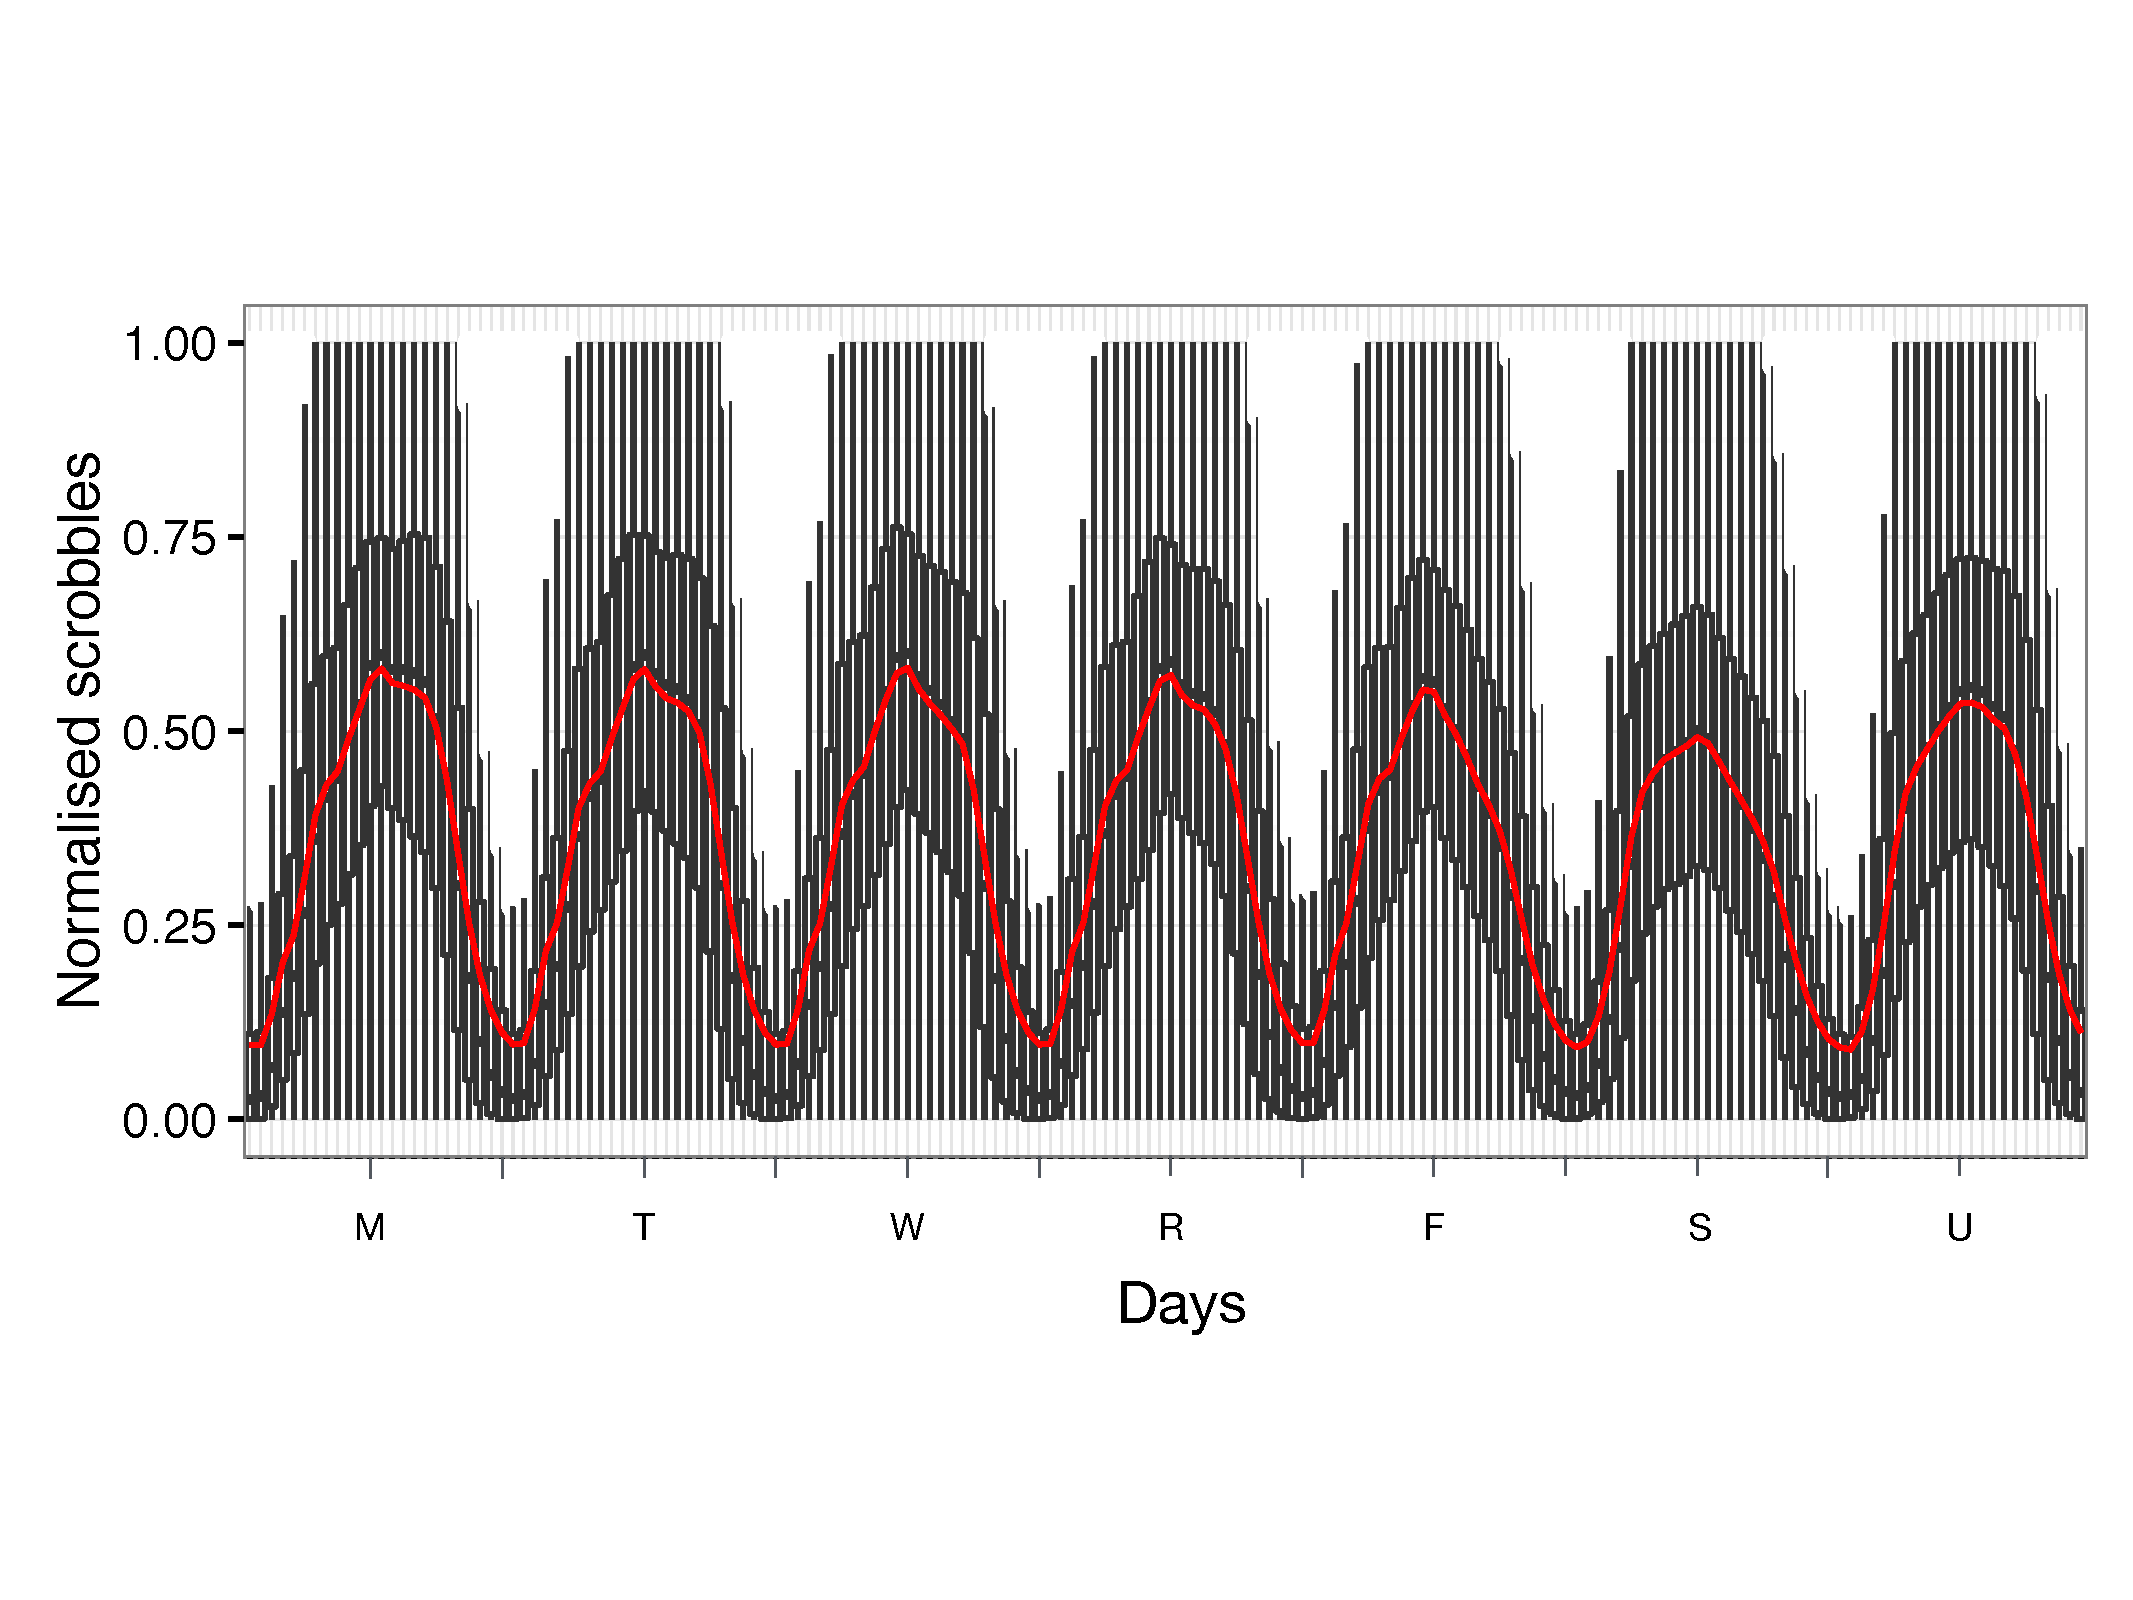
\includegraphics[width = 0.775\textwidth]{weekly_aggregated_UK_axis.jpg}
	\caption[Normalised per-week hourly aggregated number of scrobbles for UK listeners]{Normalised per-week hourly aggregated number of scrobbles for UK listeners (N = 42K). The red curve shows the normalised average number of scrobbles per hour over a week. The boxplots show median and quartiles per hour. We used this time series as the control time series for the TZ0xCORR time zone normalisation approach.}
	\label{fig:weekly_aggregated_UK_axis}
\end{figure}



These findings are contrary to what was previously reported by \textcite{north04uses}: people's exposure to music is greatest in the evening, particularly between 10 p.m. and 11 p.m., and on weekends. Furthermore, \textcite{sloboda01functions} found that people were not exposed to music at all while they were working, but mostly when they were at home. However, both studies were of a much smaller scale in terms of number of participants and the length of the period of music listening histories covered. 
Furthermore, those studies were developed more than a decade ago and music consumption behaviour has since changed to a very great extent. 
Music is nowadays consumed ubiquitously by means of portable devices accessing music streams through the Internet, and listeners seem to be willing to pay, or be exposed to ads, for accessing these services \autocite{wikstrom13music}. This behavioural change implies that people now can listen to music in any place with an Internet connection.

% there is no overlap between the CI error bars for peak and valleys in day and night, and so we found statistically significance support to our second assumption that stated that listeners generated less music logs songs during the night time than during the day.

We decided that the behavioural changes observed in the weekly aggregation preserved more information than the daily aggregation series. As a result, we decided to use the weekly time series as the control time series to estimate world users time zones using the TZ0xCORR approach.
Hence, we computed the lag in the number of hours needed to obtain the highest correlation between each user's aggregated music listening history and the TZ0 users control time series. 





% \begin{figure}[ht!]
% \vspace{1em}
% \centering
% \includegraphics[width = 0.75\textwidth]{5_clusters_20K.png}
% \caption{Clusters of listener's daily listening profile.}
% \label{fig:cluster_listeners}
% \end{figure}



% USING THE DAILY APPROACH INSTEAD OF THE WEEKLY ONE GAVE A LARGER PEAK AT TZ0, check http://thr.vigliensoni.com/?paged=6

% Also, check all the development blogged in http://thr.vigliensoni.com/?paged=6

In Figure \ref{fig:listenerstimezonebytz0weeklycorrelation} we show the estimated distribution of the overall listeners' time zones.	
\begin{figure}[!h]
% \vspace{1em}
\centering
\includegraphics[width = 0.9\textwidth]{listeners_tz_xcorr.pdf}
\caption[Distribution of the time zones for all users of the dataset]{Distribution of the time zones for all users of the dataset (N = 594K), estimated with cross correlation between their hourly weekly aggregated music listening histories and the average music listening histories from users in time zone 0.}
\label{fig:listenerstimezonebytz0weeklycorrelation}
\end{figure}
We can see a peak in the estimated time zone from where people was scrobbling at time zone GMT +0, with about 17 percent of the dataset users. Although just a few countries belong to that time zone, there are many countries in the Central European time zone that may have been merged because of their time shift in the Summer time due to the observance of the daylight saving time,  which represents roughly half of the year.
Another possibility for the large peak has to do with the actual correlation process: listening histories from people in close time zones got correlated without any lag due to individual shifts in their everyday life schedule.
The figure also shows that the TZ0xCORR approach estimated that many users were at $\pm$1 GMT and that there were many people spread between [-6, -3] GMT and [+6, +11] GMT. 

All in all, a large proportion of the listeners were estimated to be within time zones corresponding to Western Europe, but also spread out throughout the different time zones in America. The dataset did not seem to have many listeners from Asia. Finally, the shape of the people's estimated time zone seems to follow the distribution of users per country we showed on Figure \ref{fig:6_listeners_per_country}, where the majority of listeners in the dataset did self-report to be in the US and Western Europe.





% \begin{figure}[htb]
% 	\hspace{-1.5em}
% 	\epsfig{file=plots/listeners_extracted_timezone.png, width=3.5in}
% 	\caption{Time zone distribution for 594K listeners when cross correlating their aggregated weekly listening history with the average profile from listeners in time zone 0.}
% 	\label{fig:listenerstimezonebytz0weeklycorrelation}
% \end{figure}






\subsubsection{Local minima approach}
Based on the assumption that there is a smaller likelihood of people scrobbling at night compared to during the day, we developed a different method to estimate the time zone of users of the dataset. 
In this approach, we searched for the local minima indexes in the weekly aggregated listening profiles.
% , with a moving neighbourhood time period of 12 hours. %GVM:???
These minimum values provided a metric about when people actually submitted fewer music logs, probably because they were sleeping. 
Since we also expected that listeners changed their behaviour slightly on weekends---being different than on weekdays---we focused our analysis in extracting the local minima in weekdays only.

We implemented this approach by using the ``Wavelet Methods for Time Series Analysis'' (WMTSA) R package.\footnote{Wavelet Methods for Time Series Analysis (WMTSA) R package available at \url{http://CRAN.R-project.org/package=wmtsa}} Starting from a time series, the {\tt wavCWTPeaks} peak detection method of the package returns a matrix with the local maxima or minima indexes and their values. We retrieved the minima indexes from the weekly aggregated listening profiles, and normalised these indexes to the range [-12, 11] in order to have them within the range of a day. 
Then, we averaged and rounded these normalised minima indexes to an integer value. This final number was assumed to correspond to the estimated time zone for each listener. 
Averaging and rounding the multi local minima points allowed us to overcome the following problems: (i) minima that were not retrieved, because the effectively retrieved points were used for the final estimation; and (ii) false positive minima, because these values were averaged with the true positives, and so their effect was minimised. 


After implementing this approach, we realised that the local minima indexes of listening profiles with ``flat zones'' (i.e., valleys in a listening profile with no substantial change for a period of time) were usually at the beginning rather than at the middle or the end of the ``flat zones.'' 
In order to address this issue, we implemented a variant of the local minima approach that computed the local minima for the original time series of the weekdays, as well as its reversed version. The indexes obtained with this backward version were reversed again, and averaged with those retrieved by the forward version.
We expected that this method would be able to estimate the index at the middle for each one of the ``flat zones.'' 
The variant that calculated the time zone based on only the forward time series was named forward local minima (FF\_LM). The approach that calculated the time zone based on the forward and backward time series was named forward-backward local minima (FB\_LM).

\begin{figure}[!h]
% \vspace{1em}
\centering
\includegraphics[width = 0.85\textwidth]{local_minima_C.pdf}
\caption[Time-zone normalisation, local minima approach and variants]{Local minima approach and variants. Red dots indicate the daily minima indexes during weekdays, blue dots indicate the daily minima of the reversed time series, and green dots the average of the forward and backward time series minima indexes. The FF\_LM time zone estimation variant was based on the integer average of red minima indexes within a day. The FB\_LM variant was based on the integer average of green minima indexes.}
\label{fig:local_minima}
\end{figure}


In Figure \ref{fig:local_minima} we show a weekly aggregated listening profile. Red dots show the found minima during weekdays, blue dots show the minima indexes using the reversed version of the time series, and green dots show the average of the forward and backward versions. The FF\_LM time zone estimation is based on the integer average of red minima indexes within a day. FB\_LM is based on the integer average of green minima indexes.



\subsection{Seasonal decomposition}
In addition to the previous experimental factors for testing the best approach to identify time zones, we also employed time series decomposition to isolate the cyclic seasonal data from any trend and noise in the weekly aggregated music listening profiles. 
In other words, we also evaluated if removing the noise and trends of the profiles would improve the performance of any of the previously detailed approaches for time zone normalisation.
As a result, we ended up with raw and seasonal variants for each of the approaches, either based on the time-zone-0 (TZ0) cross correlation, or local minima (LM). All in all, we evaluated these two different main approaches and their variants.
% : TZ0xCORR, FF\_LM, FB\_LM, SEAS\_TZ0xCORR, SEAS\_FF\_LM, SEAS\_FB\_LM. 
In Table \ref{table:TZ-method-summary-cropped} we show a summary of the different approaches and variants, as well as an brief description of each method.

\begin{table}[!h]
% \vspace{1em}
\centering
\caption{Summary of methods for time-zone normalisation.}\label{table:TZ-method-summary-cropped}
\includegraphics[width = 1.00\textwidth]{TZ-method-summary-cropped.pdf}
\end{table}

\subsection{Experimental comparison}
We designed an experiment with the purpose of comparing the performance of all the approaches and their variants in identifying the time zones where weekly aggregated music listening patterns were generated.
To accomplish our goal, we designed an experiment in which we created a ground truth of time zones by randomly selecting a subset of listening histories from the dataset, aggregating their data into a week, and manually labelling each one of these profiles in a time zone within the range [-12, 11]. We followed \textcite{cochran77sampling} and estimated that a sample size of 384 listening histories would give us 95 percent confidence interval at $\pm$5 percent error.

To annotate the time zone for each listening profile, we visually inspected the time series and carefully paid attention to the assumptions already described: (i) listeners, in general, submit fewer music logs at night; (ii) people, in general, share a common pattern of music listening. We also assumed that people's behavioural patterns of listening change on weekends and so we only paid attention to weekday cycles. We named this subset the control dataset. 

Although we expected that labelling listeners' time zones would be straightforward, we realised that their annotation was difficult. Most people in the control dataset had cyclic patters but some had slight changes in their weekly profiles. As a result, choosing one specific time zone was not obvious. Furthermore, a few listeners did not have a clear cyclic pattern at all. 
In order to exemplify some this variability, in Figure \ref{fig:tz_eight_users} we show the weekly aggregated listening profile of six listeners supposedly to be in different time zones. While it seems easy to estimate the time zone of listeners in the upper row, the annotation is problematic for the ones in the bottom row. 

\begin{figure}[!h]
\vspace{1em}
\centering
\includegraphics[width = 0.75\textwidth]{8_aggregated_weekly_behaviour.pdf}
\caption[Example of weekly aggregated music listening profiles of six listeners]{Weekly aggregated music listening profiles of six listeners in our control dataset. While the time zones for the profiles in the upper row was easily estimated by visual inspection, the estimation for the lower row profiles was problematic.}
\label{fig:tz_eight_users}
\end{figure}

After we created the control dataset, we proceeded to compute the time zones with the six aforementioned approaches. In order to evaluate the different approaches, and given the limited ``ground truth'' data, we used a bootstrapping technique. This technique makes use of re-sampling for computing an estimator such as the confidence interval or standard error when analysing small datasets with sparse prior information or unclear distributions \autocite{henderson05bootstrap}.
As a result, we took random samples with replacement from the original population of listening profiles, creating 1,000 random populations of 384 listening profiles each. 

We wanted to calculate the performance of each method not only by measuring the percentage of perfect matches between the estimated time zones and to the ones in the control dataset, but also by how close those were to each other. In other words, an error in the estimation of $\pm$1 hour should be less important than a larger difference. Hence, we quantified the performance of each approach by computing their time difference in hours. For example, if both the computed and the manually labelled weekly listening profile had the same time zone, their time difference was zero, but if the computed profile was shifted by two hours to the left, their time difference was -2 hours.



In Figure \ref{fig:1000pop_6met_mn_sd_24timediff} we show the performance of the six approaches in identifying time zones of listening profiles. 
Bars and colours indicate the time differences in hours, ranging from [-12, 11], where a zero-hour difference is orange. 95 percent CI error bars show upper and lower limits for 1,000 bootstrap samples replicated from the original sample of 384 listening histories using bootstrap at $\alpha$ = 0.05. 


\begin{figure}[!h]
% \vspace{1em}
\centering
% \epsfig{file=plots/1000_pops_6_methods_per_24_timediff_PRINT.pdf, width=\textwidth}
\includegraphics[width=1.0\textwidth]{1000_pops_6_methods_per_24_timediff_PRINT.pdf}				
\caption[Performance of six approaches for time-zone normalisation]{Performance of six approaches in identifying time zones of listening profiles. The plot shows percentage and 95\% CI error bars for each possible time difference between the manually labelled control dataset and the computed time zones for 1,000 bootstrap samples taken from 384 listening histories.}
\label{fig:1000pop_6met_mn_sd_24timediff}
\end{figure}






It can be seen in the figure that the largest percentage of correctly computed time zones (i.e., time difference was zero) was achieved by TZ0xCORR and SEAS\_TZ0xCORR, showing significant differences with the other approaches. 
However, when analysing the performance of all methods with a tolerance of $\pm$1 hour, the FB\_LM and FF\_LM approaches---methods based on the assumption that people scrobble less frequently at night---had a much better performance. In fact, these methods appropriately computed the time zones, with a one-hour window tolerance, for 75 and 70 percent of the dataset respectively. 

There was no significant difference between models for aligning local minima. Hence, the forward-backward approach we implemented to overcome the estimation of minima of listeners with ``flat zones'' was not effective. 
%In fact, if we look in Fig. \ref{fig:1000pop_6met_mn_sd_24timediff} to all four \emph{local minima}-based methods (i.e., \emph{FF\_LM}, \emph{FB\_LM}, \emph{SEAS\_FF\_LM}, and \emph{SEAS\_FB\_LM}) we can see that they peak at a time difference of $-1$. 
%Pragmatically, if we just delay the time zones by $+1$ and use any of these four methods, we will obtain an improvement of 10 percent in the time zone recognition. 
The seasonally decomposed versions of the local minima approaches had a poorer performance than their raw counterpart, implying that there was information in the full data that was lost when we decomposed the time series. This data may be helpful for determining the time series of the weekly time series and so it should not be discarded.
Overall, the best approach was based on finding the local minima of weekly aggregated listening profiles, which was based on the assumption that people share hours of sleep at night. This approach recognised correctly 75 percent of the time zones with $\pm$1 hour of tolerance. 

Some drawbacks may be raised concerning our experimental design and analysis. 
First, the time zone of listeners can be not fixed, especially when considering long listening histories. People may travel for vacations or work while still being submitting music logs, or they may move to a different time zone indefinitely. Although the aggregation of long listening histories minimises the former issue, it can not cope with the latter. Also, this approach may also be biased against workers who work a night shift. It would be interesting to investigate the actual percentage of people migrating to different time zones and working a night shift, and see if this point could have an effect in our analysis. 


Second, in spite of the fact that individual schedule variation (e.g., morning people as opposed to night people) could possibly exceed small differences in time zones, the approaches we designed for identifying time zones in people's listening profiles can still be used to know the shift of these cyclic listening patterns in time, allowing straightforward comparison between them. 
As a consequence, having the listening histories aligned in time permits to easy comparison of listening patterns because the shift between them will be minimised. This may be helpful, for example, to profile listeners by the proportion of listening logs they submit during a day or a week. This may provide a degree of information about people's listening habits, data that could be used as a signal that may be used by music recommendation services to tailor their recommendations to the specific situation of the listener.


In this chapter we described the creation of the MLHD, a very large dataset of full music listening histories. We presented the criteria for the data collection, acquisition, cleaning, and the integration of the data. We then provided insights about the demographic characteristics of users in the dataset, and we investigated about different approaches for performing a temporal alignment of the music listening histories that will allow us to compare them directly.

In the next chapter we will formalise a set of features to describe some of the aspects of the music listening behaviour of listeners in the MLHD, and we will show different patterns of these features that can be found at the country, age, and gender level. 
We will finalise the next chapter by evaluating whether the demographic, profiling, as well as contextual features extracted from the music listening histories can improve the accuracy of a series of music artist recommendation models.

% \subsection{Temporal distribution of music logs}
% Analysing the temporal distribution of music logs shows that listeners in our dataset are less active during night, as expected, but there was no significant difference between days of the week. This distribution of music logs per hour of the day and the of the week is similar to other music listening behaviour datasets, such as the MMTD \textcite{hauger13million}.
% TODO: write about the weekly aggregated temporal distribution. 

% TODO: write about the clustering of daily and weekly aggregated music listening histories. how they cluster and why i did not use them for profiling users in the dataset. Ex: http://thr.vigliensoni.com/?paged=5



% \section{Conclusions}\label{sec:5-conclusions}
% TODO!!!!























% %========== Listener aware music recommendation
\typeout{}
% \setcounter{page}{1}
\setcounter{chapter}{4} % for having chapter as number 4 even with no previous chapters
% \newpage\null\thispagestyle{empty}\newpage
%!TEX root = ThesisEx.tex
% \resetdatestamp
\chapter{Listener-aware recommendation}\label{ch:6-listener-aware-music-recommendation}
% \section{Recommender systems}\label{section:ch5}
% \vspace{0.05cm}
\graphicspath{{./figs/ch8/}}
% Converting implicit preference to explicit 1 to 5 level liking scale
% Should I explain here how I'm using user-side features or in the  chapter of context-aware recommendation?
% More information on user profiling: EchoNest Taste profile (in alpha release) https://web.archive.org/web/20160312191903/http://developer.echonest.com/docs/v4/catalog.html
% Diversity - measures the overall diversity of a fan’s listening by mapping the overall distance across the musical styles of the listener. Mainstreamness - measures the overall familiarity of a user’s listening activity to determine preference for either mainstream or more obscure music. Freshness - measures listening habits to determine how much a user cares about new album releases vs. sticking with older music. Adventurouness - measures how open the listener is to music outside of his or her musical comfort zone.
% Also check the white paper ~\autocite{echonest13how}, and how EN is profiling ``high value'' listeners' interests such as: social causes, concerts, beer, wine, and liquor, green/eco, outdoor, fashion, sports, fitness, travel, parenting, and personal finance.
% \subsection{Recommending music according to profiles of listeners}
The modelling of users for multimedia information retrieval systems has been a research topic since the first International Symposium on Music Information Retrieval (ISMIR) in 2000. 
In that meeting, \textcite{chai00using} observed that to create modern, more efficient, and personalised music information retrieval systems, the modelling of users would be necessary because many features of multimedia content delivery are perceptual and user-dependent. 
As a result, they proposed a language capable of expressing different types of user information that also allowed the interoperability between music information retrieval systems to share these user profiles.


Sixteen years after the first ISMIR meeting, the landscape of music consumption has changed enormously and the idea of sharing user models and profiles now seems quite na\"{\i}ve.  The rise and fall of peer-to-peer networking led to the reinvention of the music industry: the paradigmatic music pro\-duct was no longer a full album in a physical format, but individual music files available in online digital music stores. 
Thanks to the miniaturisation of portable media players and also to almost ubiquitous Internet access, a change of paradigm in music consumption has happened again, and people seem to not want to pay for individual tracks. Instead, they are willing to pay for services that allow them to access, search, and discover music items---artists, albums, or tracks---within large repositories \autocite{wikstrom13music}. 

On-demand digital music streaming services are currently the fastest growing sector of the global music industry \autocite{ifpi15global} and in 2015, the digi\-tal revenues that these systems generate overtook the income from physical music goods for the first time in music industry history \autocite{ifpi16global}. 
The on-demand music streaming landscape these days seems to be a lucrative battlefield, and one on which many companies want to compete.
% For Ek, the streaming model is more like modern advertising 
% Spotify's streaming patent \autocite{ehn12peer}
However, most of the profits from the streaming model of business do not rely on the number of subscribers to these systems, providing the best experience to access music, or on finding the best next song that a listener would like to hear. 
Since the majority of the listeners' accounts in music streaming services use the ``free'' or ``freemium'' business model---advertisement-supported basic streaming services---a large share of the income of music and media streaming companies comes from targeting ads more precisely at listeners \autocite{rutter16music}.
All in all, people are no longer passive observers but direct participants in the battlefield that is the digital media and music streaming landscape.
% \todo{DB: I'm not sure what you mean here}
In fact, the traded goods in this business are individual profiles and psycographic traits (i.e, interests, lifestyle, personality, values) which are extracted from correlating their listening habits with their sociographic characteristics \autocite{prey16musica}. 
As a result, listeners are the source of information, but they also are the final target for all the commercials these companies are making money from. 


The main research question of this dissertation is about the degree of impact of using demographic, profiling, and contextual features from listeners in improving the performance of automated music recommendation systems.
However, these features may also be used to profile and model a user's traits for potentially musically-unrelated purposes, such as the aforementioned ad customisation.
Since the customised promotion of products and services is driving the music industry business, while not directly discussed, the research presented in this dissertation may have applications beyond automatic music recommendation.

In Section \ref{sec:6-listener-demographic-profiling-and-contextual-features} we will describe a set of listening behavioural features that we developed to characterise and profile listeners. We will formalise them and show how they can be used to find patterns at the country and age-group levels. In conjunction with self-declared demographic features and basic forms of listening context extracted from  aggregated listening patterns, in Section \ref{sec:6-experiment-implementation} we will evaluate if the use of these signals improve the accuracy of a recommendation model.



\section{\textit{User-centric} features}\label{sec:6-listener-demographic-profiling-and-contextual-features}
Traditional automated music recommendation systems embedded in most music streaming services still typically rely on the accuracy of statistical models learned only from the past preferences of users on music items. 
However, \textcite{lee15user, fuller16elucidating} found that  there are different types of listeners in terms of how they consume music, and so it seems reasonable to think that each type of listener needs a different type of recommendation.
Therefore, additional sources of data such as the demographic attributes of listeners, and their listening behaviour and context, may encode information about people and their listening habits and preferences that can be used to improve the performance of a music recommendation model. 




Now we will discuss the impact of using demographic and profiling characteristics---\\which in the context of this dissertation have been referred to as \emph{user-side} or \emph{user-centric} features---in improving the accuracy of a music recommendation model.
User-centric features were extracted from listeners' self-declared demographic data and a set of custom-built profiling features characterizing their music listening behaviour. 
Models based on latent factors and all combinations of user-side features were learnt by using data from the Music Listening Histories Dataset (MLHD) described in Chapter 4.
% ~\ref{ch:5-music-listening-histories-dataset}
Finally, music listening histories were aggregated into different time spans to evaluate if the accuracy of the models changed in different periods of listening. 





\subsection{Music listening behavioural features design}\label{sub:ch6-profiling-features-design}
We hypothesised that by better understanding the listening behaviour of people, we will be able to more accurately model a user's needs. Hence, the recommendation of music items can be tailored to each listener, and the prediction accuracy will likely improve. 
    
A set of five computational features tailored to characterise listening behaviours were described in \textcite{echonest13how}, and presented as part of The Echo Nest Taste Profile API project.\footnote{Deprecated after Spotify acquired The Echo Nest, but available through Internet Archive's Wayback Machine at \url{https://web.archive.org/web/20150707212616/http://developer.echonest.com/docs/v4/tasteprofile.html}} These features were developed to identify the listening characteristics that best described a listener, allowing music streaming services to recognise ``high-value'' users (i.e., the highly engaged listeners of a music service) and groups of users with similar patterns of music listening behaviour. According to The Echo Nest, the ultimate goal of these profiling features was to identify ``psychographic characteristics'' of the high-value users to monetise this group of listeners via ``targeted advertising.''
% Is not better if I don't present them for more novelty?
The set of features that The Echo Nest designed to describe listeners were \textit{adventurousness} (i.e., how open the listener is to music outside their ``musical comfort zone''), \textit{diversity} (i.e., how varied the listener’s preferred styles and genres are), \textit{freshness} (i.e., the listener's preference for new and recent artists versus older music), \textit{locality} (i.e., describes the spread, worldwide, of where the listener's preferred artists come from), and \textit{mainstreamness} (i.e, the listener's affinity for well-known artists versus obscure artists). 
Although The Echo Nest provided detailed documentation about how they calculated their custom-designed acoustic features based on the work by \textcite{jehan05creating}, they did not provide any implementation details about how they calculated their listening profile features. 
The Echo Nest's Million Song Dataset Taste Profile subset supplied listening information for a large amount of listeners, but only in the form of playcounts without any temporal information. 
Finally, The Echo Nest API\footnote{The Echo Nest API is not available any more. However, the API documentation can still be accessed at \url{https://web.archive.org/web/20160407081912/http://developer.echonest.com/docs/v4/index.html#overview}} was taken down shortly after Spotify acquired The Echo Nest, and so there is no way of correlating a song's feature values with a listener's behavioural features using their API. The obscurantism about how they calculated these listening behavioural characteristics may be an indication of the high value of this information.

In order to evaluate if music listening behavioural characteristics can be used to improve the performance of a music  recommendation model beyond plain collaborative filtering (CF), \textcite{schedl15tailoring} proposed another set of custom-designed features that attempted to describe aspects of music listening behaviours in relation to music artists.
Although the authors computed continuous values for their listening-centric user features, they grouped the listeners into categorical levels according to their feature values, perhaps losing some information in this process. Then, they compared the performance of single and combined recommendation algorithms by varying the number of recommended artists between one and 1,000.
As a result, they evaluated different recommendation approaches only in regard to the set of more popular artists with listeners grouped in fixed listening categories. 
Some of the features proposed by the authors considered only the number of playcounts, but did not consider the ranking of the music items within the overall ranking or within each listener's ranking. Therefore, biases in the distribution of items could be amplified during the feature computation.
The authors planned to integrate their listening behaviour features as user-centric features directly into recommendation algorithms based on matrix factorisation, however there are no publications with this implementation so far.

Now we will describe our efforts attempting to represent some characteristics of music listening behaviours. Attending to the conceptual design and implementation details of listening behavioural features on previous studies, we used continuous feature values to express the precise value of a certain listening behaviour characteristic in relation to a music item, and we considered the position of the music items within each listener's  ranking as well as the overall ranking . Finally, we integrated these feature values directly into a recommendation model based on matrix factorisation (see Subsection \ref{sub:matrix}) in order to predict the preference values on all available items.

We restricted ourselves to designing four novel features to describe listener behaviours: \textit{exploratoryness}, \textit{mainstreamness}, \textit{genderedness}, and \textit{fringeness}. 
Values for these features were computed for the three types of  music items in the dataset: tracks, albums, and artists. Therefore, each listener's listening was described by a vector of 12 values.
In the following sections we will describe the goals behind each of these features, give details about their implementation, visualise data patterns, and provide some analysis of the results. 

\subsubsection{Exploratoryness}\label{subsec:exploratoryness}
	To represent how much a listener explores different music instead of listening to the same music repeatedly we developed the \emph{exploratoryness} feature. 

	For each user $x$'s listening history, let 
    $L$ be the number of submitted music logs,
    $S_k$ be all submitted music items of type $k$, where $k$=\{tracks, albums, artists\},
	$s_{k,i}$ be the number of music logs for the given music item key $k$ at ranking $i$. 
    The ranking was the ordered set of music items,  from the most highly listened to the less frequently listened item. This information was computed directly from the music items frequencies within each listening history for each listener.
    We computed the exploratoryness $e_{x,k}$ for listener $x$ on a given music item of type $k$ as:
    	\vspace{1em}
		\begin{equation}
			\abovedisplayskip=2pt plus 3pt minus 9pt
			\label{eq:exploratoryness}
			e_{x,k} = 1 - \frac{1}{L}\sum_{i=1}^{S_k}{\frac{s_{k,i}}{i}}
		\end{equation}
    




Exploratoryness  returns a normalised value, with values closer to zero for  users listening to the same music item again and again, and values closer to one for users with more exploratory listening behaviour. 
% ~\citeauthor{baur12listening} found that one of the listening factors that influences music preference is what they called variety, how often songs, albums, and artists are repeated. Since their approach was based on principal component analysis, there was no mathematical formulation for this features and also there was no explanation about how they arrived to this concept.




% \begin{figure*}[t]
% % \hspace{-1.5em}
% \epsfig{file=2_3_features_age_groups.pdf, width=\textwidth, keepaspectratio}
% % \caption{Feature extraction for listeners in the dataset. (a) Artist exploratoryness of listeners by age, (b) track mainstreamness of listeners by age, (c) artist genderedness of listeners by age and gender. In all cases error bars show $\pm$1 SD and 95\% ci.}
% \caption{Feature means and 95\% CI bars for a random group of listeners in our dataset. Each age group has 1000 listeners and error bars were calculated by taking 1000 populations replicated from the original sample using bootstrap. (a) Artist exploratoryness by age group of listeners, (b) artist mainstreamness by age groups of listeners, and (c) artist genderedness by age group and gender of listeners.}

% \label{fig:3_features}
% \end{figure*}	


% Fig. \ref{fig:3_features}

	% \begin{figure*}[t]
	% 	% \hspace{-1.5em}
	% 	\epsfig{file=plots/3_features.png, width=\textwidth, keepaspectratio}
	% 	\caption{Feature extraction for listeners in the dataset. (a) Artist exploratoryness of listeners by age, (b) track mainstreamness of listeners by age, (c) artist genderedness of listeners by age and gender.}
	% 	\label{fig:3_features}
	% \end{figure*}	





\subsubsection{Mainstreamness}\label{subsec:mainstreamness}
	With the goal of expressing how similar a listener's listening history is to what everyone else listened to, we developed the \emph{mainstreamness} feature. It analyses a listener's ranking of music items, and compares it with the overall ranking of artists, albums, or tracks, looking for the position of co-occurrences. %Music logs in the database without IDs are not considered.
	

	For each user $x$'s listening history, let 
	$N$ be the number of logs of the music item ranked first in the overall ranking,
    $L$ be the number of submitted music logs,
%     $S$ be all music items keys for any of the three types, 
	$S_k$ be all submitted music items of type $k$, where $k$=\{tracks, albums, artists\},
%     $s_i$ be the number of music logs of music item ranked at position $i$ , and 
	$s_{k,i}$ be the number of music logs for the given music item key $k$ at ranking $i$, and
%     $o_i$ be the number of music logs in the overall ranking of music items ranked at position $i$. 
	$o_{k,i}$ be the number of music logs in the overall ranking of music item type $k$ ranked at position $i$.
    	We defined the mainstreamness feature $m_{x,k}$ for listener $x$ on a given music item of type $k$ as:
		\begin{equation}
% 			\abovedisplayskip=2pt plus 3pt minus 9pt
			\label{eq:mainstreamness}
			m_{x,k}=\frac{1}{N L}\sum_{i=1}^{S_k}{s_{k,i}}{o_{k,i}}
		\end{equation}



Listening histories of people with a music item's ranking similar to the overall ranking receive mainstreamness values closer to one. Listeners' mainstreamness whose ranking differs more from the overall ranking receive values closer to zero.
As mainstreamness depends upon the overall ranking of music items we computed the overall ranking from all music logs in MLHD for the three music entities in the dataset. In Table \ref{table:artist_ranking} we show the first 20 artists and their total number of logs in the ranking of artists. 

\graphicspath{{./figs/ch6/}}
\begin{table}[!h]
% \vspace{1em}
\centering
\caption[20 top-ranked artists in the MLHD dataset]{20 top-ranked artists in the MLHD dataset. The ``Total logs'' column refers to the total number of logs, in millions, for the particular artist in the dataset.}\label{table:artist_ranking}
\includegraphics[width = 0.60\textwidth]{ranking_artist_cropped.pdf}

\end{table}

% \newpage
As expected, the first places of the ranking were populated with highly known music artists. However, although there were a number of artists that are considered ``classic'' (e.g., The Beatles or Pink Floyd), several classic music artists were missing in the top 20 positions of the ranking (e.g., Rolling Stones or Michael Jackson). 
% It is also unlikely that users in the MLHD dataset have listened to music artists such as The National more than to Madonna, for example.
Moreover, it is peculiar that all the highly listened artists in the dataset are usually referred to as Pop or Rock artists. There is no representation of other popular genres among young people, such as Electronic or Hip-hop. 
These characteristics of the dataset may indicate that there is a bias in the listeners that are represented in the MLHD dataset. Since the population sample of the dataset is big, we suspect that there is a bias of towards Pop and Rock artists in the Last.fm users. However, we believe that every music streaming service has a specific bias. The Soundcloud music service, for example, is known for being a niche place for Electronic and Hip-hop artists and listeners.





In Table \ref{table:album_ranking} we show the ranking for the 20 most popular albums in the MLHD dataset. 
If the ranking of artists was clearly dominated by very popular artists, the ranking of albums showed a different arrangement. A number of apparently not-so-popular albums occupied the first places of the ranking. 
This characteristic of the ranking of albums in the dataset indicates that the ranking of artists is obviously ranked by the aggregated number of submitted logs for all the releases by an artist. Therefore, music artists with a long and consistent trajectory of good releases reach the first places of the ranking. 
On the other hand, artists with a shorter trajectory or with a few popular releases do not reach the ranking of artists but some of their releases are heavily listened. As a results, they get into the first places of the ranking of albums (e.g., Bon Iver or Paramore).

\graphicspath{{./figs/ch6/}}
\begin{table}[!h]
% \vspace{1em}
\centering
\caption[20 top-ranked albums in the MLHD dataset]{20 top-ranked albums in the MLHD dataset. The ``Total logs'' column refers to the total number of logs, in millions, for the particular albums in the dataset.}\label{table:album_ranking}
\includegraphics[width = 0.9\textwidth]{ranking_album_cropped.pdf}
\end{table}



It is also interesting to notice that the album ``xx'' by the artist ``The xx'' appears twice in the top 20 ranking. By reviewing this issue closely, we found out that this release appeared at least twice in our dataset, with two different MusicBrainz identifiers (MBIDs) that were not linked to each other.
We reported this issue to Last.fm and MusicBrainz. We did not receive a response from Last.fm, but MusicBrainz replied that some items in their database have  different MBIDs because of processes of merging and splitting. 
For example, if by any reason a user merges the entity Bob Marley with the entity Bob Marley and the Wailers---and this merge is accepted by the MusicBrainz community---the new entity Bob Marley will be reachable by three different MBIDs: the one from the original Bob Marley, the one from Bob Marley and the Wailers, and also from the newly created from the merging process.\footnote{In fact this happened once but the merge was reverted since it was clearly a mistake (\url{https://chatlogs.metabrainz.org/brainzbot/metabrainz/2015-12-04/?msg=3422608&page=1})} 
This behaviour occurs because MusicBrainz do not delete the previous entities, nor their MBIDs, from their database.
MusicBrainz manages to return the latest MBID when someone queries the API with an entity's former MBID by means of redirection tables\footnote{Documentation about the MusicBrainz schema and how redirect tables work is available at \url{https://wiki.musicbrainz.org/MusicBrainz_Database/Schema#Schema}} (e.g., MusicBrainz redirects the MBID used by Last.fm for Britney Spears (\texttt{2f4f5d16-7102-4110-97fd-f5c365d6bb26}) to the latest one on the MusicBrainz database (\texttt{45a663b5-b1cb-4a91-bff6-2bef7bbfdd76})).\linebreak Redirections are not directly available from the MusicBrainz API, but they can be accessed by downloading and using a local copy of the MusicBrainz data\-base.\footnote{Documentation about how to download and set up a local instance of the MusicBrainz database is available at \url{https://musicbrainz.org/doc/MusicBrainz_Database/Download}}
Last.fm, on other hand, does not work with redirections and so they seem to store versions of the same music entity using different MBIDs, and also does not store newly created MBIDs for merged entities.
All in all, if the number of logs of the release ``xx'' by the band ``The xx'' is aggregated, it becomes the most listened album in the dataset. 
% However, for calculating the rankings we did not perform this matching.


 In Table \ref{table:track_ranking} we show the ranking for the 20 most popular tracks in the MLHD dataset. The ranking exhibits a similar behaviour to the ranking of albums, with only a small number of ``classic'' tracks in the first places of the ranking.

\graphicspath{{./figs/ch6/}}
\begin{table}[!h]

\centering
\caption[20 top-ranked tracks in the MLHD dataset]{20 top-ranked tracks in the MLHD dataset. The ``Total logs'' column refers to the total number of logs, in millions, for the particular tracks in the dataset.}\label{table:track_ranking}
\includegraphics[width = 0.9\textwidth]{ranking_track_cropped.pdf}
\vspace{1em}
\end{table}




\subsubsection{Genderedness}\label{subsec:genderedness}
	With the aim of expressing how close a listener's listening history is to what females or males are listening to, we developed the \emph{genderedness} feature. 
    The genderedness feature computation basically relies on mainstreamness, but instead of computing just one overall ranking from all listeners, it uses two rankings: one made with music logs from listeners self-declared as female, and another one made with music logs from listeners self-declared as male. 

	For each user $x$'s listening history and music item of type $k$, let
	$m_{x,k,male}$ be the mainstreamness computed with the male ranking,
	$m_{x,k,female}$ be the mainstreamness calculated with the female ranking.
   We defined the feature genderedness $g_{x,k}$ for listener $x$ on a given music item of type $k$ as:
          \vspace{1em}
			\begin{equation}
			\abovedisplayskip=2pt plus 3pt minus 9pt
			\label{eq:genderedness}
			g_{x,k}=m_{x,k,male} - m_{x,k,female}
		\end{equation}


\subsubsection{Fringeness}
We developed the \emph{fringeness} feature with the objective of expressing how much a user listened to rare music items. In other words, those items for which the Last.fm database did not have an MBID (see Figure \ref{fig:mbid_combinations_crop} for summary of the percentage of music logs with and without MBIDs for the different music items).

% Let $e_x$ be the number of scrobbles without IDs for music items, and $t_x$ the total number of music logs in the listening history for user $x$, the fringeness value $f_x$ can be expressed as: 
% 	\begin{equation}
% 		\abovedisplayskip=2pt plus 3pt minus 9pt
% 		f_x = \frac{e_x}{t_x}
% 	\end{equation}


	For each user $x$'s listening history, let 
%     $L$ be the number of submitted music logs,
    $S_k$ be all submitted music items of type $k$, where $k$=\{tracks, albums, artists\},
%     $s_i$ be the number of music logs for any given music item key at ranking $i$. 
	$F_k$ be the number of music logs of type $k$ without IDs in the Last.fm database.
    
    We defined the feature fringeness $f_{x,k}$ for listener $x$ on a given music item of type $k$ as:

	\begin{equation}
		\abovedisplayskip=2pt plus 3pt minus 9pt
		f_{x,k} = \frac{F_x}{S_x}
	\end{equation}


% \vspace{0.5cm}












\subsection{Profiling listeners}\label{sec:profiling}
\graphicspath{{./figs/ch6/}}
% Age seems now to be important.
% From \textcite{straw90popular}
% While the programming principles of Top 40 radio have long been regarded as appropriate to an audience dominated by adolescents, Top 40 programmers have, for the most part, conceived that audience in only the most general of demographic terms. Despite the rise of detailed demographic profiles of radio audience since the mid-1960s, Top 40 stations would continue, throughout the 1970s, to regard their adolescent listeners as the active core at the centre of a wider, general audience, rather than as a restricted demographic group with its own, specific appeal to advertisers. This general audience is often seen to be stratified, with, as its core, a group of adolescent listeners active in the monitoring of musical innovation and in the purchasing of musical recordings, but in their competition for advertising revenues Top 40 radio stations will usually identify themselves as having a "mass appeal."
To illustrate how the features we developed can be used to profile listeners, we calculated the exploratoryness, mainstreamness, genderedness, and fringeness for all users in the MLHD dataset,  for each one of the music entities. 
As we saw in Subsection \ref{sub:cleaning}, not all music logs within each listening history had a full set of MBIDs, and so we ended up using the total number of logs that had a MBID for the specific music entity at hand. 
In total, we used 93 percent of logs of the dataset when computing profiling features in relation to artists, 64 percent with albums, and 78 percent with tracks.


In Figure \ref{fig:mainstreamness_by_age} we show a boxplot summary of the calculated mainstreamness values by age, computed for all listeners in our dataset with self-declared age within [15, 54] years old.
We can see in the figure that younger people tend to have higher levels of mainstreamness, disregarding if the music item is an artist, album, or track. 
Since mainstreamness is based on comparing rankings of music items, this characteristic indicates that younger people tend to listen more to music items that are ranked higher in the overall ranking of music items. On the other hand, older people listen to music that is experienced less frequently, in general.
The mainstreamness feature value of all three music items diminishes steadily with age and tends to plateau when people get older.
The three plots in the figure also display an uneven change in the distributions of the computed mainstreamness for the population of listeners in their forties and fifties, as well as for 15-year-old listeners. 
The larger variability in these populations may be explained due to the much smaller number of music listening histories from listeners within those age ranges.

\graphicspath{{./figs/ch6/}}
\begin{figure}[!t]
	\centering
	\begin{subfigure}[b]{\textwidth}
		\centering
		\includegraphics[width=0.75\textwidth]{artist_mainstreamness.pdf}
        \caption{Artist mainstreamness by age}
        \label{fig:artist_mainstreamness}
	\end{subfigure}
    % \vspace{5pt}

	\begin{subfigure}[b]{\textwidth}
		\centering
		\includegraphics[width=0.75\textwidth]{album_mainstreamness.pdf}
        \caption{Album mainstreamness by age}
        \label{fig:album_mainstreamness}
	\end{subfigure}
    % \vspace{5pt}

	\begin{subfigure}[b]{\textwidth}
		\centering
		\includegraphics[width=0.75\textwidth]{track_mainstreamness.pdf}
        \caption{Track mainstreamness by age}
        \label{fig:track_mainstreamness}
	\end{subfigure}
    % \vspace{10pt}
	\caption[Summary of computed artist, album, and track mainstreamness]{Boxplots showing summary of the calculated artist, album, and track mainstreamness values by listeners' age, computed for all users in MLHD with a self-declared age within [15, 54] years old.}
	\label{fig:mainstreamness_by_age}
\end{figure}

% Boxplots are a summarised visual representation of batches of data. The central, horizontal line within each boxplot shows the median. The first and third quartiles (i.e., the 25th and 75th percentiles) are shown by lower and upper hinges. The extremes show about 99 percent of the total amount of the data distribution. Finally, the notches surrounding the median show a measure of the significance of the differences between the populations. If the notches do not overlap, the medians are significantly different at 95 percent confidence level \autocite{mcgill78variations}. 






We have to note that, since mainstreamness is defined based on the ranking of the music items in the whole dataset, the distribution of mainstreamness across age could be affected by the fact that the dataset is dominated by younger users. However, the mainstreamness feature tries to express the degree of similarity of a listener's history to what everyone else listened to, and so this behaviour is expected, particularly if the dataset population is biased towards a specific group.

\begin{figure}[!t]
	\centering
	\begin{subfigure}[b]{\textwidth}
		\centering
		\includegraphics[width=0.75\textwidth]{artist_exploratoryness.pdf}
        \caption{Artist exploratoryness by age}
        \label{fig:artist_exploratoryness}
	\end{subfigure}
    % \vspace{10pt}

	\begin{subfigure}[b]{\textwidth}
		\centering
		\includegraphics[width=0.75\textwidth]{album_exploratoryness.pdf}
        \caption{Album exploratoryness by age}
        \label{fig:album_exploratoryness}
	\end{subfigure}
    % \vspace{10pt}

	\begin{subfigure}[b]{\textwidth}
		\centering
		\includegraphics[width=0.75\textwidth]{track_exploratoryness.pdf}
        \caption{Track exploratoryness by age}
        \label{fig:track_exploratoryness}
	\end{subfigure}
    % \vspace{10pt}

\caption[Summary of computed artist, album, and track exploratoryness]{Boxplots summaries of the artist, album, and track exploratoryness by listeners' age, computed for all users in the MLHD with a self-declared age within [15, 54] years old.}
\label{fig:exploratoryness_by_age}
\end{figure}



The computed exploratoryness feature by age of listeners for artists, albums, and tracks is shown in Figure \ref{fig:exploratoryness_by_age}. The boxplots show that there is an increase in the exploratoryness of listeners for all music items while in their late teens and early twenties. This rise tends to plateau for young adults at about 30 years old. 
The variability in the medians increase for older people since the number of music listening histories is much smaller than for younger people, except for 15-year-old listeners.
Although the absolute values of exploratoryness are different for each music item, the shape of the increase in the population curves per age are similar, implying that the relation between exploratoryness and age is the same.
This characteristic seems to indicate that younger people tend to listen to the same music more repeatedly compared with older people. On the other hand, older listeners in the MLHD, listened to artists, albums, and tracks in a more diverse fashion, exploring more items. 


\graphicspath{{./figs/ch6/}}
\begin{figure}[!t]
	\centering
	\begin{subfigure}[b]{\textwidth}
		\centering
		\includegraphics[width=0.66\textwidth]{artist_exploratoryness_by_country.pdf}
        \caption{Artist exploratoryness by age and country of listeners}
        \label{fig:artist_exploratoryness_by_age_and_gender}
	\end{subfigure}
%     \vspace{10pt}

	\begin{subfigure}[b]{\textwidth}
		\centering
		\includegraphics[width=0.66\textwidth]{album_exploratoryness_by_country.pdf}
        \caption{Album exploratoryness by age and country of listeners}
        \label{fig:album_exploratoryness_by_age_and_gender}
	\end{subfigure}
%     \vspace{10pt}

	\begin{subfigure}[b]{\textwidth}
		\centering
		\includegraphics[width=0.66\textwidth]{track_exploratoryness_by_country.pdf}
        \caption{Track exploratoryness by age and country of listeners}
        \label{fig:track_exploratoryness_by_age_and_gender}
	\end{subfigure}
%     \vspace{10pt}

\caption[Artist, album, and track exploratoryness means versus age of listeners]{Exploratoryness mean for artist, album, and track entities in relation to the age of listeners from the five countries with the largest number of listeners in the dataset. Ribbon bands show 95 percent CI bars.}
\label{fig:artist_exploratoryness_by_country}
\end{figure}





% Exploratoryness and five countries
We also verified if the exploratoryness of listeners varied by their country and age. In Figure \ref{fig:artist_exploratoryness_by_country} we show exploratoryness by age for listeners from the five countries with the largest population in the dataset, for the three music items. Ribbon bands show 95 percent confidence interval bars.
The curves of exploratoryness show a similar trend in terms of age to the previous figure. However, if we analyse them by country, we can observe that while people from the US and UK have similar levels of exploratoryness across all ages for the three music items, young users from DE (Germany) in their late teens and early twenties are less exploratory. However, Germans in their thirties and onwards reach a similar level of exploratoryness as that of anglophones. Listeners from PL (Poland) and BR (Brazil) are consistently less  exploratory than people from the previously mentioned countries, but especially youths and young adults.

% Exploratoryness and gender
In order to visualise if there were any trends in terms of exploratoryness and self-declared gender and age, in Figure \ref{fig:exploratoryness_by_gender} we show exploratoryness means and 95 percent confidence interval bands for all music items. 
\graphicspath{{./figs/ch6/}}
\begin{figure}[!h]
	\centering
	\begin{subfigure}[b]{\textwidth}
		\centering
		\includegraphics[width=0.75\textwidth]{artist_exploratoryness_by_age.pdf}
        \caption{Artist exploratoryness by age and gender}
        \label{fig:artist_exploratoryness_by_age}
	\end{subfigure}
    % \vspace{10pt}

	\begin{subfigure}[b]{\textwidth}
		\centering
		\includegraphics[width=0.75\textwidth]{album_exploratoryness_by_age.pdf}
        \caption{Album exploratoryness by age and gender}
        \label{fig:album_exploratoryness_by_age}
	\end{subfigure}
    % \vspace{10pt}

	\begin{subfigure}[b]{\textwidth}
		\centering
		\includegraphics[width=0.75\textwidth]{track_exploratoryness_by_age.pdf}
        \caption{Track exploratoryness by age and gender}
        \label{fig:track_exploratoryness_by_age}
	\end{subfigure}
    % \vspace{10pt}
\caption[Exploratoryness mean by age and gender of listeners]{Exploratoryness mean by age and gender of listeners. Ribbon bands show 95 percent CI bars.}
\label{fig:exploratoryness_by_gender}
\end{figure}

The curves show that, in general, young female and male listeners had similar levels of exploratoryness, in particular for artists  (Fig. \ref{fig:artist_exploratoryness_by_age}) and albums (Fig. \ref{fig:album_exploratoryness_by_age}). However, young adult and adult males become more exploratory than females in regard to those music items. Males exhibit a higher exploratoryness for track throughout all age groups (Fig. \ref{fig:track_exploratoryness_by_age}).





% We can observe from the previous plots that, in general, similar trends can be found for any of the three music items. Because of this, unless we specifically mention it, we will show the relation of subsequent features only in regards to the music item of \textit{artists}.

% Fringeness, gender and age
We also computed fringeness in relation to the self-declared gender and age  of listeners. As we can see in Figure \ref{fig:fringeness_by_gender}, listeners exhibited some differences in terms of fringeness, particularly in relation to their self-declared gender. 
Overall, users within our dataset self-declared as male listened more than female to fringe music items---those items that were not part of the Last.fm database at the moment of the data collection. Artist fringeness (Fig. \ref{fig:artist_fringeness_by_age}) and track fringeness (Fig. \ref{fig:track_fringeness_by_age}) was consistently larger for males across all ages, except for the youngest listeners. Instead, listeners of both genders had similar means for album fringeness, especially in their late twenties and early thirties (Fig. \ref{fig:album_fringeness_by_age}).

\graphicspath{{./figs/ch6/}}
\begin{figure}[!t]
	\centering
	\begin{subfigure}[b]{\textwidth}
		\centering
		\includegraphics[width=0.75\textwidth]{artist_fringeness_by_gender.pdf}
        \caption{Artist fringeness by age and gender}
        \label{fig:artist_fringeness_by_age}
	\end{subfigure}
    % \vspace{10pt}

	\begin{subfigure}[b]{\textwidth}
		\centering
		\includegraphics[width=0.75\textwidth]{album_fringeness_by_age_and_gender.pdf}
        \caption{Album fringeness by age and gender}
        \label{fig:album_fringeness_by_age}
	\end{subfigure}
    % \vspace{10pt}

	\begin{subfigure}[b]{\textwidth}
		\centering
		\includegraphics[width=0.75\textwidth]{track_fringeness_by_age_and_gender.pdf}
        \caption{Track fringeness by age and gender}
        \label{fig:track_fringeness_by_age}
	\end{subfigure}
    % \vspace{10pt}

\caption[Fringeness mean by age and gender of listeners]{Fringeness mean by age and gender of listeners. Ribbon bands show 95 percent CI bars.}
\label{fig:fringeness_by_gender}
\end{figure}



We also found differences in regard to artist fringeness by countries. In Figure \ref{fig:artist_fringeness_by_country} we show boxplots of the artist fringeness for listeners from the top 19 countries---those countries whose number of listeners was at least one percent of the total number of listener in the dataset.
Three countries exhibited significant differences in terms of artist fringeness. These countries were JP (Japan), RU (Russia), and UA (Ukraine).
We hypothesised that this trend may be due to (i) people in those countries simply listen more to artists that are not in the Last.fm database, or (ii) they use their own alphabet (e.g., Cyrillic and Katakana) in the metadata on their digital music devices. Therefore, when they submit a music log with those characters there is no probability of finding a match in the Last.fm database. Unlike MusicBrainz, which is designed to support multiple languages,\footnote{MusicBrainz internationalization and multiple language support documentations is available at \url{https://musicbrainz.org/doc/Internationalization}} the Last.fm API only supports English. 


\graphicspath{{./figs/ch6/}}
\begin{figure}[tbp]
% \vspace{1em}
\centering
\includegraphics[width = 0.9\textwidth]{artist_fringeness_by_country.pdf}
\caption[Summary of artist fringeness by age and country of listeners]{Boxplot summary of artist fringeness by age and country of listeners. Only Japan (JP), Russia (RU), and Ukraine (UA) exhibit a significant difference.}
\label{fig:artist_fringeness_by_country}
\end{figure}





In regard to fringeness and age, instead of comparing one specific age number with the next, or the previous one, we also compared age groups (e.g., youth versus older listeners).
Therefore, in order to make a proper comparison that does not violate the assumption of homogeneity of variance, we grouped listeners into four groups: 15--24, 25--34, 35--44, and 45--54, and we balanced the number of samples within each of those groups.
We calculated the number of listeners for each age within the age range [15, 54] and observed that the minimum value was 211 for the 54-year-old listeners. 
In order to obtain balanced groups, we decided to draw a random sample of 200 people from each age and we created five 10year groups. As a result, we ended up with 2K listeners in each of the age groups.
% We then bootstrapped these groups with 1000 replications of the original sample.

We performed a similar feature computation to the one that we did before but instead of using the whole population, we used the balanced groups. Visualizing summaries with population groups of the same size would allow us to know if the trends we found from previous analyses were similar.  
% Instead of repeating all processes, from now onwards we will only show the summary of the profiling features in regards to artists and the age group of listeners, since its interaction was most significant.
Although we quantified these characteristics of listeners in relation to artists, albums, and tracks, and their interaction with listeners' age group, the interaction with artists seemed the largest. Therefore, instead of showing all interactions, we will henceforth only show the summary of the profiling features related to artists and the age group of listeners, since that interaction was significant and had a larger effect size.
In Figure \ref{fig:artist_profiling_features_age_groups} we show boxplot summaries for artist mainstreamness, exploratoryness, and fringeness by age groups. 

% N=211 people (54 years old)
% N=20 females (53 years old)

\begin{figure}[!h]
	\centering
	\begin{subfigure}[h]{\textwidth}
		\centering
		\includegraphics[width=0.75\textwidth]{artist_mainstreamness_by_age_groups_boxplot.pdf}
        \caption{Artist mainstreamness by age group}
        \label{fig:artist_mainstreamness_by_age_groups_boxplot}
	\end{subfigure}
    % \vspace{10pt}

	\begin{subfigure}[h]{\textwidth}
		\centering
		\includegraphics[width=0.75\textwidth]{artist_exploratoryness_by_age_groups_boxplot.pdf}
        \caption{Artist exploratoryness by age group}
 		\label{fig:artist_exploratoryness_by_age_groups_boxplot}
	\end{subfigure}
    % \vspace{10pt}

	\begin{subfigure}[h]{\textwidth}
		\centering
		\includegraphics[width=0.75\textwidth]{artist_fringeness_by_age_groups_boxplot.pdf}
        \caption{Artist fringeness by age group}
        \label{fig:artist_fringeness_by_age_groups_boxplot}
	\end{subfigure}
    % \vspace{10pt}

\caption[Summary of artist mainstreamness, exploratoryness and fringeness by age groups]{Summary of the calculated artist mainstreamness, exploratoryness and fringeness values by age groups for a random group of listeners from the MLHD. Each age group size was balanced (N = 2K).}
\label{fig:artist_profiling_features_age_groups}
\end{figure}




In terms of artist mainstreamness, we can see in  Figure \ref{fig:artist_mainstreamness_by_age_groups_boxplot} that, since the notches of the boxplots did not overlap, the feature medians differ.
This means that while younger people listened more to the same artists that everyone was listening to, older people tended to listen to less common performers. 
This effect could be generated by the actual listening behaviour of older people that listened less to highly ranked artists, or because they listened to artists from other eras that were lower in the ranking, or because there were fewer older people in the original dataset and so the artists they listened to were ranked lower in the overall ranking. 
The largest median difference was between the first age group (i.e., 15 to 24 years old) and the second one (i.e., 25 to 34). For older listeners, the  differences between their age groups medians were still significant, but they tended to be smaller.  

In Figure \ref{fig:artist_exploratoryness_by_age_groups_boxplot} we see a boxplot summary of artist exploratoryness. It shows that while listeners of the first group tended to listen over and over to the same artists, more than people from the other groups, listeners from the older age groups tended to explore more artists. The rise in artist exploratoryness gradually decreased, and the medians for the third (i.e., 35 to 44 years old) and fourth group (i.e., 45 to 54) were closer than between the other age groups.

The artist fringeness summary by age group is shown in the boxplot summary in  Figure \ref{fig:artist_fringeness_by_age_groups_boxplot}. We can see that  listeners in the older age groups tended to listen more to performers that were not part of the Last.fm database than listeners in the younger groups. This characteristic may be explained by hypothesising that the older groups of listeners listened to artists from a different, past era, and these artists might be underrepresented within Last.fm. 
All in all, the differences in artist fringeness medians between age groups were significant, but their effect size were smaller than in the case of exploratoryness and mainstreamness.

% self-declared as male tend to listen more to music that is ranked higher in the male ranking, in all age groups, however their preference for the male ranking diminishes with age. Females, on the contrary, listen more to artists ranked higher in the female ranking when they are young, but adult women listen more to artists ranked higher in the male ranking. Overall, men and women have opposite trends of \emph{genderedness} in the different age groups, which seem to stabilize as they mature.




Finally, we wanted to compare artist genderedness between age groups. This feature was designed to express how close is a listener's ranking of artists to the ranking of artists of listeners self-declared as females and, similarly, to the ranking of those ones declared as males. 
For this comparison we needed balanced groups in terms of age as well as self-declared gender. Therefore, we sampled groups with equal number of listeners of same self-declared gender and age. Since in the dataset there were only 20 listeners self-declared as female of 54 years old, we ended up with eight groups (i.e., four 10-year age groups for each gender) of 200 listeners each.

In Figure \ref{fig:artist_genderedness_by_age_groups_cropped} we show artist genderedness means and 95 percent confidence interval bars for each age group.
While male listeners tended to listen more to music that was ranked higher in the male ranking throughout all age groups, their preference for artists within the male ranking diminished with age. 
Females, on the contrary, listened more to artists ranked higher in the female ranking when they were young, but young adult and adult females eventually ended up listening to more artists ranked higher in the male ranking. Overall, male and female listeners had opposite trends of genderedness means between the age groups, but these means tended to not be significantly different in the oldest group.

\graphicspath{{./figs/ch6/}}
\begin{figure}[!th]
\vspace{1em}
\centering
\includegraphics[width=0.9\textwidth]{artist_genderedness_by_age_groups_cropped.pdf}
\caption[Artist genderedness by age group and self-declared gender for balanced groups of listeners]{Artist genderedness by age group and self-declared gender for balanced groups of listeners (N = 200) of the MLHD. The dots indicate the mean and error bars show 95 percent confidence interval bars.}
\label{fig:artist_genderedness_by_age_groups_cropped}
\end{figure}




All in all, the user-centric listening features we designed seem to carry some relevant information about how listeners part of the MLHD listen to music. 
Since exploratoryness and mainstreamness showed the greatest differences across the different age groups we focused our efforts in using these two profiling characteristics.

In the next section we will describe how we compared the performance of music artists recommendation models by using several combinations of the listeners' demographic, profiling, and contextual features.

% % \subsection{Recommending music according to profiles of listeners}

% \subsection{Music recommendation with side features data}
% We now proceed to perform a mid-size experiment on prediction of ratings using the factorization machines approach presented by \textcite{rendle11fast}. 
% We randomly sampled our dataset and obtained 936554 observations for 1042 users on 132903 different artists. Rating values are assigned from the listeners' listening history, converting the per-artist listening frequencies (implicit rating feedback) into a 5-level likert scale of explicit rating feedback.
% The experiment consisted on finding a set of low-ranking matrixes that were able to regenerate the values for all ratings that the set of users have given to some of the artists in the dataset. Finding these lower-rank matrixes will also allow to predict the rating of users on artists they have not listened yet. 

% We split the dataset into training (.8) and testing (.2) subsets. Also, additional self-declared user-side demographics features such as age group, country, gender, and also profiling data extracted from the listening patterns themselves, such as \emph{artist mainstreamness} and \emph{artist exploratoryness}, were fed into the factorization machines model as side data features. 
% We expected that certain combinations of side-data features might have an impact in the computed RMSE error. Using the self-declared country, for example, might have an impact in the accuracy of the system.
% Also, for calculating the best set of parameters, we iterated on the number of latent factors (2, 20, 200), and $\lambda$ regularization factor (0.1, 0.01, 0.001, \num{1e-4}, \num{1e-5}, \num{1e-6}, \num{1e-7})

% \begin{figure}[ht]
% \vspace{1em}
% \centering
% \includegraphics[width = 1.0\textwidth]{Train-test-RMSE-factors-regularization-side-data.pdf}
% \caption{RMSE values for training and testing sets, tested with three different number of latent factors (2, 20, 200), seven different $\lambda$ regularization values, and a set of 32 combinations of side-data features}
% \label{fig:Train-test-RMSE-factors-regularization-side-data}
% \end{figure}


% Fig.\ref{fig:Train-test-RMSE-factors-regularization-side-data} shows the computed RMSE values for the training and testing sets.
% It can be seen that the error obtained for both sets was similar for higher values of the $\lambda$ regularization value on each trial of the experiment with the three different number of factors.
% On the contrary, the computed error for both sets differed greatly for $\lambda$ values equal or smaller than \num{1e-5}. 
% Resulting error values in the testing dataset seemed not to be impacted by the number of latent factors used for training the system. In the testing set, however, the number of latent factors seemed to have an impact, particularly with smaller regularization values. 
% This behaviour indicates that, at least in this experiment, using smaller regularization values and larger number of latent factors led to overfitting the training data, obtaining smaller and desirable RMSE values, but making the learned model not generalizable to the testing dataset.



% Regarding side data features, it is interesting to note that since all 32 combinations seemed to get similar results in training and testing datasets, no combination of them exhibited a better performance. 
% This result is counter intuitive since it was expected that a combination of certain features, e.g., age group and country, might have led to smaller RMSE values. 
% Hence, are relevant for the recommendation of artists some side features such as the country, age, gender, or profiling features of the listeners? The trained model using these features led to similar results than the one that did not use them, and so according to the results just presented, they are not. In order to get deeper insights about user side features in the experiment, we proceeded to plot just the features that gave the best results in terms of RMSE in the testing dataset.

% \begin{figure}[ht]
% % \vspace{1em}
% \centering
% \includegraphics[width = 1.0\textwidth]{Train-test-RMSE-regularization-side-data_200_factors_3_K.pdf}
% \caption{Accuracy of the matrix factorization model. The plot shows root-mean-square error (lower is better) of each of selected nine different user-side features, evaluated with seven different regularization values, and three different number of latent factors. 
% Better accuracy was obtained by using increasing the dimensionality of the model to 200 latent factors, a regularization value of \num{1e05}, and using user's \emph{profiling} instead of \emph{demographics} features}
% \label{fig:Train-test-RMSE-regularization-side-data_200_factors}
% \end{figure}


% Fig.~\ref{fig:Train-test-RMSE-regularization-side-data_200_factors} shows a subset of nine feature combinations, for different regularization values, evaluated with 2, 20, and 200 latent factors. The first column \emph{u} corresponds to the results obtained with no user-side data for estimating the model, just plain matrix factorization with the known implicit feedback of users on artists. 
% As can be seen in the plot, the best RMSE value for the testing set (lower is better) was achieved in several trials by using the profiling features \emph{artist exploratoryness} and \emph{artist mainstreamness} alone, or in their combination, with no demographic features at all. Both features achieved almost the same error value of $.921$ with 200 latent factors and a $lambda$ regularization value of \num{1e-05}.

% These results show that there is not much relevant information in the demographics features to estimate a better prediction model. 
% This lack of impact of the demographics features is intriguing, since it was expected that age, country, or gender would have an effect in reducing the error of a model or, more clearly, in determining the preference of listeners for certain music items.
% On the contrary, there is some information encoded in the listeners' profiling features that help to estimate a better prediction model. 
% However, instead of thinking that demographics data is not relevant, it might be argued that collaborative filtering already has encoded, or expresses, some of the relations between users and their demographics, and so these features do not have a great impact in reducing the error. In other words, latent factors among users may have already some demographics data incorporated in it.

% % Some questions:
% % \begin{itemize}
% % \item The same results will be achieved if I run the test again?
% % \item In a bigger set?
% % \item How factorization machines predict ratings in a toy example? For example, by having people from the same, and different countries
% % \item What features from the item side could be used to improve recommendation? Artists' genre tags? Track' AB data?
% % \end{itemize}



% \subsubsection{Estimating preference model with weekly-aggregated listening data}


% Hypothesizing that people may have different listening preference patterns per music items on weekdays and weekends, we designed an experiment to determine if estimating a model using listening data from weekdays or weekends only, instead of full-week aggregated data, would return lower root-mean-square error values. 
% Hence, when computing RMSE of the estimated model with the testing dataset generated lower values with splits of the weekly listening data, instead of using the full week, that would imply that listeners have different listening preferences between weekdays and weekends because there would be less variance in their listening preferences in the two conditions.

% To test the hypothesis, we took a randomly sample 10 percent of listening histories from our full dataset, considering the artists they listened to. Three sub-datasets of listening histories were generated from this sample.
% The first dataset considered all listening data for all listeners, the second dataset only considered data from weekdays. Finally, the third dataset only considered weekend data. For the three datasets, and for each listener, a ranking of listening preference was generated, and a 5-level likert scale rating value was estimated from the frequency of listening per artist. Table~\ref{table:weekly_aggregated_listening_data} shows the total number of listeners and artists, and the total number of observations, i.e., the total number of implicit feedback-generated ratings.

% \begin{table}[ht]
% \vspace{1em}
% \centering
% \includegraphics[width = 0.75\textwidth]{experiment_table.pdf}
% \caption{Number of total observations, users, and artists for the different splits of weekly aggregated listening data}
% \label{table:weekly_aggregated_listening_data}
% \end{table}

% From the table, it is possible to see that although the number of listeners is 10 percent of the total number of listeners in the original dataset, the coverage of artists is much larger---being close to 76 percent in the full week and 67 percent on the weekends---since the total number of artists in the dataset is 555K, as was shown in Table~\ref{table:dataset_summary}. This coverage implied that many artists were covered in the sub-datasets notwithstanding the small sample of listeners.


% Again, our procedure followed the approach by \textcite{hu08collaborative}, by factorizing the matrix of observations by two lower-dimensional matrices with a small number of latent factors, with the idea of minimizing the RMSE between the original preference matrix and the product of the two lower dimensional matrices. This procedure was repeated for the three datasets of the experiment. Several different $lambda$ regularization values as well as number of factors were tested in the model estimation in order to obtain the best set of variables for these datasets. 

% Fig.~\ref{fig:weekly_listening_experiment} shows the RMSE values for the training and testing datasets. 

% The chosen method for estimating the models was matrix factorization was Adagrad (Adaptive Stochastic Gradient Descent). The best RMSE values, overall, were found with a $lambda$ of \num{1e-6}.

% % \begin{figure}[h]
% % \centering
% % \includegraphics[width = 1.0\textwidth]{week_weekly_results.pdf}
% % \caption{Number of total observations, users, and items for the different splits of weekly aggregated listening data}
% % \label{fig:week_weekly_results}
% % \end{figure}




% \begin{figure}[ht]
% \vspace{1em}
% \centering
% \includegraphics[width = 1.0\textwidth]{weekly_listening_experiment.pdf}
% \caption{Accuracy of the matrix factorization model. The plot shows root-mean-square error of training and testing datasets, for full week, weekdays, and weekend data, evaluated with seven different regularization values, and three different number of latent factors. 
% Better accuracy in the testing dataset was achieved by using the full week data, for all regularization values and number of factors.}
% \label{fig:weekly_listening_experiment}
% \end{figure}




% \singlespacing

% \subsubsection{Recommending music according to listener profiles}




















\section{Experiment implementation}\label{sec:6-experiment-implementation}
Our goal is to evaluate if demographics, behavioural profiles, and the use of observations from different contexts improve the accuracy of a recommendation model.
Our sources of data involve a matrix of user preferences on artists obtained from  implicit feedback derived from the users' music listening histories, 
% derived from implicit feedback, 
a set of three categorical demographic features for each user: \emph{age}, \emph{country}, and \emph{gender}, and a set of two continuous-valued features for describing listening behaviour: \emph{exploratoryness} and  \emph{mainstreamness}. Preference matrices were generated by considering \textit{full-week} music listening history data, as well as data coming from music logs submitted on \textit{weekdays} and \textit{weekends} only.

We followed a similar approach to \textcite{koren09matrix}, in which a matrix of implicit feedback values expressing user preference for items is modelled by finding two lower-dimensional matrices of rank $f$, $X_{n\times{f}}$ and $Y_{m\times{f}}$, whose product approximates the original preference matrix. The goal of this approach is to find the set of values in $X$ and $Y$ that minimise the RMSE error between the original and the reconstructed matrixes. 
However, this conventional approach of matrix factorisation for evaluating the accuracy of recommendation models using latent factors does not allow the researcher to incorporate additional features, such as the set of user-centric features we extracted and designed. 
% Hence, using extra features to characterize people's demographics or behaviour can not be represented with plain matrix factorization.

In order to incorporate latent factors as well as user-centric features into one single recommendation model, we used the Factorization Machines me\-thod for matrix factorisation and singular-value decomposition \autocite{rendle10factorization}. 
In this approach, interactions between the latent factors as well as the additional features are computed within a single framework, with a computational complexity that is linear to the number of extra features. 
Since the amount of interactions between side data features and latent factors can be large, a low computational complexity allows faster model learning speed.

% \subsection{Implicit into explicit feedback}\label{subsec:feedback}
We randomly sampled full music listening histories from 10 percent of all listeners in the MLHD in order to perform a series of experiments with different combinations of model parameters and user-side features in a timely fashion. We assumed that a random subset of listeners of this size would have similar statistical properties to the original dataset. 
We then aggregated the subset of listening histories by creating \small{\texttt{<user, artist, playcounts>}} \normalsize triples. 
We transformed the number of playcounts in each triple into a 1--5 Likert scale value by means of calculating the complementary cumulative distribution of artists per listener \autocite{celma10music}. Hence, artists in each distribution quintile were assigned with a preference value according to how much each user listened to them.

All in all, we ended up with a subset that had more than 60M ratings taken from the listening histories from 59K listeners. The total number of artists included in these listening histories was about 432K artists. We observed that the rating matrix was very sparse, exhibiting a density of observations of about 0.24 percent (density of observations is the inverse measure of sparsity).
In order to provide the reader with an idea of the size and characteristics of this subset, the Netflix Prize training dataset had 100M observations, taken from 480K users on 18K movies, with a density of 1.2 percent. 
The smaller density of observations in our subset implies that there were more rating interactions that had to be determined. 


% \subsection{Learning latent factors}\label{subsec:latent}
When performing matrix factorisation with a set of explicit or implicit preferences, the item ratings expressed by users, or inferred from their actions on the items, are mapped to a latent factor space of dimensionality $f$, in such a way that their interactions are approximated as the inner product in this space \autocite{koren09matrix}.
As a result, columns in the two resultant low-dimensional matrices correspond to $f$ unknown latent factors that may describe some aspects of the expressed preferences in the original rating matrix. 
These factors are features that have to be determined by the analyst but, for the sake of giving a few domain-specific examples, they could be the perceived music genre of an artist, the perceived valence of the artist's music, and the overall musical complexity.
Values in the columns of the first matrix represent how much a listener is interested in those specific characteristics and values in the columns of the second matrix indicate how much each artist exhibits those particular features.

For the sake of visualising if a latent factor model using matrix factorisation may learn something from the rating data in our subset, we estimated the latent factor values learned from the implicit ratings in the subset. In order to facilitate the visual inspection by transferring those values to a two-dimensional plot, we computed matrix decomposition with only two latent factors. 
In Figure \ref{fig:latent_factors} we show the two-latent factor decomposition of the subset rating matrix. A few selected popular artists are placed in the plot according to their corresponding learnt factor values. 

\graphicspath{{./figs/ch7/}}
  \begin{figure}[!h]
  \centering
  \includegraphics[width=0.9\textwidth]{latent_factors_1.pdf}
  \caption[Latent factor decomposition of the subset rating matrix]{Latent factor decomposition of the subset rating matrix. Only two factors were used for this representation. Selected artists are placed in the plot according to the learnt factors. Artists in the plot seem to be clustered by quadrant.}
%   The plot reveals that the artists are organised in clusters by quadrant.}
  \label{fig:latent_factors}
  \end{figure}



We can see in the figure that there seems to be some inner organisation within the quadrants. 
In the first quadrant (i.e., both factors are positive) all artists are female, with a few exceptions.
% , with the exception of Bob Marley that is very close to the origin, and Janis Joplin, which is very close to the Factor 1 axis. 
The second quadrant (i.e., the first factor is positive and the second is negative) groups all the artists than can be considered dark and heavy, such as Black Sabbath or Iron Maiden. 
Quadrant three clusters the artists that are more minimal or ``cerebral,'' such as Autechre, Atom Heart, or Dean Can Dance. 
Interestingly, this quadrant groups very close together the musicians Steve Reich, Moondog, and Sun Ra. These three artists are very different, but the three of them mostly compose instrumental music with experimental traces. It is also possible that listeners perceive something in common between these three artists that transcends genre.
Finally, quadrant four congregates artists that can be considered classics, such as David Bowie, The Beatles, and Miles Davis. 

Since these are latent factors learned from the model, it is up to the knowledge of the researcher to come up with a set of specific words or concepts to interpret the quadrants, or to assign names to the names of the axes of this representation. 
Also, we decomposed the matrix of preferences by using only two factors. A much better model (i.e., a set of lower-dimensional matrixes that, when multiplied, approximate the original matrix with lesser error) may be achieved by using a larger number of latent factors. For example, if using three latent factors, a third factor, orthogonal to the plane of factors one and two, may separate Kraftwerk and John Coltrane. They lie right next to each other in the two-dimensional representation but they may be far away if more dimensions are factored in.



In order to learn the best set of parameters of the recommendation model, we performed a grid search on the $\lambda$ regularization parameter as well as the $f$ number of latent factors without user-side data, just using  plain matrix factorisation for the matrix of  preferences of users on artists.
Finding a good $\lambda$ value helps to avoid overfitting the observed data by penalizing the magnitudes of the learned parameters. Finding the best $f$ number of factors helps to obtain a better recommendation accuracy while also providing a set of to-be-interpreted latent factors. 

We followed the dimensionality numbers of latent factors tested by \textcite{koren09matrix,dror11yahooa}, and we used the Graphlab Create framework\footnote{The Graphlab-Create machine learning library for Python is available at \url{https://pypi.python.org/pypi/GraphLab-Create}} to perform a grid search of $f$ factors in the range [50, 200], and $\lambda$ regularization values in the range $[\num{1e-5},\num{1e-8}]$.  
% We used the Graphlab Create framework\footnote{\url{https://pypi.python.org/pypi/GraphLab-Create}} to search over the number of latent factors in the range [50, 200] (following the dimensionality latent factor numbers proposed by~\textcite{koren09matrix,dror11yahooa}), and regularization values in the range $[\num{1e-5},\num{1e-8}]$. 
We used the Adaptive Stochastic Gradient Descent optimization algorithm \autocite{duchi11adaptive} and set the maximum number of iterations at 50. This number of iterations was chosen because there was no substantial improvement in the model beyond this number.
The best combination of parameters was achieved for $\lambda$=$\num{1e-7}$ and $f$=50 latent factors. 
% 6.22\text{\sc{e}-}21
% same thing: $1\e{-5}$.



%   \begin{figure*}[t]
%   \centering
%   \includegraphics[width=1.0\linewidth,keepaspectratio]{figs/ch8/32_features_1e-06_100_factors_ci__n_5_bootstrap_100_publication_cropped-2_to_crop_cropped.pdf}
%   \caption{Root mean square error means and 95 percent CI bars for learned models evaluated in the testing dataset, with 32 combinations of the user-side features, ranked in decreasing order. Feature combinations are labelled according to the first letter of the word they represent. Baseline for comparison is combination \emph{u}: user's preferences only, without any user-side features. }
%   \label{fig:4_feature_comparison_results}
%   \end{figure*}


% Root mean square error

\subsection{Demographic and profiling features}
After the subset was created, we split it into two disjoint sets: training (90 percent) and testing (10 percent) datasets. 
With the best set of hyper-parame\-ters of the model already estimated, we evaluated the recommendation accuracy in the testing dataset of models learned from the training data for all combinations of user-side demographic and profiling features. 
Since we had five user-side features (i.e., age, gender, country, exploratoryness, and mainstreamness) there were 32 (i.e., $2^5$) different combinations. 

Learning a model using an optimization algorithm can sometimes cause the results to converge into local minima instead of the global minimum,  and so we repeated the process of learning and testing the accuracy of the learned models  10 times for each user-side feature combination.  Using this procedure, we also wanted to compare and evaluate if results in model error were similar throughout several trials.
The experiment baseline was established as the approach in which plain matrix factorisation was used to estimate the recommendation accuracy of the learned models by just using the matrix of preferences of listeners on artists, without any user-side  feature combination. By using this approach, we will able to compare if the use of any feature combination resulted in a decrease in RMSE error, thus indicating an increase in the accuracy of the model.

Figure \ref{fig:4_feature_comparison_results} summarises the results of all trials for all feature combinations. It shows all combination means, ranked in decreasing order, with 95 percent CI error bars generated from a bootstrap sample of 100 replications of the original sample. 
Feature combinations are labelled according to the first letter of the word they represented. For example, user preference data with age, gender, and exploratoryness is labelled \emph{u.a.g.e}; user data with no user-side feature combinations is just labelled \emph{u}.


\begin{sidewaysfigure}
    \centering
  \includegraphics[width=1.0\linewidth]{figs/ch8/32_features_1e-06_100_factors_ci__n_5_bootstrap_100_publication_cropped-2_to_crop_cropped.pdf}
  \caption[Root mean square error means for learnt models with 32 combinations of user-centric features, ranked in decreasing order]{Root mean square error means and 95 percent CI bars for learnt models evaluated in the testing dataset, with 32 combinations of the user-centric features, ranked in decreasing order. Feature combinations are labelled according to the first letter of the word they represent. Baseline for comparison is combination \emph{u}: user's preferences only, without any user-side features. }
  \label{fig:4_feature_comparison_results}
\end{sidewaysfigure}





It can be seen that \emph{u}, the baseline without user-side features, achieved an average RMSE value of .931 and exhibited a small variability, indicating that models in this setup were stable across all  trials. All feature combinations to the right of the \emph{u} show a smaller RMSE error, thus providing evidence for an increase in the learned accuracies of those models. 
% usando regla de tres
% u.a: 100*(1-(.850/.931)) = 8.7%
% u.c: 100*(1-(.867/.931)) = 6.9%
% u.g: 100*(1-(.843/.931)) = 8.4%
% u.a.c.g.e.m: 100*(1-(.859/.931)) = 7.7%
% u.a.c.g.e: 100*(1-(.823/.931)) = 11.6%

Several feature combinations achieved better accuracy than the baseline. In particular, those combinations using just one of the demographic features: country (\emph{u.c}), age (\emph{u.a}), or gender (\emph{u.g}) achieved improvements of about seven, eight, and 
nine percent, respectively. Also, the combinations of only demographic features (\emph{u.a.g.c}) and all demographic and profiling features (\emph{u.a.g.c.e.m}) improved the baseline model by almost eight percent. However, the feature combination that achieved the best result was all demographic features together, plus the listener profiling feature of exploratoryness (\emph{u.a.g.c.e}), exhibiting an improvement of about 12 percent above the baseline. The small variability in the model error of this combination throughout all trials suggests that models based on this user-side feature combination were quite stable.
On the other hand, the combination of profiling features (\emph{u.m.e)} achieved the worst performance, with a 29 percent increase in error and a large variability in the estimated model error throughout trials. The variability in the results with these features suggests that the data topology using only profiling features is complex, probably making the iterative process of optimization converge into non-optimal local minima in the data. 
% In other words, by adding only these features make no small changes in the weight (factor) values would reduce the average error.%~\textcite{lecun15deep}
% 100-(100*1.201/0.931)

% It is also worth to mention that models with a much better recommendation accuracy were learned in some of the trial.  However, the topology of the data, in particular those combinations with more features, made the models to converge at  non-optimal points, and so their creation was not always stable. By looking at the variability of the RMSE results on each feature combination we can see that the more stable models were created with no user user side data (\emph{u}), followed by using people's age group (\emph{u.a}).


% no combination with more than three features achieved a statistically significant better result. 




% improvement =100*(1-(feat_comb_RMSE/baseline_RMSE))
% 100*(1-(.850/.931))

% Interestingly, none of the winners approaches of the Netflix prize used any external source of information, such is linking the movies with other databases of genre, for example (though the dataset provided movie names and release year)

\subsection{Listening preferences in the contexts of entire week, weekdays only, and weekends only}
% We also wanted to determine if context of listening affects the preferences of people on artists. 
We hypothesised that if people listen to music differently during the weekdays than on weekends, we could create more accurate models by using data from only the weekdays or weekends, respectively.
To test this hypothesis, we performed the same experimental approach that we carried out with the full-week dataset. 
However, this time we created two additional preference matrices of listeners for artists.
The first additional matrix was made by using only music logs submitted during weekdays, and the second matrix was made by  using only weekend music logs. 
Therefore, two extra sub-datasets were created using the original full-week dataset: \emph{weekday} and \emph{weekend} datasets. We then followed the same procedure described  before: we split the data into training and testing datasets, we learned models from the training dataset across all 32 combinations of user-side  features, and evaluated the accuracy of those models in the testing dataset. 
The number of observations, listeners, and density for each one the datasets are shown in Table \ref{tab:3_datasets}.


% \vspace{1em}
\begin{table}[h]
 \caption{Number of observations, listeners, artists, and density for each context-based preference matrix.} \label{tab:3_datasets}
 \begin{center}
 \small
\begin{tabular}{ccccc}
  \hline
  Dataset & Observations & Listeners  & Artists  & Density \\
  \hline
  Full-week  & 61M & 59K & 432K & 0.237\%\\
  Weekdays & 54M & 59K & 419K & 0.216\% \\
  Weekends & 35M & 59K & 379K & 0.154\%\\
  \hline
 \end{tabular}
\end{center}

\end{table}

As expected, the number of observations decreased in the datasets with partial data in relation to the full-week dataset. The number of listeners remained constant, which implies that most listeners in  the dataset submitted music logs during weekdays as well as on weekends.  Interestingly, the total number of artists for which there were submitted music logs on weekdays and weekends decreased between three and 12 percent in relation to the full-week data, which implies that many artists in the dataset were only listened during one of the two weekly periods. 
However, since there are many artists that have been listened to just a few times (i.e., they lie in the long tail), this behaviour is expected.
% The three preference matrixes show a very low density, indicating that preference data is sparse, meaning that listeners only have had experienced just a small portion of all available artists in the dataset.
% weekend artists' percentage in comparison to fullweek = 100-(37900/432)
The model accuracies obtained using music log data from the three aforementioned contexts are summarised in Figure \ref{fig:5_context_comparison_result}. 

\begin{figure}[!h]
	\centering
	\includegraphics[width = 0.8\textwidth]{figs/ch8/best_features_dow_3_n_5_boostrap_100-1_legend_cropped.pdf}
 	\caption[Root mean square error means for learnt models with weekday, weekend, and full-week data]{Root mean square error means and 95 percent CI bars for learnt models with weekday, weekend, and full-week data. Only those feature combinations with a better RMSE value than the baseline for full-week data are shown.}
 	\label{fig:5_context_comparison_result}
\end{figure}


% Only those feature combinations with a better RMSE value than the baseline for full-week data are shown. 
Many of the models made with weekly split listening data achieved better performance than those using full-week data.  For example, models learned with weekday as well as weekend data using feature combinations \emph{u.a.e}, \emph{u.g.c}, and \emph{u.c.m} achieved improvements in accuracy of about seven percent in comparison to the model created with full-week data. They also showed smaller variability meaning more stability in model estimation.
However, while the best RMSE value was obtained using the user-side feature combination \emph{u.a.g.c.e} with full-week data, the same feature combination achieved worse performances by using listening data from weekdays and weekends only. 





% u.a.e 0.9207128 wf 
% u.a.e 0.8439785 we 100-(0.844*100/0.921) = 8.4 percent
% u.a.e 0.8585193 wd 100-(0.859*100/0.921) = 6.7 percent

% u.c.m 0.9026590 wf 
% u.c.m 0.8431579 we 100-(0.843*100/0.903) = 6.6
% u.c.m 0.8333907 wd 100-(0.833*100/0.903) = 7.8

% u.a.g.c.e 0.8255177 wf
% u.a.g.c.e 0.9334277 we 100-(0.933*100/0.826) = -13 percent
% u.a.g.c.e 0.8603450 wd 100-(0.860*100/0.826) = -4 percent


% \section{Conclusions and future work}

We have evaluated the impact of listeners' demographic and profiling features as well as basic forms of listening context, namely weekday and weekend versus full-week listening, on recommendation accuracy.
We described our requirements for a dataset of music listening histories, explaining why none of the  available datasets met our needs and how we ended up collecting our own data. 
We then formalised a set of listening behaviour profiling features that account for how much people explore music (exploratoryness), and how much they tend to listen to the same music as everyone else (mainstreamness). We also explained how we split our dataset of listening histories into weekdays  and weekend listening histories to evaluate if having data from different sets of listening histories improved the accuracy of recommendation.
Finally, we described how we set experiments that evaluated all combinations of user-side data features across different listening contexts. We found that the feature combination that achieved the smallest error was all demographic features together plus  listener's exploratoryness, obtaining 12 percent improvement over the baseline of not using any user-side feature data. 
Although for some feature combinations the use of split listening data improved the recommendation, the best combination of features did benefit from having full-week data. 
The lack of improvement in recommendation accuracy by means of using split-week data does not support previous research that found significant difference in listening behaviour between workdays and weekends using Twitter-based music listening data \autocite{schedl13leveraging}. The authors, however, used an approach based on the correlation of Last.fm tags assigned to artists per weekdays and weekends.
% We achieved these results using all available music items in the datasets, not just the most popular ones, as in previous experiments.

The results, in particular the many low RMSE values for several feature combinations using split listening data, seem to indicate that these error values are close to the limit in the minimum achievable error. This characteristic has already been described in the literature as a ``magic barrier'' in recommender systems design \autocite{herlocker04evaluating, bellogin14magic}, referring to the upper bound in rating prediction accuracy due to inconsistencies in user's ratings. However, since we are mapping the number of submitted music listening logs into ratings, we do not see how these inconsistencies can explain this barrier. In other words, our approach of using implicit, instead of explicit, feedback does not leave much space for user inconsistency.
Along these lines, it would be interesting to perform a narrower grid search in order to investigate if we are actually hitting a wall in accuracy, or if there is a better set of model parameters that allows us to create more stable models and  better performances throughout many trials.
% We have found that the best user side data feature combination improves the recommendation accuracy in 12 percent in average, in comparison to not using any side features. 
% By using the factorization machines modelling approach, we can also make recommendations not based on previous preferences of users on music items, but on same of their profiling or demographic features.
Finally, although these results show an improvement in the accuracy of a recommendation model based on listeners' past listening histories, a user-centred study may be carried out in order to measure people's actual satisfaction with the learned model.

In this chapter we described a set of features we developed to describe aspects of people's music listening behaviour. We also correlated these characteristics with listeners' self-declared demographic features and found some patterns that support and also that contradict previous findings using user-driven studies.
We finalised this chapter by evaluating the performance improvement of a music recommendation model by using the set of user-centric features.


% We now proceed to perform a mid-size experiment on prediction of ratings using the factorization machines approach presented by \textcite{rendle11fast}. 
% We randomly sampled our dataset and obtained 936554 observations for 1042 users on 132903 different artists. Rating values are assigned from the listeners' listening history, converting the per-artist listening frequencies (implicit rating feedback) into a 5-level likert scale of explicit rating feedback.
% The experiment consisted on finding a set of low-ranking matrixes that were able to regenerate the values for all ratings that the set of users have given to some of the artists in the dataset. Finding these lower-rank matrixes will also allow to predict the rating of users on artists they have not listened yet. 

% We split the dataset into training (.8) and testing (.2) subsets. Also, additional self-declared user-side demographics features such as age group, country, gender, and also profiling data extracted from the listening patterns themselves, such as \emph{artist mainstreamness} and \emph{artist exploratoryness}, were fed into the factorization machines model as side data features. 
% We expected that certain combinations of side-data features might have an impact in the computed RMSE error. Using the self-declared country, for example, might have an impact in the accuracy of the system.
% Also, for calculating the best set of parameters, we iterated on the number of latent factors (2, 20, 200), and $\lambda$ regularization factor (0.1, 0.01, 0.001, \num{1e-4}, \num{1e-5}, \num{1e-6}, \num{1e-7})

% \begin{figure}[ht]
% \vspace{1em}
% \centering
% \includegraphics[width = 1.0\textwidth]{Train-test-RMSE-factors-regularization-side-data.pdf}
% \caption{RMSE values for training and testing sets, tested with three different number of latent factors (2, 20, 200), seven different $\lambda$ regularization values, and a set of 32 combinations of side-data features}
% \label{fig:Train-test-RMSE-factors-regularization-side-data}
% \end{figure}


% Fig.\ref{fig:Train-test-RMSE-factors-regularization-side-data} shows the computed RMSE values for the training and testing sets.
% It can be seen that the error obtained for both sets was similar for higher values of the $\lambda$ regularization value on each trial of the experiment with the three different number of factors.
% On the contrary, the computed error for both sets differed greatly for $\lambda$ values equal or smaller than \num{1e-5}. 
% Resulting error values in the testing dataset seemed not to be impacted by the number of latent factors used for training the system. In the testing set, however, the number of latent factors seemed to have an impact, particularly with smaller regularization values. 
% This behaviour indicates that, at least in this experiment, using smaller regularization values and larger number of latent factors led to overfitting the training data, obtaining smaller and desirable RMSE values, but making the learned model not generalizable to the testing dataset.



% Regarding side data features, it is interesting to note that since all 32 combinations seemed to get similar results in training and testing datasets, no combination of them exhibited a better performance. 
% This result is counter intuitive since it was expected that a combination of certain features, e.g., age group and country, might have led to smaller RMSE values. 
% Hence, are relevant for the recommendation of artists some side features such as the country, age, gender, or profiling features of the listeners? The trained model using these features led to similar results than the one that did not use them, and so according to the results just presented, they are not. In order to get deeper insights about user side features in the experiment, we proceeded to plot just the features that gave the best results in terms of RMSE in the testing dataset.

% \begin{figure}[ht]
% % \vspace{1em}
% \centering
% \includegraphics[width = 1.0\textwidth]{Train-test-RMSE-regularization-side-data_200_factors_3_K.pdf}
% \caption{Accuracy of the matrix factorization model. The plot shows root-mean-square error (lower is better) of each of selected nine different user-side features, evaluated with seven different regularization values, and three different number of latent factors. 
% Better accuracy was obtained by using increasing the dimensionality of the model to 200 latent factors, a regularization value of \num{1e05}, and using user's \emph{profiling} instead of \emph{demographics} features}
% \label{fig:Train-test-RMSE-regularization-side-data_200_factors}
% \end{figure}


% Fig.~\ref{fig:Train-test-RMSE-regularization-side-data_200_factors} shows a subset of nine feature combinations, for different regularization values, evaluated with 2, 20, and 200 latent factors. The first column \emph{u} corresponds to the results obtained with no user-side data for estimating the model, just plain matrix factorization with the known implicit feedback of users on artists. 
% As can be seen in the plot, the best RMSE value for the testing set (lower is better) was achieved in several trials by using the profiling features \emph{artist exploratoryness} and \emph{artist mainstreamness} alone, or in their combination, with no demographic features at all. Both features achieved almost the same error value of $.921$ with 200 latent factors and a $lambda$ regularization value of \num{1e-05}.

% These results show that there is not much relevant information in the demographics features to estimate a better prediction model. 
% This lack of impact of the demographics features is intriguing, since it was expected that age, country, or gender would have an effect in reducing the error of a model or, more clearly, in determining the preference of listeners for certain music items.
% On the contrary, there is some information encoded in the listeners' profiling features that help to estimate a better prediction model. 
% However, instead of thinking that demographics data is not relevant, it might be argued that collaborative filtering already has encoded, or expresses, some of the relations between users and their demographics, and so these features do not have a great impact in reducing the error. In other words, latent factors among users may have already some demographics data incorporated in it.

% % Some questions:
% % \begin{itemize}
% % \item The same results will be achieved if I run the test again?
% % \item In a bigger set?
% % \item How factorization machines predict ratings in a toy example? For example, by having people from the same, and different countries
% % \item What features from the item side could be used to improve recommendation? Artists' genre tags? Track' AB data?
% % \end{itemize}



% \subsubsection{Estimating preference model with weekly-aggregated listening data}


% Hypothesizing that people may have different listening preference patterns per music items on weekdays and weekends, we designed an experiment to determine if estimating a model using listening data from weekdays or weekends only, instead of full-week aggregated data, would return lower root-mean-square error values. 
% Hence, when computing RMSE of the estimated model with the testing dataset generated lower values with splits of the weekly listening data, instead of using the full week, that would imply that listeners have different listening preferences between weekdays and weekends because there would be less variance in their listening preferences in the two conditions.

% To test the hypothesis, we took a randomly sample 10 percent of listening histories from our full dataset, considering the artists they listened to. Three sub-datasets of listening histories were generated from this sample.
% The first dataset considered all listening data for all listeners, the second dataset only considered data from weekdays. Finally, the third dataset only considered weekend data. For the three datasets, and for each listener, a ranking of listening preference was generated, and a 5-level likert scale rating value was estimated from the frequency of listening per artist. Table~\ref{table:weekly_aggregated_listening_data} shows the total number of listeners and artists, and the total number of observations, i.e., the total number of implicit feedback-generated ratings.

% \begin{table}[ht]
% \vspace{1em}
% \centering
% \includegraphics[width = 0.75\textwidth]{experiment_table.pdf}
% \caption{Number of total observations, users, and artists for the different splits of weekly aggregated listening data}
% \label{table:weekly_aggregated_listening_data}
% \end{table}

% From the table, it is possible to see that although the number of listeners is 10 percent of the total number of listeners in the original dataset, the coverage of artists is much larger---being close to 76 percent in the full week and 67 percent on the weekends---since the total number of artists in the dataset is 555K, as was shown in Table~\ref{table:dataset_summary}. This coverage implied that many artists were covered in the sub-datasets notwithstanding the small sample of listeners.


% Again, our procedure followed the approach by \textcite{hu08collaborative}, by factorizing the matrix of observations by two lower-dimensional matrices with a small number of latent factors, with the idea of minimizing the RMSE between the original preference matrix and the product of the two lower dimensional matrices. This procedure was repeated for the three datasets of the experiment. Several different $lambda$ regularization values as well as number of factors were tested in the model estimation in order to obtain the best set of variables for these datasets. 

% Fig.~\ref{fig:weekly_listening_experiment} shows the RMSE values for the training and testing datasets. 

% The chosen method for estimating the models was matrix factorization was Adagrad (Adaptive Stochastic Gradient Descent). The best RMSE values, overall, were found with a $lambda$ of \num{1e-6}.

% % \begin{figure}[h]
% % \centering
% % \includegraphics[width = 1.0\textwidth]{week_weekly_results.pdf}
% % \caption{Number of total observations, users, and items for the different splits of weekly aggregated listening data}
% % \label{fig:week_weekly_results}
% % \end{figure}




% \begin{figure}[ht]
% \vspace{1em}
% \centering
% \includegraphics[width = 1.0\textwidth]{weekly_listening_experiment.pdf}
% \caption{Accuracy of the matrix factorization model. The plot shows root-mean-square error of training and testing datasets, for full week, weekdays, and weekend data, evaluated with seven different regularization values, and three different number of latent factors. 
% Better accuracy in the testing dataset was achieved by using the full week data, for all regularization values and number of factors.}
% \label{fig:weekly_listening_experiment}
% \end{figure}




% %========== Conclusions
\typeout{}
\setcounter{chapter}{5} % for having chapter as number 5 even with no previous chapters
% \setcounter{page}{1}
%!TEX root = ThesisEx.tex
% \resetdatestamp

\chapter{Conclusion}\label{Ch7-Conclusion}
The main motivation for doing this research was to evaluate if the performance of a music recommendation model could be improved by using user-centric features---demographic, behavioural, and contextual characteristics of the listener. 
In order to perform this evaluation, we surveyed previous research on music preference and listening behaviour using ethnographic methods (i.e., user-driven approaches), and we also reviewed the research and outcome of studies based on the analysis of large amounts of data collected from user interaction with music services (i.e., data-driven approaches). 
The results of those studies showed that the number of interactions between listeners, their characteristics (i.e., their demographic, profiling, and contextual features), and their music preference seems to be quite large. 
Hence, we decided to carry out a data-centric study because we estimated that a very large dataset may provide enough data to address the curse of dimensionality of the highly dimensional space of music preference, thus enabling the investigation of the large number of interactions.



Subsequently, we reviewed currently available datasets of music listening preference data, and found that no single dataset contained both the listeners' demographic data and a large amount of non-aggregated listening logs for a large number of listeners. As a result, we decided to collect our own dataset, the Music Listening Histories Dataset (MLHD), which we design to address the specific characteristics and variables that we wanted to evaluate.

We then reviewed how the general recommendation problem is formal\-ised, how the main techniques have been established by researchers in the literature, and how they have been implemented on current, commercial recommendation applications. We also examined some of the common metrics that are used to evaluate the performance of these systems.
Later, we described why we chose the specific source of data for our dataset and how we collected and preprocessed the data. We also provided details about the demographic characteristics of listeners within the dataset, 
and about the different methods we compared in order to overcome the problem of having music listening histories misaligned in time. 
We continued the dissertation by describing the rationale behind a set of custom features designed to profile listeners by some of their listening characteristics.

Finally, we designed and implemented an experiment where we compared the performance of several recommendation models learned from past listeners' implicit preferences for artists, extracted from music logs in the MLHD.

Now we will present some thoughts and conclusions in regard to the MLHD dataset, to the set of user-centric features we designed and implemented, in regard to the concept of optimisation and performance improvement, and on music recommendation and the music industry.
We will finalise this chapter by suggesting some future avenues for research based on the findings from this dissertation.

% In order to achieve this project we carried out:

% (i) the characterisation of listeners by a set of user-centric features 
% (ii) the collections of a large dataset of full music listening histories
% (iii) the creation of a series of models to test if the performance of series of music recommendation models may be improved by using user-centric features.

% Our approach to evaluate our initial hypothesis was to design and implement a data-centric approach


\section{About the MLHD dataset}\label{sec:conc_mlhd}
The full music listening histories compiled in the MLHD dataset offer a large amount of information. On top of having a very fine time granularity---providing second-accurate data about the music item played back in a media player by a specific user---their aggregation into different spans of time provide clues about the characteristics of listeners' listening behaviour and their listening trends over time.
However, from the data within each of the logs, it is not possible to know if the listener was actually listening to a track, or if anyone was paying attention to the music. 
Other methods of collecting listening data, such as experience sampling method (ESM), may provide more accurate information in this regard, however they are much less granular (they usually collect, at the most, a few logs per day).
Therefore, inferring trends and making conclusions about listening behaviour using the MLHD dataset should take into account this degree of uncertainty. 

% 1. large source of music listening histories. it is also healthy that the music items come with MBIDs, since these are used open-source, public domain initiatives such as MusicBrainz. 
% 2. allows the aggregation of histories in order to characterise aspects of listening behaviour
Another advantage of the MLHD dataset for doing listening behavioural research is that it is based on MusicBrainz identifiers (MBID). MBIDs ensure unique, universal identifiers linked to the MusicBrainz core music entities (i.e., artist, release, recording, work, label, and release-group), which are used by all services of the MetaBrainz Foundation ecosystem (i.e., MusicBrainz, AcousticBrainz, ListenBrainz, and CritiqueBrainz). MBIDs are also used by other services that provide additional data accessible through these IDs (e.g., Last.fm provides folksonomy tags for artists, albums, and tracks, and DBPedia links Wikipedia open music data to MusicBrainz by means of MBIDs). Therefore, each music log within a music listening history can be linked individually to resources from these other repositories, thus allowing the aggregation of data of different characteristics into a larger dataset.
Such aggregations may be used, for example, to study the patterns or correlations of temporal aggregations of music listening histories with acoustic features collected from AcousticBrainz. 

% Furthermore, since MusicBrainz data and their advanced relationships 
% have been provided as Linked Data on the semantic web LinkedBrainz\footnote{\url{http://linkedbrainz.c4dmpresents.org/}}, 


% to describe the relations between its core entities. The MusicBrainz database, the resources, and their relationships, have been provided as Linked Data on the semantic web LinkedBrainz\footnote{\url{http://linkedbrainz.c4dmpresents.org/}}. Therefore, these IDs are being widely used for linking music data in the semantic-web community. 




% 3. although the listening histories are not aligned, we implemented an approach that can normalise them in time, especially the listening histories with clear periodicity
Each music log within the MLHD has a UNIX time stamp regardless of the geographical location or zone where it was generated. 
This means that all logs have the same fixed point of reference.
 % and also that they are shifted depending upon where they were smallergenerated. 
% Ch:4 We hypothesised that listeners’ listening behaviour in holidays may be different to working days, and so this difference may be used to find the specific time zone and country where they have been submitting music logs. Furthermore, the daylight saving time shift may be also used to find out the hemisphere where people is. Its application in the summer time implies a shift of one hour, but in opposite directions for each hemisphere. We hypothesised that changes in people’s routines can be detected in their music listening profiles, and so they could be used to determine where they are. However, informal evaluation of these ideas did not provide significant results, and so we abandoned them.
We designed an experiment that compared a few approaches for normalising these listening histories in time, and found the best approach among these options.

% 4. still can be expanded by collecting more data. it would be a good idea to keep this data in case Last.fm goes down. The collected data may be added to the ListenBrainz, which is a project by the MetaBrainz foundation with the goal of allowing users to preserve their existing Last.fm data.
The MLHD may still be expanded by collecting more listening data. This is a good idea in the eventual case that Last.fm stops providing this data or a full shutdown of the service. The data collected may be added to the ListenBrainz project, which is an initiative of the MetaBrainz Foundation with the goal of allowing listeners to preserve their existing music listening histories in the Last.fm. 
% When uploading a full listening history to ListenBrainz, the system expects a full dump from a Last.fm history, and so the MLHD data should be formatted using the specific JavaScript Object Notation (JSON) attribute-value structure specified for the Last.fm listening histories dumps.


% 5. BIAS: although we aim to collect data from a group of people with varied demographics, the group of listeners we have are biased, once again, towards late adolescence, early adulthood. The world coverage by country seems to be much better, since the dataset has listening data of listeners from 237 different countries, and 19 countries have at least one percent of the total number of listening logs. However, there are geographical zones that are still underrepresented such as Africa, China, and India. The populations of these zones alone represent more than half of the world's total population. %(3.825/7.4 billion). 

Although we aimed to collect data from a large group of listeners of varied demographics---thus helping to overcome biases from previous user-driven and data-driven research---the listening data we collected is also biased towards late adolescent and early adult listeners. We think, however, that this bias is different from most user-driven studies. 
As we saw in Chapter \ref{ch:human-music-listening-interaction}, many of the sampled populations in those studies were first- or second-year undergraduate students for whom participating in the study was a requisite part of a course. 
In our case, however, we think that this age bias is due to the higher proclivity of this age group towards music listening mediated by portable devices and computers. Since this group will be older in a few years from now, and younger generations are already born into a digital era, we suppose that this trend may be different in a few years, and the large skew towards listeners in their early twenties may be less significant.
In any case, the MLHD has a much larger amount of data than any of the studies summarised in Fig. \ref{tab:maestre}, and that any of the datasets reviewed in Section \ref{section:music_metadatabases}, and so it allows for the undertaking of studies with balanced populations of listeners of each  age. Therefore, the MLHD is valuable even with the overall age distribution bias we already mentioned.

In terms of gender, the percentage of listeners self-declared as male was more than double that of females. Since the data from the dataset does not come only from the Last.fm service, but from  a large number of media players, it is not possible to say that the Last.fm service is biased towards male listeners. However, the data Last.fm collects---or at least the part represented in the MLHD---is biased towards male listeners. However, the dataset is large enough to enable analyses with gender-balanced groups of listeners.

The world coverage by country in the MLHD is also biased. The dataset has listening data for listeners from 237 different countries, but only 19 countries have at least one percent of the total number of listening logs. There are large geographical zones that are underrepresented, such as Africa, China, and India. 
% However, since the number of music listening histories is large, it also possible to create balanced group of listening histories with a minimum sample size to get confidence level of 95 percent and margin of error of 5 percent for listeners from 53 countries. 
% EXP: The margin of error is the interval within I expect to find the value from the universe I am measuring. The confidence level express how confident we feel about the value we look for is within the margin of error
Again, since the number of music listening histories is large, it is possible to create balanced group of listening histories for listeners from 53 countries. 


All in all, the biases in the demographic characteristics of listeners in the MLHD imply that insights extracted from the dataset must consider these biases, and so the conclusions  should be worded carefully.


We also acknowledge that one limitation of doing a data-centric study using data collected from listening interactions with media players and music streaming services is that it is hard to know if the listeners actually chose the music item they were exposed to, or it was a shuffle engine or the recommendation engine of a music streaming service  that suggested the music item. 
As a result, it is hard to say if a specific music log actually reflected a listener's music preference, or if it registered what was recommended by service's recommendation or shuffle algorithm. 
However, \textcite{wikstrom13music} pointed out that ubiquitous access to music services with recommendation algorithms is how the majority of people are actually experiencing music in the new music economy. Hence, the study of music preference nowadays cannot separate self-chosen music from algorithmically generated playlists and suggestions. These two approaches are happening at the same time, and so both have to be considered in order to get insights about listening behaviours and music preferences. 





In terms of possible uses of the dataset, data aggregations extracted from the MLHD have already been used in combination with other sources of data. In particular,  \textcite{oramas16sound} used it as part of the datasets for ``Sound and music recommendation with knowledge graphs.''\footnote{The Sound and music recommendation with knowledge graphs datasets are available at \url{http://repositori.upf.edu/handle/10230/27495?show=full}} In these datasets, a subset of music listening histories from the MLHD were aggregated into playcounts and used in combination with additional song data collected from Songfacts.com to enable the study of hybrid music recommendation models using additional user-provided factual information describing songs and artists \autocite{oramas15sound}.


\section{On user-centric features}\label{sec:conc_features}
% 1. user-centric features in matrix factorization with factorization machines
In this research we have shown how the technique of Factorization Machines proposed by \textcite{rendle10factorization} can be used within the context of music recommendation. 
This technique extends plain matrix factorization by enabling the use of additional features from the user- or the item-side within a single framework.
We took advantage of this characteristic and successfully used it in a task of learning lower-dimensional matrices from a matrix of listeners' implicit artist preferences, and a set of demographic, profiling, and contextual features extracted from the listeners' provided and aggregated data.

% 2. every single demographic features as well as their combination seems to improve the performance of a music recommendation model
A large number of the users within our dataset provided demographic information in the form of age, gender, and country. We found that using any of these characteristics in isolation consistently improved the accuracy of a recommendation model, outperforming a baseline defined by only using listeners' past implicit preferences without any additional user-centric data.
We also designed and computed a set of features to profile listeners by their listening behaviour, and ended up using two of these within our models of recommendation: exploratoryness and mainstreamness.
Using these features in isolation did not improve the recommendation accuracy of the models. However, when using them in combination with the demographic features, the accuracy of the models improved. 
In particular, the best and most stable model was achieved by using the features of age, gender, country, and exploratoryness. This combination exhibited an improvement in performance of 12 percent above the baseline. 

These results show that there seems to be some information encoded within these features, and in their interactions, that helps the optimisation algorithm to learn an accurate model from the data. When this model is evaluated in unseen data, it is able to replicate the implicit preferences with a smaller error, hence with a better performance.

We conclude that there are substantial differences in the demographic backgrounds of listeners that affect their music preferences, at least according to the implicit preferences extracted from listeners of the MLHD and the additional demographic information they provided. 
Exploratoryness, the profiling feature that gave a boost in the performance of the recommendation model, also indicates that some people are more inclined than others to listen over and over to the same music items. 
The Factorization Machines algorithm seems to take advantage of this information and converges to a better and more stable model.



In terms of context, we only tried a simple approach to different listening situations in which we used music listening histories data in regard to the weekdays, weekends, and full-week. 
However, even with this candid approach we did not obtain a consistent improvement in the accuracy of the models. 
On the contrary, many of the feature combination models were less stable, showing varying levels of accuracy for different time periods.
The increase in variability of the models' error may have occurred because of the increase in the sparsity of the data, especially in the case of weekends-only data, which had about 30 percent fewer music logs than the full-week data.


It is important to note that we only estimated models from the listeners' implicit prefer\-ences for artists, but not for albums or tracks. The reason for this decision was mainly to start with a problem of a lower complexity than predicting preferences on albums or tracks. 
Since the number of artists in the dataset is one order of magnitude smaller than the number of tracks,
 % and the number of logs with artist MBID is larger than the ones with track MBID,
the density of observations of the matrix of preferences on artists is one order of magnitude larger than the one for tracks. 
The number of albums, on the other hand, is almost double the number of artists. 
Therefore, learning accurate and stable models for predicting preference on tracks or albums may need even more data, or to be addressed in a different way. 
We suggest that this may be one of the reasons why commercial music recommendation systems usually suggest, for a given recommended artist, a set of songs or albums ranked by popularity.



\section{On performance improvement and optimisation}\label{sec:conc_performance}
% On performance improvement
We have seen that the performance of a music recommendation model of artists can be improved by incorporating a set of user-centric features in the model framework. However, we cannot know if this improvement will be actually perceived, or how it will be perceived, by users of the music service. 

From the perspective of the service, they use data from the listeners themselves, and from all available interactions between listeners and artists, to create an artist recommendation model. 
This model is designed to predict the degree of preference of users of the system, as a whole, on yet-unknown artists.
A successful model will reduce the error of the predictions---improving the accuracy and performance---but averaged throughout all listeners.
Hence, some of the listeners may be greatly satisfied, but others may be not.

Some listeners have more market value than others for music streaming services \autocite{echonest13how}. Therefore, in terms of economical optimisation, when developing a commercial music recommendation system it may be beneficial to consider the value of each listener within the recommendation framework.
This characteristic would allow for the creation of recommendation models that would satisfy a service's existing clients. Thus, it would prevent their abandonment of the service as well as satisfying a service's novel users, thus building new clientele. It may be also useful to reduce the noise from the large amount of users that rarely interact with a given music service.

From the point of view of the listeners, they provide the music streaming services with constant feedback about their music preferences by several means: assigning thumbs up/down to specific music items, starring items for favouriting them, listening to full tracks instead of skipping them, sharing them with other listeners directly or through posting them in social media, or by simply creating playlists, among others. 
Although music streaming services use these signals to know if listeners actually like or dislike a given music item, the overall metrics used by media streaming services to gauge the degree of satisfaction of users in relation to the service usually reduce all the implicit and explicit feedback given by users to three metrics: (i) the rate of users' subscription cancellation , (ii) the acquisition rate of new users, and (iii) the rate at which former users rejoin \autocite{gomez15netflix}.
In this sense, streaming services do not really take into account individual preferences or the degree of satisfaction of individual users, but they see their total audience as whole. 
For the streaming services, a 12 percent model accuracy improvement may imply better indicators in all or some of their three main metrics, but this improvement may not be equally perceived by all listeners.

% On optimisation

% In terms of optimisation, 
In this dissertation we have investigated about the use of listeners' demographic, profiling, and contextual signals to optimise a model for artist recommendation, thus reducing the error of the model and increasing its accuracy.
We have seen that the most commonly implemented and successful approach for recommendation is collaborative filtering (CF). 
However, CF-based recommendation approaches are biased toward recommending the more popular items. 
Since these systems will recommend popular items, listeners will be exposed and listen to these popular items. Then, CF systems will learn from listeners' past preferences that they have been listening more to these popular items than to less popular ones, and so will end up recommending them again, and again. 
As a result, it may be pertinent to ask ourselves what is actually being optimised, how we are optimising it, and for whom we are actually optimising for.

In terms of ``the what,'' researchers in recommendation are actually trying to come up with a mathematical model that approximates, as much as possible, a matrix of preferences of users on items. To achieve this, they use iterative methods that converge to a solution or create heuristic strategies to approximate a solution. 
However, when using iterative methods, the approaches and the models are actually agnostic to the items actually being recommended. 
We think it may be important to incorporate domain-specific signals into the optimisation process, or into the heuristic strategies, since these signals can provide extra information about the listeners or the music items that may improve the recommendation. 

When using past music listening histories for creating recommendation models, we are actually analysing past behaviour in order to try to predict future behaviour. Although this may seem true for some people, it may not be true for the population as a whole. 
Also, this approach of using past preferences to predict future ones is based on the idea that the most habitual and consistent behaviours are more predictive than the infrequent ones. 
However, people change over time and sometimes they may like to be exposed to events or items that may have been triggered by unexpected situations or actions.  
As a result, in regard to ``how'' we are trying to optimise the data, we think that this approach may bias the predictions towards certain results and items based mostly on the most frequent behaviours.

For whom we are optimising? Not for all listeners as a whole, and certainly not for the musicians. 
The music industry has changed in many ways since its downfall and comeback but the payout rates to musicians are smaller than before \autocite{ball15less}. 
% \footnote{New services such as \url{http://forgotify.com/} have tried to take advantage of this fact and released applications to explore this never-heard long tail of artists and songs.}
In fact, according to \textcite{ifpi16global}, payments to artists are proportionally minuscule in comparison to the massive increase in consumption in music streaming services. 
Also, not every artist, album, or track has been listened by people in these services. The music streaming service Spotify released information acknowledging that 20 percent of the total number of songs in their database never have been streamed \autocite{spotify13percentage}. 
Hence, since CF-based systems are inherently biased towards the most popular music items, the recommendation system will end up favouring the small set of the most popular items. Therefore, it seems that music services are actually optimising for the most popular musicians. 

We already discussed that the individual listener is not the final target of the optimisation. The final target of the optimisation seems to be the overall set of users of a system, but as a whole. 
In this sense, the recommendation itself is at the core of these systems but it is not the most important feature, at least at the user level. 
Finally, as there seems to be many media streaming services, but in fact we live in an era of oligopoly. With the market dominated by just a few participants, listeners only have a handful of services to try and compare. Therefore, it is possible that people end up naturalising the recommendations provided by a few services, and the way these are provided, perhaps adopting and incorporating them as if they were the ``right ones.''
% na\"ively.



\section{On music recommendation and the music industry}\label{sec:conc_recommendation}
As reviewed in Chapter \ref{ch:human-music-listening-interaction}, general recommendation systems are usually based on information describing inner characteristics of the items (i.e., content-based recommendation), on the correlation of people's past preferences on items (i.e., collaborative filtering), or a combination of these methods. These approaches have been implemented and tested in the music domain with varying degrees of success since the origin of automated recommendation.
% However, good practices from other domains may be implemented in music recommendation systems.
Here are three suggestions that come from good practices from other domains that may provide better and more enjoyable recommendations, thus helping to improve the current state of music recommendation systems.

First, instead of just providing a single musical item, or song, it would be worth presenting the user with clear, alternative paths of recommendation based on different approaches. By these means, the service would allow listeners to be in charge of choosing the recommendation path they want to take in order to create their own listening session, or to fulfil their mood or enhance an activity. 
This approach would be similar to the many routes of discovering goods that Amazon provides to its users. This technique also has the additional advantage of providing the service with means of tracking over time the individual listeners' recommendation chosen paths, thus making it possible to evaluate the different recommendation approaches. 

Second, user profiles should be augmented. As basic CF-based recommendation systems rely only on previous preferences, many music streaming services only ask for a couple of preferred artists upon user's registration, and then they start learning from the listeners' implicit and explicit preferences over time. However, a much stronger listener description based on demographic, contextual, and behavioural data, may help to improve the recommendation from the beginning, even without previous implicit or explicit preference data.

Third, an effort to make more persuasive music recommendation systems should be encouraged. Most current systems just work as a ``black box,'' where the listener does not know what kind of process or method was used to create a recommendation. \textcite{ross08recommendations} pointed out that listeners want to be recommended, but also some of them may want to know \textit{why} a specific song or artist was recommended. 
Therefore, listeners may benefit of music services with a more transparent automated recommendation and playlist creation system. Some listeners may also benefit of access to complete metadata about the recommended artists or songs. 

The aforementioned best practices from other domains may be implemented in music recommendation systems in order to provide  recommendations that may be perceived as more meaningful. However, the individual listener's perception about music recommendation still seems to not be very important for music streaming services.
In fact, since most listeners have freemium accounts on commercial music streaming services, one of the biggest efforts by these companies is to try to find what types of ads listeners are more likely to respond to \autocite{prey16musica}.





Finally, some thoughts about the music industry as a whole in regard to music streaming services and their recommendation systems. 
It is commonly heard nowadays that revenues coming from digital music distribution finally overtook those from physical copies, that music streaming is the fastest growing sector of the industry \autocite{ifpi15global}, that revenues from streaming are steeply increasing the overall income of the business, and that these companies are saving the music industry \autocite{ifpi16global}. 
% However, these claims speak only about the overall, global income of the major record labels. 
% Those reports from the music industry do not say how much of that money actually ends up in the pockets of the musicians, nor how that money is generated.
% major labels, the independent sector, the publishing sector, collection societies---on a territory-by-territory basis
% Moreover, since a share of some music streaming services is also owned by the major record labels, those three labels are receiving money from both sides. 
% Hence, it is hard to know if the price per stream is fair. 
% The industry of the music seems healthier than a couple of years ago, but since it is founded on copyright is still a complicated old business.
% Moreover, the number of musicians arguing than what they are receiving per stream is unfair is augmenting.
The irony, however, is that the music business is not merely growing by selling music, but by monetising the everyday digital traces of billions of listeners. 
The profit in music streaming services comes from listeners in their premium paid option, as well as from the many users in the freemium tier that these services monetise. 
Since the number of listeners in the latter option is much larger than in the former, the growth of these services depends largely on listeners in the freemium tier~\autocite{midia13making}.
Hence, music streaming services are trying to understand the psychographic characteristics, music listening behaviour, and the musical characteristics of the listeners in the freemium version. This estimation would allow the music services to predict the specific future value of each listener and to monetise this group via targeted advertising~\autocite{echonest13how}.
As a result, an increasing part the growth and healthiness of the music industry is based on accurate advertisement targeting for listeners.

% Identify psychographic/affinity characteristics of high-value listeners to help the service monetise that group via targeted advertising.~\autocite{echonest13how}

Since music has previously been a major force with a strong drive for social change, it is particularly unsettling to realise how the music industry and the large media corporations are now using their whole music catalogue as a background for mapping connections between people and advertisements.  
It remains to be seen how the music, the musicians, and the audience might manage to reverse this situation in order to give the music the place it has had for the last century. 
% Straw's on "Popular music as cultural commodity"



% We really hope that people's energy and desire about music listening will provide a new come back 

% Since the desire of exchanging music shaped in the past how we are nowadays experiencing music, it is particularly upsetting how the music industry and the corporations were able to convert all people's energy and desire about music listening into a commodity. 
% We hope the desire of people about music will give back a new change in how we interact with music, and in the space the  musical work should have. 

% Data-driven music streaming services are but one example of how we are increasingly generating digital traces as we go about our everyday lives, engaged in everyday activities. As a result, the datafication of listening has potential implications that extend far beyond music or ad personalisation.















% In the same line, from \textcite{herrera10rocking}: ``Data coming from Lastfm.com contain playcounts that cannot be attributable to specific listening decisions on the side of users. If they select radio-stations based on other users, on tags or on similar artists there are chances that songs, artists and genres will not recur in a specific user’s profile. In general, even in the case of having data coming from personal players obeying solely to the user’s will, we should discard (i) users that do not provide enough data to be processed, and (ii) artists and genres that only appear occasionally. We prefer to sacrifice a big amount of raw data provided those we keep help to identify a few of clearly recurring patterns, even if it is only for a few users, artists or genres.''



% Today, just understanding music preference is not enough, since most people do have only free accounts in commercial music streaming services, these music information retrieval systems are trying to find what types of ads listeners are more likely to respond to ~\ref{prey16musica} (it references Hof 2013)


% Developing a zero UI music interface, a music player with minimum or no music interface that minimizes all user-machine interactions needed to create good selections of music for accompanying people in their every day life activities. % https://musicmachinery.com/tag/zero-ui/
% Currently, the main device for listening to music is the mobile phone (citation needed). Phones are capable of retrieving and storing people's signals about their age, sex, where they are, what are they doing, the time of the day, day of the week, weather, and people's schedule. The aggregation of this data may be used to get information about the listener and thus generate better music choices~\autocite{lamere14zero}.

% Current music interfaces still use very little from the many available information that mobile phones can retrieve in order to aid music recommendation systems~\autocite{lamere14zero}







% Personalisation is important (learn from Netflix: ~\autocite{gomez15netflix})


\section{Future work}
In this dissertation we have investigated the use of user-centric features for the performance improvement of an artist music recommendation model. 
Although our approach created a substantial improvement in accuracy, there are many potential research paths that may be followed in order to try different techniques to improve the performance even more, or in a different way. 
We will now itemise and describe each of these research paths.



\begin{description}
% FEATURES
\item [User-centric features] The listening profiling features we designed are static features. However, as people's listening behaviour and music preference seem to change over time, the set of user-centric features may be dynamic, incorporating this variation over time.

For example, exploratoryness may change depending upon the activities we are doing, or who we are with. Hence, more specific recommendations may benefit of knowing the user's desire to explore music for specific moments. On the other hand, since mainstreamness depends upon the overall ranking of music items and individual rankings, these rankings should be also dynamic, in order to compute the time-varying correlation between them.

Moreover, in order to better characterise individuals, we should constantly keep investigating and designing new listening behavioural features. For example, a feature such as \textit{togetherness} may be useful to identify the extent that listeners belonging to the same geographical zone listen to the same music entities.

% \textit{Adventurousness}: how open the listener is to music outside their ``musical comfort zone''.
% \textit{Diversity}: how varied the listener’s preferred styles and genres are.
% \textit{Freshness}: the listener’s relative preference for new and recent artists vs older music.
% \textit{Locality}: the relative spread, worldwide, of where the listener’s preferred artists come from.
% From \autocite{echonest13how}



% RECOMMENDATION
% Album and track recommendations
\item [Recommendation] A next iteration of the project may evaluate the performance of using user-centric features with other music items such as albums and tracks. However, since the data is even more sparse than for recommending artists, this may be a harder problem. This issue may be solved by collecting more data and making use of another map reduce technique on a larger cluster.

% Other contexts
Since all the music listening histories are now properly aligned in time, it would be worth evaluating different temporal contexts, such as different times of the day. However, instead of computing and comparing the performance of separated models (i.e., one per context), it would be ideal to have all information within a single framework. This would allow for all data to be entered and processed in a single model, thus avoiding training models from data with different sparsity.







% TECHNIQUES
\item [Technology and techniques] In order to process an even larger dataset, this project may benefit from porting the dataset and all computations into Spark, and from using the MLlib machine learning library~\autocite{meng16mllib}. 
This technology was not available in ComputeCanada's high-performance computing resources at the time of the data processing and analysis presented in this dissertation. Faster calculations on even larger datasets may be implemented by using these technologies in scalable cloud computing services.

% k-fold cross-validation
When we analysed the performance improvement of an artist recommendation model, we created a subset with a random 10 percent of listeners from the whole dataset, and then we split this subset into training and testing datasets. 
We used these two subsets in order to learn and evaluate models with different combinations of user-centric features. For each feature combination we repeated the training and evaluation processes 10 times in order to assess how stable the trained models performed on a novel set of data. 
However, in order to evaluate the topology of the data for the whole dataset, a \textit{k}-fold cross-validation process may be implemented. 
For example, a two-step 10-fold cross-validation may iterate over subsets of 10 percent of listeners, and within each of these subsets, another 10-fold cross-validation process would evaluate the accuracy of the models in the testing subsets. As a result, the computational time of this approach would be roughly 10 times longer than the time we took for the original experiment. The big advantage of doing this is that we would be using the entirety of the data at hand in order to learn and evaluate recommendation models.



% Different number of latent factors
We followed previous research on the Netflix dataset and performed a grid search over a large number of latent factors. However, a better approach may be to start doing a broad grid search for the hyper-parameters optimisation, and then to perform a much narrower one in zones exhibiting a better accuracy until finding the sweet-spot. An alternative approach would be to use a random search for finding the best set of hyper-parameters, which has been reported to be more efficient than performing a grid or manual search~\autocite{bergstra12random}.
% Any of these approaches should be implemented in combination with the  \textit{k}-fold cross-validation method described previously in order to evaluate the differences in results by using the full dataset.

% DATASET
\item [MLHD Dataset] 
We will study how to make the MLHD openly available to the music research community, considering the Terms of Service of Last.fm and the Last.fm API. 
This path of research should result in a full dataset with anonymised usernames, released for non-commercial, academic research. 
Ideally, all the MusicBrainz identifiers in the dataset should be linked to the latest redirected identifiers in the MusicBrainz database in order to have the most up-to-date identifiers.
A dataset of listening histories with the size and scope of the MLHD does not have any precedents in the study of listening behaviour and music preference, and should be of great interest to the music research community.



\end{description}


% dataset
% techniques
% features



%========== Appendices
% \appendix

%==========
% \typeout{}
% \input{A-A}


%========== Bibliography
% \setcounter{page}{1}
% \newpage\null\thispagestyle{empty}\newpage
\typeout{}

% 1
% \autocite{vigliensoni16automatic}

% 2
% \citeauthor{vigliensoni14identifying}

% 3
% \textcite{vigliensoni14identifying} 


\renewcommand\bibname{References} % Change bibliography title
\begingroup % change bibliography interline space
\setstretch{1.5}
\setlength\bibitemsep{0pt}
\printbibliography
\endgroup



\end{document}
